


\documentclass[12pt]{article}
\usepackage{natbib}
\usepackage[flushleft]{threeparttable}
\usepackage{longtable}
\usepackage{bm}
\usepackage{placeins}
\usepackage{caption}

\usepackage[toc,page,header]{appendix}

\usepackage{listings}
\usepackage[english]{babel}
\usepackage[utf8]{inputenc}
\usepackage[dvips]{graphicx}
\usepackage{amsmath,amsthm,amssymb,tipa,dsfont,mathtools,mathrsfs,here,titlesec,fancyhdr}
\usepackage{anysize}
\usepackage{subfigure}
\usepackage{color}
\usepackage{enumerate}
\usepackage{booktabs}
\usepackage{rotating}
\usepackage{parskip} % to avoid // 
\usepackage[hidelinks]{hyperref}
\usepackage{url}
\usepackage{multirow}
\renewcommand{\qedsymbol}{\rule{0.7em}{0.7em}}
\usepackage{comment} % begin{comment} to comment large sections
\usepackage[font=scriptsize]{caption}
\usepackage{rotating} % to rotate tables 
\usepackage{tikz}
\usetikzlibrary{shapes,decorations,arrows,calc,arrows.meta,fit,positioning}
\tikzset{
	-Latex,auto,node distance =1 cm and 1 cm,semithick,
	state/.style ={ellipse, draw, minimum width = 0.7 cm},
	point/.style = {circle, draw, inner sep=0.04cm,fill,node contents={}},
	bidirected/.style={Latex-Latex,dashed},
	el/.style = {inner sep=2pt, align=left, sloped}
}

\definecolor{Grey}{RGB}{150, 150, 150}
\definecolor{PPblue}{RGB}{0,114,198}
\definecolor{VOXblue}{RGB}{0,114,198}
\definecolor{PSOEred}{RGB}{232,0,0}
\definecolor{UPred}{RGB}{232,0,0}
\newcommand{\sym}[1]{\rlap{#1}}

\definecolor{mypink}{rgb}{0.858, 0.188, 0.478}
\definecolor{myorange}{rgb}{1.0, 0.49, 0.0}
\definecolor{mypurple}{rgb}{0.6, 0.4, 0.8}
%\usepackage[colorlinks=true,linkcolor=blue,citecolor=blue,hyperfootnotes=false]{hyperref} 
\hypersetup{
	colorlinks,
	citecolor=blue,
	linkcolor=mypink,
	urlcolor=mypurple}
%Els comandaments següents són per a linkejar (han d'estar al final de tots els usepackage)
%\usepackage[colorlinks]{hyperref}%aquests paquets s'utilitzen per a poder linkejar coses.
%\hypersetup{citecolor=red}
%\hypersetup{linkcolor=red}
%\hypersetup{urlcolor=red}
%\usepackage{cleveref}%aquest també.

\usepackage[T1]{fontenc} % for porper quotation marks 
\PassOptionsToPackage{svgnames}{xcolor}
\usepackage{pgfplots}


\usepackage{tcolorbox}
\usepackage{lipsum}
\tcbuselibrary{skins,breakable}
\usetikzlibrary{shadings,shadows}
\newenvironment{myblock}[1]{%
	\tcolorbox[beamer,%
	noparskip,breakable,
	colback=LightBlue,colframe=DarkBlue,%
	colbacklower=DarkBlue!75!LightBlue,%
	title=#1]}%
{\endtcolorbox}

\usepackage{tikz}
\usetikzlibrary{shapes,decorations,arrows,calc,arrows.meta,fit,positioning}
\tikzset{
	-Latex,auto,node distance =1 cm and 1 cm,semithick,
	state/.style ={ellipse, draw, minimum width = 0.7 cm},
	point/.style = {circle, draw, inner sep=0.04cm,fill,node contents={}},
	bidirected/.style={Latex-Latex,dashed},
	el/.style = {inner sep=2pt, align=left, sloped}
}














\renewcommand{\baselinestretch}{1.2} %separació entre linies
\marginsize{2.3cm}{2.3cm}{1cm}{2cm} %Margens


%ací definim els colors que anem a gastar
\definecolor{secction}{rgb}{0.62,0.31,0.00}
\definecolor{subsection}{rgb}{0.33,0.00,0.33}
\definecolor{mygreen}{RGB}{28,172,0}


%S'utilitza per a insertar programes de forma més professional
%\lstset{language=Matlab,numbers=left,frame=single,title=\lstname}
\lstset{language=Matlab,%
    %basicstyle=\color{red},
    breaklines=true,%
    morekeywords={matlab2tikz},
    keywordstyle=\color{blue},%
    morekeywords=[2]{1}, keywordstyle=[2]{\color{black}},
    identifierstyle=\color{black},%
    %stringstyle=\color{mylilas},
    commentstyle=\color{mygreen},%
    showstringspaces=false,%without this there will be a symbol in the places where there is a space
    numbers=left,%
    numberstyle={\tiny \color{black}},% size of the numbers
    numbersep=9pt, % this defines how far the numbers are from the text
    emph=[1]{for,end,break},emphstyle=[1]\color{blue}, %some words to emphasise
    %emph=[2]{word1,word2}, emphstyle=[2]{style},
}

\usepackage[colorinlistoftodos,textwidth=3cm]{todonotes}
\newcommand{\todoINFO}[1]{\todo[color=blue!25]{INFO: #1}}
\newcommand{\todoIMPORTANT}[1]{\todo[color=red!25]{IMPORTANT: #1}}
\newcommand{\todoREV}[1]{\todo[color=green!25]{REVIEWED: #1}}
%Aquí redefinimos los comandos teorema, nota, etc... para que sea más fácil de escribir. Lo que está entre corchetes "[,]" es para que enumere los teoremas en función de la sección, si se quita, lo enumera sobre el total.
\theoremstyle{plain}
\newtheorem{teo}{Theorem}[section]
\newtheorem{prop}{Proposition}[section]
\newtheorem{exe}{Exercise}
\theoremstyle{definition}
\newtheorem{defi}{Definition}[section]
\newtheorem{nota}{Note}
\DeclarePairedDelimiter\abs{\lvert}{\rvert}%
\DeclarePairedDelimiter\norm{\lVert}{\rVert}%
%abreviatures dels comandaments "begin/end". Es una chorradita por no escribirlo todo, puedes usarlo o no.
\newcommand{\be}{\begin{exe}}
\newcommand{\ee}{\end{exe}}
\newcommand{\bt}{\begin{teo}}
\newcommand{\et}{\end{teo}}
\newcommand{\bd}{\begin{defi}}
\newcommand{\ed}{\end{defi}}
\newcommand{\bn}{\begin{nota}}
\newcommand{\en}{\end{nota}}
\newcommand{\bp}{\begin{proof}}
\newcommand{\ep}{\end{proof}}
\usepackage{accents}
\newcommand{\ubar}[1]{\underaccent{\bar}{#1}}

%abreviatures de símbols. Esto en realidad no lo utilizo nunca, pero si te acostumbras es más cómodo.
\newcommand{\e}{\exists}
\newcommand{\fa}{\forall}
%\newcommand{\iff}{\Leftrightarrow}

%Comandaments utilitzats per a donar un millor estil a les pàgines (la xorradeta de la linia de dalt)
\usepackage{fancyhdr}
\pagestyle{fancy}
\lhead{}
%\rhead{Luis Ignacio Menéndez García}
%\renewcommand{\footrulewidth}{0.3pt}

\renewcommand{\headrulewidth}{0pt}   % no line under the header
\renewcommand{\footrulewidth}{0pt}   % no line above the footer


%here we use a new command for the figures titles
\newcommand*{\figuretitle}[1]{%
	{\centering%   <--------  will only affect the title because of the grouping (by the
		\textbf{#1}%              braces before \centering and behind \medskip). If you remove
		\par\medskip}%            these braces the whole body of a {figure} env will be centered.
}

\DeclareMathOperator*{\E}{\mathbb{E}}
\DeclareMathOperator*{\R}{\mathbb{R}}
\DeclareMathOperator*{\Lag}{\mathscr{L}}
\DeclareMathOperator*{\contr}{\Rightarrow\Leftarrow}
\DeclareMathOperator*{\convprob}{\overset{p}{\to}}
\DeclareMathOperator*{\convas}{\overset{a.s.}{\to}}
\DeclareMathOperator*{\convd}{\overset{d}{\to}}
\DeclareMathOperator*{\impose}{\stackrel{!}{=}}



%change colorlinks=false if you don't wan't any hyperlinks to have color

%cmd+n to open a new wnvironment for equation see macros in options of texstudio


% in pack.tex  ────────────────────────────────────────────────
\usepackage{titlesec}



\usepackage{minitoc}          % ← load minitoc *after* titlesec

% ------------------------------------------
% leave \thepart numeric; just hide the label text
\renewcommand\thepart{}      % ← KEEP THIS COMMENTED OUT
\renewcommand\partname{}      % ok to suppress the printed “Part”


%\renewcommand{\part}[1]{\addcontentsline{toc}{part}{#1}}

\raggedbottom












\captionsetup[figure]{font=normalsize, labelfont=bf}
\captionsetup[table]{font=normalsize, labelfont=bf}
%\usepackage{chngcntr}   % lets you reset & prefix counters cleanly








%\usepackage[paperwidth=275.9mm, paperheight=279.4mm]{geometry} 
\usepackage{afterpage}
\usepackage{calligra}
\newcommand{\share}{\mbox{\calligra{S}}}

\title{The Impact of Political Campaigns on Demand for Partisan News\thanks{I am very grateful to my supervisors Hannes Mueller and Rosa Ferrer for their continuous support and mentorship during my doctoral studies. This paper benefited from a visit to the University of Cambridge’s Department of Economics, supported by Christopher Rauh, to whom I am especially grateful. I also want to thank Antoine Zerbini, Julian Hidalgo, Hanna Wang, Joan Llull and Matthew Ellman for their insightful comments and seminar participants and discussants at the BSE Jamboree, the Applied Seminars at UAB, the ENTER seminars and the Workshop in Networks and Political Economy in PSE. I acknowledge funding from the Spanish Ministry of Science and Innovation through FPI Grant PRE2021-099556. All remaining errors are mine.}}

\author{Luis  Menéndez \\
	\textit{\small Universitat Autònoma de Barcelona, CSIC and Barcelona School of Economics}
} %omit the footnote and thanks if needed
\date{%
	\today\\[2ex]
	{\bfseries Job Market Paper}\\[1ex]
	{\normalsize\href{https://www.dropbox.com/scl/fi/f3546vufz11vj5r63xml4/elections_draft.pdf?rlkey=exjw9vm3sasahlb54ohjf2tyx\&e=1\&dl=0}{Latest version here}}
}

\begin{document}
	
\renewcommand\thepart{}      % ← KEEP THIS COMMENTED OUT
\renewcommand\partname{}      % ok to suppress the printed “Part”
	
	
	\maketitle
	
	\begin{abstract}
		
Political polarization has risen sharply in recent years, raising concerns for democratic stability. This paper examines whether the well-known increases in polarization during political campaigns stem from partisan news consumption. I use machine learning and large language models to construct a novel dataset of Spanish TV news slant, which I match to audience records. I estimate a random-coefficients demand model and show that polarization in news consumption emerges only once the campaign begins, consistent with \textit{affective polarization}: out-party aversion outweighs in-party affinity.t. I then recover outlets’ content preferences from a competition game and evaluate existing media regulations during campaigns. Counterfactual simulations reveal that proportional-airtime rules—intended to reduce polarization—can instead intensify it, as outlets adjust tone while meeting airtime quotas. These results highlight how electoral cycles amplify partisan divides and how current media policies may backfire.
	
	% (old 2 /9)	Political polarization in news consumption has recently gained attention, yet policies to limit it are difficult to evaluate. This paper introduces a novel, self-collected dataset on Spanish prime-time TV news. I identify daily stories and match them across newscasts to compare editorial treatment. Combining machine-learning methods with large language models, I classify the partisan slant of each story and use the resulting data to document changes in news coverage during the 2023 election campaign. I then match these data to high-frequency audience-meter records and estimate a random-coefficients demand model, using shifts in the daily wire-service story mix as instruments for slant. I find significant evidence of affective polarization only after the election campaign begins. Given the demand estimates, I back out outlets’ content preferences from a competition game. Finally, I run counterfactual simulations to assess the effect of policies regulating campaign airtime. 
		
		
	\end{abstract}
	
	







		\doparttoc % Tell to minitoc to generate a toc for the parts
	\faketableofcontents % Run a fake tableofcontents command for the partocs
		\part{} % Start the document part
		
%	\parttoc
	\thispagestyle{empty}   % suppress number on this page
	\newpage                % start a new page
	\setcounter{page}{1}    % reset page counter to 1
	
	
	\clearpage
	

	%	https://cepr.org/voxeu/blogs-and-reviews/rethinking-media-pluralism-france
	

	%\parttoc % Insert the document TOC
	

	
	
	\section{Introduction}
	
	
	
	
%	https://cepr.org/voxeu/blogs-and-reviews/rethinking-media-pluralism-france


Political polarization has increased in the United States and Europe over the past decade \citep{IyengarLelkesLevendusky2019Origins,Reiljan2019FearAL}, fueling concerns about legislative gridlock, democratic backsliding, and political violence. A growing literature examines the causes of this rise. A consistent finding is that polarization intensifies during election campaigns, with increases documented across countries \citep{Hernndez2020AffectivePA}. This is especially concerning because campaign-period hostility can distort accountability and reduce willingness to accept electoral outcomes \citep{Gerber2006DoesTM}.

A complementary line of work studies the role of media. While extensive research has examined social media as a driver of polarization \citep[see, e.g.,][]{Zhuravskaya2020,bail2018exposure}, evidence from the United States indicates that the sharpest rises occur among citizens who primarily consume traditional media such as television and newspapers \citep{Boxell2020CrossCountryTI}. This pattern may be particularly relevant in Europe, where traditional media—especially television—remains the main source of political information across age cohorts \citep{eurobarometer2022}.



This paper investigates whether and how polarization during campaigns links to media consumption. To answer this, I develop and estimate a structural model of news demand and supply. I test the framework in Spain, currently Europe’s most  polarized country \citep{edelman_trust_2023}. The analysis draws on a newly assembled dataset that matches prime-time TV newscasts to high-frequency audience-meter records. A key component is a daily, outlet-comparable index of partisan slant, which I construct by applying machine-learning and large language models (LLMs) to the text transcripts of each broadcast. This enables me to directly track both the supply and demand for political news across outlets and over time. My main finding is that, during Spain’s 2023 general-election campaign, demand for political news became substantially more polarized. The pattern is consistent with \textit{affective} polarization \citep{iyengar_affective}: viewers reacted more strongly to uncongenial (out-party) coverage than to congenial (in-party) coverage. This occurred despite a more homogeneous supply of content: outlets converged in their slant positions compared to the off-campaign. 



Two central challenges hinder the estimation of demand for news. First, constructing scalable, outlet-comparable indicators of partisan slant for hundreds of broadcast hours is intrinsically difficult. Second, even with good measures, market equilibrium creates endogeneity: outlets tailor content to viewers, and viewers gravitate toward congenial outlets, making it hard to disentangle demand from supply. The methodology developed here addresses both issues by (i) generating a high-frequency, story-level slant index comparable across channels, and (ii) exploiting exogenous variation in the daily news pool to distinguish audience preferences from editorial decisions.

First, to tackle the measurement problem, I construct a unique dataset that captures both the supply of and demand for political content on Spanish TV news. On the demand side, high-frequency audimeter data overcome well-known limitations of survey evidence \citep{prior}. On the supply side, I present a unique self-collected dataset. I  process more than 500 hours of content and, using machine learning techniques,  generate text transcripts. I then apply high-dimensional clustering to the text in order to split each day’s coverage into more than 20,000 stories. Finally, I use LLMs to classify each story’s political tone associated to each political party. 

I compare this index with earlier text-based measures trained on congressional speeches and with the plurality metric used by television regulators, which tracks leaders’ on-screen minutes as a proxy for balance. To build the latter, I use the broadcasts’ imagery to quantify leader-level screen time. Across these benchmarks, the LLM-based index is more informative: by reading thematic framing—even when parties or politicians are not explicitly named—it can unveil political divergences across outlets where airtime-based metrics or speech-trained classifiers suggest similarity or “balanced” coverage. This ability to detect divergence makes the LLM-based index directly useful for media-plurality evaluations.
 

Second, to overcome the identification problem, I exploit exogenous shocks to the daily news landscape. I collect all stories distributed by the largest newswire service that feeds these outlets, apply the same text-classification method, and use the resulting corpus as a proxy for the news landscape—the set of stories broadcasters can draw upon each day. I document that, when the pool of pro-right (pro-left) stories is larger, right-leaning (left-leaning) channels expand their coverage accordingly. This exogenous variation identifies a structural model of news demand in which viewers’ preferences vary with ideology, allowing me to test the degree of confirmation bias and, because the slant metric distinguishes both party and tone, the form of polarization in news consumption.

The demand estimation results show that, outside campaign periods, there is no systematic asymmetry in political-content demand between right- and left-leaning audiences; viewers generally demand negative tone on political content. During campaigns, however, affective polarization emerges: right-leaning viewers increasingly seek negative coverage of the left and more positive coverage of the right, with the mirror pattern among left-leaning viewers. A one-minute increase in positive coverage of right-wing parties yields a net gain of approximately 3,000 viewers in right-leaning regions (0.03 stdev.) from off- to on-campaign. These findings align with prior evidence on polarized news consumption during presidential campaigns in the United States \citep{iyengar_affective,Peterson2017Echo}.


I further link polarization in media consumption to partisan polarization using survey data. Regions with higher media polarization also exhibit greater political polarization. Furthermore, the election campaign constitutes a trend break, leading to a sharp increase in political polarization that extends to more than one year later. Crucially, this post-break increase is concentrated in regions with high media polarization indicating that campaign-period news exposure amplifies polarization where audiences are already sorted.


Given the demand estimates, I model and estimate content supply. Outlets play a differentiation game, choosing daily slant to maximize viewership, with production costs depending on the mix of stories available each day. Unobserved cost shocks create endogeneity in slant choices. Identification relies on timing: I exploit the short interval between the midday and evening newscasts'  shows. Because these editions are separated by only a few hours, differences in the content aired are driven by unexpected story arrivals in the interim, which shift production costs without directly affecting same-day  unobservables. I show that outlets adjust slant to these arrivals, with responses that are outlet-specific and shaped by the stories’ partisan orientation.

The results of the cost estimation are consistent with outlets’ political positions. Producing left-favoring content is costly for all channels—particularly right-leaning ones—while right-favoring content generally increases payoffs, though less so for left-leaning outlets.


Finally, I test the effectiveness of existing policy interventions aimed at promoting plurality and fighting polarization in television news.  The most common mechanism to promote political plurality on television during election periods is the proportional-airtime rule, which requires broadcasters to allocate coverage to political parties according to their results in previous elections. Despite its prominence, there are concerns that this measure is not adequate in practice, largely due to poor measurement and weak enforcement \citep{cage_assemblee} but there is lack of formal evidence on it. 

To assess the impact of this regulation, I use the estimated demand and supply parameters to simulate a counterfactual in which Spanish outlets were regulated under proportional airtime during the campaign. Perhaps strikingly—and contrary to the policy’s primary goal—the result is a more polarized news landscape. Dispersion of the outlets is nearly three times larger after the policy is enforced. The mechanism behind the change is intuitive: since the regulation limits only total airtime for each party, channels adjust through the slant to stick to their preferred tone positions. This suggest that existing regulation might have counter-intuitive effects leading to higher, rather than lower, media polarization. 



\begin{comment}
Old intro 29 august 2025


Political polarization has surged in both the United States and Europe over the past decade \citep{IyengarLelkesLevendusky2019Origins, Reiljan2019FearAL}, fueling worries about legislative gridlock, democratic backsliding, and even political violence. While extensive research has studied the role of social media as a driver of this trend \citep[see, e.g.,][]{Zhuravskaya2020, bail2018exposure}, evidence shows that the sharpest rises in \emph{affective} polarization—marked by animosity between opposing partisans—often occur among citizens who primarily consume traditional media such as television and newspapers \citep{Boxell2020CrossCountryTI}. This pattern is especially pronounced in Europe, where television remains the main source of political information for all age cohorts \citep{eurobarometer2022}.

Polarization rises sharply during election campaigns, when public attention intensifies and party cues become especially prominent. Recent work documents that campaigns fuel surges in affective polarization both in the US \citep{iyengar_affective} and  across countries \citep{Hernndez2020AffectivePA}. Yet, despite this recurring pattern, much less is known about whether—and to what degree—these spikes are mirrored in the way audiences actually consume news. Understanding whether polarization is reflected in how viewers select and respond to political content is crucial to diagnosing the reach and depth of polarization and to informing debates about the role of media environments in democratic societies.

This paper investigates whether and how polarization is reflected in news consumption during election campaigns. To answer this, I develop and estimate a structural model of news demand and supply. I test the framework in Spain, currently Europe’s most affectively polarized country \citep{edelman_trust_2023}. The analysis draws on a newly assembled dataset that matches prime-time TV newscasts to high-frequency audience-meter records. A key component is a daily, outlet-comparable index of partisan slant, which I construct by applying machine-learning and large language models (LLMs) to the text transcripts of each broadcast. This enables me to directly track both the supply and demand for political news across outlets and over time. My main finding is that during the 2023 general elections campaign, demand for political content became significantly more polarized, especially in the form of heightened interest in negative coverage of opposing parties.

Two central challenges hinder the estimation of demand for news. First, constructing scalable, outlet-comparable indicators of partisan slant for thousands of broadcast hours is intrinsically difficult. Second, even with good measures, market equilibrium creates endogeneity: outlets tailor content to viewers, and viewers gravitate toward congenial outlets, making it hard to disentangle demand from supply. The methodology developed here addresses both issues by (i) generating a high-frequency, story-level slant index comparable across channels, and (ii) exploiting exogenous variation in the daily news pool to distinguish audience preferences from editorial decisions.

First, to tackle the measurement problem, I construct a unique dataset that captures both the supply of and demand for political content on Spanish TV news. On the demand side, high-frequency audimeter data overcome well-known limitations of survey evidence \citep{prior}. On the supply side, I present a unique self-collected dataset of TV news. I use machine-learning techniques to process more than 500 hours of content and produce text transcripts. I then use high-dimensional clustering on the text to split each day’s coverage into more than 20,000 stories. Finally, I use LLMs to classify each story’s political tone.  This approach yields a granular, daily measure of the airtime and slant devoted to each party. I show how LLMs allow imputing slant from thematic framing, not onlt explicit mentions to parties and politicians. I validate my method against survey data on news ideology and consumption across outlets and compare it with existing text-classification methods, showing performances against earlier measures developed using congressional speeches \citep{gentzkow2008preschool, laver2003extracting}. I also apply face recognition to quantify political leaders’ screen time—the metric most TV regulators currently monitor—and illustrate its shortcomings relative to my index.

Second, to overcome the identification problem, I exploit exogenous shocks to the daily news landscape. I collect all stories distributed by the largest newswire service that feeds these outlets, apply the same text-classification method, and use the resulting corpus as a proxy for the news landscape—the set of stories broadcasters can draw upon each day. I document that, when the pool of pro-right (pro-left) stories is larger, right-leaning (left-leaning) channels expand their coverage accordingly. This exogenous variation identifies a structural model of news demand in which viewers’ preferences vary with ideology, allowing me to test the degree of confirmation bias and, because the slant metric distinguishes both party and tone, the form of polarization in news consumption.


Using these demand estimates, I model and estimate news production. Outlets play a differentiation game, choosing their daily slant to maximize viewership. Production costs depend on the mix of stories available each day, that is, on inputs drawn from the news landscape. Endogeneity arises from unobserved marginal-cost shifters. My identification strategy relies on timing: the arrival of new partisan stories between the midday and evening editions raises the share of political content, with outlet-specific responses that depend on the stories’ orientation. Assuming unobserved marginal costs are constant within a day, the variation in story arrivals between midday and evening broadcasts pins down each outlet’s slant-production costs.

The results show that, outside campaign periods, there is no systematic asymmetry in political-content demand between right- and left-leaning audiences; viewers generally prefer negative political tone. During campaigns, however, affective polarization emerges: right-leaning viewers increasingly seek negative coverage of the left and more positive coverage of the right, with the mirror pattern among left-leaning viewers. A one-minute increase in positive coverage of right-wing parties yields a net gain of approximately 3,000 viewers in right-leaning regions (0.03 stdev.) from off- to on-campaign. These findings align with prior evidence on polarized news consumption during presidential campaigns in the United States \citep{Peterson2017Echo}.

I further link polarization in media consumption to partisan polarization using survey data. Regions with higher media polarization also exhibit greater affective polarization. Furthermore, the election campaign constitutes a trend break in polarization, leading to a sharp increase in political polarization that extends to more than one year later.

The results of the cost estimation are consistent with outlets’ political positions. Producing left-favoring content is costly for all channels—particularly right-leaning ones—while right-favoring content generally increases payoffs, though less so for left-leaning outlets.

These findings raise important questions about the effectiveness of existing policy interventions aimed at promoting plurality in television news. Much of the recent policy debate on polarization has concentrated on regulating information supply, with interventions spanning efforts to combat misinformation and the amplification of fake news, particularly on digital platforms. For traditional media, however, regulation remains more limited. The main mechanism to promote political plurality on television during election periods is the proportional-airtime rule, which requires broadcasters to allocate coverage to political parties according to their performance in previous elections. Despite its prominence, there are concerns that this measure is not adequate in practice, largely due to poor measurement and weak enforcement \citep{cage_assemblee}.

To assess the impact of this regulatory approach, I use the estimated demand and supply parameters to simulate a counterfactual in which Spanish outlets were regulated under proportional airtime during the campaign. The results show that imposing such a regulation would increase polarization in media slant. The logic is simple: since the regulation limits only total airtime for each political party, channels can adjust through slant to maintain their preferred positions.
\end{comment}

\begin{comment}


OLD INTRO 18-07-2025


Political polarization has surged in both the United States and Europe over the past decade \citep{IyengarLelkesLevendusky2019Origins,Reiljan2019FearAL}. Extensive research highlights the role of social media in driving this trend \citep{Zhuravskaya2020,bail2018exposure}. However, \citet{Boxell2020CrossCountryTI} find that polarization in the United States has increased the most precisely among groups that are more likely to consume traditional, rather than social, media. Even now, television remains the primary source of political information across Europe, and it is known to have large effects on voting outcomes \citep{dellavigna2007fox,gentzkow_turnout,martin2017}, education \citep{gentzkow2008preschool}, and culture \citep{jensen2009power}. The mechanisms through which this influence operates—specifically, the preferences driving viewer demand—remain understudied.


In response, regulators have tightened rules in media markets, but designing and evaluating effective policies remains challenging. The first obstacle is measurement: developing indicators of partisan slant that are both scalable to thousands of hours of content and comparable across outlets is inherently difficult. Second, even with good measures, there is a fundamental identification problem. Market equilibrium introduces endogeneity: the content an outlet provides is a strategic response to viewer preferences, while viewers choose outlets that align with their views. This feedback loop makes it difficult to separate viewer demand from the editorial decisions of the channels.
This paper proposes a novel methodology to address these two challenges. I estimate the extent of confirmation bias and polarization in the demand for political content and examine how these dynamics evolve during electoral campaigns in Spain, the most polarized country in Europe \citep{edelman_trust_2023}.

To tackle the measurement challenge, I construct a unique dataset that integrates the supply and demand of political content in Spanish TV news. On the demand side, high-frequency audience-meter data address well-known limitations of survey-based studies \citep{prior}. On the supply side, I compile a text corpus of all news segments and employ Large Language Models (LLMs) and machine learning to classify their political tone. This approach provides a granular, daily measure of the airtime and tone allocated to each political party. I further show how my stance measure compares with previous text-classification methods based on congressional speeches, dictionary counts, and face-recognition measures of political leaders’ screen time.

To overcome the identification problem, I propose a strategy that leverages exogenous shocks to the daily news supply. I collect all stories from the largest news aggregator that supplies these outlets, using it as a proxy for the day’s available news landscape. While outlets aim to maintain their long-term ideological positions, these daily news shocks constrain their broadcasts, making some days exogenously more favorable to one ideological side. Descriptive evidence supports this mechanism: right-wing (left-wing) channels expand coverage when the pool of favorable right-wing (left-wing) stories is larger.

My findings on the demand estimation align with prior evidence on polarized news consumption in the United States \citep{Peterson2017Echo}. Outside of campaign periods, there is no systematic asymmetry in political-content demand between right- and left-leaning audiences; viewers generally prefer negative political tone. During campaigns, however, affective polarization emerges: right-leaning viewers increasingly seek negative coverage of the left and more positive coverage of the right, with a mirror pattern among left-leaning viewers. An increase of one minute of positive coverage towards right parties in a net gain of 3000 viewers in right regions (0.03 stdev) from off to campaign periods. 


Using these demand estimates, I model and estimate news production. Outlets engage in a differentiation game, choosing daily slant to maximize viewership. Production costs depend on the mix of stories available each day. Identification relies on timing: I exploit variation in news stories between midday and evening broadcasts to identify outlets’ slant-production costs. Producing left-favoring content is costly for all channels, particularly for right-leaning ones, while right-favoring content generally increases payoffs, though less so for left-leaning outlets.


Existing media regulations to foster political plurality have often proved insufficient because of poor measurement and, consequently, lack of enforcement \citep{cage_assemblee}. I run a counterfactual in which Spain adopts a policy already used in several European countries: proportional airtime during election campaigns. I estimate the equilibrium of the game constraining outlets to devote relative political time to each party according to past election results. Consistent with the way this policy is enforced, I regulate only total airtime, allowing channels to adjust through tone.

This paper is the first effort to quantitatively monitor media slant in Spain and contributes to the debate on regulation in media markets.



\end{comment}




\paragraph{Related Literature}



The first strand of the literature that my paper contributes to is that on the measurement of media slant. \citet{puglisi_review} divide measures of bias into the \textit{comparison}, the \textit{intensity}, and the \textit{tone} approaches.  The comparison approach relies on text-analysis techniques to benchmark media slant against partisan language. \citet{milyo_measure} and \citet{gentzkow2010media} compare, respectively, citations of think tanks and linguistic similarities between U.S. newspapers and congressional speeches.


The intensity approach quantifies how much time is devoted to different issues; it has been applied to U.S. newspapers via endorsements \citep{ChiangKnight2011} and to television via airtime \citep{durante2012partisan,CageHengelHerveUrvoy2022}.
This metric is also the main slant indicator used by public regulatory agencies such as ARCOM in France or Italy's Osservatorio di Pavia.  I contribute to this literature by proposing a new methodology that combines tone and intensity, using LLMs to discern both the sentiment and the minutes of airtime devoted to each issue. I also compare my measure with existing metrics, highlighting some of their drawbacks.

%Because my index is applied to both news aggregators and outlets, it provides a proxy for the state of the world on a given day as well as for the stories each outlet selects. This can provide empirical measures that inform theoretical work that models media bias as selection from an available set of stories (\citealp[e.g][]{mullainathan}; \citealp{gentzkow2014media}).


The second strand of the literature studies heterogeneity in tastes for information. \citet{bang2023} show sizeable heterogeneity in demand for local news under economic shocks, with low-skill individuals relying less on social media. A similar pattern is found in \citet{gambaro2021revealed} for Italian TV: older, less-educated Italians watch different mixes of hard and soft news than younger, high-skill viewers. I contribute to these papers by moving beyond broad topic categories;  including detailed measures of slant, and adding an identification strategy for the endogeneity in content provision. 



A parallel line of research embeds ideology as the key dimension of preference heterogeneity, asking whether consumers actively seek like-minded sources. Experimental evidence shows strong partisan selectivity—especially among conservatives—when viewers choose between otherwise identical news clips \citep{Iyengar2009RedMB}. Subsequent experiments reach mixed conclusions: some find little scope for persuasion because of self-selection \citep{arceneaux_johnson_2013}, whereas others document reinforcement effects among extreme partisans \citep{levendusky}. My results are consistent with \citet{Peterson2017Echo}, who used individual web–browsing data from the 2016 U.S.\ presidential campaign to show that partisans gravitate toward congenial political content and react more strongly to out–group cues. 


Experiments leave open how audiences and outlets interact in equilibrium. I take a revealed-preference, structural approach. Building on \citet{gentzkow2010media}, I use text to quantify outlet slant and model heterogeneous tastes for like-minded news. Different from them, I explicitly model and estimate the supply side as a differentiation game, where stations tilt the slant to maximize audience.  \citet{SimonovRao2022} also estimate a structural model of demand for government-controlled online news in Russia. Unlike them, who treat supply as fixed and use day-to-day variation in the share of  stories, I rely on product-level supply news shocks from an external provider that constrain each station’s slant differently within the same day. My exogenous shocks follow the logic of downstream production of content, in which news outlets rely on large news-aggregators companies to obtain a pool of stories. A similar approach  has been exploited before  in \cite{milena}, who shows how the ban of the term "illegal immigrant" in  Associated Press led to changes in discourse in the  newspapers purchasing from it. My identification strategy can be applied in settings where previous instruments like cable-dial positions \citep{martin2017} are not applicable. 

 
Third, several studies examine the impact of traditional media consumption on polarization. \citet{schneider2025media} show how TV coverage of immigration polarizes attitudes toward immigrants in France, and \citet{martin2017} show that cable-news polarization can account for much of the rise in U.S. voter polarization. I join this evidence and provide correlational evidence linking media consumption and political polarization. 


% I also provide evidence of political campaigns as drivers of  polarization, something that has only been studied for the U.S. before \citep{Peterson2017Echo}.


Fourth, this article contributes with technical tools for IO demand estimation. Recent work uses text embeddings and imagery to build product characteristics in demand models \citep{compiani2025demandestimationtextimage}. I leverage LLMs to construct slant-based product characteristics, capturing differentiation in goods that might otherwise seem homogeneous, such as TV news programs. However, this richer product space raises concerns about endogeneity in characteristics. Prior studies address this with instruments based on demographic shifts across pricing zones \citep{fan} or candidate positions across electoral precincts \citep{longuet-marx2025party}. I instead exploit supply shocks in upstream news content, that provide exogenous variation in sets ups with high frequency variation. For the supply side estimation, I propose a novel identification that exploits high-frequency data to identify cost parameters. This last approach can be used in settings where credible demand shocks are unavailable. 


Finally, this paper contributes to the literature that evaluates policy interventions in media markets. Previous works have studied interventions aimed at reducing polarization in online media. Exposure to opposing views has been shown to increase, rather than decrease, polarization \citep{bail2018exposure}. Temporary shutdowns of social media platforms (e.g., Facebook during pre-campaign periods) have been found to modestly reduce polarization, though often at the cost of lower political knowledge \citep{Allcott2024TheEO}.


Policy interventions in television markets have instead focused on market structure and ownership—for instance, bundling \citep{crawford_yurukoglu}, vertical integration \citep{crawford_vertical}, ownership changes \citep{MARTIN_McCRAIN_2019,CageHengelHerveUrvoy2022}, and entry \citep{prat_stromberg_entry}. To the best of my knowledge, this is the first paper evaluating the effectiveness of content regulations within a structural model of supply and demand for news.



\begin{comment}

\subsection*{Related Literature}


This paper contributes to several strands of the media and political-economics literature. Existing work has measured media bias through candidate endorsements \citep{ChiangKnight2011}, text-based slant \citep{gentzkow2010media,GentzkowShapiroTaddy2019}, and screen-time shares \citep{durante2012partisan,CageHengelHerveUrvoy2022}. I propose a new methodology that combines ideological tone and airtime using large language models (LLMs), allowing for a high-frequency, scalable slant measure. This approach improves on prior text-based classifications by validating against survey-based preferences and tracking tone and exposure at the story level. The result unifies previously separate approaches \citep{puglisi_review}, and by incorporating variation in the news supply chain, connects to work on bias driven by \emph{filtering} versus \emph{distortion} \citep{gentzkow2014media}.


On the demand side, I build on recent work estimating preferences for like-minded news \citep{SimonovRao2022,gentzkow2010media}. Unlike \cite{SimonovRao2022}, who treat the supply side as fixed and recover audiences’ tastes from random day-to-day swings in the overall share of government-sensitive stories, I  rely on product-level cost shifters that move each station’s slant differently within the same day. 


Past works have found significant heterogeneity in content consumption by demographic groups, as documented by \citet{gambaro2021revealed} for Italian TV markets and for US media markets \citep{bang2023, BangSieg2025}. I focus on ideological taste differences and contribute to the literature on media-driven polarization. While experimental evidence points to limited persuasion due to self-selection \citep{arceneaux_johnson_2013}, and reinforcement effects among partisans \citep{levendusky}, \citet{martin2017} show that cable-news polarization can account for much of the rise in voter polarization: using channel positions as instruments for U.S. TV consumption,. Although data limitations prevent me from modeling belief updating directly as in their work, I present correlational evidence linking media and political polarization.

Methodologically, the paper contributes to work that uses text embeddedings  and imagery to construct product characteristics in demand models \citep{compiani2025demandestimationtextimage}. I introduce a scalable index of media slant that incorporates both tone and intensity of coverage and compare it to slant measures based on facial recognition. This tool enables to account for differentiation in products that might otherwise seem homogeneous such as TV news. 

However, this richer product space raises standard concerns about endogeneity. I address this with a novel identification strategy that exploits supply shocks in news content drawn from upstream aggregators,\footnote{ A similar mechanism appears in \citet{milena}, who study how an Associated Press keyword ban altered U.S. newspaper coverage} extending instrument designs based on demographic changes over pricing zones \citep{fan,gentzkow2010media} or candidate positions across electoral precincts \citep{longuet-marx2025party}.


Finally, prior research evaluates policy interventions in television markets—bundling \citep{crawford_yurukoglu}, vertical integration \citep{crawford_vertical}, ownership changes \citep{MARTIN_McCRAIN_2019,CageHengelHerveUrvoy2022}, and entry \citep{prat_stromberg_entry}. I extend this literature by assessing content regulations aimed at enhancing political plurality.


\end{comment}

\paragraph{Rest of the Paper}

The remainder of the paper is organized as follows. In Section \ref{sec:context}, I briefly summarize the Spanish political and TV landscape. Section \ref{sec:data} introduces the data and describes the text analysis techniques I employ, along with descriptive statistics on both the content and audience sides. In Section \ref{sec:demand}, I first describe the market setting and the demand model and then discuss the endogeneity problem and the identification strategy and  conclude the section with the results.  Section \ref{sec:supply} presents the identification and estimation of the supply-side parameters. Finally, Section \ref{sec:counter} shows the counterfactual estimation and Section \ref{sec:conclusion} concludes. 

	
	
	\section{Context}
	
	Before detailing the data used and the text classification methodology, I provide context on traditional media consumption for political information; comparing Spain with Europe. I then describe the Spanish political context and the political leaning of the audience of the outlets.
	
	\label{sec:context}
	
		\subsection{Traditional Media and Political Information}
	
	Traditional media remain the primary source of information in most European countries \citep{europarl2024}. Figure \ref{fig:motivation2} shows the main media used to acquire political information in Europe by age group, as reported by the 2022 Eurobarometer survey under the question: \textit{"What media have you used the most to access news in the past 7 days?" }. Traditional media are represented to the left of the vertical, dashed line as radio, press, and television. Television remains the dominant source of political information for those aged 50 and older and dominates social media for all age cohorts. 
	
	This pattern is also consistent for Spain. Figure \ref{fig:motivation} shows the main media used to acquire political information in Spain by age group, as reported by the 2023 survey from the Centro de Investigaciones Sociológicas (CIS). Television is preferred to social media for all but the youngest cohort (15-35). 
	
	
	

	
	
	\begin{figure}[!htb]
		\centering
		\caption{Preferred Media for Political Information in Europe}
		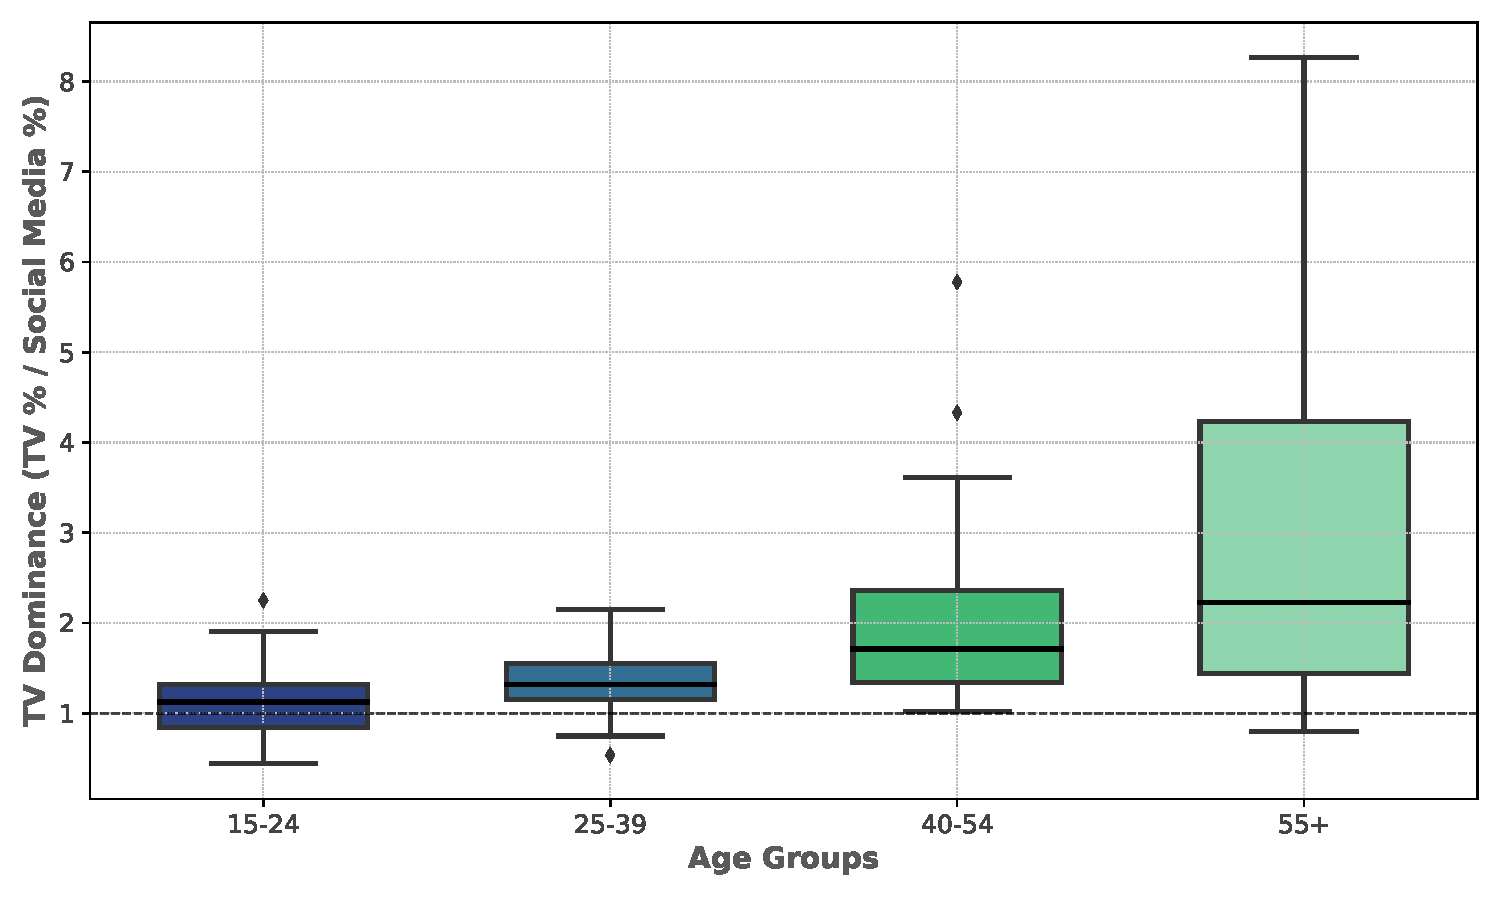
\includegraphics[width=130mm]{figures/age_cohorts_full}
		\caption*{\small \textit{Note:} Histogram of the preferred media used for political information in Europe. Using data for the 27 countries in Eurobarometer under the question \textit{"What media have you used the most to access news in the past 7 days?" }. $N=112059.$ 
			Source: Eurobarometer, 2022. }
		\label{fig:motivation2}
	\end{figure}
	
	
	

	
	
Traditional media still enjoy higher credibility than digital-only outlets or news encountered on social platforms. Europeans continue to cite television as their main source of current-affairs information, and nearly half (49 \%) say they trust public TV and radio—well above printed newspapers (39 \%) or news found on social networks and messaging apps (each below 15 \%) \citep{eurobarometer2022}. This credibility premium is closely linked to rising concern about fake news: respondents who worry most about disinformation are also the likeliest to turn to traditional broadcasters when verifying what is true. In the era of AI-enabled misinformation, audiences therefore continue to see traditional outlets—especially prime-time newscasts—as the safest gatekeepers of political information, underscoring the importance of analyzing these markets. 
	
%	https://www.europarl.europa.eu/news/es/press-room/20220704IPR34401/eurobarometro-los-europeos-confian-mas-en-los-medios-informativos-tradicionales
	
	
	
	
	
	\subsection{Spanish Politics and TV News}
	
	
	
Here, I provide context on the Spanish political party system to then contextualize the television news and the ideology of their audiences.

	
	
	
	\subsubsection*{Spanish Political Context}
	

	

	
	
	Political power in Spain has historically been dominated by a two-party system, with government alternating between the Socialist Party (PSOE) and the People’s Party (PP). During my sample period (December 2022–July 2023), Spain was governed by a PSOE-led coalition under President Pedro Sánchez, first in alliance with Unidas Podemos (UP) and, after its re-launch, SUMAR.\footnote{Relevant for this period of study is the integration of Podemos into the new party SUMAR. All classification metrics account for this transition, but throughout the text I refer to UP as either Podemos or SUMAR after its creation.} with the main opposition led by PP and the extreme right party VOX. Although regional and independentist parties play a major role in the political environment, they are excluded from this analysis. For the remainder of the paper, parties are pooled into two blocs: right (PP and VOX) and left (PSOE and UP).
	
	
	 The extreme-right party VOX made notable gains in the May 28, 2023 regional elections, fueling speculation of a PP–VOX coalition. In response to these results, the day after the regional elections, President Sánchez decided to bring forward the general elections to July 23, 2023. In that election, the PP emerged as the largest party in the Cortes, though without options to form an absolute majority, which led  the left coalition to maintain power. 
	
	
	
	
	
	
	
	
	
	
	\subsubsection*{Spanish TV News}
	
	
	The product analyzed in this paper is television news. I focus on the four largest national news channels: Televisión Española (TVE), the state‐owned public broadcaster; Antena 3 and La Sexta (Atresmedia group); and Telecinco (Mediaset). Altogether, their evening news editions capture around 50 \% of the market share—about 4.5 million viewers, or 10 \% of Spain’s population. By comparison, the most‐watched U.S. cable‐news program (Fox News) averages roughly 2.2 million  viewers. While these outlets drive the national news agenda, data limitations prevent inclusion of regional networks—most notably Catalonia’s TV3, which commands a substantial local audience and may exhibit distinct partisan dynamics. Future work can extend this framework to incorporate TV3 and other region‐specific channels.  
	


How does the audience of these programs look like politically?	Figure \ref{fig:opinion} shows the correlation between individuals' preferred political party (left or right) and their preferred channel for acquiring political information, based on survey data from the Centro de Investigaciones Sociológicas (CIS). I condition only on \textit{partisan} individuals, i.e. those that report a preferred political party. Right-wing individuals  tend to watch Antena 3 (A3) more, whereas left-leaning individuals are divided between La Sexta and the public channel TVE. Telecinco (T5)  appears in the middle, with weak correlations. This is consistent with the Mediaset group offering more pro-entertainment content as previously documented for Italy in \cite{durante_aer}.

	
	\begin{figure}[!htbp]
		\centering
		\caption{Correlation Between Preferred Channel and Political Party}
		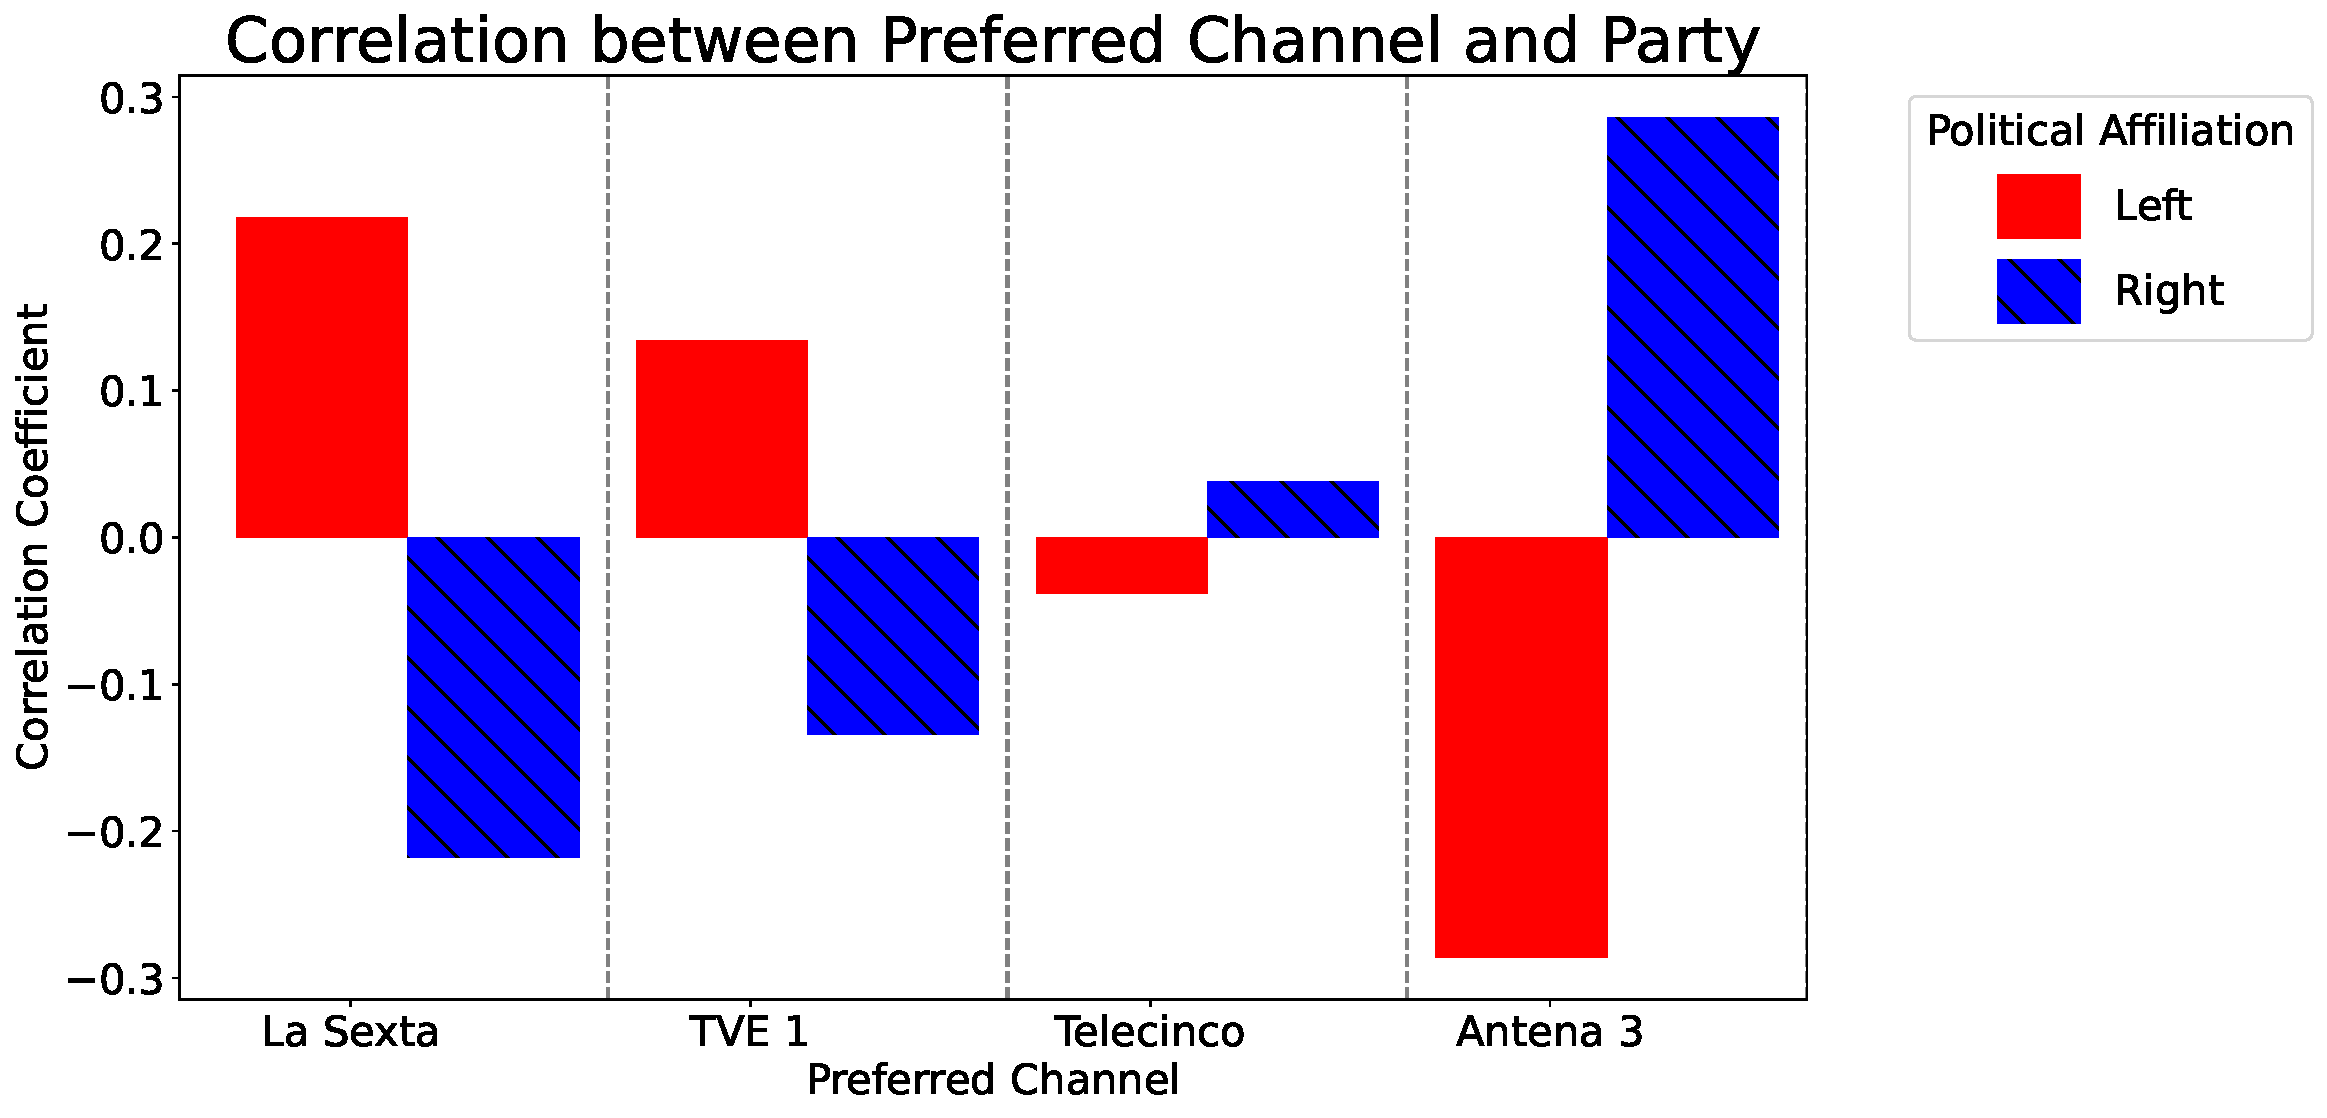
\includegraphics[width=120mm]{figures/corr_party_channel3}
		\caption*{\small \textit{Note:} Bars represent the correlation coefficient between the declared preferred political party (pooling left and right parties) and the most-watched channel. The survey asks respondents if they watch TV for political content  and what their preferred channel is. Source: Built using data from CIS's Encuesta Pre-electoral 2023.}
		\label{fig:opinion}
	\end{figure}
	
	

	
	
	
	To benchmark the degree of partisan sorting in television news against other media and prior studies, I compute the \emph{isolation index} \citep{gentzkow_isolation} for TV, radio, and the press. In a binary left–right setting, the index measures how much more likely a right-wing user is to encounter a co-partisan in the outlets right-wing audiences consume than a left-wing user would in the outlets left-wing audiences visit. An isolation index of zero indicates no additional clustering by ideology (i.e., right- and left-leaning viewers consume the same outlets), while an index of one corresponds to complete segregation, where each group encounters only its own members.% 
	The formal definition appears in Appendix Section~\ref{sec:isolation}. 
	
	Table~\ref{tab:isolation_table} reports the isolation index and its decomposition by party bloc. On television, right-wing exposure for right-wing viewers (i.e., the average right share of the outlets they watch) is 41\% compared to 30\% for left-wing viewers. 
	In the press, the figures are 43\% vs.\ 25\%, and on radio 52\% vs.\ 24\%.
	Accordingly, the index ranks television as the least isolated medium (11 pp), followed by the press (18 pp), with radio the most isolated (29 pp).
	
	To contextualize these results, Table~\ref{tab:isolation_table_compare} compares them with recent estimates for France in 2022 \citep{Dejean2022PartisanSE} and the U.S.\ in 2008 \citep{gentzkow_isolation}. Spain exhibits higher levels of partisan isolation across all media, consistent with the greater political polarization documented elsewhere \citep{edelman_trust_2023}.
	Television in Spain is about 8 percentage points more isolated (11.5 pp) than French TV (3.5 pp) or U.S.\ cable news (3.3 pp), and nearly 10 pp above U.S.\ broadcast TV (1.8 pp).
	
	Taken together, the cross-country ranking reproduces a common pattern: newspapers and radio are more ideologically segmented than broadcast TV, while Spain shows overall higher segregation. Since media effects are limited when audiences are already sorted, this pattern suggests greater potential for television to influence attitudes (given its comparatively mixed audience) and less for radio or newspapers, where audiences are already politically aligned. This distinction is crucial when considering the external validity of the polarization results presented here for other media environments.
	
	
	
	
	
	
	
	
	\section{Data and Descriptive Evidence}
	\label{sec:data}

	I assemble a unique dataset that captures both the demand and supply sides of TV news in Spain. For the demand side, I have minute-by-minute viewership data for the four main channels that offer daily news programs: TVE, A3, La Sexta, and T5. On the content side, I build a scraping pipeline that records the daily news programs live and processes this information into text. This dataset spans from December 2022 to July 2023 on a daily basis. It is complemented by all the stories published in Spanish by the largest news provider. Finally, I make use of survey and weather data as controls.
	
		\subsection{Data}
		
			\textbf{TV Content}
		
		I record daily  videos for both the midday and evening news editions. This leads to a total of 563 hours of content. I rely on Google Cloud infrastructure to store and process the data. Videos are converted to audio, and I use machine learning (\textit{speech-to-text}) to obtain text transcripts. Although visuals are not used in the main estimation due to computational constraints, I show comparisons between image and text metrics below. A summary of the entire downloading pipeline is provided in Appendix Section \ref{sec:appendix_models}.
		
		News programs offer a unique environment to test substitutability for several reasons. Even though channels offer other political programs, the homogeneity of these products allows for very clean comparisons. These programs are broadcast every day at almost the same time and all share a very similar structure, with a presenter introducing the main stories of the day. Their lengths are similar, with the shortest show (Antena 3) averaging 32 minutes and the longest (TVE) 42 minutes.
		
		TV news programs are also highly fact-checked and they remain the most trusted source of information in Spain.\footnote{The Digital News Report 2023 reveals notable patterns in public trust towards news media across Europe, with Spain reflecting a stable but modest level of confidence. According to the report, the public service broadcaster RTVE and Antena 3 Noticias continue to rank as the most trusted news sources, with trust levels of 48\% and 51\%, respectively. La Sexta registers  approximately 42\%, and Telecinco follows at 41\% \citep{reuters_dnr_2023}.} This fact is important as it ensures a cleaner interpretation of the audience choice data as revealed preferences for the content consumed and limits the extent of fake news as an additional dimension in the editorial strategy of the outlets. 
		
	
	\textbf{Audience Data}
	
	I use Audimeter, a high-frequency audience data source provided by Kantar Media. I observe the share of viewers for each channel at each day and minute. Variation over minutes will not be exploited. Instead, I rely on the initial audience at the beginning of the shows each day (i.e., minute-zero audience).
	Although I do not have individual-level data on choices, I have geographical disaggregation for 15 autonomous regions in Spain (also referred to as regions hereinafter), which I match to survey demographics.\footnote{The Canary Islands and La Rioja are excluded due to different time zones and zero market shares, respectively. Similarly, peak days with sport events that altered the news schedule were also removed.} The shares are specific to the evening TV news shows, which, with the exception of La Sexta at 20:00, start at 21:00 daily. For this analysis, this channel’s program is treated as if it occurred simultaneously with the others.
	
	%\footnote{This might pose problems in the substitutions toward the outside option and specifically with  \textit{connected substitutes} assumption in \cite{berry2013connected}. Specifically, invertibility of demand requires weak substitutatbility across  }
	

	
	\textbf{Agencia EFE}
	
	I obtain all news stories published in Spanish by one of the largest news agencies in the world, Agencia EFE. I have information on the title of each story along with a short summary segment for  32,525 stories in my sample period.
	
	Similar to Reuters or Associated Press, this agency mainly sells content and images to third-party newscasts. All the outlets in my sample are clients of Agencia EFE.\footnote{See collaborations with \href{https://www.telecinco.es/autores/agencia-efe/}{Mediaset}, \href{https://cadenaser.com/nacional/2024/09/22/el-teletexto-una-herramienta-olvidada-que-aun-perdura-en-nuestras-televisiones-cadena-ser/}{Atresmedia}, and \href{https://www.rtve.es/rtve/20130301/rtve-agencia-efe-firman-convenio-colaboracion/611440.shtml}{RTVE}.} 


	\textbf{Congress Speeches}

 I collect the complete set of plenary session transcripts from the Spanish Congress of Deputies during the XV Legislature. The official Diarios de Sesiones del Pleno are published in PDF format on the Congress website.\footnote{Available at: \url{https://www.congreso.es/es/busqueda-de-intervenciones}} . There are a total of $1411$ interventions. Each of them is linked to the corresponding speaker, and I match speakers to their parliamentary group using official records. This dataset is used for robustness of the text classification. 

	
	\textbf{Survey Data}
	
	To understand polarization behavior, I use survey data gathered from the Centro de Investigaciones Sociológicas (CIS). Specifically, I rely on the "intention to vote" question and map it onto my binary left–right spectrum according to the parties described above. These data are monthly and are in cross-sectional format.
	
	\textbf{Weather}
	
	I use meteorological data on daily rainfall deviations per region for the time span matching the TV news programs (18:00–00:00) from the Spanish Meteorological Agency (AEMET).
	

	
	
	
	\subsection{Text Classification}
	
	As noted above,  news programs present a very similar structure in length, broadcast time, and format. This homogeneity allows for cleaner comparisons as opposed to general opinion shows, where characteristics differ starkly, but at the same time make them almost perfect substitutes; the key differentiation (aside from vertical, quality components) being the way they treat the information. Here I describe how text analysis techniques can provide robust measures of political slant and effectively differentiate the outlets' treatment of  information. 
	

	
	\subsubsection*{Building Content Characteristics}
	
	Each day \(d\), channel \(j\) produces a set of stories \(S_{jd}\) indexed by \(s\). Empirically, these segments result from BERTopic clustering on the unstructured transcripts, which ensures that the LLM has enough context by feeding it the entire text of a given story. This leads to a total of 20,674 stories. The subset of political stories, \({P}_{jd}\subseteq S_{jd}\), is the set of all stories that mention national parties or prominent politicians in addition to general words related to politics, identified by keyword matches from Table~\ref{table:politics}.
	
	Each \(s\in {P}_{jd}\) is fed into ChatGPT and  assigned a score: \({t}(s)\in\{-1,0,1\}\)\footnote{More details about the prompt and classification results can be found in Appendix Section \ref{sec:appendix_models}.} with ${t}(s)=1$ (${t}(s)=-1$) denoting a positive (negative) tone. Stories with a stance (i.e., \({t}(s)\in\{-1,1\}\)) also receive a party label \({p}(s)\in\{L,R\}\), whereas neutral stories do not. 
	
	Notice that the broad classification of what is \emph{political} allows for stories that do not contain any specific mention of Spanish politics to have an associated slant toward some party.	Table~\ref{tab:international} contains examples of stories that lack any explicit reference to Spanish political actors yet still receive a partisan label. Positive Left stories include an economic forecast from the European Commission and the opening of a new gigafactory, while Negative Left stories include court officers barricading courthouses for pay raises and fuel-price surges driven by the Ukraine war. These cases show how the classifier infers slant from thematic framing alone, assigning a political slant to national parties without explicit references to them. 
	
	
	Additionally, a story can be mapped to its duration in minutes, \( {min}(s)\). This is key to accounting for the intensive margin. Combining all these characteristics—i.e., party label, tone, and minutes—I define the shares of positive and negative minutes, as well as the share of airtime devoted to politics, as follows:
	
	
	


		\begin{equation}\label{eq:controls}
		\begin{aligned}
			x_{jd}^{party+}&= \frac{1}{min_{jd}} \sum_{s \in S_{jd}}\bigg(\mathds{1}\{t(s)=1\} \times \mathds{1}\{p(s)=party\}\times min(s) \bigg) \quad \forall party \in \{L,R\} \\
			x_{jd}^{party-}&= \frac{1}{min_{jd}} \sum_{s \in S_{jd}}\bigg( \mathds{1}\{t(s)=-1\} \times \mathds{1}\{p(s)=party\} \times min(s)\bigg) \quad \forall party \in \{L,R\} \\
			x_{jd}^{political}&=\frac{1}{min_{jd}} \sum_{s \in P_{jd}}min(s).
		\end{aligned}
	\end{equation} 
	

	Similarly, I proxy the daily news landscape with all stories published in Spanish by \emph{Agencia EFE}—$N\approx32{,}000$ items over the sample. Mirroring the content covariates in~\eqref{eq:controls}, I classify every  story with the same NLP pipeline and construct daily measures of the political mix in the \emph{news landscape}:
	
	\begin{equation}\label{eq:efe}
		\begin{aligned}
			z_d^{\,party+} &= \frac{1}{|\mathcal{N}_d|}\sum_{s\in \mathcal{N}_d}
			\bigl[\mathds{1}\{t(s)=1\}\,\mathds{1}\{p(s)=\textit{party}\}\bigr]
			&\forall\,\textit{party}\in\{L,R\},\\
			z_d^{\,party-} &= \frac{1}{|\mathcal{N}_d|}\sum_{s\in \mathcal{N}_d}
			\bigl[\mathds{1}\{t(s)=-1\}\,\mathds{1}\{p(s)=\textit{party}\}\bigr]
			&\forall\,\textit{party}\in\{L,R\},\\
			z_d^{\,\text{political}} &= \frac{|\mathcal{P}_d|}{|\mathcal{N}_d|}.
		\end{aligned}
	\end{equation}
	
	where now \(\mathcal{N}_d\) denotes the total number of Agencia EFE stories on day~\(d\), and \(\mathcal{P}_d\) the subset of them classified as political under the same criteria as before.
	
	
	
		These variables will constitute the main controls and instruments for the empirical application in the next section. 
	

		\subsubsection*{Outlets' Slant}
	
	
	
	Figure \ref{fig:chat} plots each channel’s net average tone toward left‐ and right‐wing parties, calculated as the difference between positive and negative coverage from Equation \ref{eq:controls} over all sample period. Positive (negative) values indicate a net (un)favorable tone towards a party by that outlet. La Sexta and TVE tilt strongly pro-left, Telecinco sits near the center with a mild leftward bias, and Antena 3 is the only channel  with a slight pro-right balance. Perhaps strikingly, every channel exhibits a net negative tone toward the right-wing bloc, reflecting the fact that the PSOE–UP left coalition held office throughout my sample period. In practice, this meant an abundance of positive policy stories on the left and comparatively few favorable stories on the opposition, which pushes the average right-wing tone to be negative. 
	

	
		\begin{figure}[!htbp]
		\caption{Average Tone Across Channels and Parties}
		\centering
		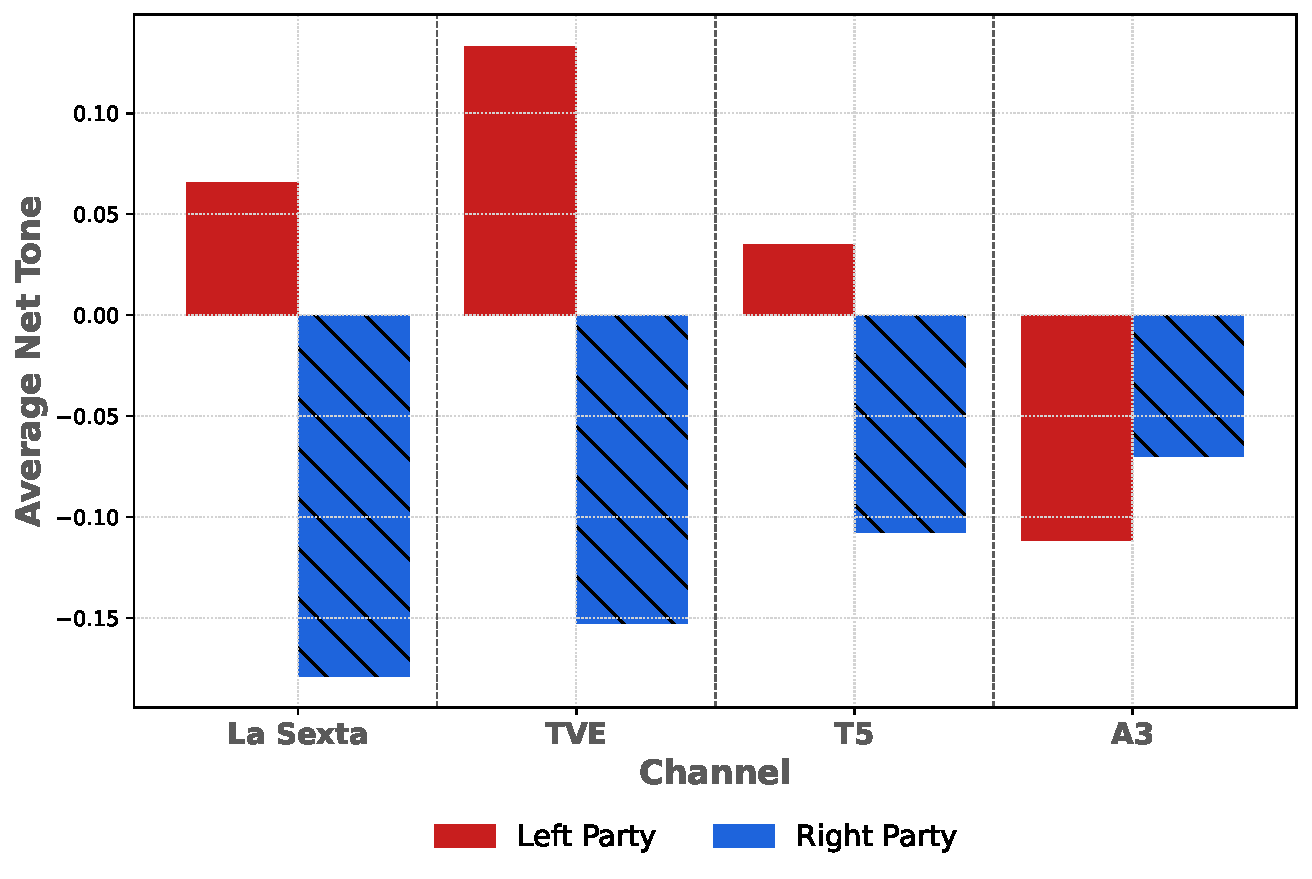
\includegraphics[width=120mm]{figures/chatgpt}
		\caption*{\small \textit{Note:} Average tone for each channel-party as classified by ChatGPT 4 from the whole sample period. The ideological score for channel $j$ on party  $p$ is computed as $	\bar{x}_j^{p+}-\bar{x}_j^{p-}$.}
		\label{fig:chat}
	\end{figure}
	
	
	
	
	To compare these supply‐side slant scores with audience ideology (demand), I assign each channel an \textit{ideology index} calculated as 
	
	
	
	\begin{equation}\label{eq:ideo_index}
		\begin{aligned}
			& Ideology_j \equiv \bigl(\bar{x}_j^{R+}-\bar{x}_j^{R-}\bigr)-\bigl(\bar{x}_j^{L+}-\bar{x}_j^{L-}\bigr),
		\end{aligned}
	\end{equation} 
	

and, in parallel, compute each region’s left–right position from the CIS survey correlations between party preference and channel choice shown above in Figure \ref{fig:opinion}. I then normalize both series so that the most extreme channels take values of $-1$ and $1$ to enable comparisons across the two different measures. Figure~\ref{fig:channel_ideology_lines} displays these normalized scores: panel~(a) shows outlets' positions based on viewers’ ideology, and panel~(b) based on their text‐based slant. The consistent left‐to‐right ranking and close scores in both panels confirms that the LLM‐based classification recovers the distribution of audience preferences, as one would expect in  a demand driven market equilibrium. Below, I also show robustness of the classification and comparisons with other methodologies previously used in the literature.
		
	
	
		\begin{figure}[!htbp]
		\centering
		\caption{Normalized Ideology Index by Channel}

		% Panel (a): ChatGPT-based
		\begin{minipage}[t]{0.49\textwidth}
			\centering
					(a) Demand: Viewers' ideology
		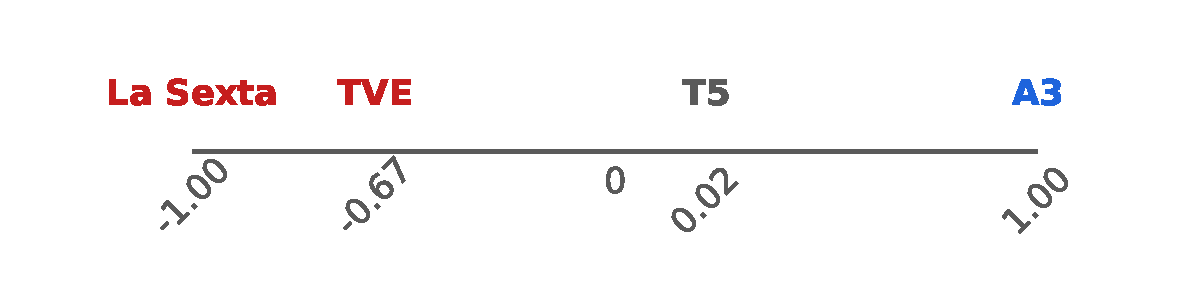
\includegraphics[width=\linewidth]{figures/congress_line_cis}
		\end{minipage}
		\hfill
		% Panel (b): CIS-based
		\begin{minipage}[t]{0.49\textwidth}
			\centering

			
				(b) Supply: Text classification
			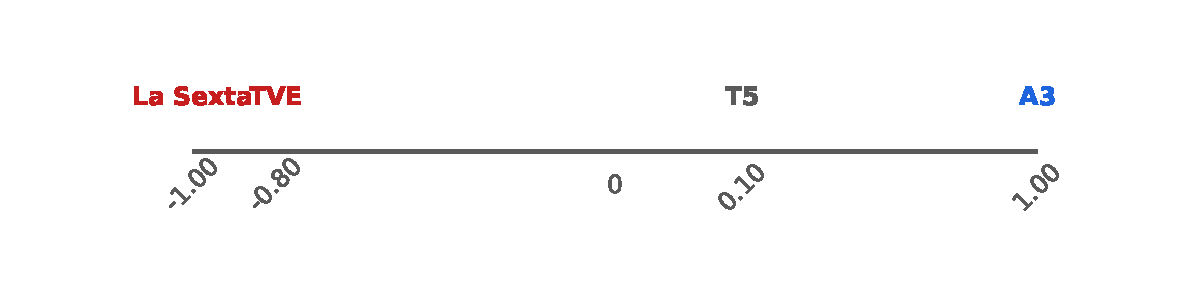
\includegraphics[width=\linewidth]{figures/congress_line_chatgpt}
			
			
		\end{minipage}
		
		
		\caption*{\small \textit{Note:} The figure compares normalized left–right positions for the outlets in the sample. Panel (a) uses viewer ideology data from CIS survey data, using the difference in correlation coefficients between right and left; panel (b) uses ChatGPT-based text classification net tone as described in Equation \ref{eq:ideo_index}. Values are normalized so that the two most extreme channels take values -1 and 1. }
		\label{fig:channel_ideology_lines}
	\end{figure}
	
	

	
	
		\subsubsection*{Political Coverage and the Election Campaign}
		
		
		
	
I divide the sample into two periods. The \textit{off-campaign} period runs from the start of data collection (December 2022) to May 13, 2023, the date of the first publicly announced campaign for the regional elections. The \textit{campaign} period covers both the regional and general election campaigns and ends on July 23, 2023 (general election day).

	
	Figure \ref{fig:coverage} plots the share of political content over time. The shaded area marks the campaign; vertical dashed lines indicate (i) campaign start, (ii) regional elections, and (iii) general elections. The dashed line is the average across the four TV channels (with a shaded band for one standard deviation) represented on the right y-axis, and the solid black line is Agencia EFE with the left y-axis representing the proportion of political stories on a given day. Both series display similar seasonality (Pearson correlation $r=0.59$), dipping when non-political events dominate (Christmas, Easter). On average, TV channels devote 18\% of airtime to politics in off-campaign, rising to 30\% during the campaign. For EFE, the share of political stories increases from 43\% to 51\%.
	
	Table \ref{tab:correlations} shows that this aggregate correlation masks heterogeneity across outlets. Antena~3 exhibits the strongest co-movement with EFE in political coverage ($r=0.67$), followed by Telecinco ($r=0.48$), TVE ($r=0.38$), and La Sexta ($r=0.26$).
	
	%	Figure \ref{fig:coverage} plots  the share of political content over time. The shaded area marks the campaign; vertical dashed lines indicate (i) campaign start, (ii) regional elections, and (iii) general elections. The dashed  line is the average across the four TV channels (with a shaded band for one standard deviation) represented in the right y-axis, and the solid black line is Agencia EFE with the left y-axis representing the proportion of political stories on a given day. 
		%Both series display similar seasonality (i.e Pearson correlation of $0.589$), dipping when non-political events dominate (Christmas, Easter). On average, TV channels devote 18\% of airtime to politics in off-campaign, rising to 30\% during the campaign. For EFE, the share of political stories increases from 43\% to 51\%.
	




	
	\begin{comment}
		\begin{tabular}{lcc}
			\toprule
			\textbf{Outlet} & \textbf{Pre-campaign} & \textbf{During campaign} \\
			\midrule
			A3 & 0.263 & 0.399 \\
			TVE & 0.126 & 0.179 \\
			LA6 & 0.173 & 0.252 \\
			T5 & 0.136 & 0.237 \\
			\addlinespace
			EFE (Factiva) & 0.432 & 0.508 \\
			\bottomrule
		\end{tabular}
	\end{comment}
 
	
	
	\begin{figure}[!htb]
		\caption{Proportion of Political Coverage over Time}
		\centering
		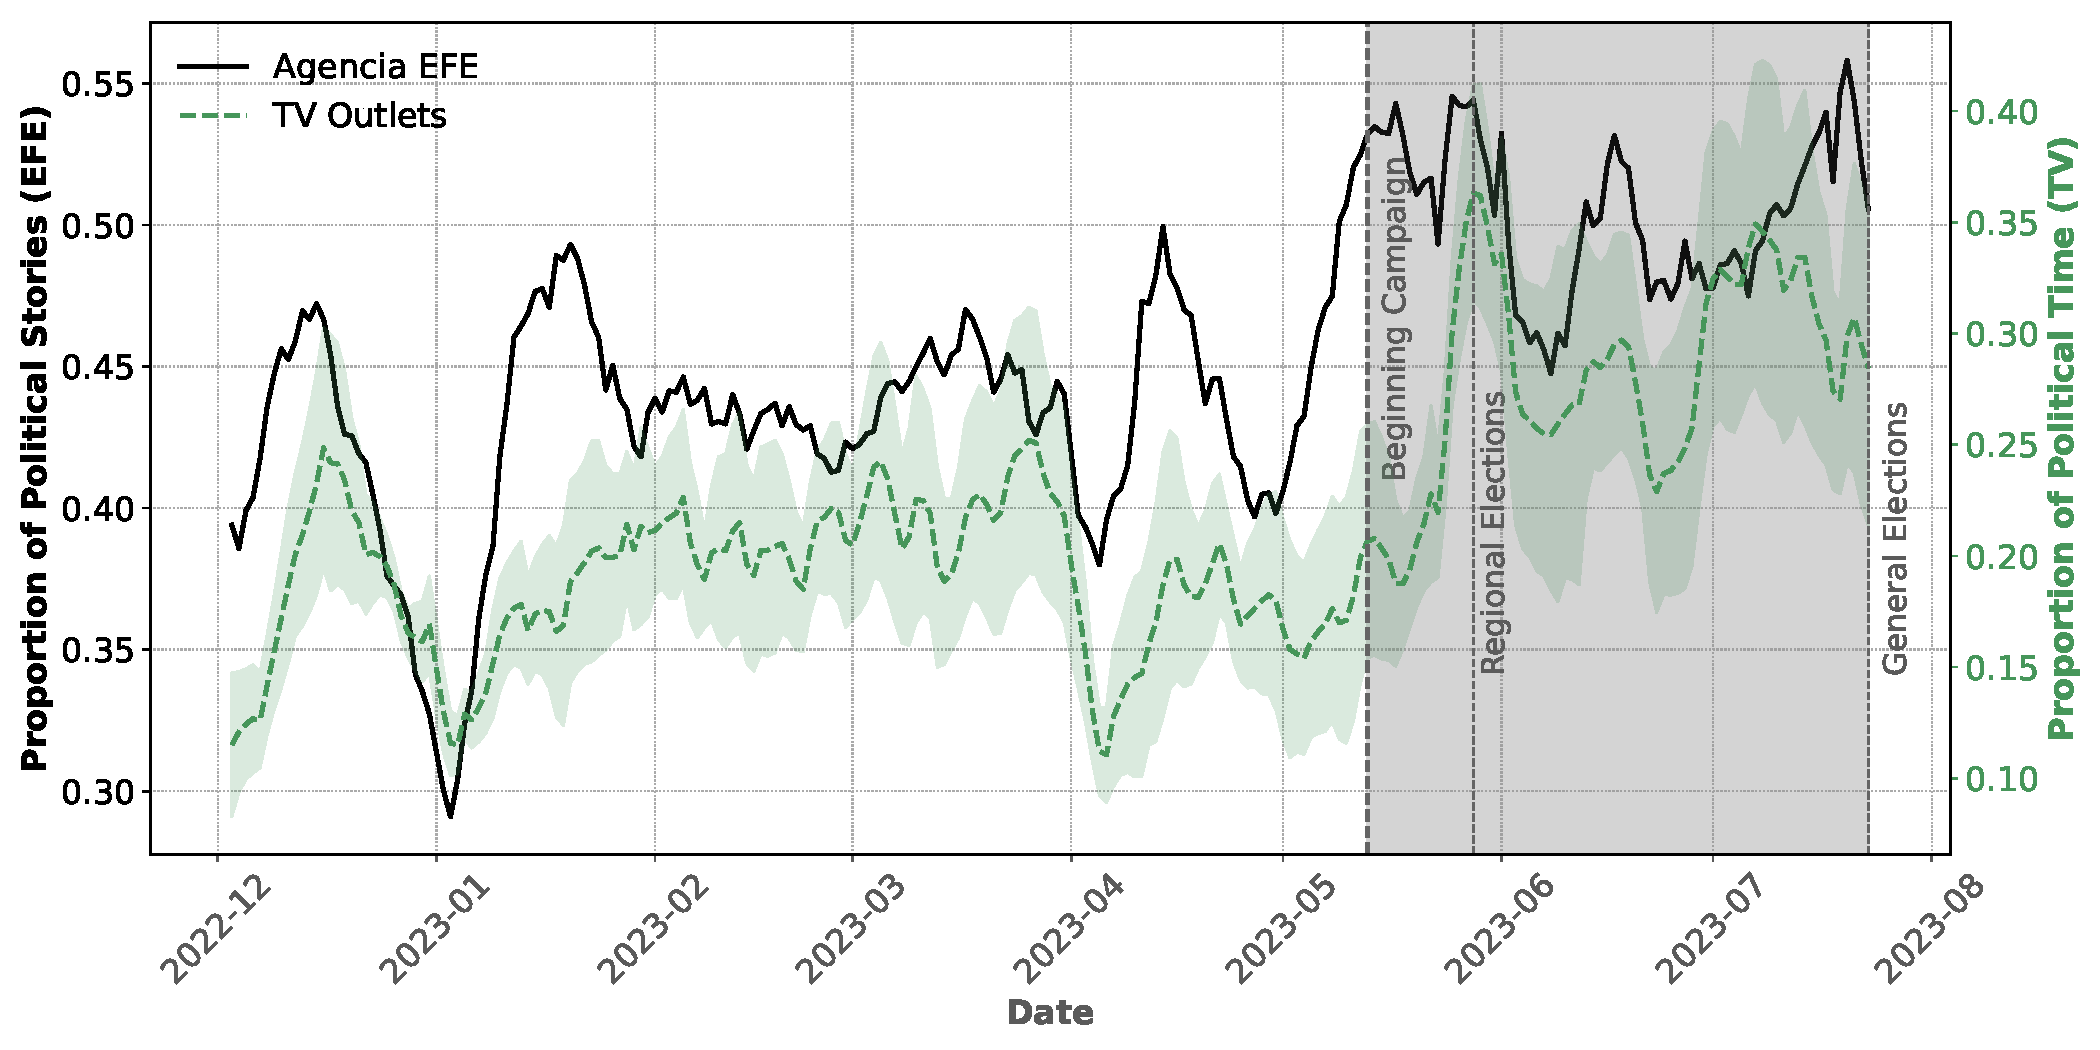
\includegraphics[width=150mm]{figures/political_words_bothv2}
		\caption*{\small \textit{Note:} The figure represents the proportion of political content for the TV outlets (dashed) and Agencia EFE (solid). Political time is measured by dictionary matches to terms in Table \ref{table:politics}. For the TV outlets, the proportion of political time is the fraction of political minutes over total minutes. Shaded area represents the standard deviations. For Agencia EFE (solid line), the proportion of political content is the share of political stories. Vertical, dashed lines indicate the date of the beginning of the campaign, the regional and the general elections, respectively. The shaded area represents the \textit{campaign} period considered. Both time series present a Pearson correlation of $0.589$.}
		\label{fig:coverage}
	\end{figure}
	
\begin{comment}
	content...

\begin{table}[!htbp]
	\centering
	\caption{Proportion of Political Content}
	\begin{tabular}{lcc}
		\toprule
		\textbf{Outlet} & \textbf{Pre-campaign} & \textbf{During campaign} \\
		\midrule
		La Sexta & 0.173 & 0.252 \\
				TVE & 0.126 & 0.179 \\
		T5 & 0.136 & 0.237 \\
				A3 & 0.263 & 0.399 \\
		\addlinespace
		\hline
		Agencia EFE & 0.247 & 0.316 \\
		\bottomrule
	\end{tabular}
\caption*{\small \textit{Note:} The table shows the proportion of political content for the four TV channels, calculated as the proportion of time spent in politics; and for the Agencia EFE, calculated as the proportion of stories that are political. }
\label{tab:tests}
\end{table}
\end{comment}
	
	
	
		%	\subsubsection*{Political Slant and the Election Campaign}


%Outlets track closely the newswire in terms of political coverage. Does the slant of the outlets also match that of the Agency? How do left and right outlets react to key political events? Figure \ref{fig:net_tone} shows the ideological index from equation \ref{eq:ideo_index} for Agencia EFE (solid, black line) compared to the left and right outlets \footnote{Figure \ref{fig:net_tone_by_channel} on the Appendix shows the decomposition by outlet and Table~\ref{tab:political_sentiment_types} shows the decomposition of the proportion of minutes spent by content category for each outlet and for Agencia EFE, in both the campaign and off-campaign periods. }. Positive (negative) values indicate coverage favorable to the right (left). Three facts emerge. {First}, EFE’s series is predominantly negative (more favorable to the left on average). {Second}, similar to the political coverage, outlets co-move with the wire. Table \ref{tab:correlations} shows the pearson correlation coefficient of the time series by outlet. Antena 3 and TVE present the highest pearson correlation values  XXX (insert pearson values) follows by La Sexta and Telecinco. 



%{Third}, co-movement around salient events appears 
% asymmetric under some key events. For isntance,  the late-May rightward swing (regional elections) is amplified by Antena~3, and the early-March leftward dip (International Women’s Day and the failed no-confidence motion) is amplified by La~Sexta/TVE. However, there are counterexamples—notably a brief May uptick in the left series driven by TVE—so the asymmetry is not systematic. This motivates a formal test of asymmetric responsiveness below, and the resulting time variation is central to the identification strategy in Section~\ref{sec:identification}.



Turning to the ideological index from Equation \ref{eq:ideo_index}, Figure \ref{fig:net_tone} shows the smoothed time series for Agencia EFE (solid black line) and for the main outlets.\footnote{Figure \ref{fig:net_tone_by_channel} in the Appendix shows the decomposition by outlet, and Table \ref{tab:political_sentiment_types} reports the proportion of minutes spent by content category for each outlet and for Agencia EFE, both during and outside the campaign period.} Positive (negative) values indicate coverage more favorable to the right (left). Two facts stand out. {First}, EFE’s series is predominantly negative, indicating a systematic tilt toward the left on average. {Second}, outlets also co-move with the wire, though correlations are weaker than for political coverage. The right-leaning Antena~3 shows the strongest co-movement with EFE ($r=0.36$); the left-leaning channels TVE and La Sexta follow ($r=0.32$ and $r=0.24$, respectively), while Telecinco, consistent with its middle position, exhibits a very small correlation ($r=0.02$).


\begin{figure}[!htb]
	\caption{Evolution of the Ideological Index}
	\centering
	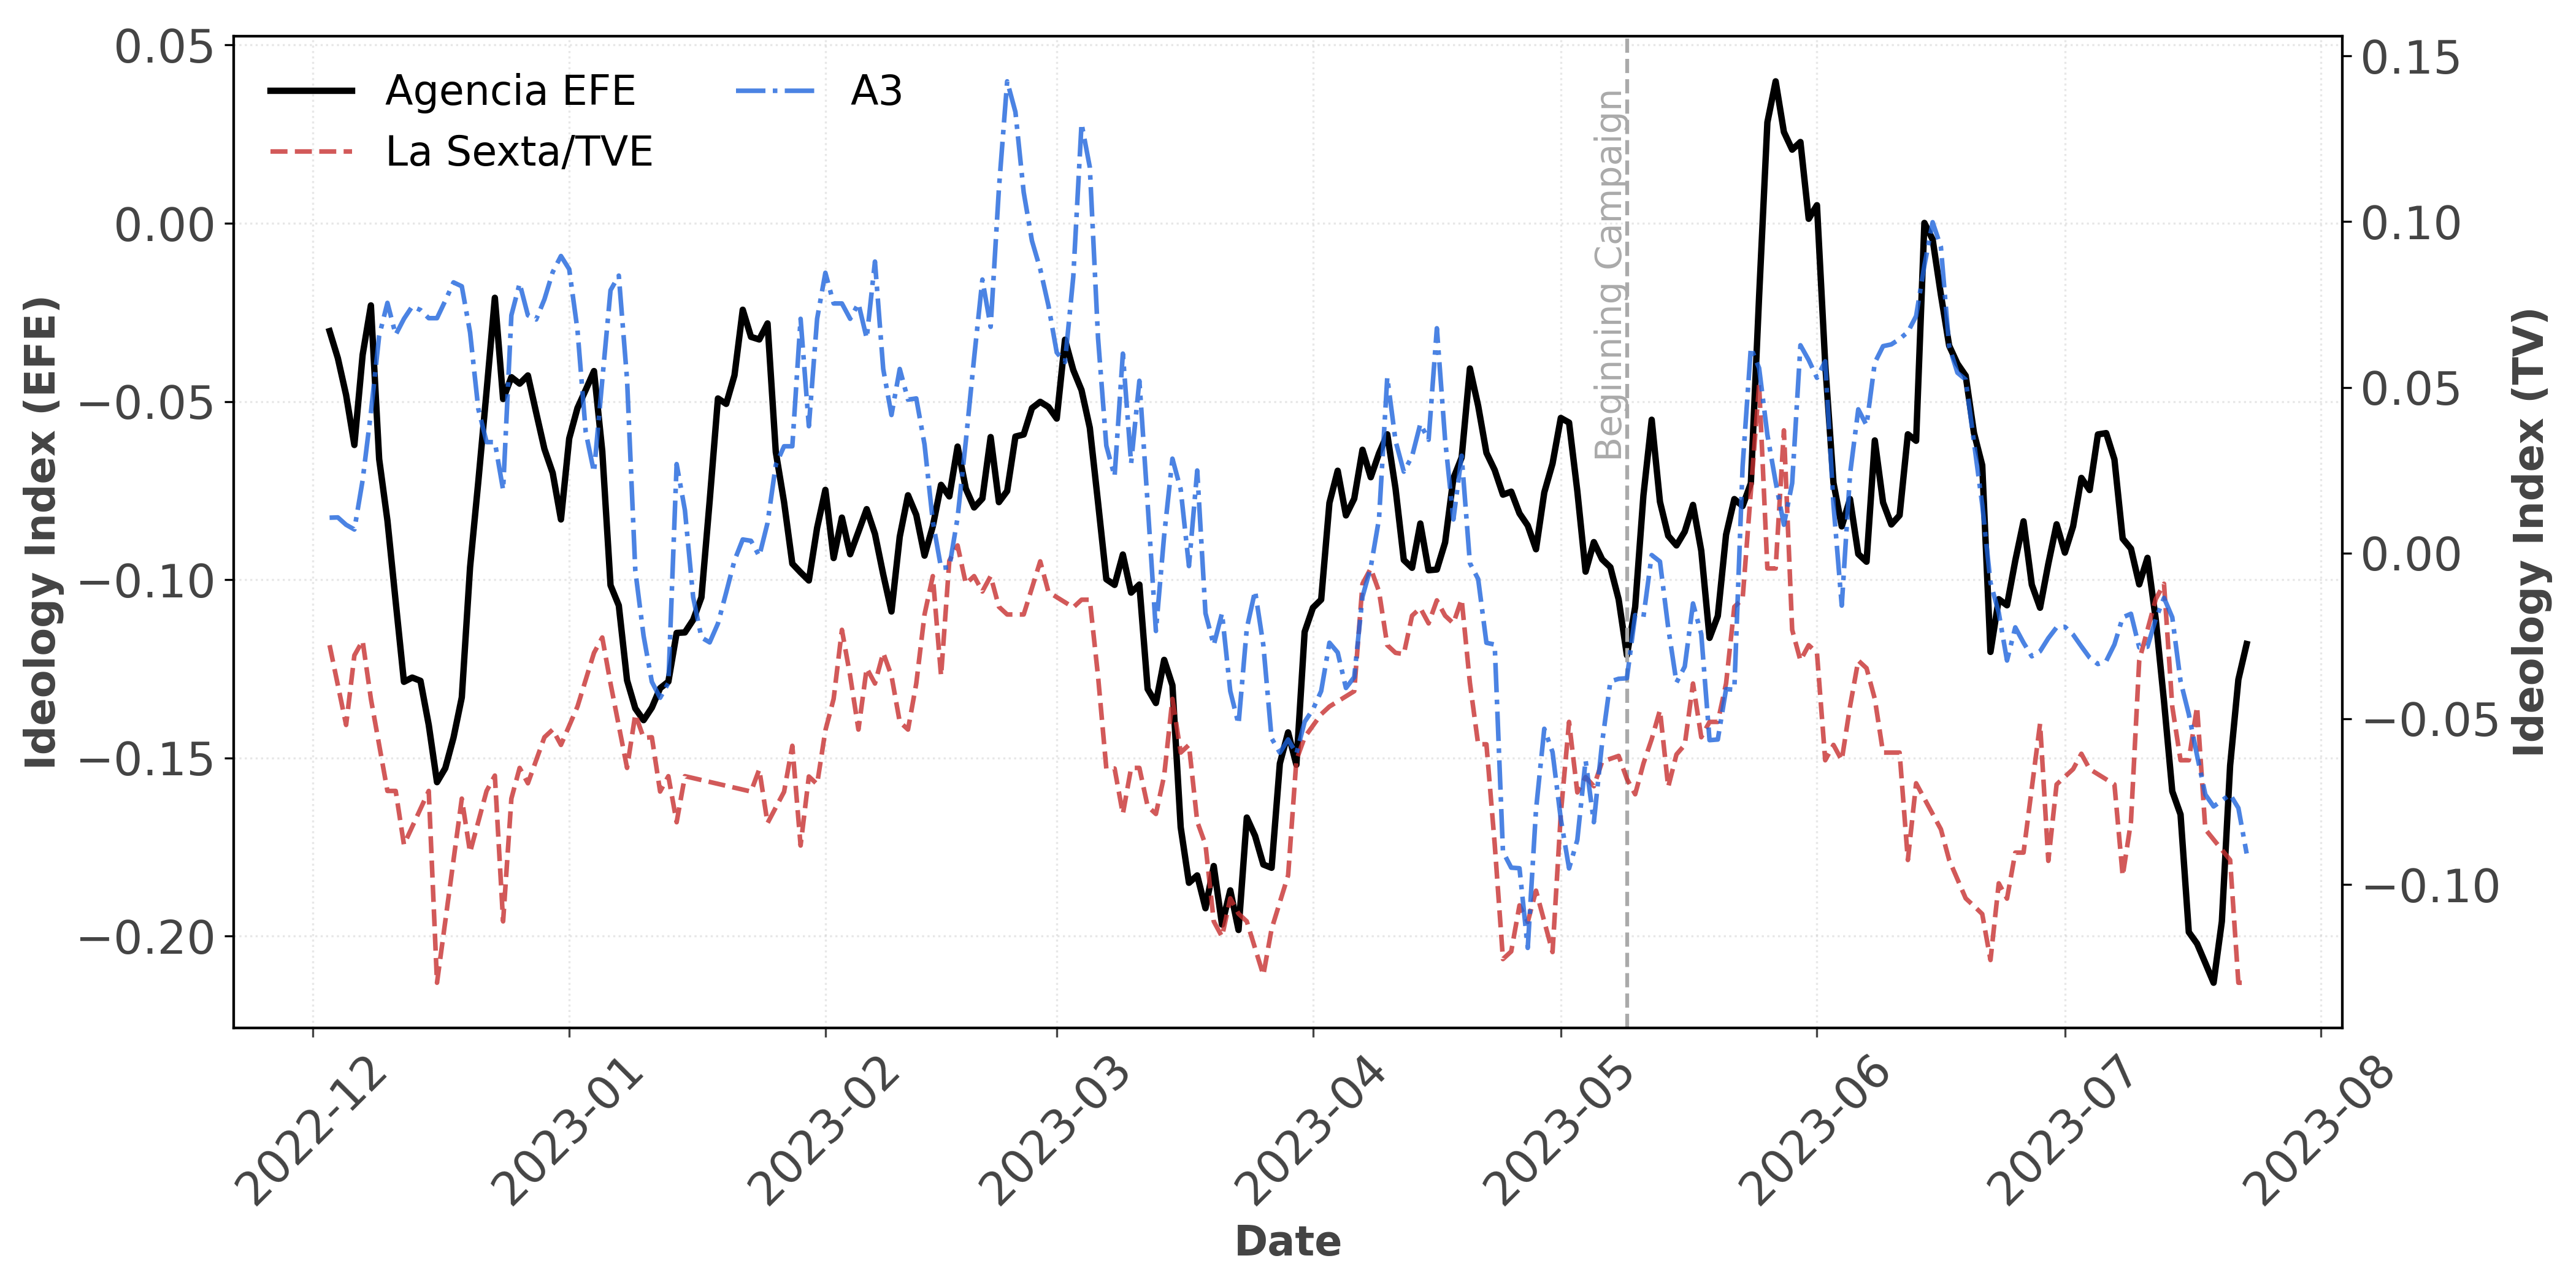
\includegraphics[width=150mm]{figures/tv_vs_efe_net_diff}
	\caption*{\small \textit{Note:}The figure represents the smoothed time series of the ideology index in Equation \ref{eq:ideo_index} for TV channels (right y-axis) and the analogous formula for Agencia EFE (solid) on the left axis. For visual purposes, left channels (La Sexta and TVE) are pooled and represented by the dashed red line. The right-wing channel is represented by the dotted blue line. All series are smoothed using a centered rolling mean with a 9-day window to reduce noise and highlight underlying trends over time.}
	\label{fig:net_tone}
\end{figure}

Finally, the figure suggests that some swings around salient political events. For instance,  the late-May rightward swing (regional elections) is amplified by Antena~3, and the early-March leftward dip (International Women’s Day and the failed no-confidence motion of the Right) is amplified by La~Sexta/TVE.  This motivates a closer, formal analysis of asymmetric responsiveness, which I develop in Section~\ref{sec:identification}.



The rise of negative campaigning has been extensively documented \citep{lau2009negative}. Candidates increasingly attack their opponents, and these messages are recycled by the media \citep{iyengar_affective}, often reinforcing partisan divides in coverage.

Table \ref{tab:political_sentiment_types} reports the composition of political tone accompanying this convergence. Focusing first on Agencia EFE, the newswire increased the share of stories across nearly all tone categories, with the sole exception of negative coverage of the left. The dominant tone remained favorable stories about the left, followed by favorable coverage of the right. Turning to the television outlets, a consistent pattern emerges: all of them (i) reduced their use of negative tone toward the left, while (ii) expanding the share of negative minutes about the right. Furthermore, Figure \ref{fig:tone_by_party} shows that this common strategy is driven by the extreme parties on the left and right of the spectrum: All outlets become more negative on the extreme right party VOX and more positive on the left party SUMAR.

  Did these shifts translate into a more polarized political spectrum? To address this, I replicate Figure \ref{fig:channel_ideology_lines} and track changes in slant from the off-campaign period to the campaign. Figure \ref{fig:change_line} illustrates the movement from dots (off-campaign) to crosses (campaign). The newswire EFE (not shown in the figure) moved toward the right, shifting from –0.17 to –0.13. This movement was mirrored only by the publicly owned channel TVE, which repositioned toward the center, whereas all other outlets shifted to the left.\footnote{Average relative tone by period is shown in Appendix Figure \ref{fig:tone2}.}


	\begin{figure}[!htb]
		\centering
		\caption{Change in Positions Off-campaign to Campaign}
		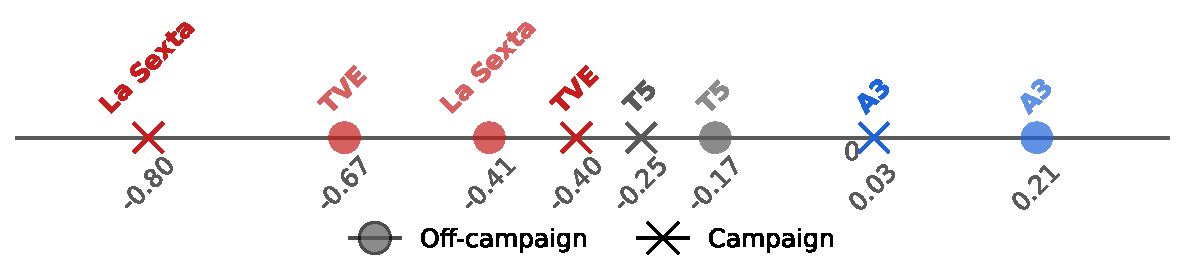
\includegraphics[width=100mm]{figures/congress_line_chatgpt_pre_postv2}
		
		\caption*{\small \textit{Note:} The figure shows the relative change in  slant positions  according to the ideological index in Equation \ref{eq:ideo_index} from off-campaign to campaign. }% Values are normalized so that the two most extreme positions take values -1 and 1 in the off-campaign period. }
		\label{fig:change_line}
	\end{figure}
	
	
Quantitatively, dispersion across channels narrowed slightly during the campaign\footnote{Dispersion is summarized using three complementary statistics. The cross-channel range measures the distance between the most right- and most left-leaning outlet. The standard deviation summarizes overall spread across outlets relative to the mean. Finally, the left–right bloc gap compares the average position of Antena 3 (the only right-leaning outlet) with the average of the three other channels (La Sexta, TVE, and Telecinco).}: the cross-channel range declined from 0.088 to 0.083, and the standard deviation from 0.032 to 0.030. Likewise, the left–right bloc gap (Antena 3 versus the other three channels) fell from 0.063 to 0.051. In short, rather than diverging further, outlets’ supply-side positions converged modestly during the campaign.
	

	
	
	
	
	
	
	
	
	
	
	\paragraph{Robustness of the text classification}
	
The use of LLMs as classifiers has gained popularity in recent years for various contexts, such as the classification of political stances, and they have even been found to achieve higher accuracy scores for ideological classification compared to human annotators \citep[see e.g.][]{lemens,tornberg2023,Gilardi2023ChatGPTOC}. However, two main concerns arise. First, LLMs have been shown to suffer from prompt instability, producing inconsistent results across multiple runs of the same prompt. Second, one may question the performance of alternative text classification methods. In Appendix Section~\ref{sec:robustness}, I address these concerns. I first demonstrate that the classification remains stable under repeated queries. Second, I compare my results with previous methods used to assess slant. Specifically, methods based on similarity to congressional speeches \citep{gentzkow2010media,laver2003extracting} yield a consistent ideological ranking of the outlets. I also apply face recognition to compare the slant measure with the standard metric based on politicians’ airtime. This metric, widely used by regulatory agencies and in prior research, produces a completely different scenario in which all channels appear more homogeneous and fails to predict actual slant.

Taken together, these results show the robustness of LLMs for slant classification and raise concerns about the use of traditional measures—such as image-based metrics—to assess plurality. Nevertheless, empirical validation with human annotators remains advisable for future work.

	
	

	
	
	\section{Demand for News}	\label{sec:demand}

In this section, I introduce the market setting for demand. Supply will be explicitly modeled in Section \ref{sec:supply}. I first develop a mixed logit (BLP) model \citep{berry_blp} where individuals choose the channel to watch depending on the content characteristic offered by the outlets (i.e political slant). I then present the endogeneity problem that arises from the simultaneity in editorial decisions and viewer's choices and introduce my identification strategy. Finally, I present the main estimation results and evidence linking media polarization to political polarization. 

	\subsection{Demand Model}

There are no ads during the newscasts, so I abstract from two-sided market considerations. Channels differentiate themselves by how they present the day’s stories, and viewers choose a single outlet to watch. The single-product choice assumption might be particularly strong in television markets, where viewers can explore different alternatives—something that cannot be identified from daily, aggregate data. To mitigate this concern, I restrict attention to the initial (i.e., minute-0) audience each day. Since three of the four outlets coincide in their airing times, the single-product choice assumption is less stringent: individuals must pick one channel to begin consuming the news\footnote{Previous works have documented the importance of inertia from previous shows in TV news consumption \citep{richter2025structural}. During my sample period, there were no changes in the preceding slot's programming agenda, which minimizes this concern. results are robust to the estimation using the first five minutes of the shows. }.



	An individual $ i $  in region $r$ chooses an outlet $ j \in \mathcal{J}\equiv \{La \ Sexta,TVE,Telecinco,A3\}$ \footnote{Although both La Sexta and A3 belong to the same media company, AtresMedia; the analysis here is based on short run profit maximization and they are assumed to be different, independent products. } to watch at the beginning of day $d$ based on the following expected utility : 
	
	
	\begin{equation}\label{eq:utility}
		\begin{aligned}
			& U_{ijrd}= \underbrace{\sum_k x_{jd-1}^k\beta^k+w_{rd}   \gamma  +  \xi_{jrd}}_{\delta_{jrd}}  + \underbrace{  \sum_k x_{jd-1}^k \Big( \sigma^k \nu_{ird}^k  + \pi^ky_{irm} \Big)}_{\mu_{ijrd}}+\epsilon_{ijrd} 
		\end{aligned}
	\end{equation} 
	
	where $ x_{jd}^k $ represents the  proportion of time on channel $ j $ and day $ d$ devoted to characteristic $ k \in \{R+,R-,L+,L-,political\}$ as defined in Equation \ref{eq:controls}. $w_{rd}$ measures the precipitation level on a given day-region. Weather conditions alter the value of the outside option and make viewers more prone to engage in indoor activities like TV consumption \citep{wilbur}. In my model, this happens with a common shift in the valuation of the inside options. 
	
	I model the distribution of viewers' content taste parameters using the standard normal random shocks $ \nu_{ird}^k \sim N(0,1)$ with mean shifted by  demographics, $ y_{irm} $, that represent whether individual $i$ in region $r$ is right-wing in month $m$ according to survey data.	The parameters $\pi^k$ allow for asymmetric tastes of politics based on ideology. Thus, they capture polarization in news consumption: More right wing individuals might screen out opposed content. 

The unobserved (to the econometrician) product characteristics are decomposed into $\xi_{jrd}= \xi_j + \xi_{dow} + \Delta \xi_{jrd}$, where I include product dummies that account for unobserved quality factors and day of the week dummies to control for  seasonal variation in the value of TV consumption. Unobserved product tastes can take the form of higher valuation of a given type of story that comes from knowledge of it through social media, specific regional taste shocks due to local events, non-controlled amplification due to visuals and appearance etc. By assumption, both the outlets and the viewers have full information about all the product characteristics. Due to timing differences, this assumption comes in the form of a correct expectation formation for next day unobserved preferences $ \xi_{jrd+1}$ in the moment of setting todays' content $\bm{x_{jd}}$. 
	
	The outside option is modeled in terms of \textit{potential} audience  \citep{berry1994estimating} and its mean utility value is normalized to 0 .
	
	Market shares are just the integral over the individual choice indicators from \ref{eq:utility}:  
	
	
	\begin{equation}\label{eq:shares}
	\begin{aligned}
		& s_{jrd} = \int d_{ijrd}(\bm{\delta_{rd}},\bm{\mu_{ird}})d\bm{\mu}_{ird}d\bm{\epsilon}_{ird}
	\end{aligned} 
\end{equation} 
	
	where $d_{ijrd}$ equals $1$ if $U_{ijrd}>U_{ikrd} \quad \forall j\neq k$ and $0$ otherwise. Survey weights are included in the integration.\footnote{The model is estimated using the \textit{pyblp} package \citep{conlon2020best}.} 

Under the assumption of no individual heterogeneity in preferences  ($\bm{\sigma}=0$) nor in  the distribution of ideology in a given region ($y_{ir}= \bar{y_r}$),  equation \ref{eq:utility} is consistent with a plain logit model as:


\begin{equation}\label{eq:logit}
	\begin{aligned}
		& ln \left(\frac{s_{jrd}}{s_{0rd}}\right)= \sum_k x_{jd-1}^k\beta^k+w_{rd}   \gamma  +\sum_k \left(x_{jd-1}^k\times y_r \right) \phi^k +  \xi_{jrd}
	\end{aligned} 
\end{equation} 


I show results under both the BLP and  logit models in  Section \ref{sec:results}. 
	
	\subsection{Endogeneity and Identification Strategy} \label{sec:endogeneity}
	\label{sec:identification}
	Models of demand estimation have often treated product characteristics as exogenous and used them as instruments for estimating price elasticities. While this might be true in markets where characteristics are costly to change and competition relies mainly on price after products are launched, content exogeneity is not credible in my setup: channels tilt the day's slant according to their audiences' preferences.
	
	Formally, viewers form expectations about each channel’s utility based on exogenous variables—weather, individual attributes, and an unobserved (to the econometrician) shock~$\xi$—as well as yesterday’s content slant~$\bm{x}_{jd}$. Channels, in turn, choose today’s slant while forecasting tomorrow’s utility shock~$\Delta\xi_{j,d+1}$. Hence, their optimal content decisions are functions of unobserved taste shocks, implying $\E[\mathbf{x}_{jrd}\,\Delta\xi_{jrd+1}] \neq \mathbf{0}$.
	
	To overcome this problem, I instrument every endogenous product characteristic~$k$ with exogenous supply shocks. Television stations rely heavily on third-party wire services for footage, text, and images, a downstream flow documented and exploited for U.S. newspapers in earlier work \citep{milena}. The fact that all outlets in my sample contract with EFE mitigates concerns that the agency is systematically biased or poorly informed. The goal, therefore, is not to proxy the outlet-specific news landscape perfectly but to exploit variation across days in each outlet’s ability to produce content.
	
	
	
	
The \emph{news shock} \(\bm{z}_d\) as defined in \ref{eq:efe},     is common to all outlets on a given day but affects them asymmetrically. Channels would like to produce at their steady-state, average positions (i.e., those depicted in Figure~\ref{fig:channel_ideology_lines}), but in the short run the available story mix constrains what they can cover. Since I assume daily content follows a random process and channels are aware of this, they smooth out variations in the news landscape by taking advantage of favorable days. This mechanism was partly shown in Figure \ref{fig:net_tone}, where the peak variations in Agencia EFE were taken advantage of by left- or right-leaning outlets accordingly.

	Tables \ref{tab:neg_left_channels} and \ref{tab:neg_right_channels} illustrate this mechanism by linking the news landscape to outlets’ reporting. Two days illustrate the asymmetry. On {27 February 2023} (the highest $z_d^{L-}$ in the sample), a loophole in a law sponsored by UP led to early releases of convicted sexual offenders and corruption scandals hurt the Socialist Party. Airtime devoted to negative left-wing stories differed markedly across channels: Antena~3 (right) devoted almost 19\%, TVE (left) and Telecinco each gave roughly 4\%, and La Sexta (left) about 2\%. The mirror image occurred on {17 May 2023} (the most negative day for right-wing parties): stories included a payments scandal involving the People’s Party, the defeat of a conservative motion in the Senate, and police-abuse allegations during an anti-VOX march. Left-leaning outlets devoted about 15\% of airtime to negative right-wing content, whereas Antena~3 devoted roughly 4\%.
	
	That there is exogenous variation across outlets is of practical importance for estimation and is required by the rank condition \citep{berry_haile_econometrica}. To show formal evidence, for each $(\text{party},\text{tone})$ pair I estimate separate regressions of the form:
	
	
	
	
	
	
	
	

	
	\begin{comment}
	\begin{figure}[h!]
		\caption{Trade-offs in the model}
		\label{fig:diagram}
		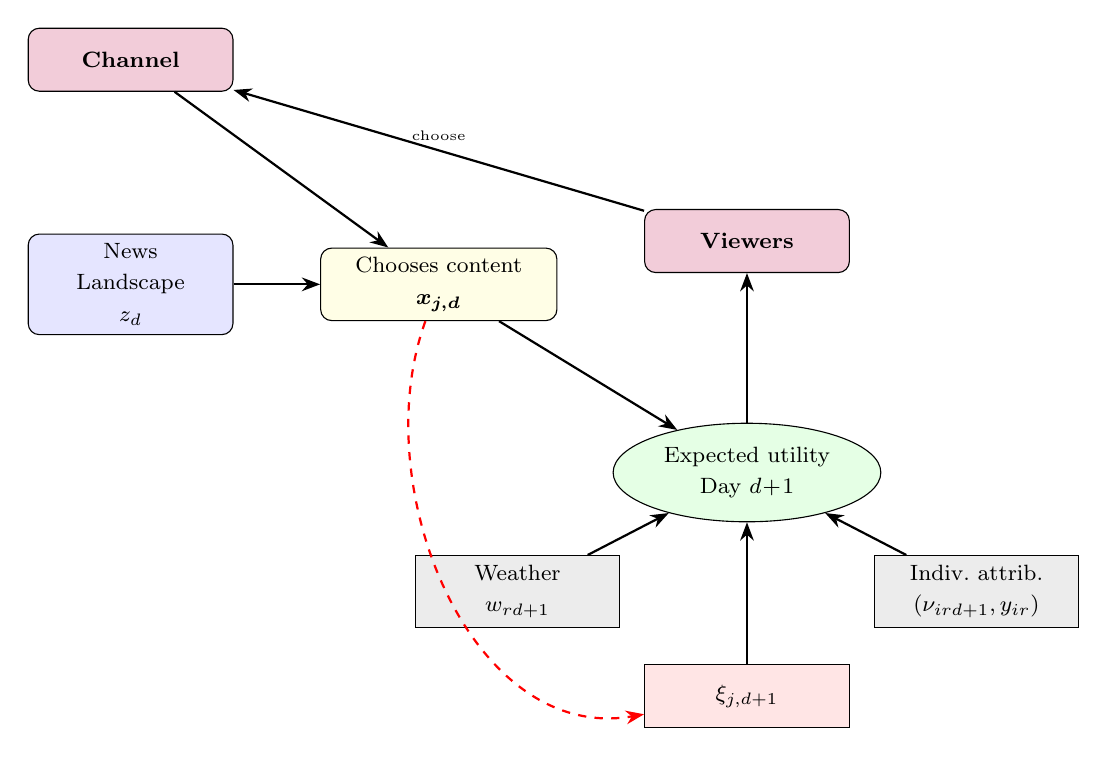
\begin{tikzpicture}[
			inst/.style   ={rectangle, draw, fill=blue!10,  rounded corners, align=center,
				minimum width=2.6cm, minimum height=0.8cm},
			decision/.style={rectangle, draw, fill=yellow!10, rounded corners, align=center,
				minimum width=3.0cm, minimum height=0.9cm},
			util/.style   ={ellipse,   draw, fill=green!10,  align=center,
				minimum width=3.4cm, minimum height=1.0cm},
			shock/.style  ={rectangle, draw, fill=red!10,   align=center,
				minimum width=2.6cm, minimum height=0.8cm},
			exo/.style    ={rectangle, draw, fill=gray!15,  align=center,
				minimum width=2.6cm, minimum height=0.8cm},
			actor/.style  ={rectangle, draw, fill=purple!20, rounded corners, align=center,
				minimum width=2.6cm, minimum height=0.8cm},
			flow/.style   ={-Stealth, thick},
			feed/.style   ={dashed,-Stealth, thick, red},
			node distance = 1.8cm and 1.1cm,
			font=\footnotesize
			]
			% -------- DAY d (supply) ---------
			\node[inst]                    (news)   {News\\Landscape\\$z_{d}$};
			\node[actor, above=of news]    (channel) {\textbf{Channel}};
			
			\node[decision, right=of news] (x)      {Chooses content\\$\bm{x_{j,d}}$};
			
			% -------- DAY d+1 (demand) ------
			\node[actor, right=of x, yshift=0.55cm] (viewer) {\textbf{Viewers}};
			
			\node[util,  below=of viewer, yshift=-0.1cm] (util)
			{Expected utility\\Day $d\!+\!1$};
			\node[shock, below=of util]     (xi)     {$\xi_{j,d+1}$};
			\node[exo,   below left=0.6cm and 0.4cm of util]
			(weather){Weather\\$w_{rd+1}$};
			\node[exo,   below right=0.6cm and 0.4cm of util]
			(prefs)  {Indiv.\ attrib.\\$(\nu_{ird+1},y_{ir})$};
			
			% ---------- flows ---------------
			\draw[flow] (channel) -- (x);
			\draw[flow] (news)    -- (x);
			\draw[flow] (x)       -- (util);
			\draw[flow] (prefs)   -- (util);
			\draw[flow] (weather) -- (util);
			\draw[flow] (xi)      -- (util);
			\draw[flow] (util)    -- (viewer) node[midway,right,font=\tiny]{};
			\draw[flow] (viewer)    -- (channel) node[midway,above,font=\tiny]{choose};
			
			
			% ------ anticipation feedback ---
			\draw[feed] (x) to[out=-110,in=190] node[midway,below,font=\tiny]
			{} (xi);
		\end{tikzpicture}
		\caption*{\small
			Notes: This diagram illustrates the structure of the model. Solid black arrows indicate causal and temporal dependencies among variables. The red dashed arrow emphasizes the simultaneity problem: content decisions $\bm{x}_{j,d}$ are made with knowledge of the future utility shock $\xi_{j,d+1}$.
		}
		
	\end{figure}
	
	
	\end{comment}


%That there is exogenous variation across outlets is of practical importance for estimation and a necessary requirement that  the  rank condition requires for identification \citep{berry_haile_econometrica}. In order to show formal evidence of this variation,  I estimate, for each $(party,tone)$ pair, separate regressions of the form:
\begin{equation}\label{eq:first_stage}
	\begin{aligned}
		 x^{party, tone}_{jd} =	\sum_{k} \sum_{j'}
		\left(d_j(j') \times z^{k}_d\right)\,\alpha_{j}^{k}
		+ \epsilon_{jd},
	\end{aligned}
\end{equation}

where $k \in\{L+,R+,L-,R-, political\}$. As was described before,  $x^{party, tone}_{jd}$ is outlet $j$’s share of airtime with positive or negative tone about $party \in \{L,R\}$;  $z^{k}_d$ is the corresponding news shock from Eq.\ref{eq:efe}, and $d_j(j')$ dummy with value one if $j=j'$.  Controlling for the whole news landscape, I estimate how outlets increase the production of content of each type. 
A positive coefficient $\alpha_{j}^{R+}$ means that, ceteris paribus, a 1p.p increase in  positive right-wing news shock increases outlet $j$’s coverage of the right by $\alpha_{j}^{R+}$ p.p.

Results of the estimation are shown in Table \ref{tab:first_stage}. For visualization purposes, Figure \ref{fig:fwl} presents added-variable plots for regression Equation  \eqref{eq:first_stage} \footnote{I also present a non-linear LOWESS version to mitigate concerns of outliers in Appendix Figure \ref{fig:fwl_lowess}} pooling left channels for simplification.  When the share of  positive-right stories rises by one standard deviation, the right-leaning Antena 3 lifts its own positive-right airtime by about 0.30 stdev., whereas the left-leaning outlets TVE and La Sexta react hardly at all.  Symmetrically, a one-stdev. increase in positive-left stories leads TVE to expand favourable coverage of the left by roughly 0.38 stdev, while Antena 3’s response is not statistically different from zero.   By contrast, the adjustment on the negative right content is small. This is consistent with the fact that tone on the right already negative on average for all outlets   (eg. see figure \ref{fig:chat}), impeding them from adjusting more on this category. 


 
	
	
		\begin{figure}[!htb]
		\centering
\caption{Added Variable Plots for Production of Political Content}
		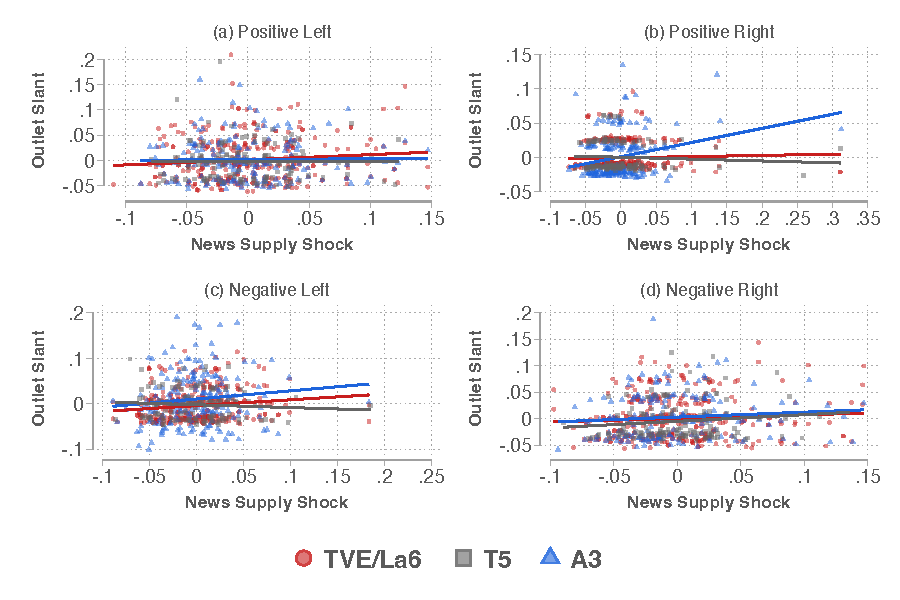
\includegraphics[width=160mm]{figures/fwl_plots_v2}
		\caption*{\small \textit{Note:} The figure shows the added variable plots from the estimation of equation \ref{eq:first_stage}. The x axis represents the news shocks $z_d^k $ and the y axis the corresponding outlet's slant $x_{jd}^k $   . Channels are pooled into left (TVE and La Sexta), middle (Telecinco) and right (A3) for visualization purposes.  }
		\label{fig:fwl}
	\end{figure}
	
	Importantly for the identification strategy, there is variation across outlets in this mechanism. Table \ref{tab:tests}  which shows the F test for equality of coefficients across all outlets and the t-test for equality between right and left outlets. The highest, more significant differences occur for pro-right content.
	
	
	
	\begin{table}[!htbp]
		\centering
	

		\caption{F and t-tests for Regression Coefficients}
		\begin{tabular}{lcccc}
			\hline
			Characteristic & F-test  & F-test p-value & T-test  & T-test p-value \\
			\hline
			$ {L-}$& 2.69 & 0.0686 & 3.51  & 0.0613 \\
			$ {L+}$ & 1.31 & 0.2711 & 1.87  & 0.1715 \\
			$ {R-}$ & 0.42 & 0.6594 & 0.34 & 0.5592 \\
$ {R+}$ & 8.78 & 0.0002 & 17.55  & 0.0000 \\
			\hline
		\end{tabular}
			\caption*{\small \textit{Note:} Summary of F- and T-test results for equality of news variable coefficients across channels. The F-test evaluates overall equality across channels, while the T-test compares the coefficient of the main independent variable between A3 and TVE/La Sexta.}
					\label{tab:tests}
	\end{table}
	

	
		
	
	Accordingly, I use
	$\bigl(z_d^{party+},z_d^{party-},z_d^{political}\bigr)_{party\in\{L,R\}}$
	as instruments for the linear content characteristics.  For the $K$ non-linear parameters governing preference heterogeneity I follow \citet{gandhi2019measuring} and use instruments of the form 
	$\bigl(\hat{x}_{jd}^k-\sum_{l\neq j}\hat{x}_{ld}^k\bigr)^2$,
	where $\hat{x}_{jd}^k$ is the first-stage prediction from~\eqref{eq:first_stage}.
	To identify demographic interactions, I multiply these instruments by the average share of right-wing votes, $\bar y_{mr}\,\hat{x}_{jd}^k$.



	\subsection{Results of the Demand Estimation}
	
	\label{sec:results}
	
	
I present the results of the BLP estimation for the off-campaign and campaign periods in Table \ref{tab:results_blp}. I show the preferred specification with both outlet and day-of-week fixed effects, and standard errors clustered at the regional level. Because the political division in demographics is only between left- and right-leaning viewers, the \(\beta\)s represent the mean tastes of left-leaning viewers and the \(\pi\)s are deviations for right-leaning audiences.


Most of the heterogeneity is captured by the demographics (i.e ideology).  The estimated taste-dispersion parameters (\(\sigma\)s) are small and very imprecise. The high standard errors on these coefficients come by construction. The identification on the random-coefficients relies on variation across markets in the choice set, which is null in my case given the same products are present across region-dates. These low values of heterogeneity naturally link to the similar results that I obtain under the multinomial logit specification shown in Table \ref{tab:logit}. 
 
  In order to give better interpretation of the content-taste parameters I present the mean own elasticities for both the off-campaign and campaign periods.   Given that increasing the positive relative minutes to a party also implies increasing the overall total minutes on politics, I compute the elasticity for the $k$th characteristic as: 

%The pre-campaign estimates reveal four main facts. First, left-leaning audiences display a strong and precisely estimated mean taste for political stories (\(\beta^{political}>0\)). Second, left-wing viewers are pulled by negative tone on both blocs, with the effect much stronger and significant when the right bloc is the target (\(\beta^{R-}>0\)), while positive-toned stories are, on average, unattractive. Third, estimated taste-dispersion parameters (\(\sigma\)s) are small and very imprecise, which is unsurprising given that random-coefficient identification is weak when the set of products is fixed across markets \citep{berry_haile_econometrica}\footnote{These low values of heterogeneity naturally link to the similar results that I obtain under the plain logit specification shown in Table \ref{tab:logit}.}. Fourth, ideology–content interactions are generally noisy; the main signal is that right-leaning viewers place a lower value on generic political coverage than left-leaning viewers (\(\pi^{political}<0\)). 

%During the campaign window, the average taste of left audiences for political coverage turns negative (\(\beta^{political}<0\)), consistent with saturation once the race is underway. Framing now matters sharply: viewers reward positive stories about the left and negative stories about the right while penalizing the opposite frames, implying an aggregate tilt toward left-leaning parties (\(\beta^{L+}>0\), \(\beta^{R-}>0\), \(\beta^{R+}<0\), \(\beta^{L-}<0\)). Ideology interactions reveal marked polarization, with significant taste differences between right and left viewers. Right-leaning viewers now strongly seek favorable coverage of their own side and avoid negative stories about it (large opposing signs on \(\pi^{R+}\) and \(\pi^{R-}\)), dislike positive coverage of the left (\(\pi^{L+}<0\)), and demand negative coverage of the left (\(\pi^{L-}>0\)), indicating that out-group animosity is an important driver of viewing during the campaign.

	
%My results are consistent with \cite{Peterson2017Echo}, who found that partisans gravitate toward like-minded political content  during the 2016 U.S. presidential campaign. 


	
	
	

	
	
	\begin{comment}
		content...

	I present the results of the BLP estimation for the pre-campaign and campaign periods in Table \ref{tab:results_blp}. I show the preferred specification with outlet and day-of-week fixed effects and standard errors clustered at the regional level.
	
	The pre-campaign estimates reveal four main facts. First, there is a strong, statistically precise mean taste for stories about national politics in left audiences ($\beta^{political}$), indicating that political coverage per se draws audience attention before the campaign begins. Second, conditional on this baseline, viewers demand a negative tone toward both parties, but the pull is considerably stronger when the right-wing bloc is the target, whereas positive-toned stories are, on average, unattractive. Third, there is no sizable dispersion in the taste parameters captured by the estimated $\sigma$. This is expected, as identification of these parameters requires exogenous changes in the choice sets \citep{berry_haile_econometrica}, which do not apply in my market setup (i.e there are always the same amount of channels). Fourth, the ideology–content interaction terms are small and imprecise, so the heterogeneity cannot be explained by viewers’ ideology.
	
	During the campaign window, the same specification paints a markedly different picture. The average taste for political coverage becomes negative, suggesting that left audiences experience saturation once the race begins. Preferences reverse and intensify: viewers now reward positive stories about the left and negative stories about the right while penalising the opposite frames, producing an aggregate tilt toward left-leaning parties. Ideology–content interactions, however, reveal stark polarisation. Right-wing audiences actively seek favourable coverage of their own side and avoid negative stories about it, yet the dominant force is out-group animosity: they exhibit a particularly strong demand for negative coverage of the opposition. This pattern is consistent with \emph{affective polarisation} and echoes evidence from the United States showing that exposure to presidential campaigns makes partisans increasingly hostile toward their opponents \citep{Peterson2017Echo}.
		\end{comment}
	
	
	
	

	\begin{table}[!htbp]
					\caption{BLP Estimation Results with Standard Errors}
					\label{tab:results_blp}
		\centering
		\begin{threeparttable}
			\begin{tabular}{lccc}
				\hline
				\textbf{Coefficient} & \textbf{Parameter} & \textbf{Estimate} & \textbf{Std. Error} \\
				\hline
				\multicolumn{4}{c}{Pre-campaign} \\
				\hline
				\hline
				Positive Left & $\beta^{L+}$ & -16.90 & (11.73) \\
				Positive Right & $\beta^{R+}$ & -25.53 & (31.03) \\
				Negative Left & $\beta^{L-}$ & 28.29 & (25.89) \\
				Negative Right & $\beta^{R-}$ & 56.44** & (28.45) \\
				Political & $\beta^{political}$ & 11.49*** & (4.28) \\
				Weather & $\gamma$ & 0.00 & (0.03) \\
				\hline
				Positive Left & $\sigma^{L+}$ & 0.44 & (296.90) \\
				Positive Right & $\sigma^{R+}$ & 0.68 & (715.26) \\
				Negative Left & $\sigma^{L-}$ & 12.64 & (8.68) \\
				Negative Right & $\sigma^{R-}$ & 21.99 & (13.83) \\
				Political & $\sigma^{political}$ & 0.00 & (46.79) \\
				\hline
				Right-Wing $\times$  Positive Left & $\pi^{L+}$ & 46.26 & (48.70) \\
				Right-Wing $\times$  Positive Right & $\pi^{R+}$ & 77.81 & (95.92) \\
				Right-Wing $\times$  Negative Left & $\pi^{L-}$ & -70.09 & (57.97) \\
				Right-Wing $\times$  Negative Right & $\pi^{R-}$ & -103.71 & (97.76) \\
				Right-Wing $\times$  Political & $\pi^{political}$ & -25.17** & (12.59) \\
				\hline
				\hline
				\multicolumn{4}{c}{Campaign} \\
				\hline
				\hline
				Positive Left & $\beta^{L+}$ & 134.16** & (65.57) \\
				Positive Right & $\beta^{R+}$ & -129.79*** & (48.43) \\
				Negative Left & $\beta^{L-}$ & -104.84** & (41.32) \\
				Negative Right & $\beta^{R-}$ & 92.62** & (41.63) \\
				Political & $\beta^{political}$ & -6.43** & (3.26) \\
				Weather & $\gamma$ & 0.00 & (0.01) \\
				\hline
				Positive Left & $\sigma^{L+}$ & 0.00 & (320.36) \\
				Positive Right & $\sigma^{R+}$ & 19.25* & (10.89) \\
				Negative Left & $\sigma^{L-}$ & 0.00 & (134.33) \\
				Negative Right & $\sigma^{R-}$ & 0.02 & (73.18) \\
				Political & $\sigma^{political}$ & 0.00 & (19.55) \\
				\hline
				Right-Wing $\times$  Positive Left & $\pi^{L+}$ & -421.99** & (176.15) \\
				Right-Wing $\times$  Positive Right & $\pi^{R+}$ & 334.94*** & (127.41) \\
				Right-Wing $\times$  Negative Left & $\pi^{L-}$ & 288.65** & (116.22) \\
				Right-Wing $\times$  Negative Right & $\pi^{R-}$ & -280.33*** & (104.44) \\
				Right-Wing $\times$  Political & $\pi^{political}$ & 19.34** & (8.93) \\
				\hline
				\hline
			\end{tabular}

			\begin{tablenotes}
				\small
				\item \footnotesize{The table shows the results of the BLP estimation of model \ref{eq:utility}. The estimations are divided into the off-campaign and campaign period. Both day-of-the-week and outlet fixed effects are included. Standard errors are clustered at the region level. The total number of observations are $N_{campaign}=2307$ and  $N_{off-campaign}=6604$.}
			\end{tablenotes}
		\end{threeparttable}
	\end{table}
	
	

	

	
	

	
	
	
	
	\begin{comment}
	
	\begin{table}[ht]
		\centering
		\begin{threeparttable}
			\begin{tabular}{lccc}
				\hline
				\textbf{Coefficient} & \textbf{Parameter} & \textbf{Estimate} & \textbf{Std. Error} \\
				\hline
				\hline
				\multicolumn{4}{c}{{Pre-campaign}} \\
				\hline
				\hline
				Positive Left & $\sigma^{L+}$ & 7.04 & (21.28) \\
				Positive Right & $\sigma^{R+}$ & 23.82 & (20.06) \\
				Negative Left & $\sigma^{L-}$ & 3.85 & (11.56) \\
				Negative Right & $\sigma^{R-}$ & 25.42*** & (5.01) \\
				Political & $\sigma^{\text{political}}$ & 3.47 & (7.58) \\
				\hline
				Right-Wing $\times$ Positive Left & $\pi^{L+}$ & 21.75 & (16.78) \\
				Right-Wing $\times$ Positive Right & $\pi^{R+}$ & 35.74 & (43.73) \\
				Right-Wing $\times$ Negative Left & $\pi^{L-}$ & -48.27 & (33.58) \\
				Right-Wing $\times$ Negative Right & $\pi^{R-}$ & -63.86 & (48.13) \\
				Right-Wing $\times$ Political & $\pi^{\text{political}}$ & -13.89 & (12.77) \\
				\hline
				Positive Left & $\beta^{L+}$ & -10.88 & (7.41) \\
				Positive Right & $\beta^{R+}$ & -18.19 & (23.08) \\
				Negative Left & $\beta^{L-}$ & 14.41 & (12.51) \\
				Negative Right & $\beta^{R-}$ & 43.11*** & (16.62) \\
				Political & $\beta^{\text{political}}$ & 4.73 & (5.41) \\
				Weather & $\gamma$ & 0.01 & (0.01) \\
				\hline
				\hline
				\multicolumn{4}{c}{{Campaign}} \\
				\hline
				\hline
				Positive Left & $\sigma^{L+}$ & 1.26 & (145.13) \\
				Positive Right & $\sigma^{R+}$ & 33.40 & (42.70) \\
				Negative Left & $\sigma^{L-}$ & 0.38 & (218.79) \\
				Negative Right & $\sigma^{R-}$ & 0.54 & (226.19) \\
				Political & $\sigma^{\text{political}}$ & 2.92*** & (0.90) \\
				\hline
				Right-Wing $\times$ Positive Left & $\pi^{L+}$ & -708.11** & (299.27) \\
				Right-Wing $\times$ Positive Right & $\pi^{R+}$ & 508.87*** & (172.30) \\
				Right-Wing $\times$ Negative Left & $\pi^{L-}$ & 413.36*** & (147.90) \\
				Right-Wing $\times$ Negative Right & $\pi^{R-}$ & -455.86** & (178.69) \\
				Right-Wing $\times$ Political & $\pi^{\text{political}}$ & 27.60** & (12.62) \\
				\hline
				Positive Left & $\beta^{L+}$ & 217.09*** & (76.90) \\
				Positive Right & $\beta^{R+}$ & -190.52** & (89.31) \\
				Negative Left & $\beta^{L-}$ & -145.58*** & (48.63) \\
				Negative Right & $\beta^{R-}$ & 147.49*** & (52.60) \\
				Political & $\beta^{\text{political}}$ & -10.80** & (4.89) \\
				Weather & $\gamma$ & 0.04 & (0.03) \\
				\hline
				\hline
			\end{tabular}
			\caption{BLP Estimation Results with Standard Errors}
							\label{tab:results_blp_updated}
			\begin{tablenotes}
				\small
				\item \footnotesize{The table shows the results of the BLP estimation of model \ref{eq:utility}. The estimations are divided in the pre-campaign and campaign period. Both day of the week and outlet fixed effects are included. Standard errors are clustered at the region level. The total number of observations is $N_{campaign}=2307$ and $N_{pre\_campaign}=6604$.}
			\end{tablenotes}
		\end{threeparttable}

	\end{table}
	
	\end{comment}
	
	
	%\subsubsection{Elasticities}
	
	%I present the mean own elasticities for both the off-campaign and campaign periods.   Given that increasing the positive relative minutes to a party also implies increasing the overall total minutes on politics, I compute the elasticity for the $k$th characteristic as: 
	
	\begin{equation}\label{eq:elasticities}
		\begin{aligned}
			& \bar{\epsilon}^k= \frac{1}{J\times R \times D}\sum_{j}\sum_{r} \sum_{d} \left(\frac{\partial s_{jrd}}{\partial x_{jt}^k} +  \frac{\partial s_{jrd}}{\partial x_{jt}^{political}} \right) \frac{x_{jd}^k}{s_{jrd}}    \quad \forall k \in \{R+,R-,L+,L-\}
		\end{aligned}
	\end{equation}             
	
	
	
	Results of the mean elasticities are shown in Appendix Table \ref{tab:elasticities0}.	Both left and right parties were almost equally liked during off-campaign. An increase of 1 percent in net tone ($\bar{\epsilon}^{\text{party}+}-\bar{\epsilon}^{\text{party}-}$) towards right (left) results in drops of 0.98 (1.00) percentage points in audience share; corresponding to a decrease of nearly 13,000 viewers.\footnote{A 1 pp increase in airtime on characteristic $k$ changes audience share by $\Delta S = S \times \tfrac{\epsilon}{100}$. Given an average total audience of $\bar{L}$, the level change in viewers is $\Delta V = \Delta S \times \bar{L}$. Since 1 pp of airtime corresponds to $0.01\,\bar{T}$ minutes (where $\bar{T}$ is the average broadcast length), $\tfrac{\Delta V}{\Delta t} = \bigl(S \times \tfrac{\epsilon}{100} \times \bar{L}\bigr) \times \tfrac{1}{0.01\,\bar{T}}$ gives the change in viewers per extra minute of coverage.} This is consistent with a taste for scandals or entertainment like type of political content, which is more likely to happen off-campaigns. During the campaign, audiences remain averse to right-leaning tone—though less so, with only a 0.60 pp loss—but the effect of net left-leaning tone flips to 0.09 pp increase (867 viewers).
	
	
	To see the extent of polarization in news consumption, I  compute elasticities for right and left markets separately. I define a “right market” as any region whose mean intention-to-vote $\bar{y}_r$ lies above the median. 
	 Figure~\ref{fig:elasticities_campaign} plots the estimated elasticities for the campaign\footnote{Table~\ref{tab:elasticities} and 	 Figure~\ref{fig:elasticities_pre} show full results also for the off-campaign period. } for left markets (panel a) and right markets (panel b).	Polarization becomes now evident. Left viewers present negative taste to content that harms their party and positive taste for that benefits it. The analogous pattern is present in the taste of right wing viewers. 
	 
	  For example, a 1 pp increase in negative-right tone during the campaign is associated with a net loss of 8,015 total viewers in right markets relative to  the off-campaign period.
	
	

	
	\begin{figure}[!htbp]
		\centering
		\caption{Estimated Elasticities for Left and Right markets during Campaign}
\label{fig:elasticities_campaign}
		\vspace{0.5em} % space between caption and figures
		
		\begin{minipage}{0.45\textwidth}
			\centering
			(a) Left Markets\\
			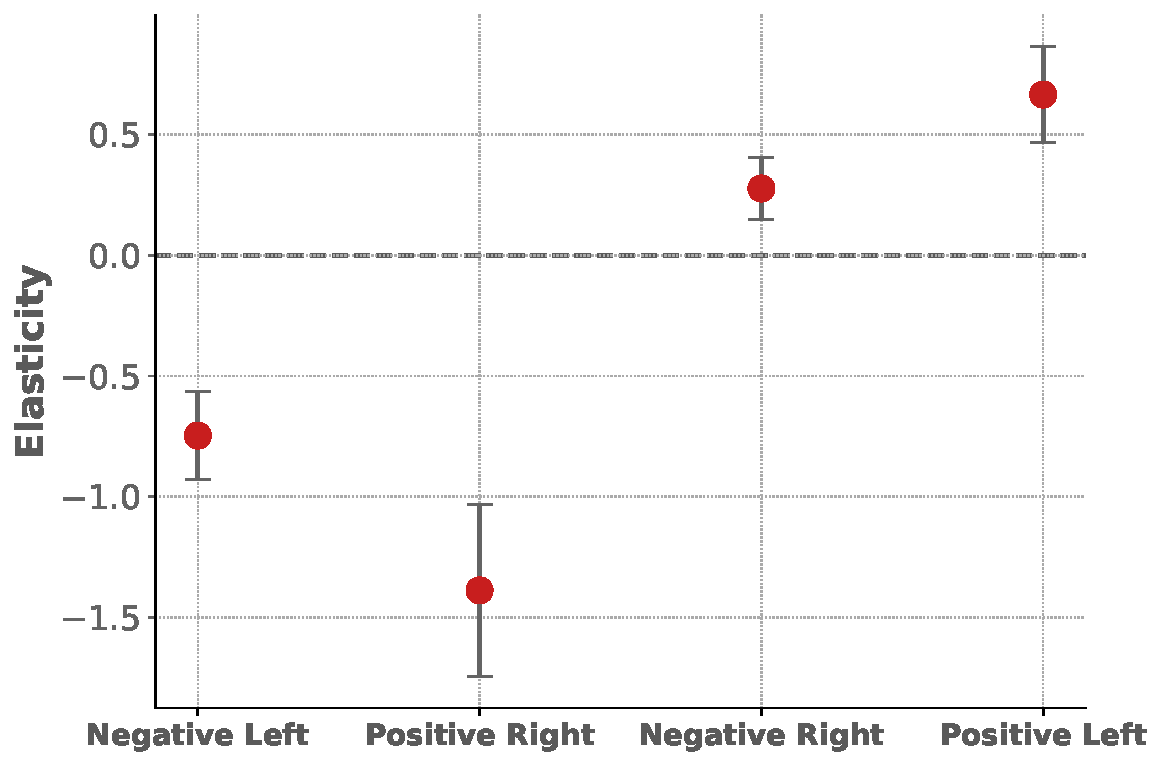
\includegraphics[width=\linewidth]{figures/elasticities_left_campaign}
			%		\label{fig:2figsA}
		\end{minipage}
		\hfill
		\begin{minipage}{0.45\textwidth}
			\centering
			\vspace{1.5em}
			(b) Right Markets \\
						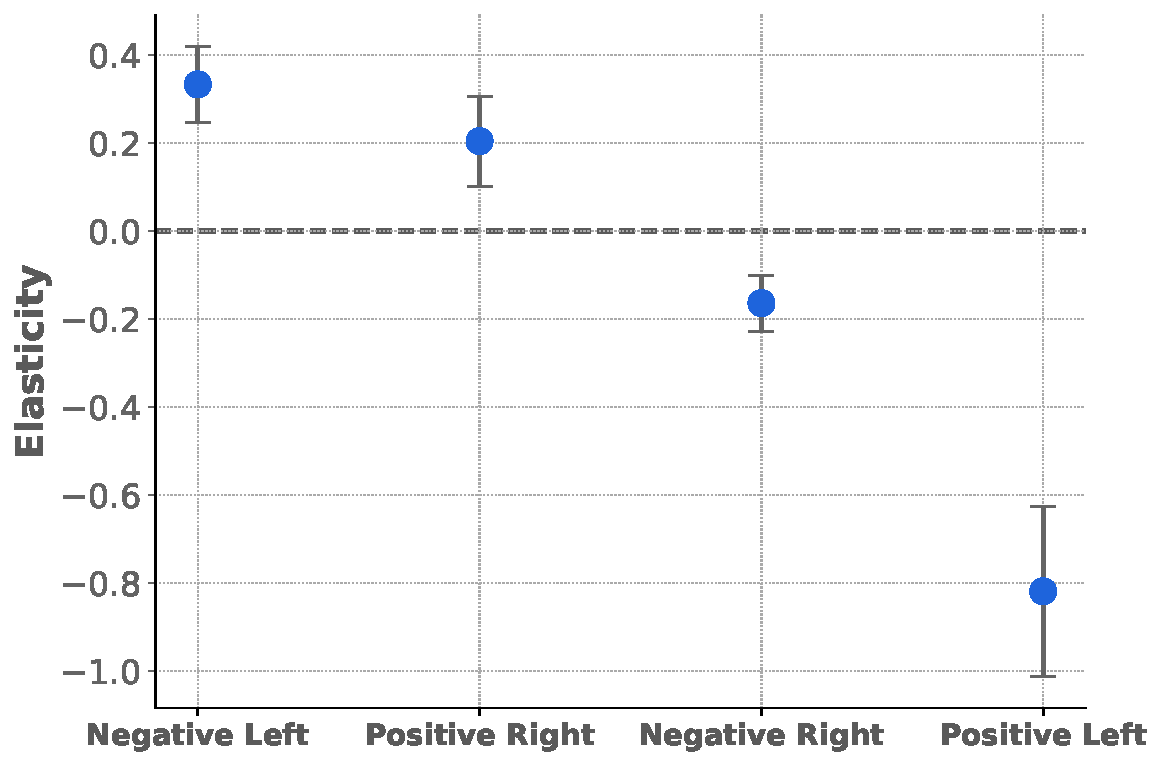
\includegraphics[width=\linewidth]{figures/elasticities_right_campaign}
			\label{fig:2figsA}
		\end{minipage}
		
		\vspace{0.5em} % space between figures and note
		
		\captionsetup{justification=justified}
		\caption*{\textit{Note:} \small Each panel shows estimated mean own elasticities for consumer responses  as described in equation \ref{eq:elasticities} during the campaign period. Panel (a) reports results for the left-leaning markets, while Panel (b) shows the results for the right-leaning markets. Right markets are defined as regions with proportion of right wing voters above the median. Whiskers represent the $95\%$ confidence intervals of the mean across markets.}
						
	\end{figure}
	

	
%These results are consistent with \cite{Peterson2017Echo}, who found that partisans gravitate toward like-minded political content  during the 2016 U.S. presidential campaign. Specifically, by decomposing the different-party tone combinations, I also match the \textit{affective} type of polarization, where the negative taste towards favorable content on the opposition dominates. 





\begin{comment}
content...

\begin{figure}[!htbp]
	\centering
	\caption{Estimated Elasticities for Right and Left markets, Pre-campaign and Campaign}
	
	\vspace{0.5em} % space between caption and figures
	
	\begin{minipage}{0.45\textwidth}
		\centering
		\textbf{(a)} Pre-campaign\\
		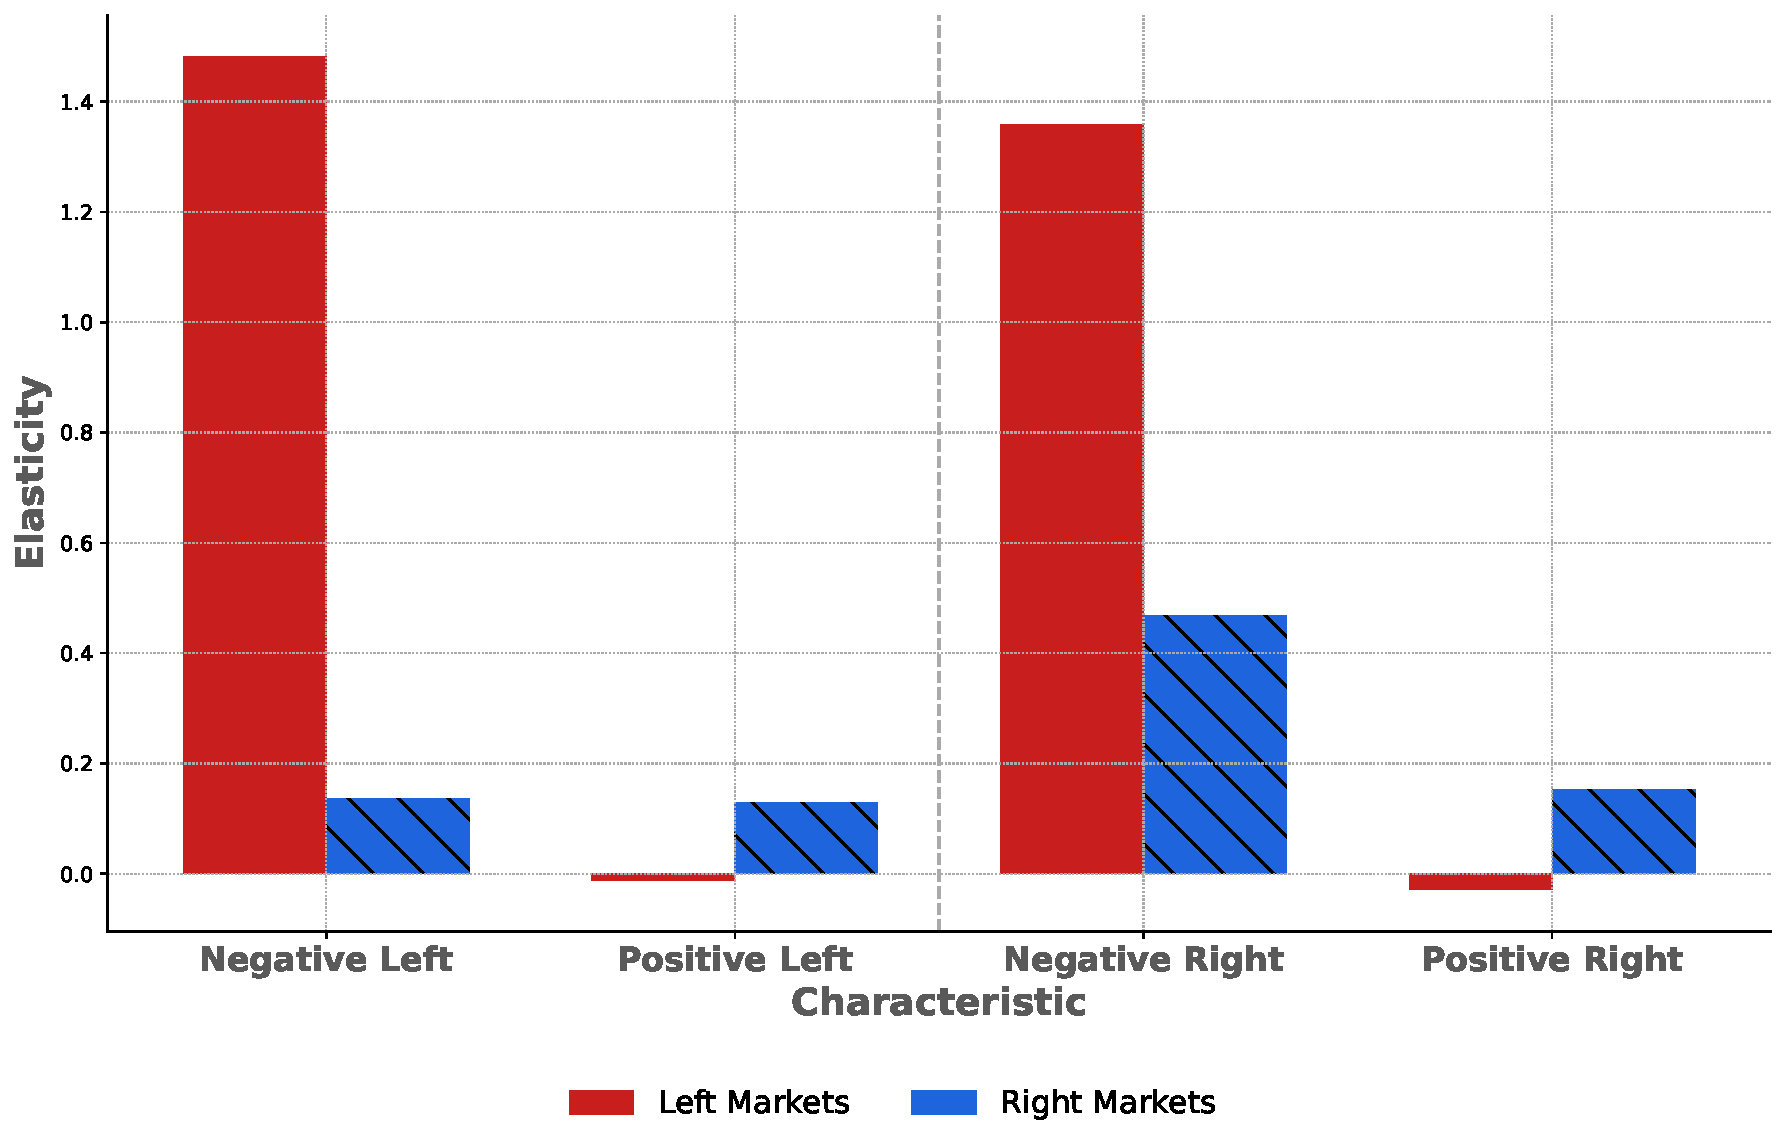
\includegraphics[width=\linewidth]{figures/elasticities_pre_campaign}
%		\label{fig:2figsA}
	\end{minipage}
	\hfill
	\begin{minipage}{0.45\textwidth}
		\centering
				\vspace{1.5em}
		\textbf{(b)} Campaign\\

		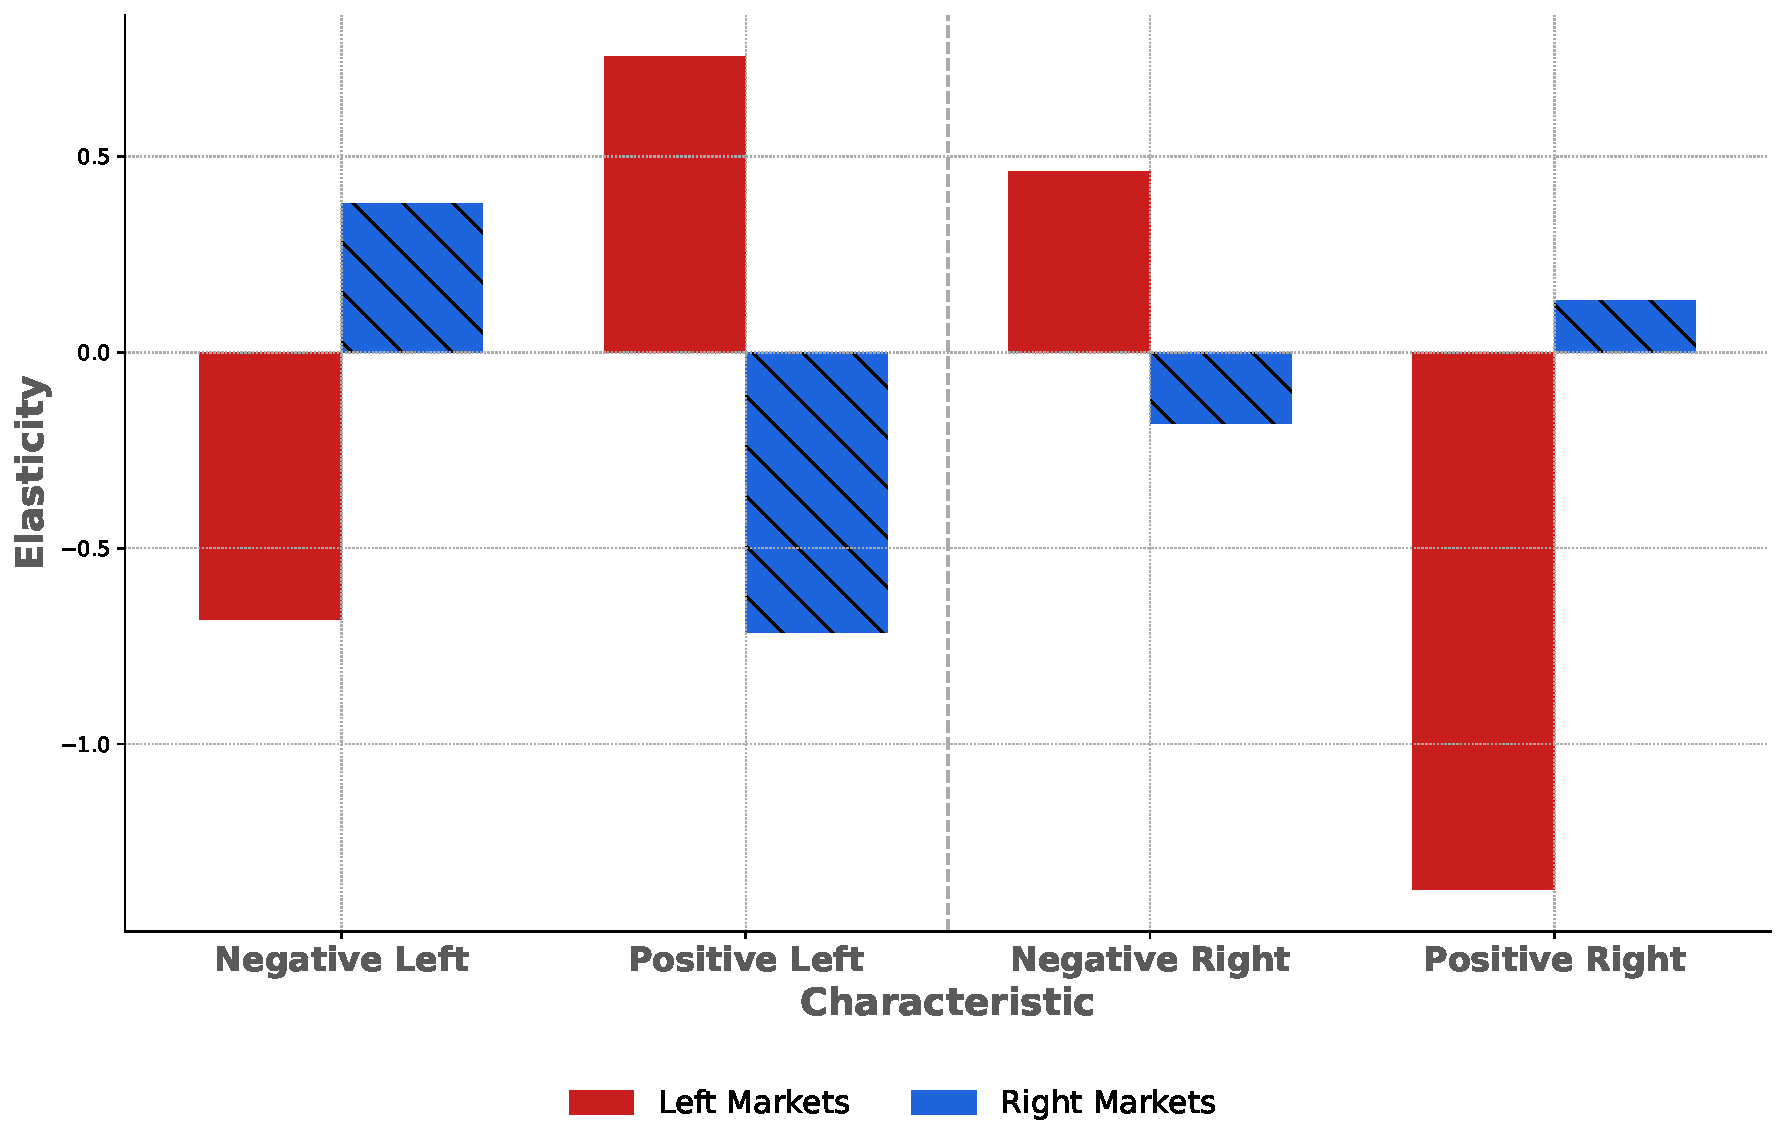
\includegraphics[width=\linewidth]{figures/elasticities_campaign}
		\label{fig:2figsA}
	\end{minipage}
	
	\vspace{0.5em} % space between figures and note
	
	\captionsetup{justification=justified}
	\caption*{\textit{Note:} \small Each panel shows estimated mean own elasticities for consumer responses in right- and left-leaning markets as described in equation \ref{eq:elasticities}. Panel (a) reports results for the pre-campaign period, while Panel (b) covers the campaign period.}
\end{figure}



\end{comment}




%In order to replicate the outlets' positions shown in Figure \ref{fig:channel_ideology_lines}; I do the analogous comparison ranking them according to their estimated demand elasticities. Figure \ref{fig:channel_ideology_lines2} on the appendix shows the comparison. Panel a) ranks channels in the -1,1 segment according to the campaign elasticities. Panel (b) shows their positions for the same period according to their slant. Both rankings are consistent and the relative scores of the middle channels are similar indicating the consistent equilibrium between supply and demand estimates. Still, differences arise since channels face costs of producing content. In the next section I estimate the supply problem of the channels given demand estimates. 





	\subsection{Demand for News and Political Polarization}
	
	
	

Does the polarization in media consumption link to electoral attitudes?  I show correlational evidence between political and media polarization from my demand estimates. As in \cite{martin2017}, I compute  the Esteban-Ray (ER) polarization index \citep{esteban} using the intention to vote by region as:

\begin{equation}
	ER_{rm}  =	 \sum_{p}   \sum_{q}
	s_{prm}^{\,1+\alpha}\,s_{qrm} \times 1,
		\label{eq:er}
\end{equation}

where $s_{pm}$ is the share of intention to vote for party $p\in \{L,R\}$  on month $m$ and I set the standard value $\alpha=1.5$. Since there are only two blocks, the distance between political parties is normalized to one.  Higher values of the index signal a sharper left‑right split in the electorate, i.e., greater political polarization.


I measure affective media polarization as the in-party vs. out-party gap in audience reactions to campaign coverage. Specifically, I calculate the \emph{elasticity gap} between reactions to congenial and uncongenial coverage during the campaign period. For right wing regions, $p(r)=R$, media polarization refers to the difference in taste for negative content on the left versus positive and viceversa: 


\begin{equation}
	MediaPolarization_r  =	\begin{cases}
		\bar{\epsilon}_r^{(L-)}- \bar{\epsilon}_r^{(L+)} \quad if \quad p(r)=R\\
		\bar{\epsilon}_r^{(R-)}- \bar{\epsilon}_r^{(R+)} \quad if \quad p(r)=L
	\end{cases}
		\label{eq:mediapol}
\end{equation}

Because the estimates satisfy
\(\bar{\epsilon}_r^{(L-)}>\bar{\epsilon}_r^{(L+)}\) in right‑leaning regions and
\(\bar{\epsilon}_r^{(R-)}>\bar{\epsilon}_r^{(R+)}\) in left‑leaning ones,
the index in~\eqref{eq:mediapol} is always non‑negative and therefore comparable across regions. Larger values indicate that audiences penalize the out-party more (and/or reward it less) relative to the in-party, consistent with  in-out party evaluation gaps used to measure affective polarization  \citep{IyengarLelkesLevendusky2019Origins}.

I divide regions into \textit{high} and \textit{low} groups according to their media polarization index relative to the median. Figure \ref{fig:er1} plots the smoothed ER index for these two groups over the year before and after the 2023 general election (raw series in Appendix Figure \ref{fig:er}). Solid lines (dashed) denote high- (low-) media-polarized regions.

Regions with high media‑consumption polarization (solid line) consistently show higher political polarization than their low‑polarization counterparts (dashed line)—a ranking that persists even when the series is extended one year before the main sample window. Echoing the demand‑side results, political polarization starts to escalate a month before the formal campaign period: the gap between the two groups first narrows slightly, then widens sharply once the campaign begins.

Between April 2023 and the general election in July 2023, the Esteban–Ray index rises by 0.019 points in high-polarization regions and 0.012 points in low-polarization regions. When scaled by their respective pre-campaign variability, these changes correspond to 3.8 and 5.2 standard deviations, underscoring that the campaign coincided with an unusually abrupt increase in political polarization.

Importantly, the absolute increase is concentrated in high media-polarization regions—those where news consumption was already most segregated—so the observed jump in ideological polarization is essentially generated by the “extreme partisan” audiences. This pattern resonates with studies showing that selective exposure amplifies attitudes among strong partisans \citep{levendusky}, but departs from their observed short-run dynamics. Whereas \citet{levendusky} and \citet{Hernndez2020AffectivePA} document a rebound of polarization back to baseline levels shortly after peak campaign activity, this evidence reveals no such short-run recovery: the increase persists for at least one year after the campaign.




\begin{figure}[!htbp]

	\centering
		\caption{Political and Media Polarization}
	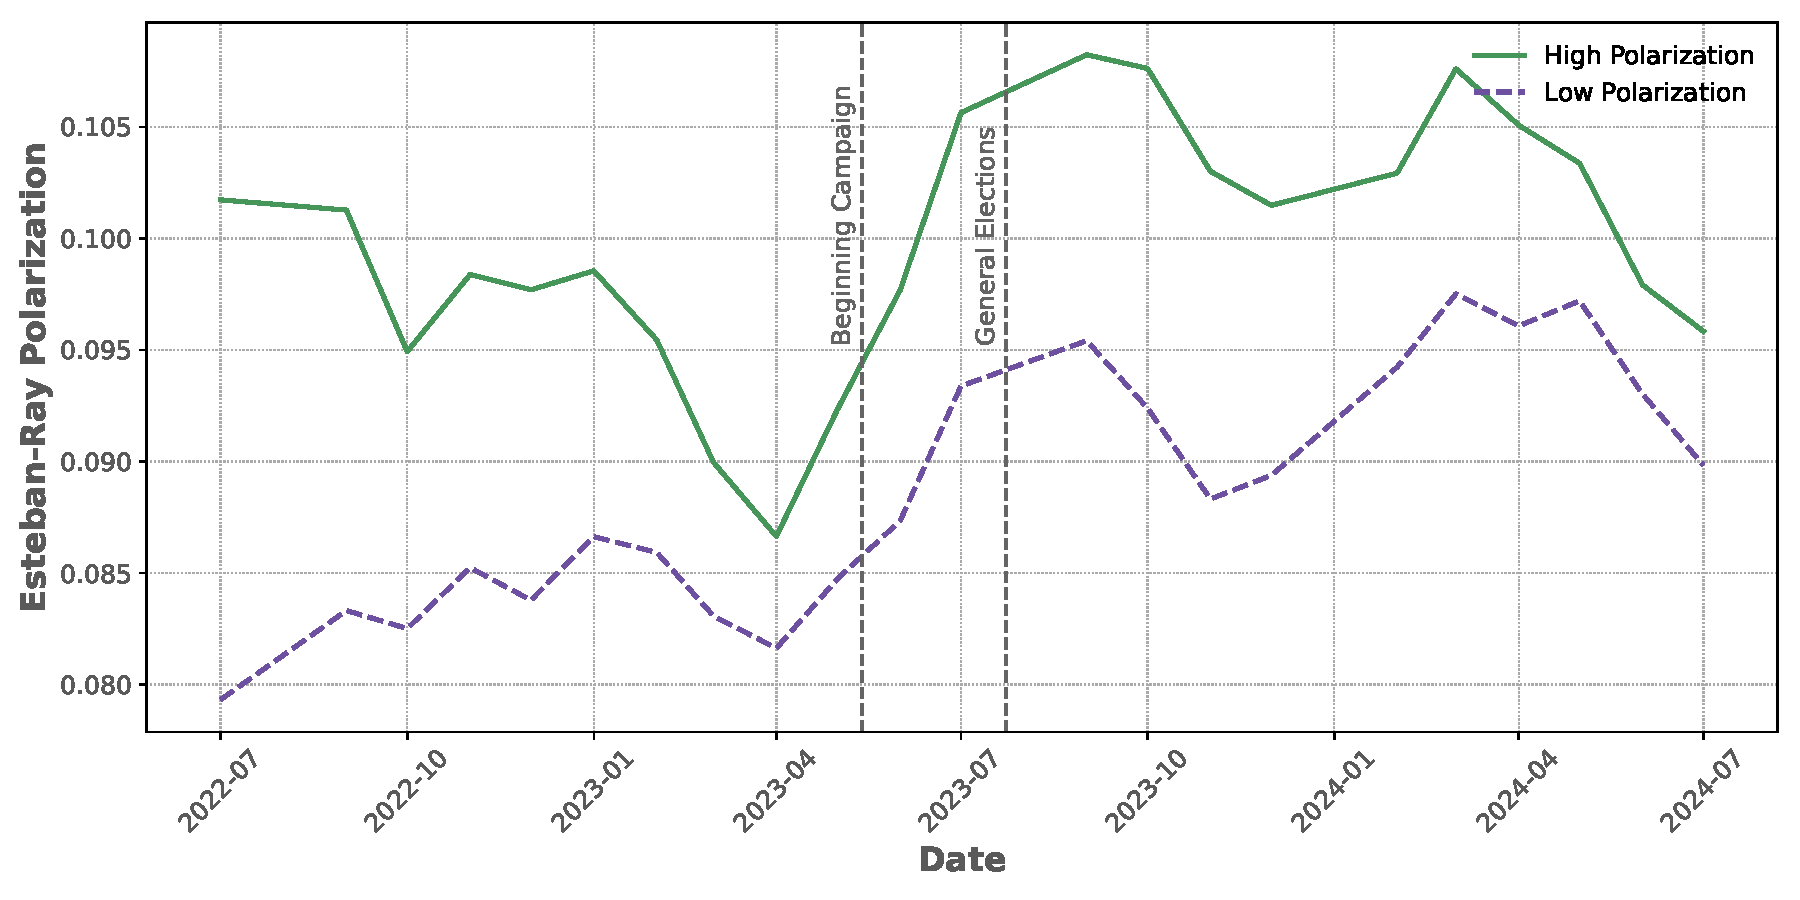
\includegraphics[width=150mm]{figures/er_polarization_stata_group}
				\label{fig:er1}
	\caption*{\textit{Note:} \small The figure shows the mean Esteban-Ray polarization index under a smoothed rolling mean of 3 months computed as in equation \ref{eq:er}.  Solid (dashed) line represents the regions above (below) the median in terms of their media polarization consumption according to index \ref{eq:mediapol}.   }

\end{figure}

\paragraph{Limitations}

To conclude the results section for demand, it is important to discuss some limitations of my analysis.

First, the use of aggregate data cannot rule out selection effects. Campaigns might change audience composition toward news seekers, who have been shown to have asymmetric effects—relative to entertainment seekers—on polarization \citep{levendusky,arceneaux_johnson_2013}. This could lead to an overestimation of preference polarization. 

Second, the link between media and political polarization naturally raises the question of how much of the shift in preferences is driven by changes in ideological polarization. I re-estimate the model in Equation~\ref{eq:utility} using initial (i.e., December) rather than monthly ideology measures; the results are robust. However, this does not mitigate the concern about the potential endogeneity of ideology, which remains a limitation of this paper. Future work might address this concern using individual panel data or by allowing more flexible dynamics between ideology and media consumption, as in \cite{martin2017}.

 



\section{Supply of News}


\label{sec:supply}








The demand estimates in Section~\ref{sec:results} show that viewers react sharply to
partisan tone, especially during the campaign.  This  leads to the complementary question:
How do broadcasters decide which mix of stories and tones to air each day? 
Spanish prime‑time newscasts are produced under tight time constraints, with producers
constantly monitoring real‑time ratings and the incoming news wire.  
The following remark from the News director of one of the channels captures this: 


\begin{quote}
	“Even a news programme is deeply subject to the day-to-day swings of audience share.  
	A drop of half a point when covering a topic can lead us to drop that topic altogether.”
\end{quote}
\hspace*{\fill}–––Vicente Vallés, Director and Presenter, Antena 3 News (2014)\footnote{Source: \url{https://cadenaser.com/ser/2014/12/03/television/1417630810_539829.html}}

Producers therefore aim to maximise the audience handed off to the next slot—despite the bulletin itself carrying no advertising—and fine‑tune slant before each edition.

\subsection{Supply Model}

I capture this behavior with a competitive model of news' slant decisions. Channel $j$ on day $d$ and edition $h\in\{0\text{ (mid-day)},1\text{ (evening)}\}$ solves the following problem:



\begin{equation}\label{eq:payoffs}
	\begin{aligned}
		\max_{\{\mathbf{x}_{jdh}\}}   & \left\{   \sum_{r}\bm{s}_{jrd+1}(\bm{x}_{jdh}, \bm{x}_{-jdh})\frac{L_r}{L} -  \mathcal{C}\left(  \bm{x}_{jdh},\bm{z}_{dh}, \bm{\omega}_{jdh}; \bm{\lambda_j}   \right)    \right\}\\
		s.t.   \quad &   x_{jdh}^{L+} +x_{jdh}^{R+} + x_{jdh}^{L-} + x_{jdh}^{R-} + x_{jdh}^{\emptyset} = x_{jdh}^{political}\\
		& x_{jdh}^k \in [0,1] \quad \forall k
	\end{aligned}
\end{equation} 






where $\bm z_{dh}$ measures the pool of stories available at edition~$h$ and $\bm x_{jdh}$ is the proportion of minutes to each tone category as defined above. 
I parameterize the cost function as:

\begin{equation*}\label{}
	\begin{aligned}
		& \mathcal{C}(x_{jdh}^k,z_{dh}^k,\omega^k_{jdh}; \lambda_j^k )\equiv   \lambda_j^k  \dfrac{(x_{jdh}^k)^2}{z_{dh}^k} + F(\omega^k_{jdh}).
	\end{aligned}
\end{equation*} 

 The $\bm{\lambda_j}$s are a channel-characteristic specific parameters that govern the slope of the production costs. There is unobserved (to the econometrician)  factors other than the stories available; captured by $ F(\omega^k_{jdh})$. By assumption, these unobservables will enter as linear terms in the marginal costs. 

The sign of~$\lambda_j^k$
is theoretically ambiguous ex-ante. On the one hand, $z$ might act as a simple input in any production costs. High availability of stories of a given type will make production easier since the journalist need not do much effort to find them. This will imply $ \lambda>0$. On the other hand, since outlets are news aggregators, having more stories available of a given type might increase the cost of producing them since they would need to process and filter the ones that they prefer. This mechanism is consistent under $ \lambda<0$.

The first-order condition (ignoring the summation constraint for estimation) are
\begin{equation}\label{eq:focs}
	\underbrace{\sum_{r}\frac{\partial s_{jrd+1}}{\partial x_{jdh}^k}\frac{L_r}{L}}_{\equiv g_{jd+1h}^k}=	2\lambda_j^k\frac{x_{jdh}^k}{z_{dh}^k}  +\underbrace{	\eta_{jd}^k+\nu_{jdh}^k}_{\equiv F'(\omega_{jdh}^k)}  \quad \forall(j,k)
\end{equation}


where, for notational simplicity, the derivative for all the tone characteristics also includes the marginal effect on $x^{political}$ but is omitted from the formulation. 

I decompose the unobserved cost factors into 
$\eta_{jd}^k$, a \emph{ day-specific} marginal-cost shock
(e.g.\ a key reporter is on sick leave, satellite link fails, or legal concerns delay a segment),
and $\nu_{jdh}^k$ is transitory noise. 


\subsection{Endogeneity and Identification Strategy}


Because $\eta_{jd}^k$ influences both marginal cost and the share gradient
$g_{jd+1h}^k$ would be biased in a naive regression: $\E[g_{jd+1h}^k\,\eta_{jd}^k]\neq0$.


The key identification strategy lies in the assumption that $\eta_{jd}^k$ is constant within the day. This allows me to rely on variation in news production within day that is only due to new stories coming in between the midday and evening editions that alter production.  

Table \ref{tab:within} shows direct examples of the mechanism on the text. I filter the days with the highest within-day increase in coverage by all channels and report the new stories that entered between midday and evening editions for each content type. For instance, on 29 May 2023, stories criticizing the left pushed evening coverage sharply toward a pro-right tone; on 31 May 2023, stories criticizing the right swung coverage the opposite way. These sudden, within-day shifts in story mix create the variation we use to measure viewers’ taste for like-minded versus opposing content.


To show this variation empirically, I first regress the evening on the midday slant of the stations controlling for outlet fixed-effects. The residuals of these regression are the  variation in the evening programming not explained by the midday slant and channel specific attributes. I then regress these residuals on the news shocks $z$ that enter between those two time slots. Figure \ref{fig:diff} shows the scatter of the regression.  There is a positive association for all content categories. This indicates that entry of new content between midday and night is associated with an increase in editorial production of that content in the evening news' shows. 

\begin{figure}[!htb]
	\caption{Within-day relationship between Editorial Content Share (\(x\)) and News Supply Shock (\(z\)).}
	\centering
	\begin{tabular}{@{}cc@{}}
		% Panel headers row
		\text{(a) Positive Left } &
		\text{(b) Positive Right} \\[0.08em]
		% First row of plots
		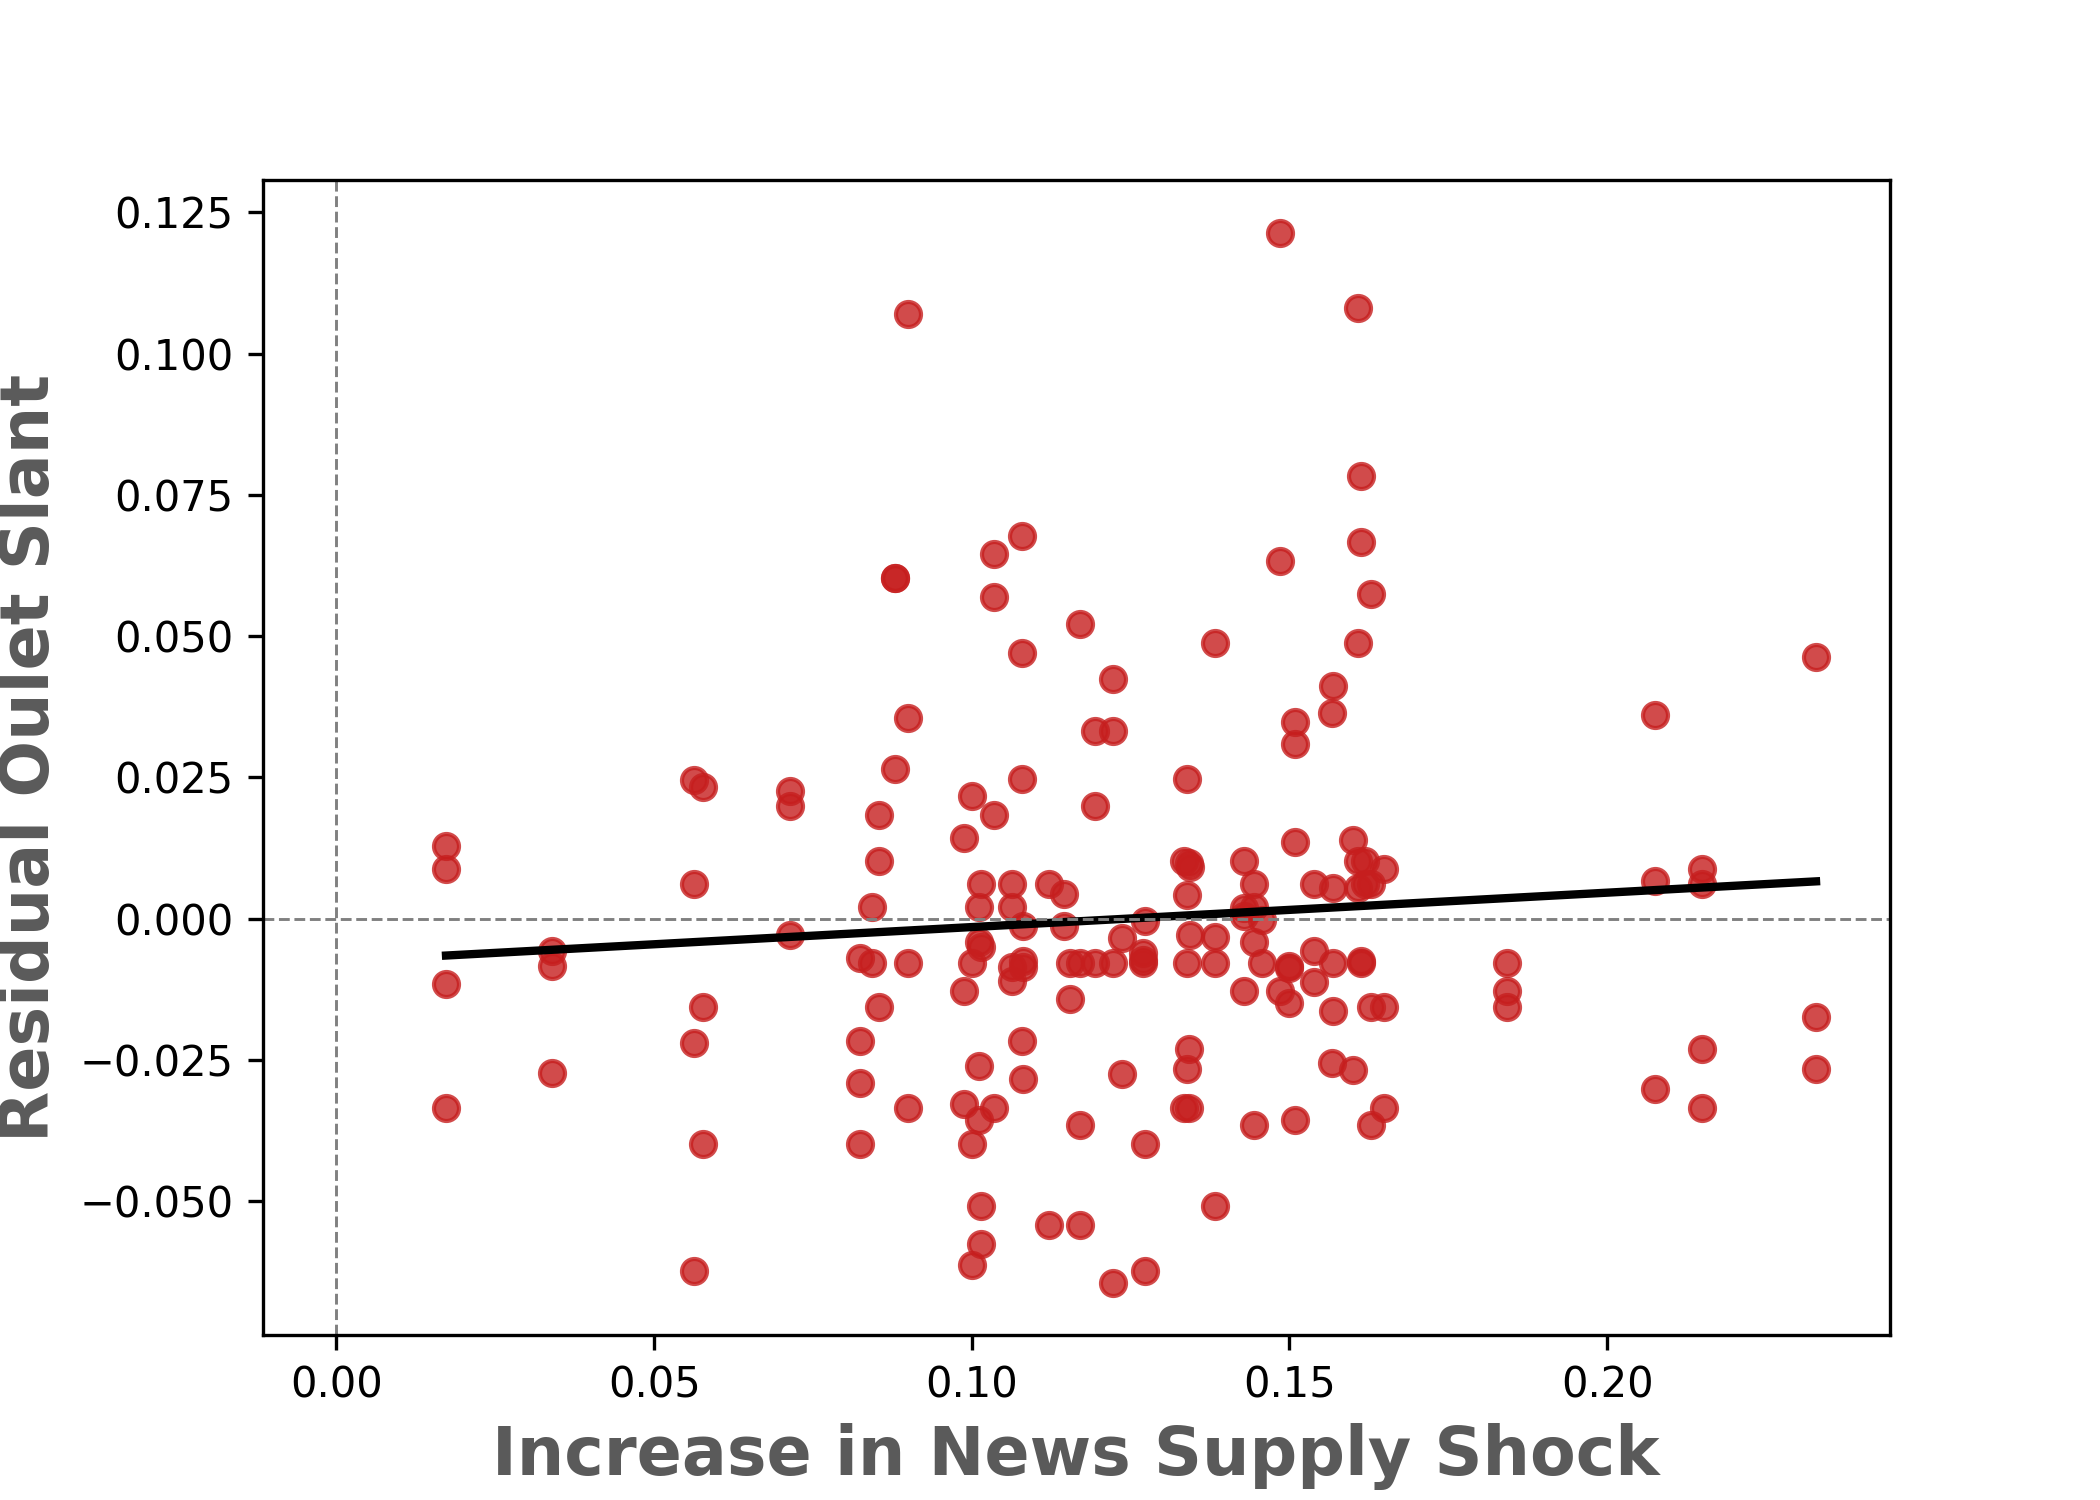
\includegraphics[width=0.45\textwidth]{figures/char_pos_left_residual_v2} &
		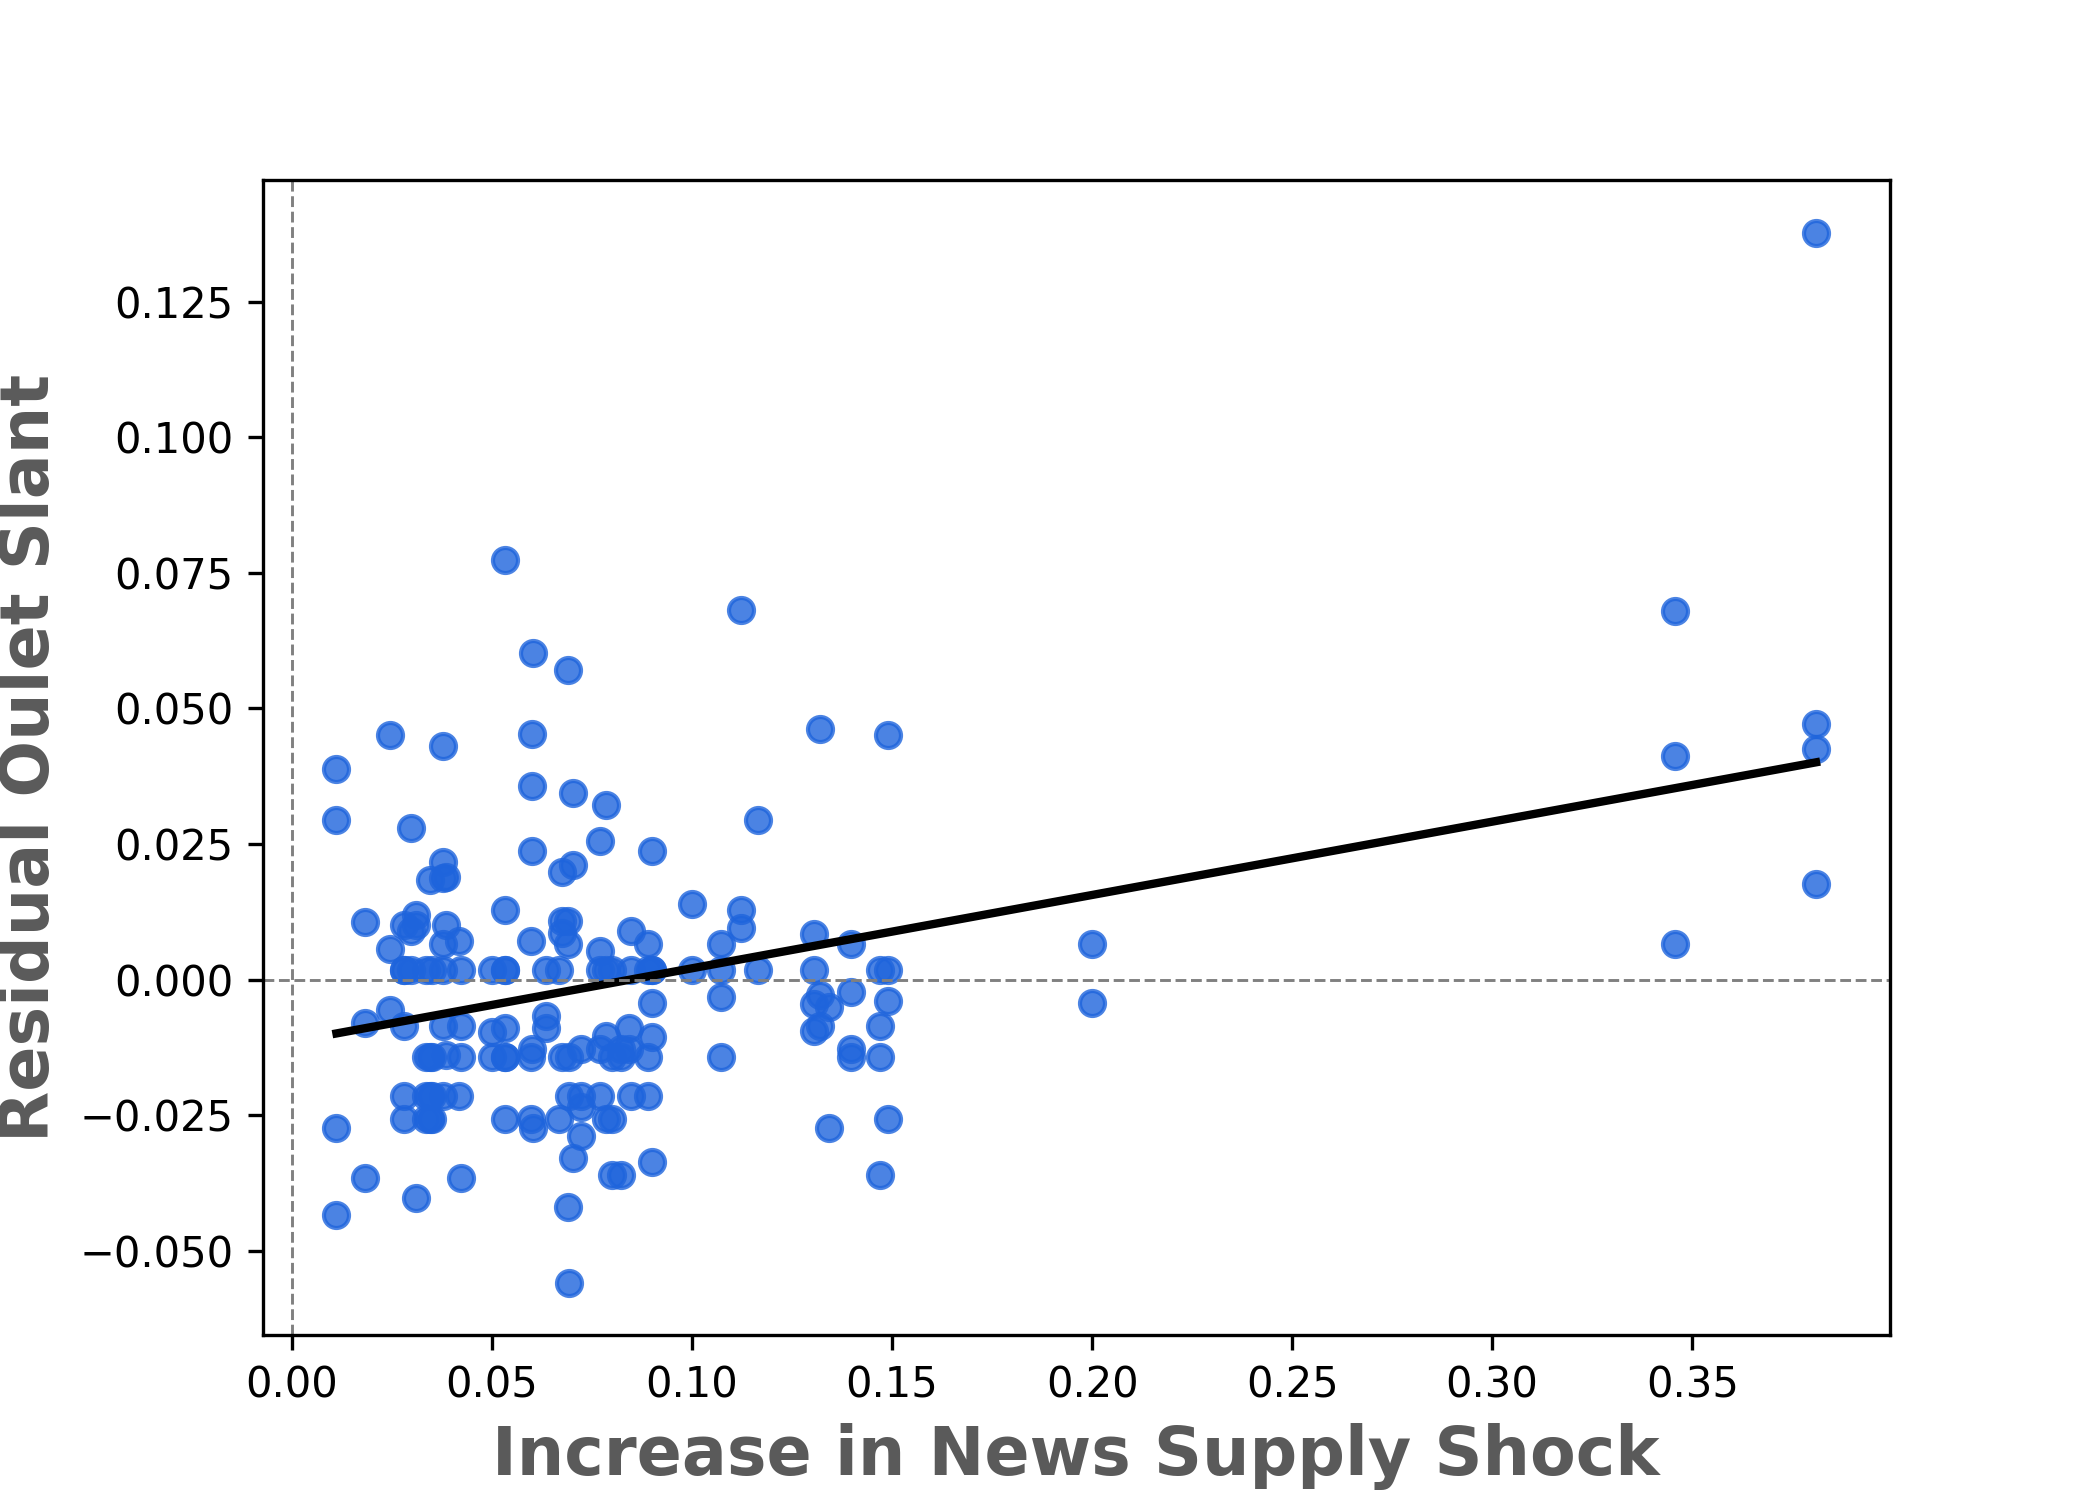
\includegraphics[width=0.45\textwidth]{figures/char_pos_right_residual_v2} \\[1em]
		% Panel headers row
		\text{(c) Negative Left} &
		\text{(d) Negative Right} \\[0.08em]
		% Second row of plots
		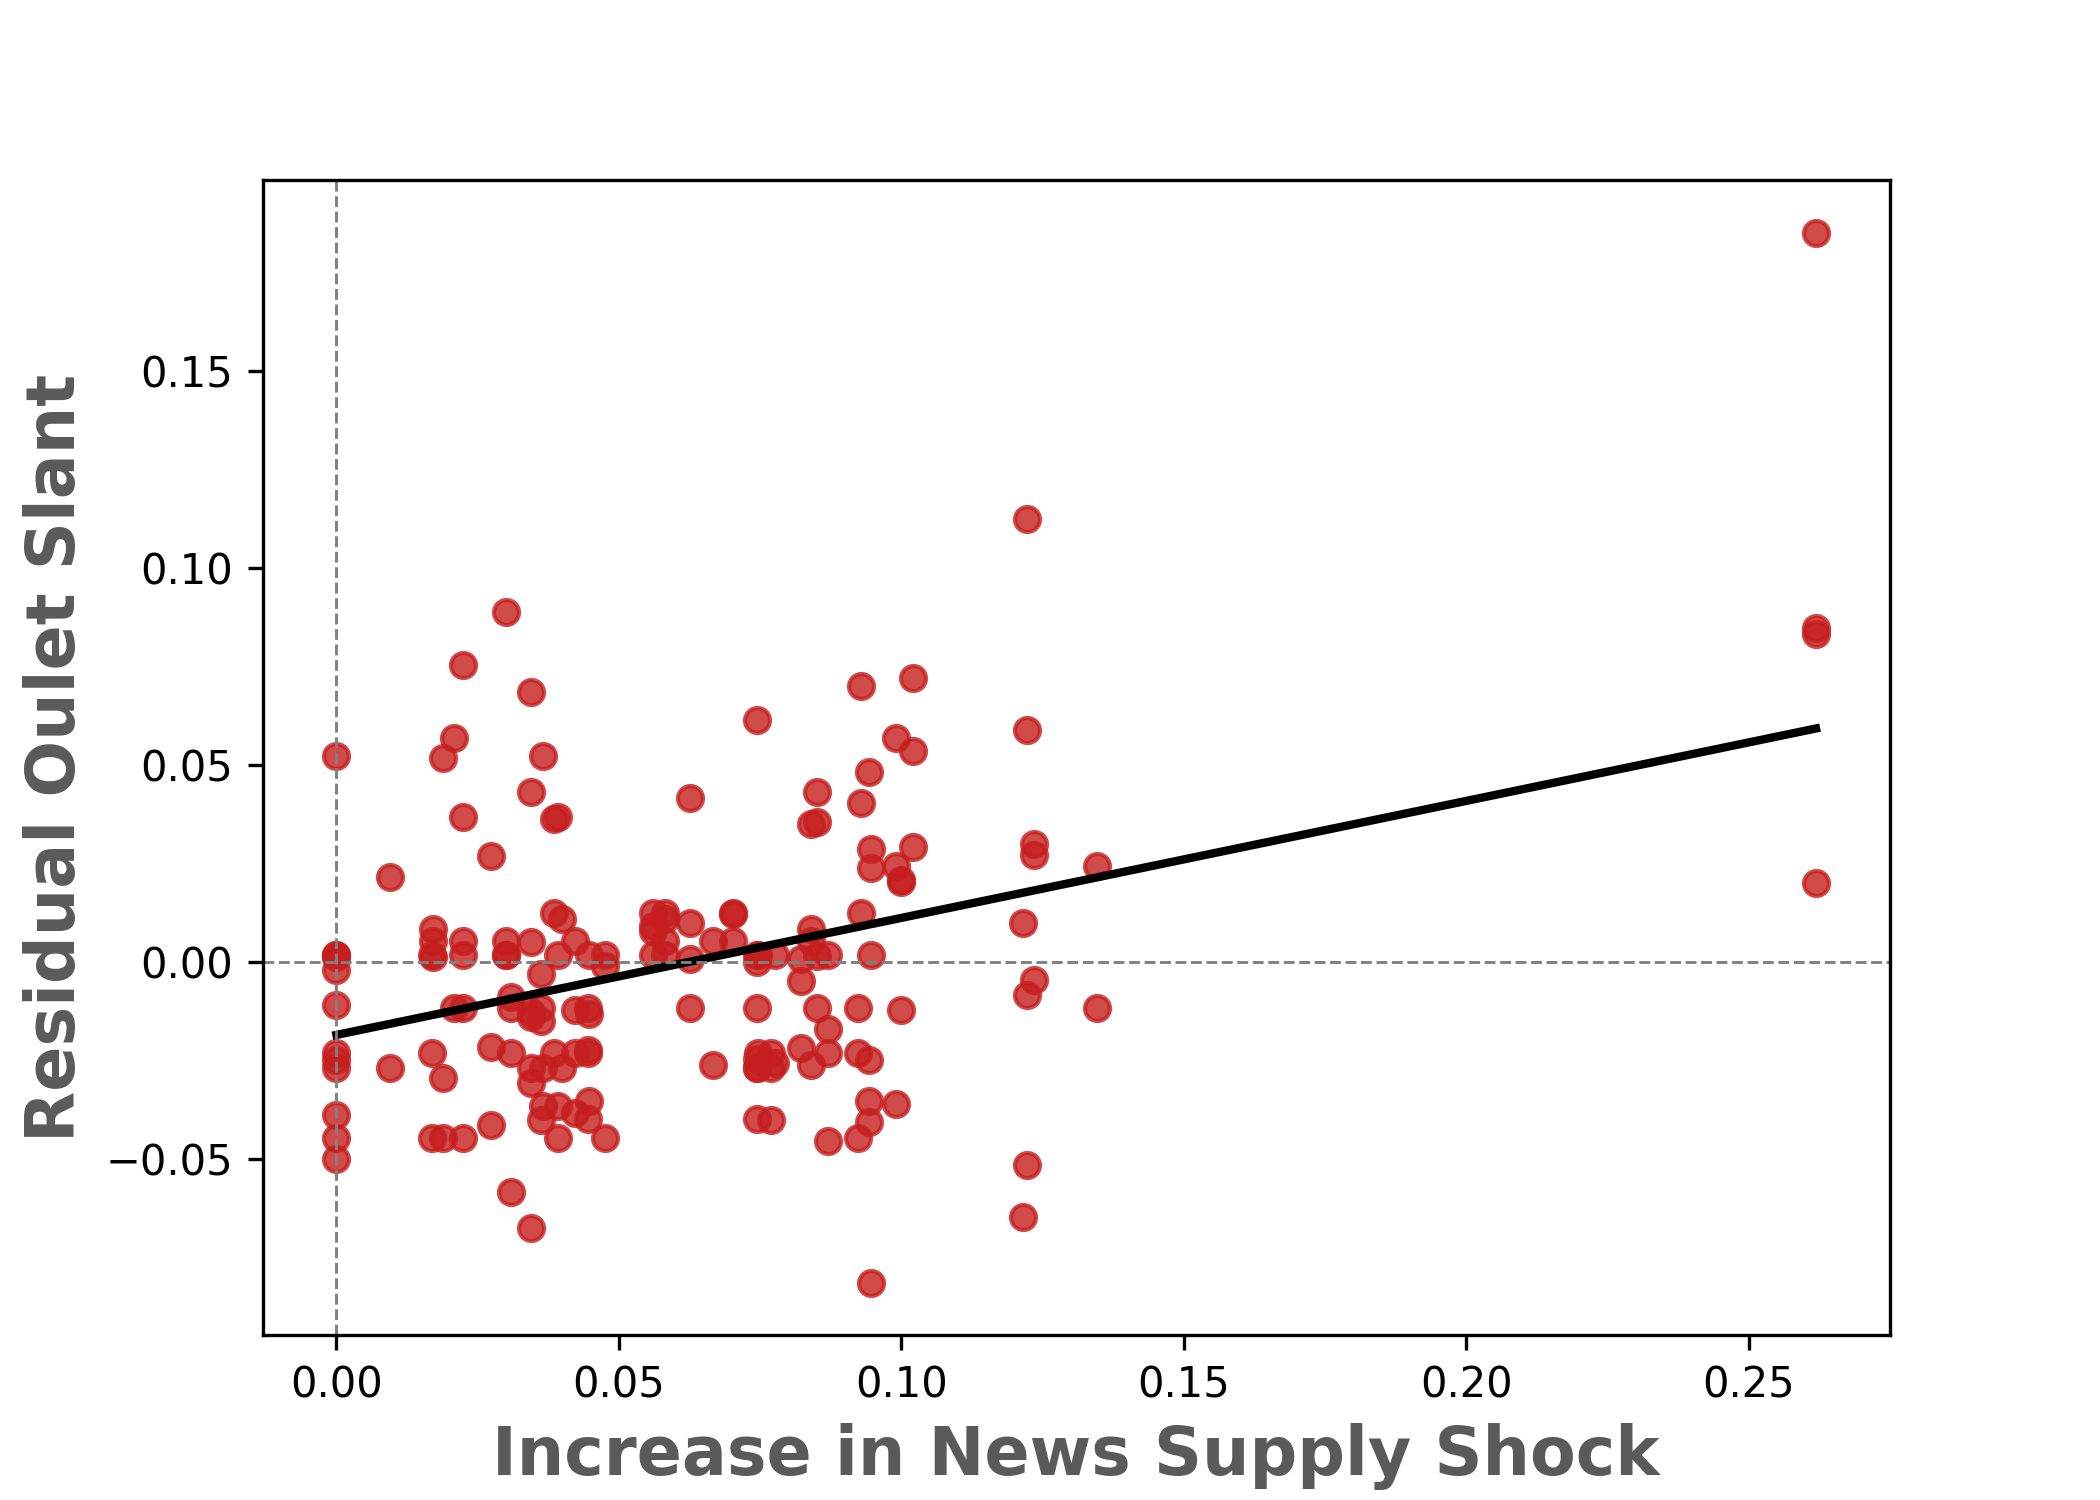
\includegraphics[width=0.45\textwidth]{figures/char_neg_left_residual_v2} &
		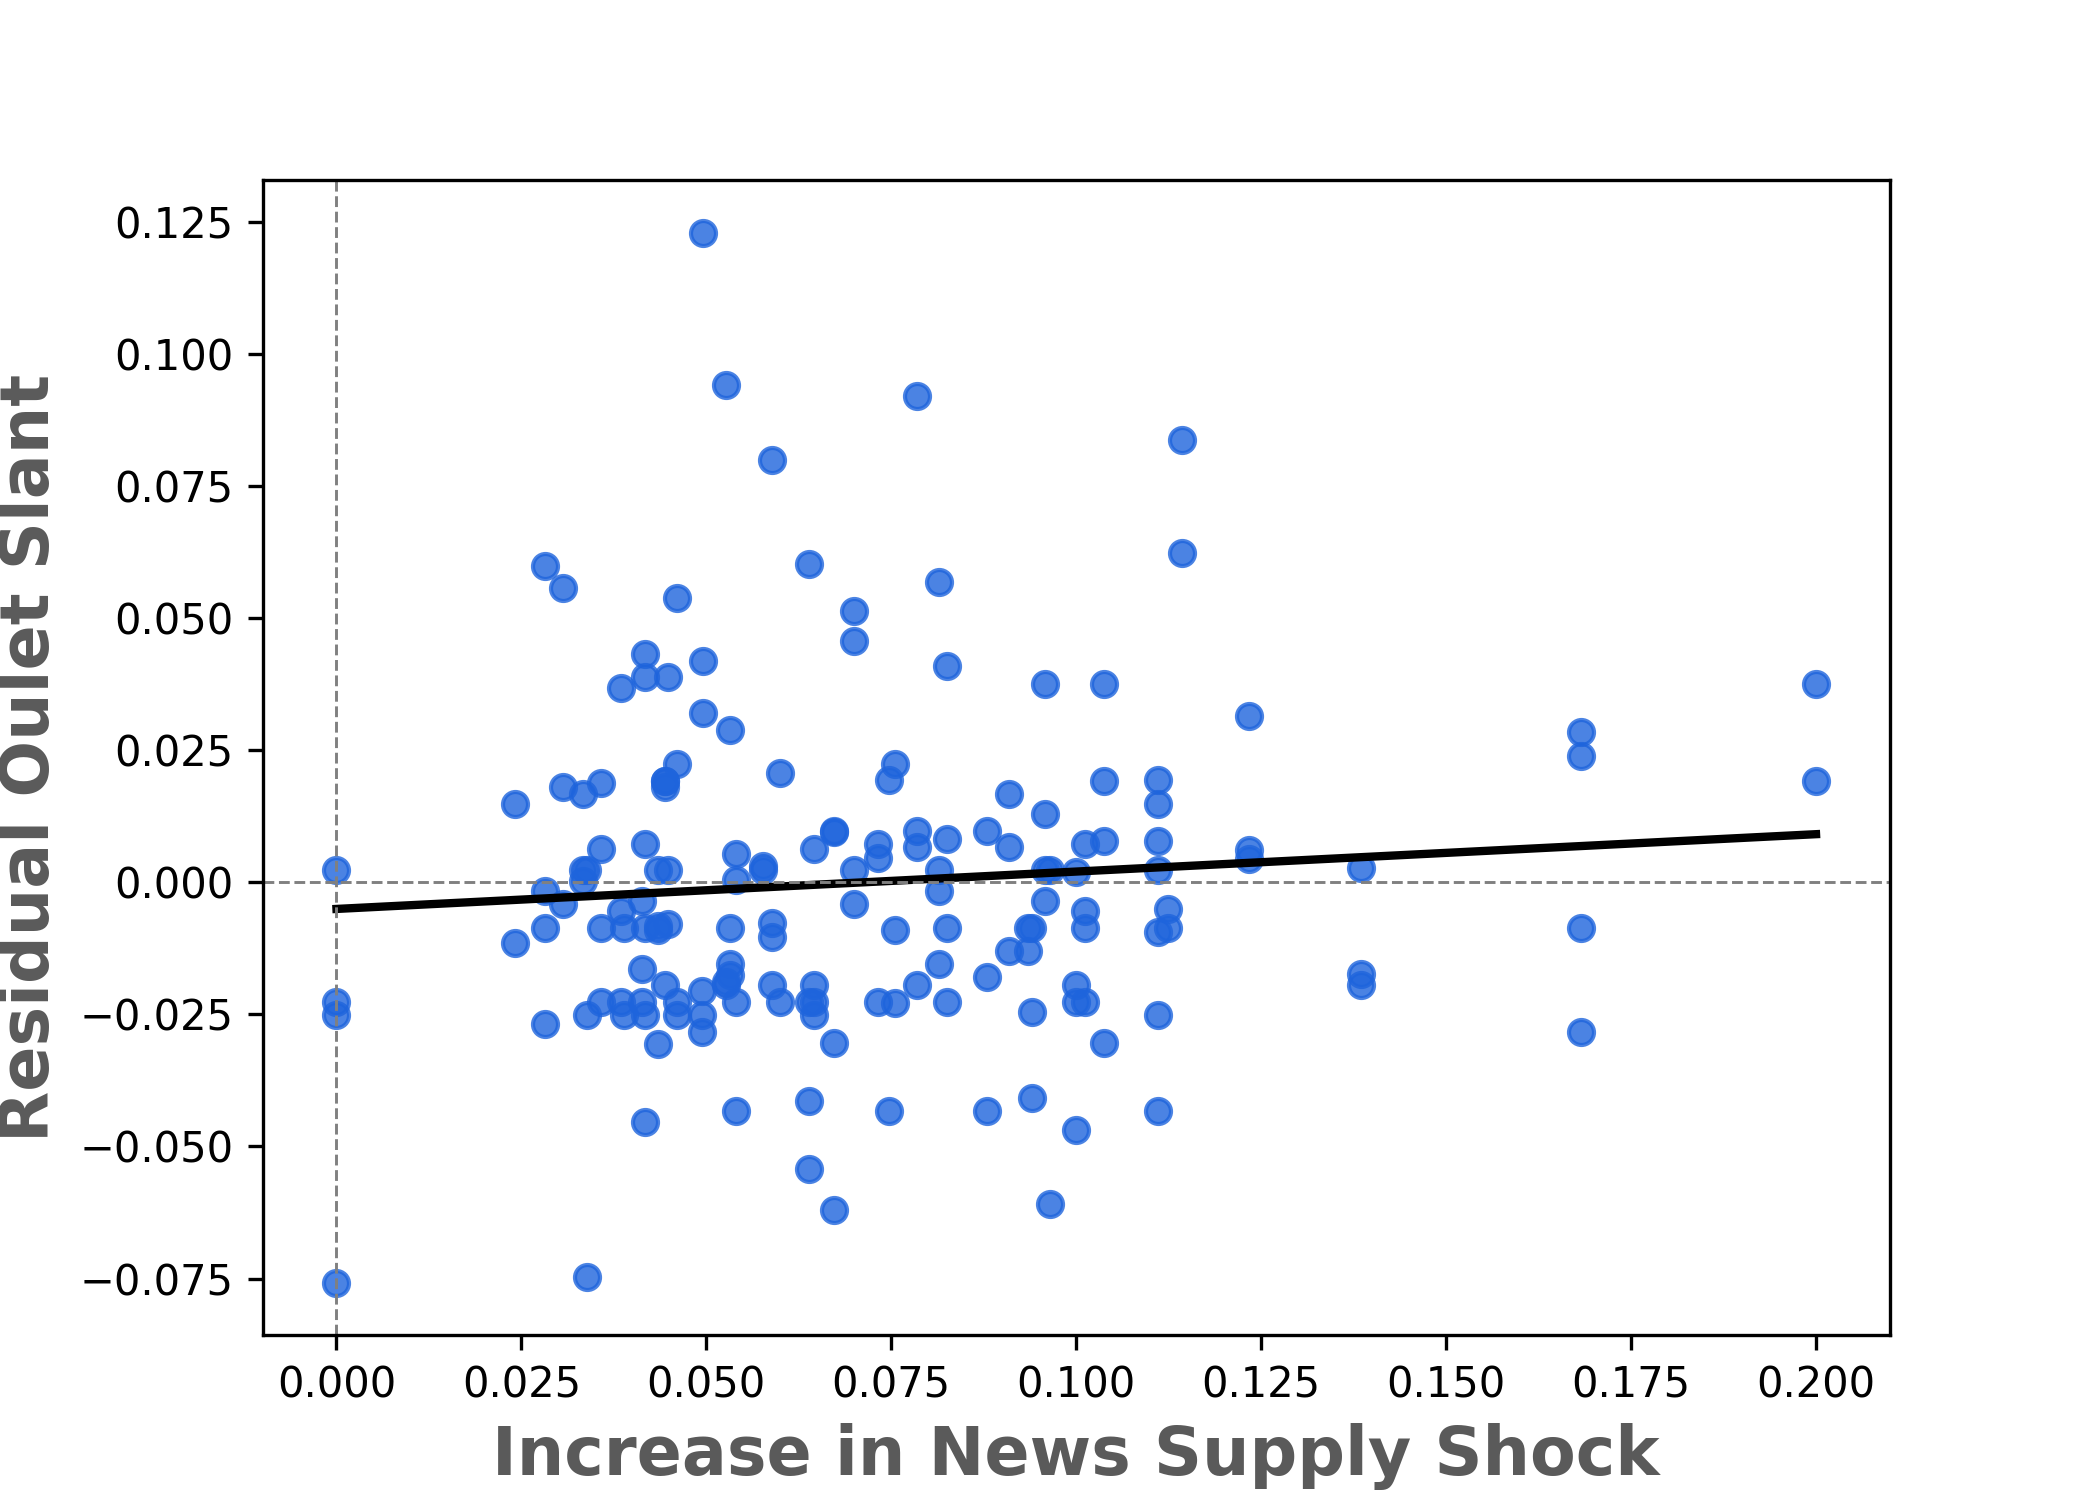
\includegraphics[width=0.45\textwidth]{figures/char_neg_right_residual_v2}
	\end{tabular}
	\caption*{\textit{Note:} Scatter with fitted line from the regression of the residual from a regression of the evening tone on the midday tone with outlet fixed effects on the tone of the stories in EFE between midday and evening.}
	\label{fig:diff}
\end{figure}



To decompose this variation by outlet, I also run regressions of the form described in  \ref{eq:first_stage} done on within day differences $ \Delta x_{jd}$ and $\Delta z_{d}$. Figure \ref{fig:fwl_diff} on the appendix shows the added variable plots. Although there is significantly less power now, the main mechanism still holds. Right (left) outlets increase more their production of stories of a given party-tone from midday to the evening editions conditional on those stories being aligned with their stances. 











Differencing~\eqref{eq:focs} eliminates the unobserved shock:
\begin{equation}\label{eq:diff_foc}
	\underbrace{%
		\sum_{r}\left(
		\frac{\partial s_{jrd+1}}{\partial x_{jd1}^k}
		-
		\frac{\partial s_{jrd+1}}{\partial x_{jd0}^k}
		\right)\frac{L_r}{L}
	}_{\Delta g_{jd+1}^k}
	\;=\;
	2\lambda_j^k
	\left(
	\frac{x_{jd1}^k-x_{jd0}^k}{\,z_{d1}^k-z_{d0}^k}
	\right)
	\;+\;
	\Delta\nu_{jd}^k \quad \forall(j,k).
\end{equation}
Intuitively, the evening–mid-day change in the gradient, $\Delta g_{jd+1}^k$, is driven by the change in story availability $(z_{d1}^k-z_{d0}^k)$, while the day-persistent cost shock cancels out. The system of equations in \ref{eq:focs} can be estimated under GMM with condition $\E \left[\left( \frac{\Delta x_{jd}^k}{\Delta z_{d}^k} \right)  \Delta\nu_{jd}^k \right]= 0 $. 



\subsection{Results of the Supply Estimation}





Table~\ref{table:costs} reports the estimated $\lambda_j^k$. \footnote{Processing of the mid‑day broadcasts for the pre‑campaign period could not be completed after the Google Cloud and OpenAI credits ended; consequently, the cost estimates here cover only the campaign window. }
Producing content favourable to the left (positive-L or negative-R)
is costlier for the right-leaning Antena~3,
while the reverse holds for left-leaning La~Sexta and TVE.  
Telecinco, a centrist outlet, faces the lowest absolute costs in every category.




\begin{table}[!htbp]
	\caption{Estimated Cost Parameters ($\lambda$) by Channel and Content Type}
	\label{table:costs}
	\centering\small
	\begin{tabular}{lcccc}
		\toprule
		& La~Sexta & TVE & Telecinco & Antena~3 \\
	& 	\scriptsize{(Left)} & \scriptsize{(Left)} & \scriptsize{(Middle)}& \scriptsize(Right) \\
		\midrule
		% Group 1
		Negative Left   
		& 12.782   &  6.614   & 108.985   & --38.135  \\
		& (44.512) & (3.107)  & (60.695)  & (24.006)  \\
				\midrule
		Positive Right  
		& --89.175 & --105.658 & --13.868  & --238.018 \\
		& (85.860) & (121.713) & (91.624)  & (77.314)  \\
		\midrule
		% Group 2
		Positive Left   
		& 36.094   &  3.368   &  25.984   & --38.962  \\
		& (52.716) & (13.110) & (43.586)  & (84.390)  \\
				\midrule
		Negative Right  
		&  4.059   & --8.694  &  30.280   &  34.624   \\
		& (4.788)  & (11.057) & (36.013)  & (53.835)  \\
		\midrule
		% Group 3
		Political 
		& --0.349  &  0.317   &   1.498   &   1.455   \\
		& (0.610)  & (0.622)  &  (1.049)  &  (1.248)  \\
		\bottomrule
	\end{tabular}
	\vspace{0.5em}
	\caption*{\scriptsize\emph{Note:} Robust standard errors in parentheses. The table shows the estimated coefficients under GMM for Equation \ref{eq:diff_foc} for the campaign period.}
\end{table}



The signs confirm the interpretation: left-favourable content is costlier for right-leaning outlets, and vice versa for all characteristics but for positive left content. It is important to remark that the interpretation of these costs parameters is broad and cannot be disentangled into different factors. Higher values of $\lambda$ could reflect costs in the production of certain content due to specialization of the journalists, having less access to information sources and/or private interests. 


Given the demand and supply estimates, in the next section I present the counterfactual analysis testing policy regulations on content. 







\FloatBarrier










\section{Proportional Air Time Rule}

\label{sec:counter}


Across Europe, broadcast regulators increasingly impose proportional-air-time rules to curb partisan imbalances in election coverage: France’s ARCOM stopwatches every political segment to enforce strict minute-for-minute equality during the “période officielle”; Italy’s Par Condicio law compels both public and private stations to “balance and compare” exposure for all lists; and Germany grants each registered party free television slots whose length scales with its prior vote share. Spain, by contrast, still relies on a voluntary pluralism. The public network TVE issues a proportional airtime manifesto while commercial groups—Atresmedia and Mediaset—entirely unconstrained. 

My model estimates allow to test what would be the implications of enforcing such policy to all the broadcasters.  I take the proportion of votes in the past general elections for each party and estimate the new equilibrium under the following problem: 



\begin{equation}\label{eq:payoffs2}
	\begin{aligned}
		\max_{\{\bm{x}_{jd}\}}   & \left\{   \sum_{r}s_{jrd+1}(\bm{x}_{jd}, \bm{x}_{-jd})\frac{L_r}{L} - \sum_k \left({\lambda_j^k}  \dfrac{(x_{jd}^k)^2}{z_{d}^k} + \eta_{jd}^k x_{jd}^k \right)  \right\}\\
		s.t.   \quad &   \frac{x_{jd}^{R+} + x_{jd}^{R-} }{x_{jd}^{political}}=vote^R\equiv0.51\\
		&  \frac{x_{jd}^{L+} + x_{jd}^{L-} }{x_{jd}^{political}}= vote^L\equiv0.49\\
       &  x_{jd}^{L+} +x_{jd}^{R+} + x_{jd}^{L-} + x_{jd}^{R-} \leq  x_{jd}^{political}\\
		& x_{jd}^k \in (0,1] \quad \forall k
	\end{aligned}
\end{equation} 


where, in a logic consistent with my measurement strategy, time to a political party can only be discerned if that story has some specific slant. I assume that the policy is enforced; that is all outlets must devote the proportion of political time given by previous proportions of votes $(vote^R, vote^L)$ (i.e constraints bind). This simplifies the choice set to $\left( x_{jd}^{L+} ,x_{jd}^{R+} ,x_{jd}^{political}\right)$. For computational constraints I i) pool left channels as a single player using thir average payoffs and ii) discretize the action space and solve for the pure Nash equilibrium after converting the game into normal form.\footnote{The code was run under a Google Cloud “n2d-standard-224” virtual machine (224 vCPUs, 896 GB RAM).}

%Another important assumption in the counterfactual analysis relates to the unobserved marginal cost shifters $\eta$ in equation \ref{eq:focs}. Since the $\lambda$ parameters were estimating by first differencing and the small sample size does not leave enough degrees of freedom to estimate $\eta_{jd}^k$ as fixed effects, these terms are not included in the cost function in the counterfactual game in \ref{eq:payoffs2} (i.e I assume $\bm{\eta}= \bm{0}$).



I recover an estimate of $\eta_{jd}^k$ from the level first-order condition in \eqref{eq:focs}. Define the residual
\[
r_{jdh}^k \;\equiv\; g_{jdh+1}^k \;-\; 2\,\hat\lambda_j^k\,\frac{x_{jdh}^k}{z_{dh}^k}
\;=\; \eta_{jd}^k + \nu_{jdh}^k ,
\]
and estimate the day shock by the edition-average residual
$\hat\eta_{jd}^k \equiv \tfrac{1}{2}\big(r_{jd0}^k+r_{jd1}^k\big)$, which is unbiased under zero-mean edition noise. In the counterfactual problem \eqref{eq:payoffs2} I treat $\hat\eta_{jd}^k$ as given (fixed by day and channel) and solve for best responses under the policy constraints, so changes arise from the policy, not from altering day-specific costs.


Results of the counterfactual estimation are shown in Table \ref{tab:counter}.  The left columns report the factual, average minutes for each category during the campaign and the right column the results from the counterfactual estimation. 



\begin{table}[!htbp]
	\caption{Factual and Counterfactual Slant by Channel}
	\label{tab:counter}
	\centering\small
	\begin{tabular}{lcccccc}
		\toprule
		& \multicolumn{2}{c}{La~Sexta/TVE} & \multicolumn{2}{c}{Telecinco} & \multicolumn{2}{c}{Antena~3} \\
		& \multicolumn{2}{c}{(Left)} & \multicolumn{2}{c}{(Middle)} & \multicolumn{2}{c}{(Right)} \\
		& Factual & Count. & Factual & Count. & Factual & Count. \\
		\midrule
		Negative Left & 0.06 & 0.05 & 0.04 & 0.36 & 0.09 & 0.45 \\
		\midrule
		Positive Right & 0.03 & 0.00 & 0.03 & 0.00 & 0.04 & 0.01 \\
		\midrule
		Positive Left & 0.09 & 0.10 & 0.04 & 0.10 & 0.06 & 0.01 \\
		\midrule
		Negative Right & 0.09 & 0.15 & 0.04 & 0.44 & 0.07 & 0.43 \\
		\midrule
		Political & 0.42 & 0.30 & 0.18 & 0.90 & 0.39 & 0.90 \\
		\midrule
		\bottomrule
	\end{tabular}
	\vspace{0.5em}
	\caption*{\scriptsize\emph{Note:} Table shows the average proportion of minutes from the counterfactual Problem \ref{eq:payoffs2} for the campaign period.  Parenthesis show the deviation across dates. I consider only dates with a unique, pure Nash equilibrium.}
\end{table}


Several facts emerge from the counterfactual exercise. First, left-leaning outlets (La Sexta/TVE) reduce the overall share of political coverage from 42\% to 30\% when constrained to allocate airtime proportionally. Since they are forced to spend more time on right wing coverage, they cut back on politics altogether and shift tone toward more negative tone of the right (from 0.09 to 0.15). At the same time, their positive coverage of the left remains broadly unchanged, implying that compliance is achieved primarily by eliminating right-positive content and compensating with hostile tone.


Second, the centrist outlet (Telecinco) responds by dramatically expanding its political content, from 18\% of airtime in the factual data to 90\% in the counterfactual. This increase comes almost entirely in the form of negative tone: coverage harming the right grows more than tenfold (from 0.04 to 0.44), and coverage harming the left rises sharply as well (from 0.04 to 0.36). In other words, proportional airtime regulation induces Telecinco to turn heavily partisan, despite its relatively neutral baseline position.

Third, the right-leaning outlet (Antena 3) also amplifies its use of negative tone. Its political coverage rises from 39\% to 90\%, with negative coverage of both left and right parties soaring (0.09 to 0.45 and 0.07 to 0.43, respectively). Positive coverage, by contrast, collapses to near zero.


Taken together, these adjustments generate a markedly more polarized landscape. Figure \ref{fig:change_line_counter} illustrates the resulting shifts in outlets’ ideological positions: left-leaning and centrist outlets move further left, while Antena 3 strengthens its rightward tilt. Importantly, the regulation compresses the space for balanced coverage by forcing all outlets to increase political airtime but leaving tone unconstrained. Dispersion across channels increased from 0.06 to 0.20 with a notable increase in the standard deviation from 0.03 to 0.1; leading to a highly more polarized media environment. 





	
	\section{Conclusion}
	\label{sec:conclusion}
	
\begin{comment}
	content...

	
	XXX
	
	
1) This paper studies how campaigns affect demand for political content. 

2) i predent a strucutral model that covers both the demand and supply of news

3) fit the model to spain + data used. 

4) demand: BLP model + identification + results (affectivepolarization + ER)

5) Supply: identification + results

6) counterfactuals

7) Overall this paper. Long run effects of polarization, importance of traidional media, drawbacks with i) measurement and ii) regulations.
	
XXX

\end{comment}

This paper studies how election campaigns affect the demand for political content. I develop a structural model that incorporates both the demand and supply sides of television news, in which viewers choose among outlets while broadcasters strategically set the partisan tone of their political coverage.
	
	
	
	
	I apply this framework to Spain during the 2023 general election, assembling a novel dataset that combines self-collected transcripts of prime-time broadcasts with minute-level audience-meter data. On the demand side, I estimate a BLP-style random-coefficients model, identified through exogenous variation in the daily newswire mix. The results indicate that affective polarization in news consumption appears only during the campaign period: in right-leaning regions, an additional minute of positive coverage of right parties is associated with roughly 3{,}000 extra viewers relative to off-campaign, while more negative-right tone corresponds to losses on the order of 8{,}000 viewers, with mirrored patterns in left-leaning regions. Furthermore, polarization in media consumption lines up with political polarization: those regions with more polarized news demand also register higher political polarization. The campaign constituted a structural break in political polarization. The gap comes from regions that present high polarzation in their media consumption and remains increaing for more than one year after the break. 
	

	
	Given the estimated demand parameters,  I recover broadcasters’ cost structures by exploiting within-day variation in the availability of partisan stories between midday and evening editions. The estimates point to asymmetric costs consistent with editorial orientation—pro-left content proves costlier for right-leaning outlets, while the reverse holds for left-leaning outlets, and centrist channels face the lowest absolute costs.
	
Building on these demand and supply estimates, I evaluate counterfactual scenarios where proportional airtime regulations are enforced. The simulations indicate that while such rules succeed in balancing exposure time across parties, they inadvertently amplify polarization by encouraging outlets to shift along the tone dimension. In equilibrium, this substitution results in sharper partisan contrasts and more polarized content than under the status quo.

Taken together, the results show that polarization in news consumption intensifies around campaigns and leaves persistent traces beyond the election period, underscoring the central role of traditional broadcast media in shaping political information. At the same time, the analysis highlights two challenges for scholars and policymakers: measurement, as slant and ideology are difficult to observe precisely and aggregate audience data blur selection from persuasion effects; and regulation, as rules focused narrowly on airtime may backfire if they neglect the tone of coverage. The structural model presented here provides a framework to evaluate such policies in equilibrium and to design interventions that jointly consider both the quantity and sentiment of political coverage.
	

	
	
	%\nocite{*}
	\clearpage
	%\addcontentsline{toc}{chapter}{Bibliography}
	%\printbibliography
	
	%\addcontentsline{toc}{chapter}{Bibliography}
	\pagestyle{plain}  
	\bibliographystyle{apa}
	
	\bibliography{./bib/media_bias.bib}
	
	
	
	\clearpage

\appendix

\addcontentsline{toc}{section}{Appendix} % Add the appendix text to the document TOC
\part{Appendix} % Start the appendix part

\parttoc % Insert the appendix TOC


\renewcommand\thefigure{\thesection.\arabic{figure}}   
\renewcommand\thetable{\thesection.\arabic{table}}
\setcounter{table}{0}


\clearpage






\section{Data Pipeline  Details}\label{sec:appendix_models}



This appendix describes the end-to-end pipeline used to collect, process, and analyze Spanish prime-time newscasts. The workflow follows Appendix Figure~\ref{fig:pipeline}: daily recordings are stored, audio is extracted and transcribed, text is segmented into minute-level stories, topics are estimated with a topic model, and political tone is classified with a large language model. The corpus comprises the midday and evening national newscasts of TVE, Antena~3, La~Sexta, and Telecinco, totaling {563 hours} of programming stored and versioned in Google Cloud Storage (GCS) \footnote{This project has been supported by Google Cloud for Education credits and OpenAI research credits.} %with a total value spent of 5,747 and 2,245 euros, respectively. }






\begin{figure}[!htb]
	\centering
	\caption{Pipeline for Content Downloading and Classification }
	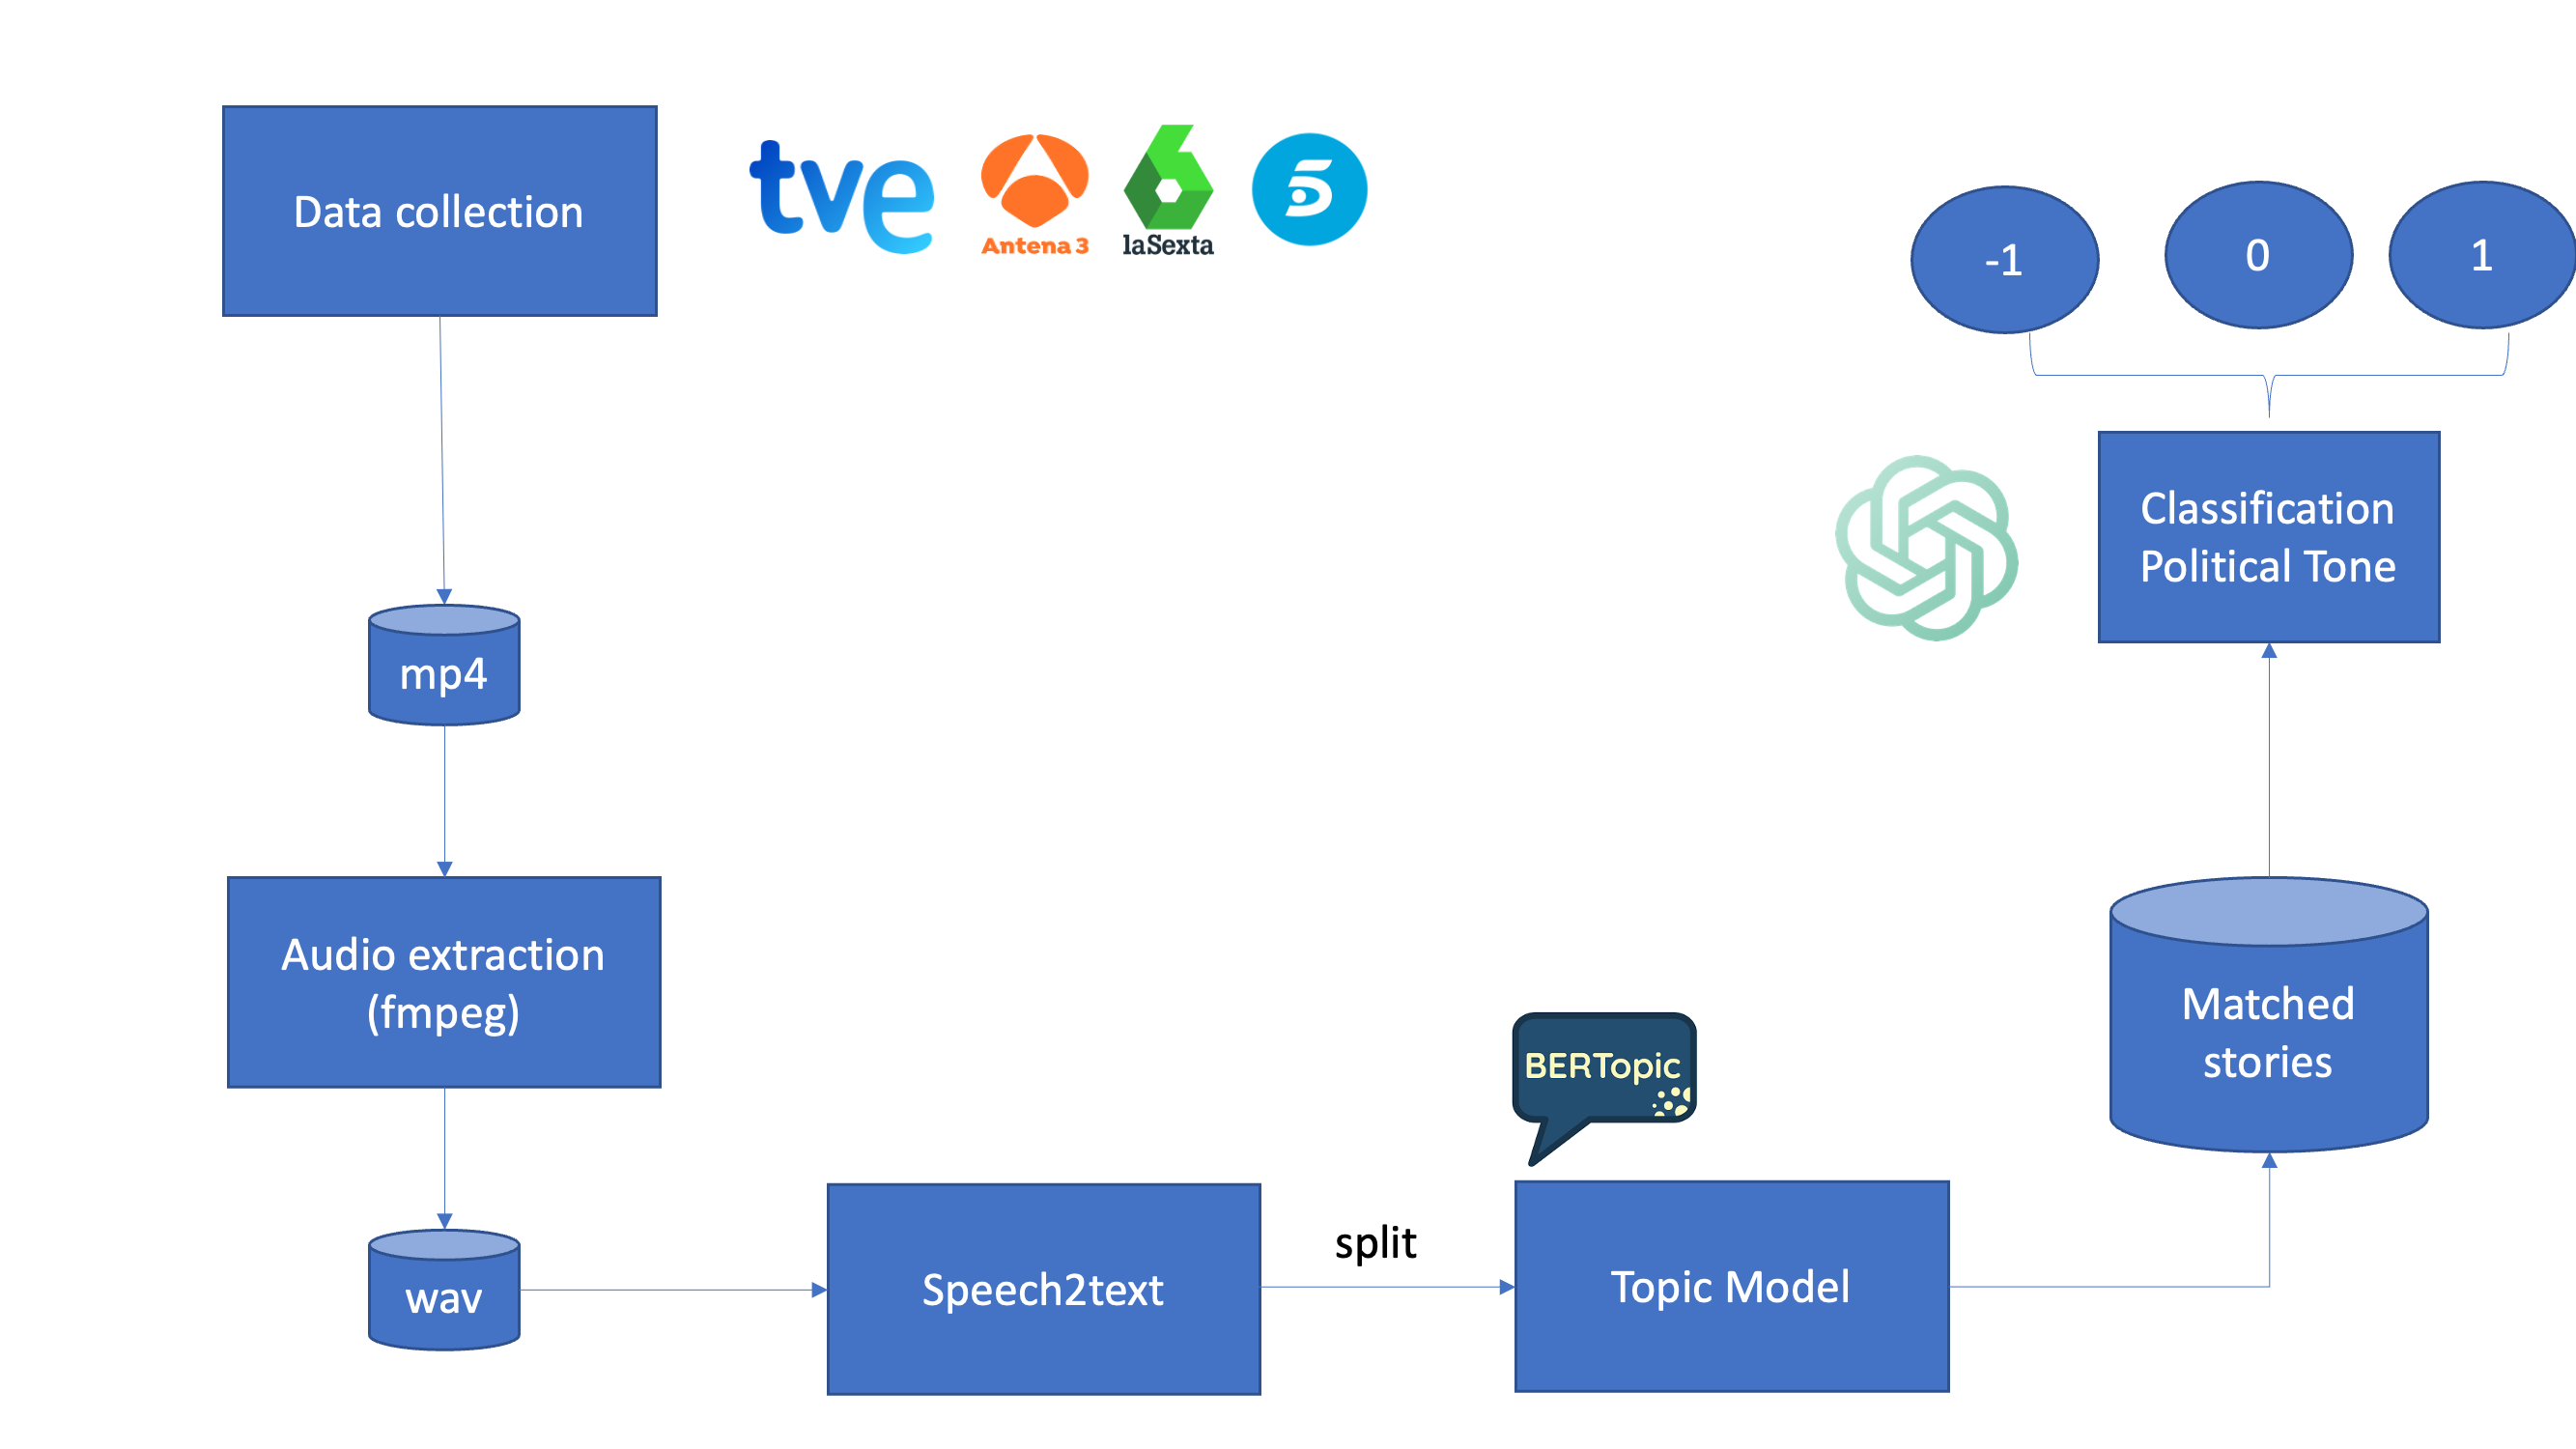
\includegraphics[width=150mm]{figures/pipeline3}
	\caption*{\small \textit{Note:} Pipeline for the text downloading. First videos are downloaded daily from the main TV channels. Google engine is used to convert the audio to text. I then split the stories by minute and use BERTopic to classify and match them. Finally, ChatGPT4 is used to classify political tone.}
	\label{fig:pipeline}
\end{figure}



\textbf{Audio and transcription.} Each broadcast is converted from MP4 to mono PCM WAV to standardize the input for automatic speech recognition. Transcripts are obtained with \emph{Google Cloud Speech-to-Text} (language \texttt{es-ES}, long-running recognition with automatic punctuation). The service returns time-stamped transcripts; for each show I archive the raw JSON and a lightly normalized plaintext transcript.

\textbf{Segmentation and alignment.} Newscasts are split into minute-level stories using program timestamps and textual cues (anchor transitions and title cards). 

\textbf{Topic discovery.} Topics are estimated with \emph{BERTopic} using multilingual sentence embeddings (\texttt{paraphrase-multilingual-MiniLM-L12-v2}). After fitting, outlier reduction and topic updates are applied; residual or incoherent clusters are flagged and excluded from matched comparisons.

\textbf{ChatGPT ideology classification.} Story-level political tone is obtained with ChatGPT on a discrete grid per party. To reduce computational and monetary costs, I first filter the set of minute-level stories using a dictionary of political keywords (Table~\ref{table:politics}); the final classification set contains 15{,}406 stories. The prompt used in the classifier is:

\begin{tcolorbox}[colback=blue!5!white, colframe=blue!75!black, title=Prompt]
	Analyze the sentiment of the following news article with respect to the political parties (and their members) in Spain: PP, Podemos/Sumar, PSOE, VOX. Only use numeric values from the set [-1, -0.5, 0, 0.5, 1].
	
	Evaluate the sentiment towards each party with a number between -1 and 1, where -1 indicates an extremely negative perception, 0 indicates neutrality or irrelevance for the party, and 1 indicates an extremely positive perception.
	
	Consider only the values -1, -0.5, 0, 0.5, and 1.
	
	Base your evaluation solely on the explicit content of the news article. If the article does not mention or imply any sentiment towards a party, assign a 0 to that party.
	
	The format must always be a list \texttt{[PP
		, PSOE
		, UP
		, VOX
		]} where \texttt{X} represents the numeric sentiment value.
\end{tcolorbox}

\noindent\textit{Note:} Prompt used under \textit{gpt-4-0125-preview}. Story-level tones are aggregated to the program–day level with duration weights (seconds per story). Channel-level summaries are constructed by averaging across program–days, and matched-story comparisons are restricted to aligned topic–day pairs.



\newpage




\section{Robustness of the Text Classification}

\label{sec:robustness}







\subsection{Comparison with Previous Approaches}


One concern with LLMs classification is whether they can consistently capture meaningful patterns in text to distinguish tone. Table \ref{tab:top_trigrams} shows the most frequent three-word sequences across each sentiment–ideology category. The trigrams in the “Positive Right” column center on leadership titles and formal roles, reflecting an organizational focus; those in “Negative Right” cluster around legal and procedural language, indicating contexts of investigation or trial. The “Positive Left” trigrams emphasize policy areas and sectoral initiatives, suggesting substantive, topic-driven framing, while the “Negative Left” sequences feature judicial and procedural terms, pointing to oversight and legal scrutiny. Specific examples of stories can be seen in Appendix Table \ref{tab:examples_stories}.


To assess robustness, I also compare the LLM’s classifications with those obtained using methods from previous works \citep{gentzkow2010media,laver2003extracting}. I use all Spanish congress speeches during my sample period and exploit party labels to assess similarities with the outlets’ content. 


Similar to \cite{gentzkow2010media} and \cite{laver2003extracting} I exploit party ideology in congress speeches to calculate similarity measures of the outlet's speech. I make use of all congressional speeches produced during my sample period and associate each speaker with their respective political party, filtering to retain the set of relevant parties.

I follow a similar, non-linear version of \cite{laver2003extracting} and create a score for each word $w$ in the congress speech as: 



\begin{equation}
	\text{Score}(w) \;=\; \ln \left( \frac{\mathrm{freq}(w,\text{Left}) + \alpha}{\mathrm{Total}_{\text{Left}} + \alpha} \right) \;-\; \ln \left( \frac{\mathrm{freq}(w,\text{Right}) + \alpha}{\mathrm{Total}_{\text{Right}} + \alpha} \right),
	\label{eq:log_ratio}
\end{equation}

where:
\begin{itemize}
	\item $\mathrm{freq}(w,\text{Left})$ is the number of times word $w$ appears in the speeches of left-leaning parties (PSOE and UP),
	\item $\mathrm{Total}_{\text{Left}}$ is the total word count in left-party speeches,
	\item $\mathrm{freq}(w,\text{Right})$ and $\mathrm{Total}_{\text{Right}}$ are defined analogously for right-leaning parties (PP and Vox), and
	\item $\alpha$ is a small smoothing parameter.
	
\end{itemize}

I select the value of alpha that maximizes accuracy of label prediction in the congress dataset; $\alpha=0.9$.	
Words with high positive scores are used disproportionately in left-leaning speeches, while those with high negative scores are more characteristic of right-leaning speeches. I rank all words by their computed score and select the top 100 left-coded words and top 100 right-coded words, represented in  Figure  \ref{fig:wordcloud}. 






\begin{figure}[htbp!]
	\caption{Word Cloud Congress Speeches}
	
	\centering
	%— Left pane —
	\begin{minipage}{0.46\textwidth}
		\centering
		\textbf{(a) Top Left Words}\\[1ex]
		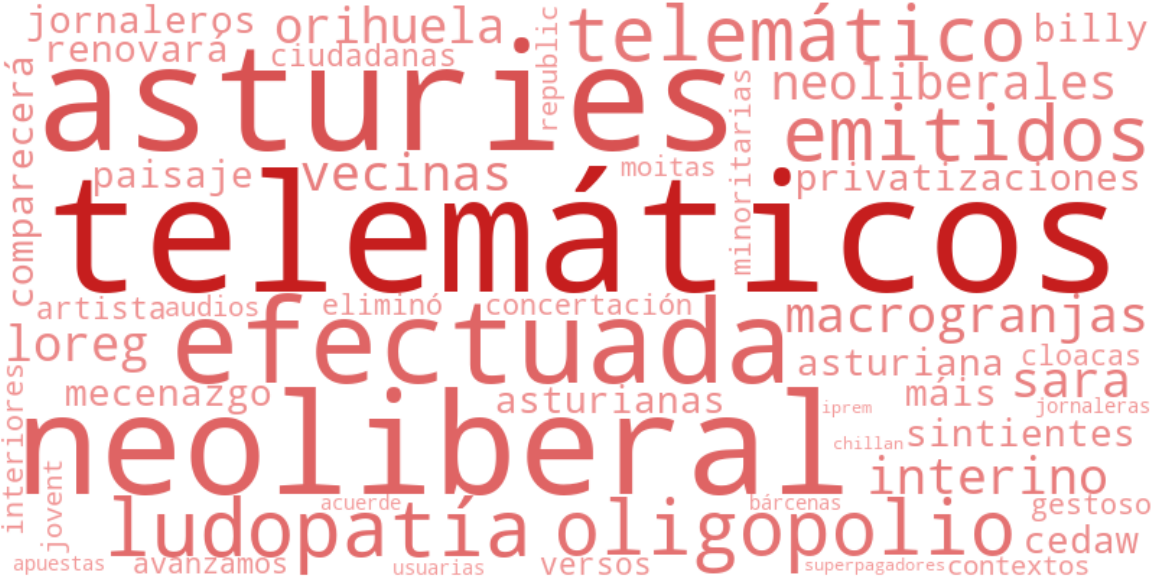
\includegraphics[width=\linewidth]{figures/congress_left.pdf}
	\end{minipage}%
	\hfill
	%— Right pane —
	\begin{minipage}{0.46\textwidth}
		\centering
		\textbf{(b) Top Right Words}\\[1ex]
		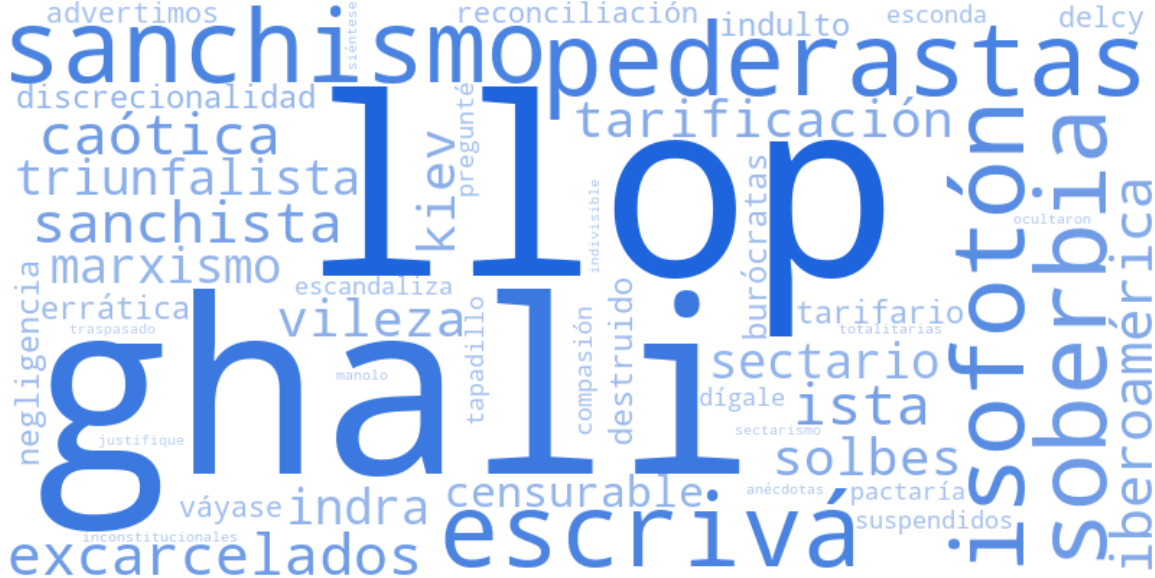
\includegraphics[width=\linewidth]{figures/congress_right.pdf}
	\end{minipage}
	
	%— Shared caption and note —
	
	
	\vspace{0.5ex}
	
	{\small
		\textit{Note:} The wordclouds represent the top words with lowest (left) and highest (right) scores as defined in equation~\ref{eq:log_ratio}. Size is weighted by word-frequency.
	}
	\label{fig:wordcloud}	
\end{figure}



The word clouds make clear the distinctive use of language by parties in congress. On the left, for example, the large term “neoliberal” (neoliberalism) underscores an ongoing critique of market‐driven reforms, while “oligopolio” (oligopoly) highlights concerns about concentrated economic power. On the right, “sanchismo” (literally “Sánchez-ism”) signals frequent reference to the governing style of Prime Minister Sánchez as a political brand, and “pederastas” (pederasts) reveals the use of morally charged scandal language with the ley solo sí es si scandal. 





Figure \ref{fig:congress_line} shows the left–right positions derived from this method. Although the overall ranking of the outlets from left to right is consistent with the ChatGPT classification in Figure \ref{fig:chat}, the middle channel is now classified as left-wing, close to the public channel. 


\begin{comment}
	content...

\begin{figure}[htbp!]
	\centering
	\caption{Normalized Ideology Scores from Congress Speeches}
	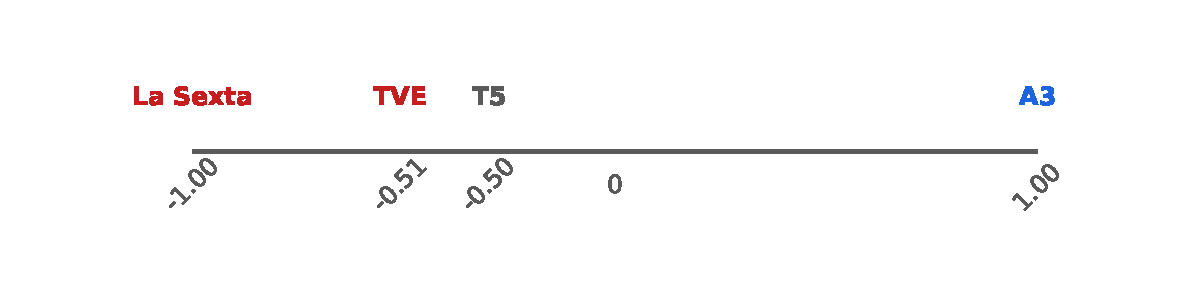
\includegraphics[width=120mm]{figures/congress_line}
	\caption*{\small  \textit{Note:} The figure shows the normalized ideology positions of the channels after the text classification based on congress speeches as described by Equation \ref{eq:log_ratio}}

\end{figure}
\end{comment}






	\begin{figure}[!htbp]
	\centering
	\caption{Normalized Ideology Index by Channel}
	
	% Panel (a): ChatGPT-based
	\begin{minipage}[t]{0.49\textwidth}
		\centering
		(a) Demand: Viewers' ideology
		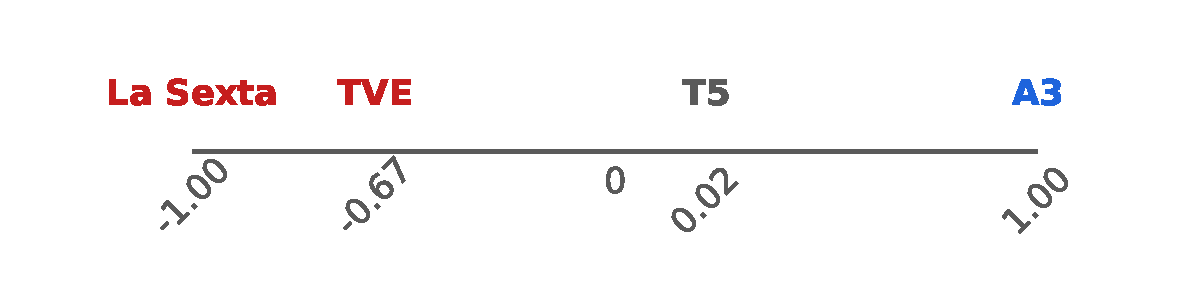
\includegraphics[width=\linewidth]{figures/congress_line_cis}
	\end{minipage}
	\hfill
	% Panel (b): CIS-based
	\begin{minipage}[t]{0.49\textwidth}
		\centering
		
		
		(b) Supply: Text classification 
		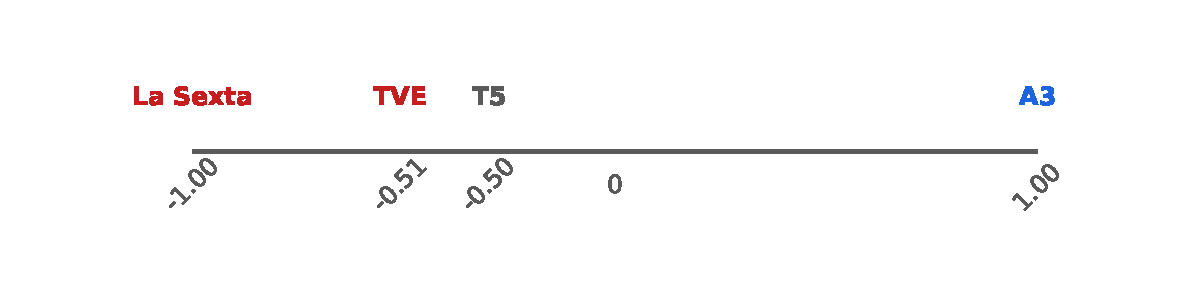
\includegraphics[width=\linewidth]{figures/congress_line}
		

	\end{minipage}
	
	
	\caption*{\small \textit{Note:} The figure compares normalized left–right positions for the outlets in the sample. Panel (a) uses viewer ideology data from CIS survey data, using the difference in correlation coefficients between right and left; panel (b) uses ChatGPT-based text classification net tone as described in Equation \ref{eq:log_ratio}. Values are normalized so that the two most extreme channels take values -1 and 1. }
	\label{fig:congress_line}
\end{figure}




Two remarks are worth mentioning. First, it is important to note that this comparison against survey data might entail some issues. Declared preferences can serve as validation under the assumption of channels' decisions being heavily driven by demand preferences rather than other factors. Cross-validation of human annotators on the labels of political stories would be an alternative way to check out the results. 

Second, reducing each story to a single left–right score aids interpretation, but ignores the multidimensional nature of politics highlighted by \citet{puglisi2011newspapers}. Economic versus cultural cleavages, or regional versus national frames, may evolve differently and deserve separate tracking. I leave extending the LLM classifier to a low-dimensional vector of ideological dimensions for future work.




\subsection{Stability of the Classifier}


Due to their inherent stochasticity, repeated queries using the same prompt may yield different classifications \citep{llmstability2024}. As shown in \citep{llmclassification2024}, this variability can introduce noise in tasks that require high consistency, particularly in content classification. To mitigate this issue, I leverage OpenAI’s “functions” tool, which constrains the classifier’s responses to predefined discrete numerical outputs, reducing potential inconsistencies. Table \ref{tab:table_stability} presents the mean classification scores from 100 iterations of a random sample of political stories \footnote{Good practices recommend to run the classification multiple times and average out the results \citep{tornberg2023}. Financial costs, however, impede me from doing the whole approach multiple times}, along with the corresponding standard errors. The relatively small standard errors suggest that, despite the model’s stochastic nature, the classification remains stable.





\begin{table}[!htb]
	\centering
	\caption{Mean and Standard Error for 100 Rounds of ChatGPT Classification}
	\begin{tabular}{|l|c|c|c|c|}
		\hline
		\textbf{Statistic} & \textbf{PP} & \textbf{PSOE} & \textbf{VOX} & \textbf{UP} \\
		\hline
		Mean & -0.014 & 0.106 & -0.053 & 0.024 \\
		Standard Error & 0.003 & 0.004 & 0.001 & 0.002 \\
		\hline
	\end{tabular}
	\caption*{Note: The table shows the mean and standard error for 100 rounds of ChatGPT classification of political content with 40 random political stories.}
	\label{tab:table_stability}
\end{table}









\subsection{Text vs.\ Image}




Imagery is a key component of television. This may be especially relevant for political actors, for whom televised coverage has been shown to magnify the impact of candidates’ physical appearance on voter perceptions and electoral outcomes \citep{Lenz2011LookingTP}. Imagery in the form of time devoted to candidates further constitutes the main metric used by regulatory agencies. For example, the French media authority ARCOM publishes monthly “pluralism” reports that track each political actor’s share of speaking time on national television; Italy’s Osservatorio di Pavia produces similar statistics for the national regulator AGCOM. These metrics have also been used extensively in research as measures of slant \citep[see, e.g.,][]{CageHengelHerveUrvoy2022,durante2012partisan}.

Here I compare some of these approaches to my text-based measure. Due to computational constraints, I cannot perform image detection across my full video sample. Instead, I compare image-based and text-based metrics using a random sample of 67 days. Specifically, I train a state-of-the-art face recognition system \citep{face_recognition} using labeled images of the main party leaders: Pedro Sánchez (PSOE), Alberto Núñez Feijóo (PP), Santiago Abascal (VOX), and Yolanda Díaz (UP). I then extract frames from the first 25 minutes of each prime-time news broadcast across major channels, resulting in a sample of 79,788 images. Using the \texttt{face\_recognition} library, I detect and identify faces in each frame. This allows me to construct a frame-level dataset of visual exposure, which I aggregate at the daily level for each channel and party leader.

The net tone on the sample of days for each channel and political leader is shown in Figure 	\ref{fig:tone_channel}. As expected, significant differences appear, positioning channels in the left-right spectrum shown before. 


\begin{figure}[htbp!]
	\caption{Net Tone per Channel and Politician}
	\centering
	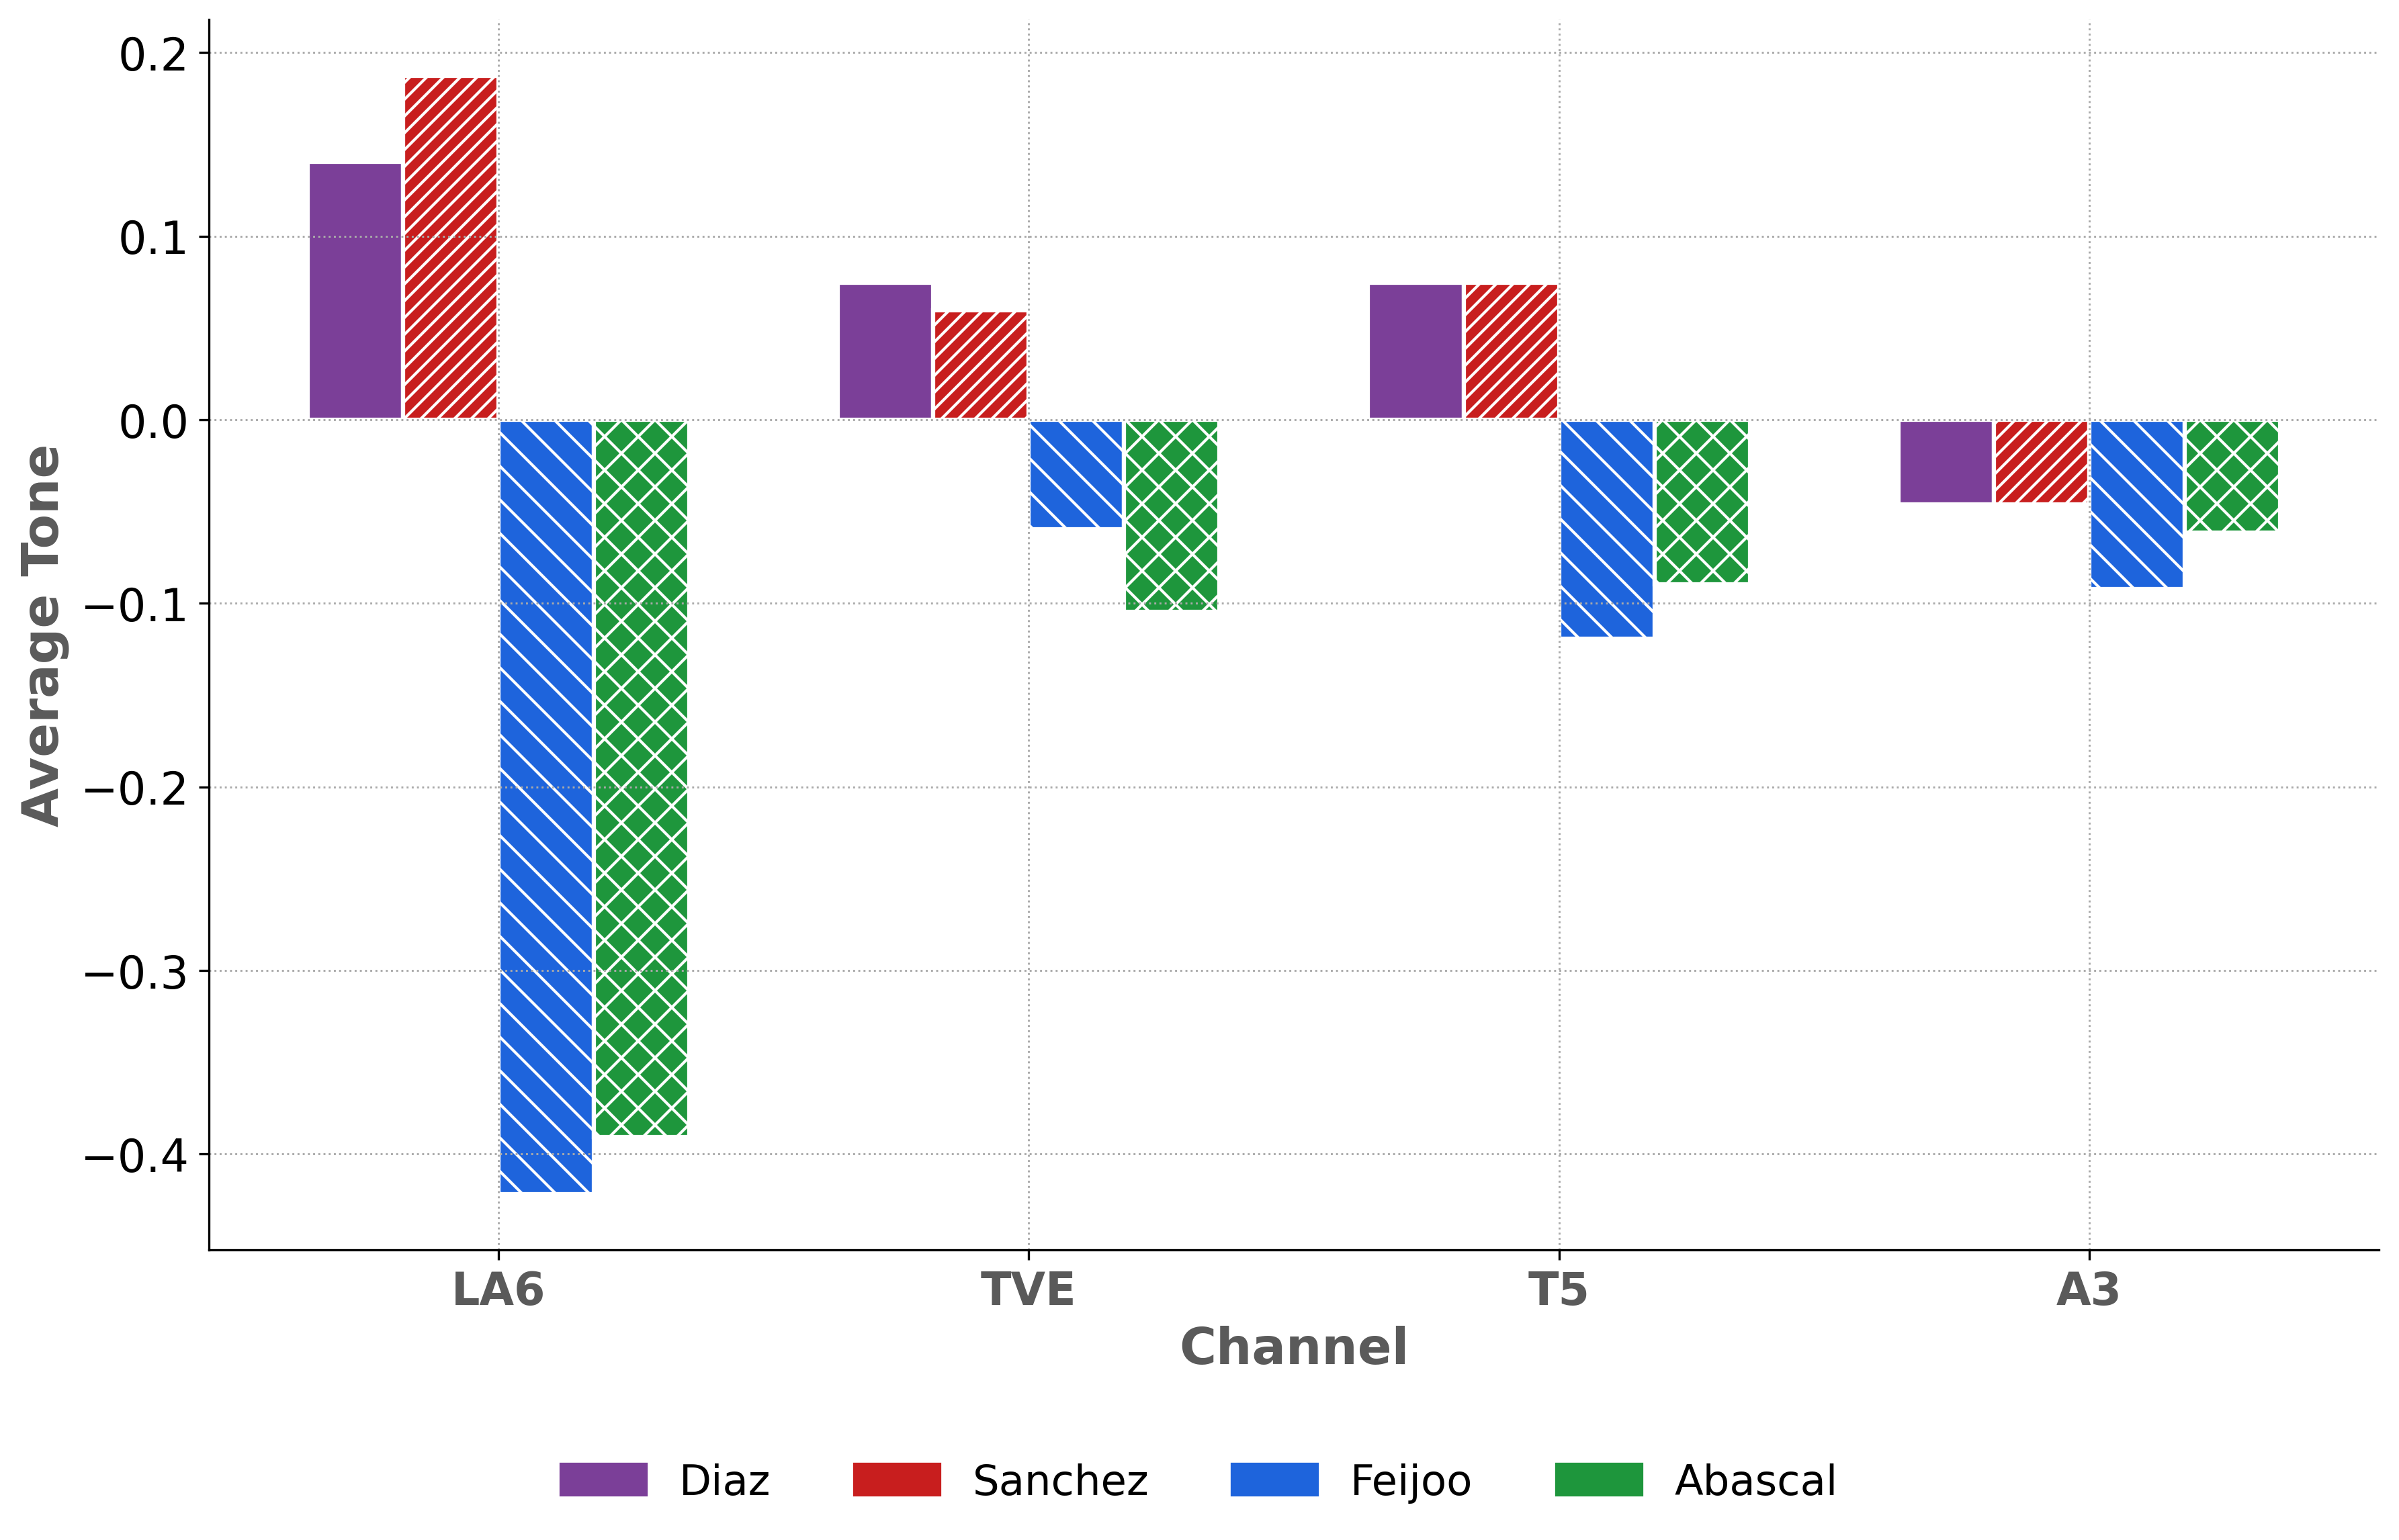
\includegraphics[width=150mm]{figures/politicians_tone_proportions}
	\caption*{\small \textit{Note:} The figure shows the net tone based on the ChatGPT classification by political actor and channel for a random sample of 67 days. }
	\label{fig:tone_channel}
\end{figure}





Next, I compare if visuals or tone follow a similar scenario. Figure \ref{fig:combined_channel} panel a) shows the proportion of image appearances by channel and political leader. All channels coincide in their ranking, giving more air to PP, followed by PSOE, UP, and VOX. The two most extreme channels—La Sexta on the left and Antena 3 on the right—give very similar coverage to the right-wing politician Feijóo, appearing in nearly 2\% of the frames. Panel b)  reveals a similar pattern for text mentions of the party leaders.


\begin{figure}[htbp!]
	\centering
	\caption{Proportion of appearances by political actor and channel. Panel (a) shows image appearances and panel (b) shows text mentions for a random sample of 67 days.}
	
	%— Left panel —
	\begin{minipage}{0.48\textwidth}
		\centering
		\textbf{(a) Image appearances}\\[1ex]
		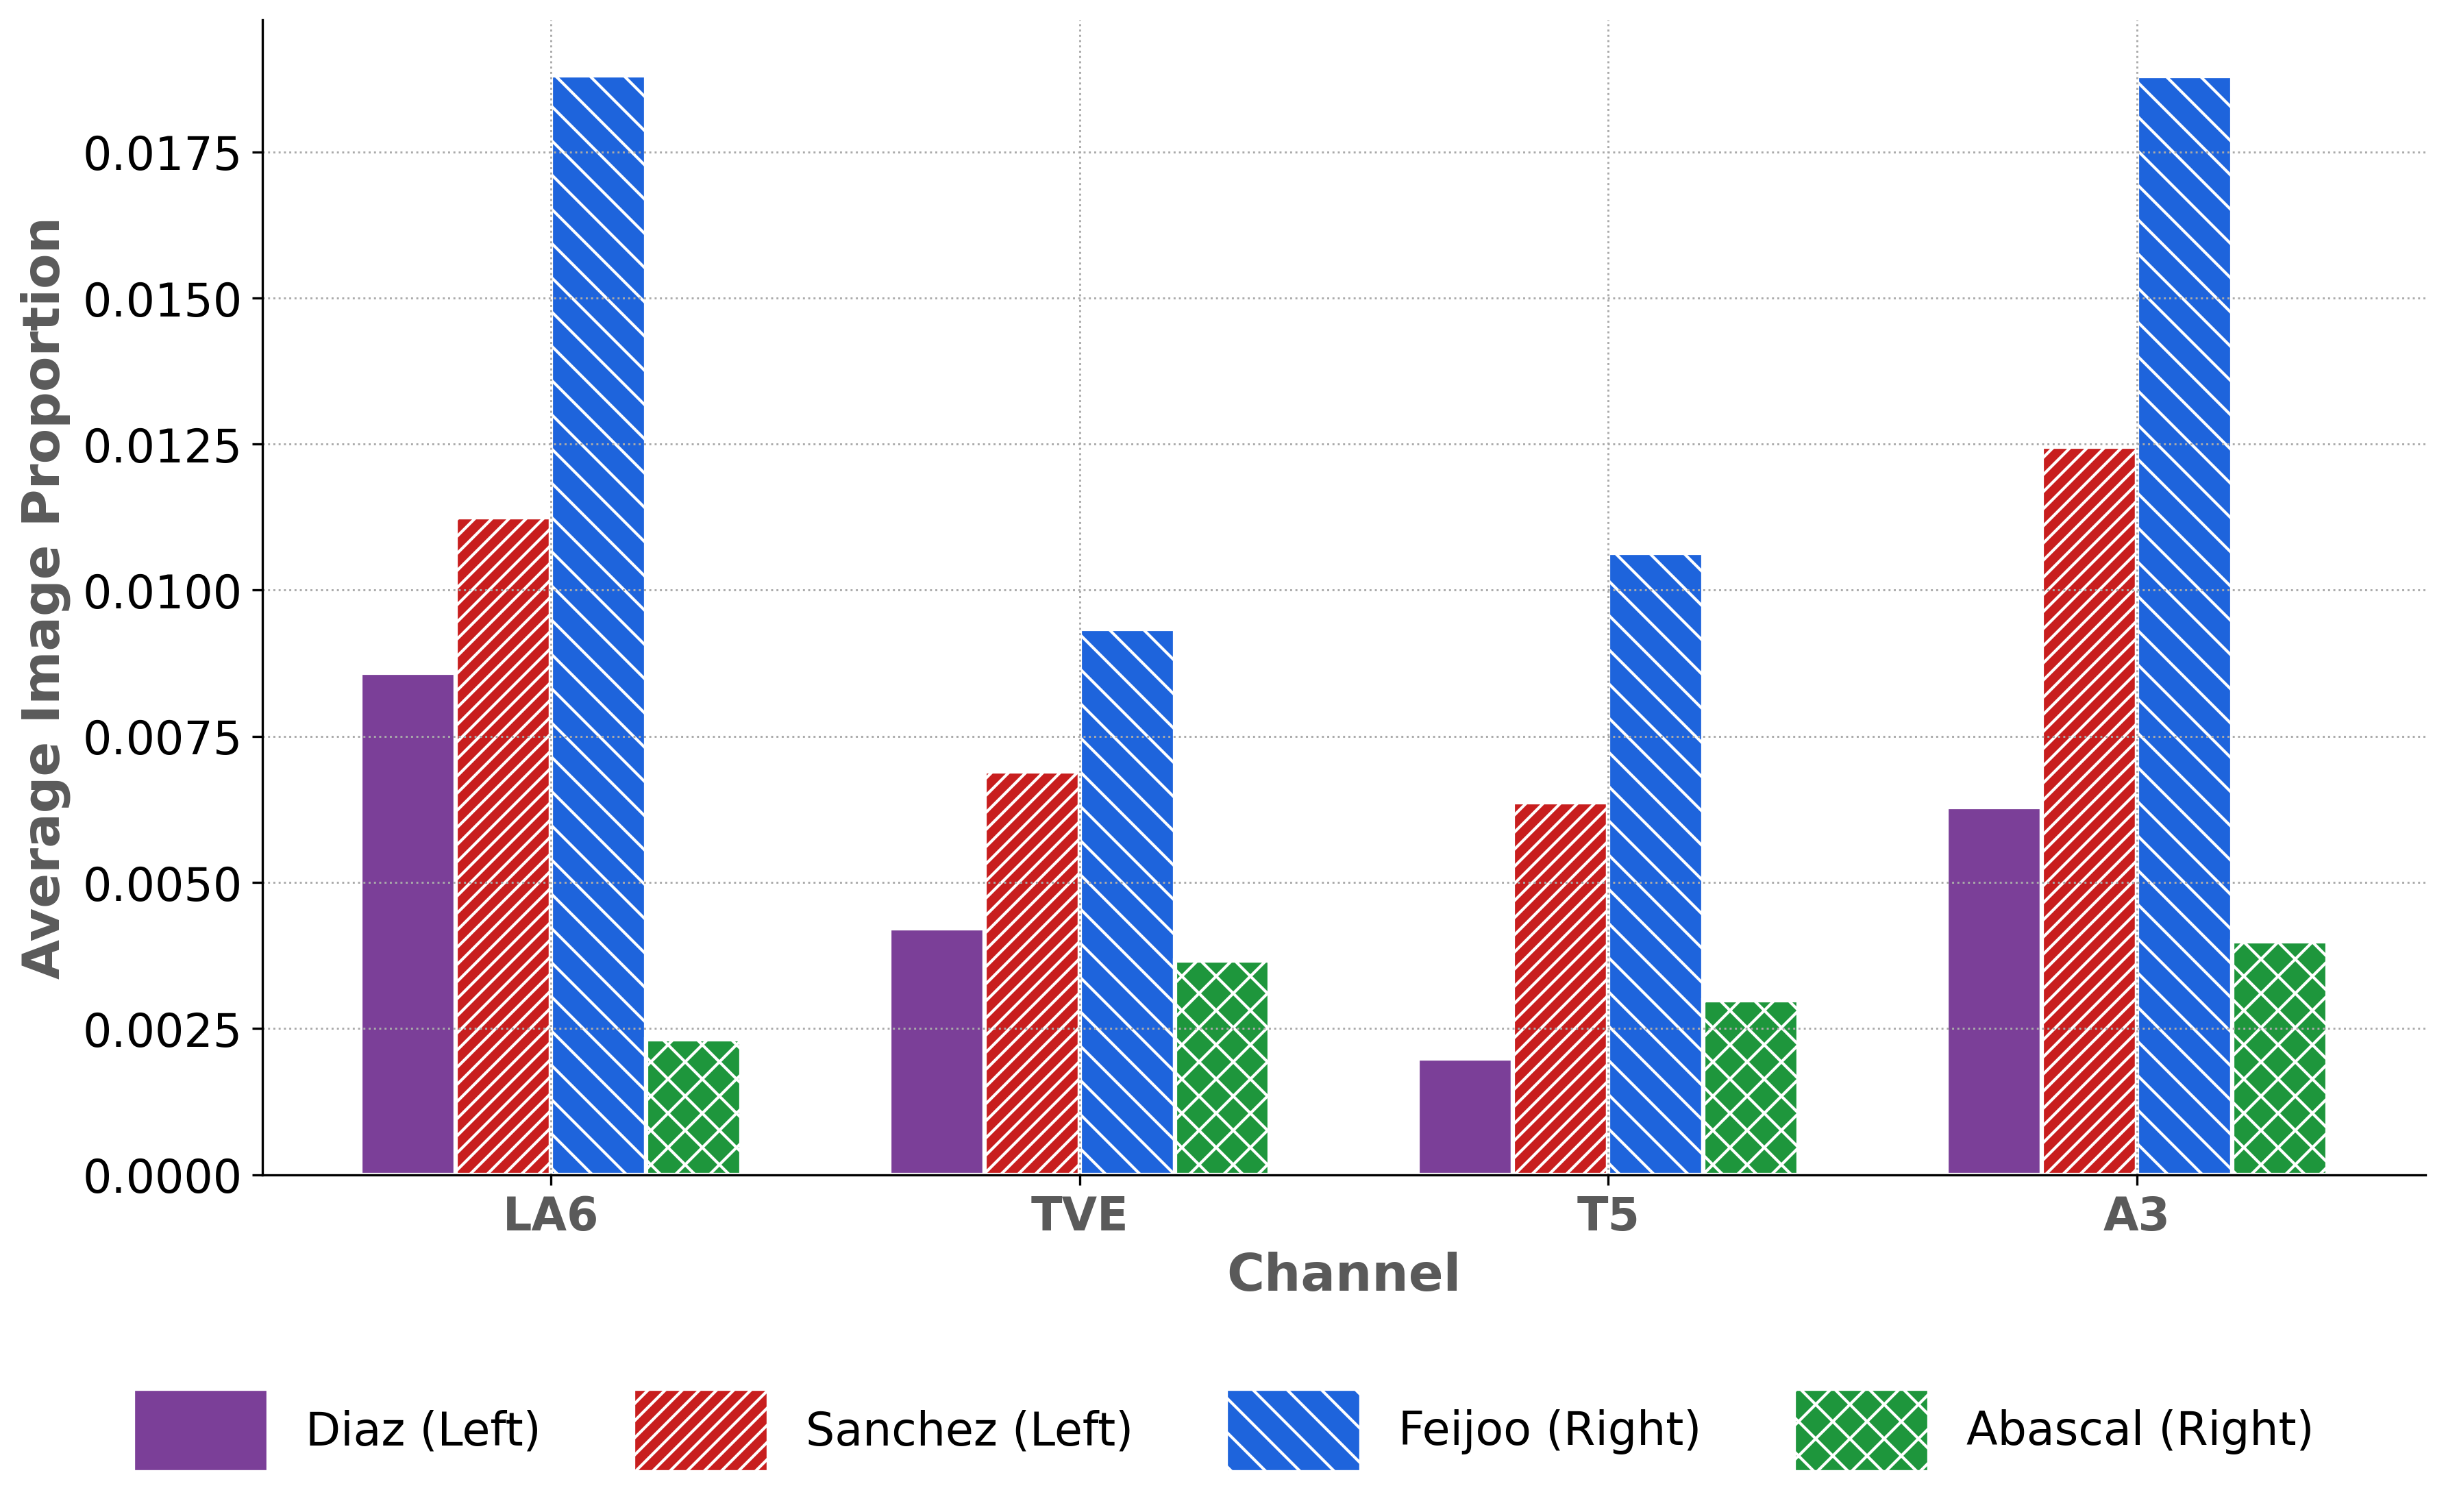
\includegraphics[width=\linewidth]{figures/politicians_image_proportions}
	\end{minipage}%
	\hfill
	%— Right panel —
	\begin{minipage}{0.48\textwidth}
		\centering
		\textbf{(b) Text mentions}\\[1ex]
		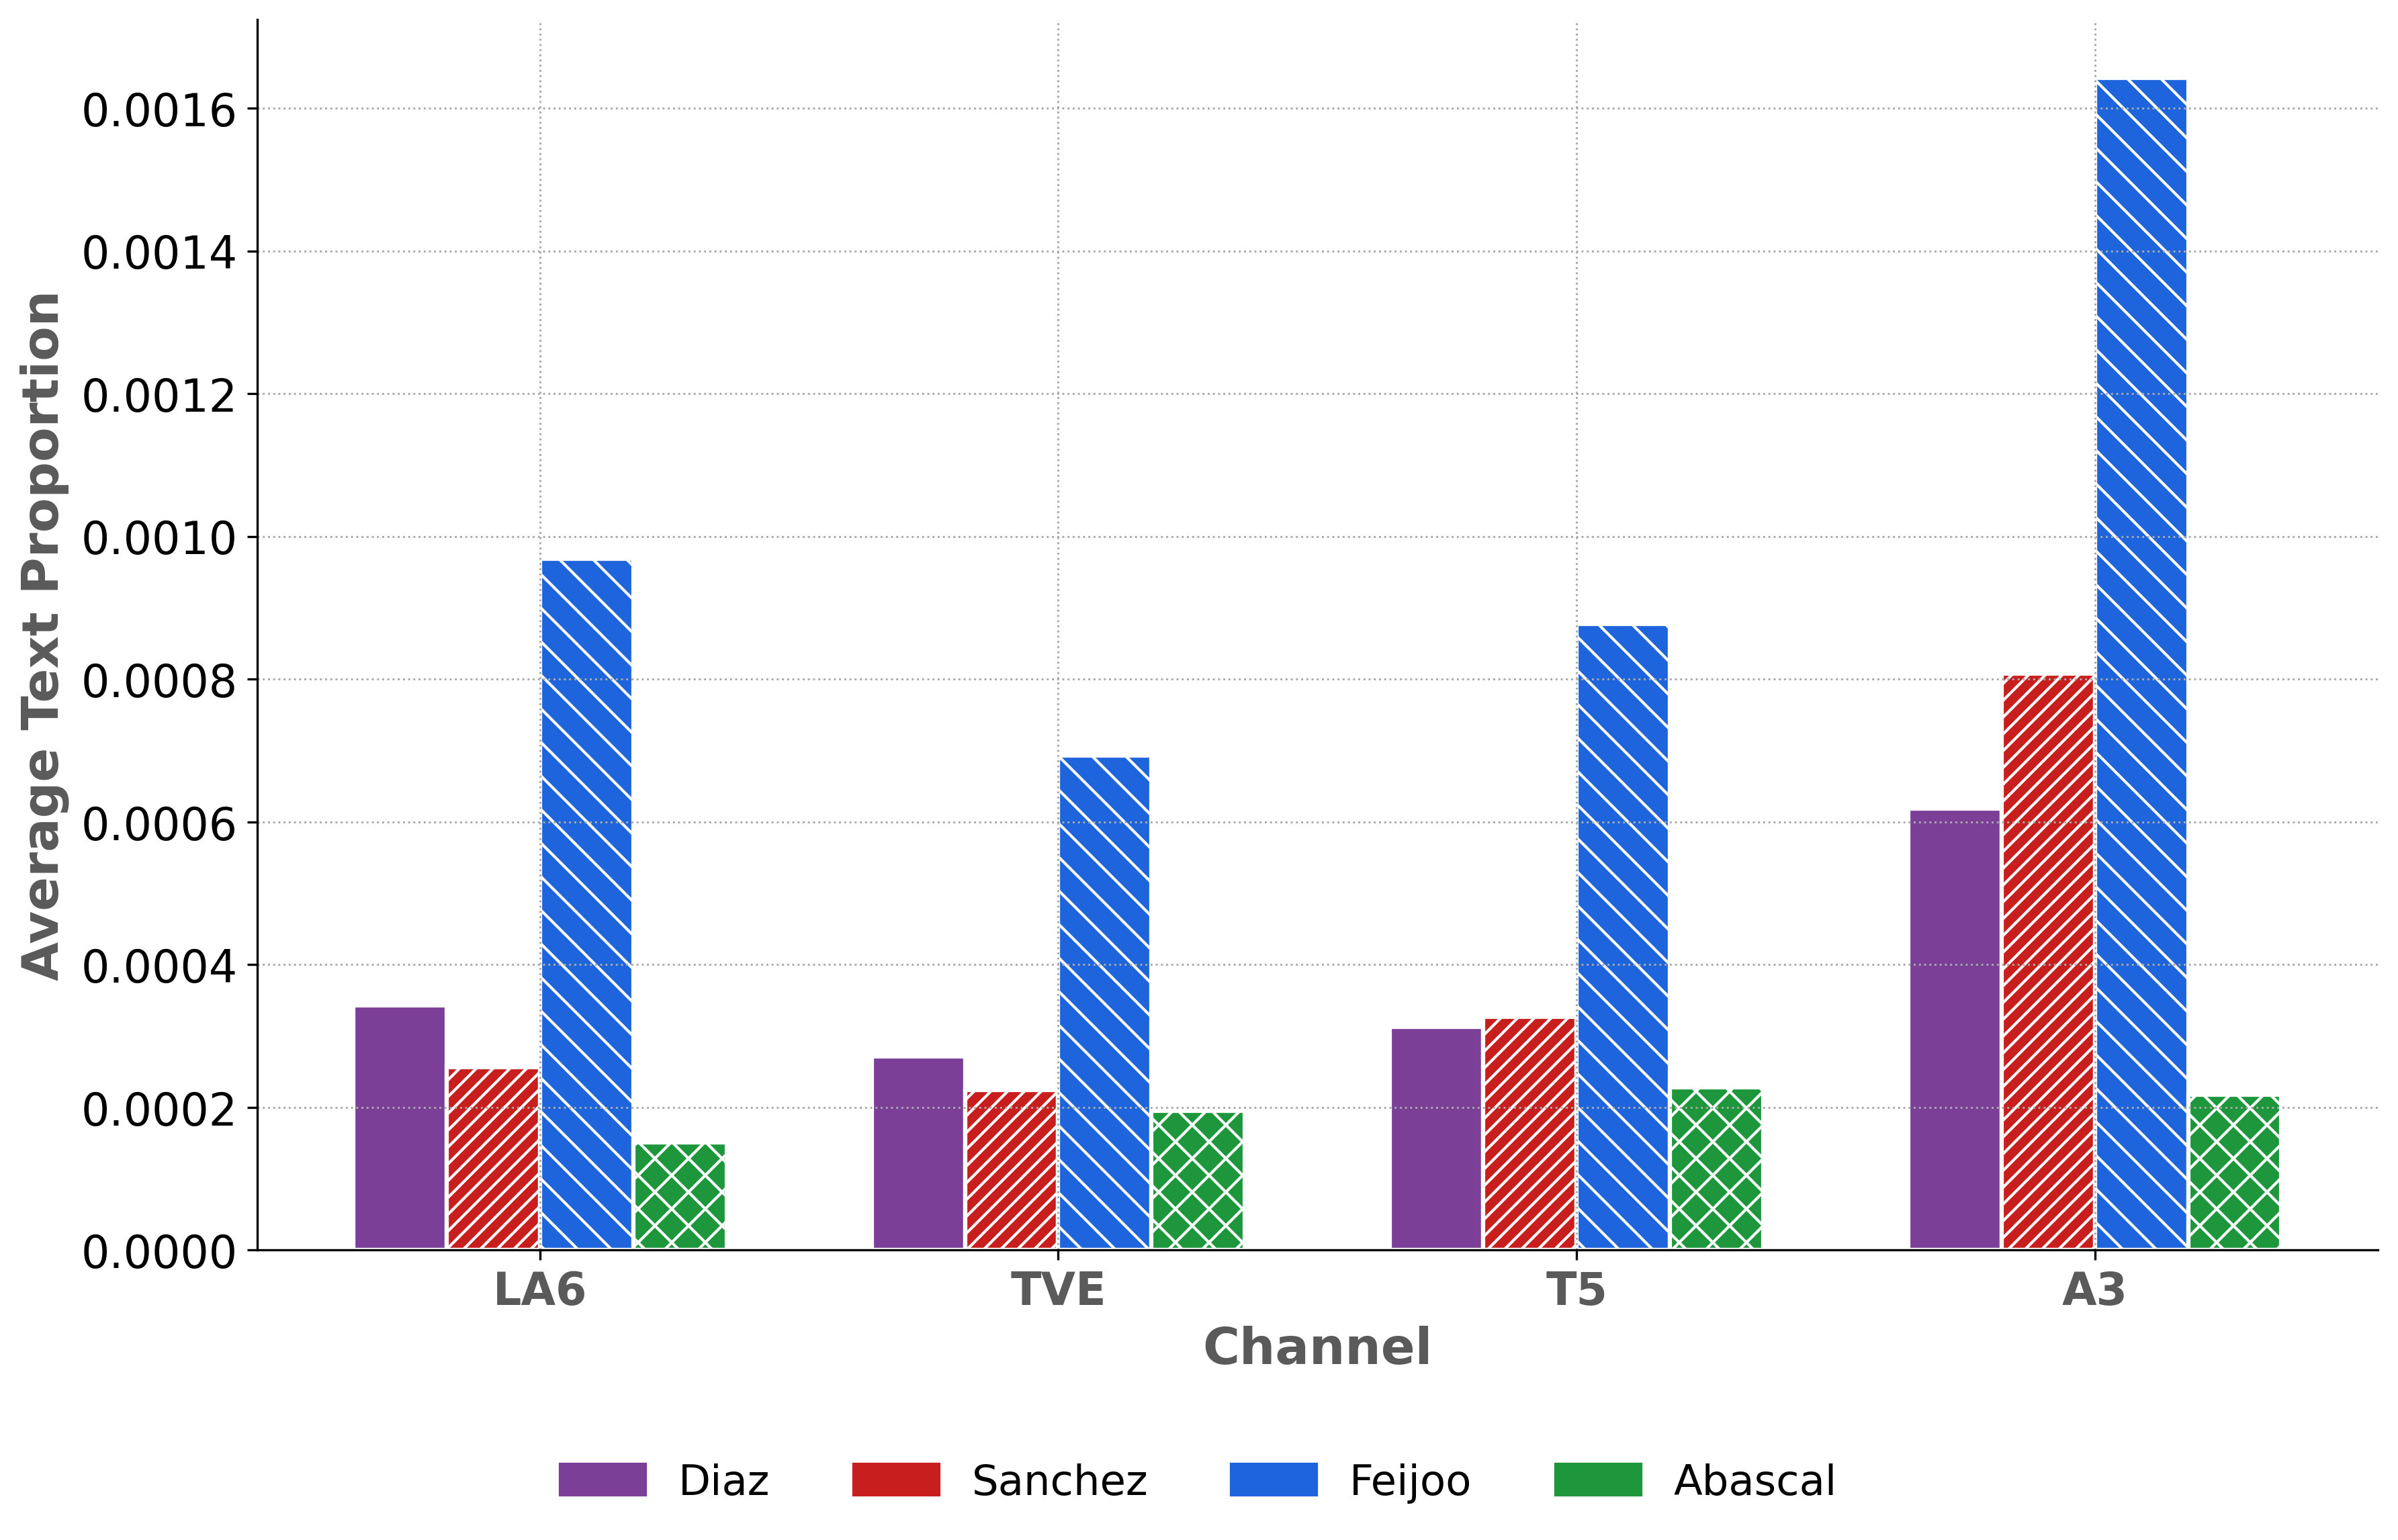
\includegraphics[width=\linewidth]{figures/politicians_text_proportions}
	\end{minipage}
	
	\vspace{1ex}
	
	{\small
		\textit{Note:} The proportions are computed per channel and political actor over the same random sample of 67 days.}
	\label{fig:combined_channel}
\end{figure}



To further examine the relationship between tone—based on the LLM classification—and coverage, I regress net tone by political actor on both the proportion of image appearances and word mentions. Table \ref{tab:images2} reports results under different specifications, including date and channel fixed effects.




\begin{table}[htbp!]
	\centering
	
	\caption{Effect of Mentions on Tone toward Party Leaders}
	\label{tab:images2}
	\small
	\setlength{\tabcolsep}{4pt}
	\renewcommand{\arraystretch}{1.0}
	\begin{tabular}{lcccc}
		\toprule
		& \multicolumn{4}{c}{\textit{Outlet Slant} (\(x\))} \\
		\cmidrule(lr){2-5}
		& (1) & (2) & (3) & (4) \\
		\midrule
		
		\multicolumn{5}{l}{\textbf{Feijóo (PP)}}\\
		Text Mentions     &  -1.956         &  -3.038         &   0.364         &   -1.342        \\
		&  (2.063)        &  (2.134)        &  (2.391)        &  (2.584)        \\
		Image Appearances &  -0.065         &   0.003         &  -0.275         &  -0.189         \\
		&  (0.147)        &  (0.151)        &  (0.179)        &  (0.189)        \\
		\addlinespace
		\hline
		\multicolumn{5}{l}{\textbf{Abascal (VOX)}}\\
		Text Mentions     & -42.813& -44.024& -46.659& -49.989\\
		&  (7.855)        &  (7.832)        &  (9.609)        &  (9.471)        \\
		Image Appearances &   0.963 &   0.933&   0.565         &   0.437         \\
		&  (0.470)        &  (0.470)        &  (0.600)        &  (0.595)        \\
		\addlinespace
		\hline
		\multicolumn{5}{l}{\textbf{Sánchez (PSOE)}}\\
		Text Mentions     &   4.131         &  11.634 &   2.648         &  13.515  \\
		&  (6.020)        &  (6.992)        &  (6.494)        &  (7.909)        \\
		Image Appearances &   0.023         &  -0.045         &   0.033         &   0.032         \\
		&  (0.239)        &  (0.244)        &  (0.356)        &  (0.377)        \\
		\addlinespace
		\hline
		\multicolumn{5}{l}{\textbf{Díaz (UP)}}\\
		Text Mentions     &  -0.576         &   1.276         &  -0.714         &   3.365         \\
		&  (3.158)        &  (3.280)        &  (4.080)        &  (4.405)        \\
		Image Appearances &   0.473&   0.485 &   0.290         &   0.321         \\
		&  (0.197)        &  (0.206)        &  (0.232)        &  (0.247)        \\
		\midrule
		Channel FE        & No              & Yes             & No              & Yes             \\
		Date FE           & No              & No              & Yes             & Yes             \\
		\midrule
		Observations      & 231             & 231             & 231             & 227             \\
		\bottomrule
	\end{tabular}
	
	\vspace{0.5em}
	\begin{flushleft}
		\scriptsize\emph{Note:} Robust standard errors in parentheses;\quad 
		%\sym{*} \(p<0.05\), \sym{**} \(p<0.01\), \sym{***} \(p<0.001\).  
		Each block shows coefficients from regressing net tone on text mentions and image appearances of the party leader.
	\end{flushleft}
\end{table}



Column~(4) reports the specification with both channel and day of the week fixed effects, so the coefficients reflect pure within–channel–day fluctuations in coverage. The pattern is heterogeneous across politicians. For Abascal (VOX), a one-standard-deviation increase in word mentions predicts a decrease of $0.39$ standard deviations in tone, whereas the same increase in on-screen images predicts an increase of $0.06$ standard deviations. Both left-leaning politicians present positive correlations between image appearances and tone, although neither appears to be a strong predictor.

Taken together, the results indicate that text-based and image-based measures of salience relate to tone in systematically different ways. Outlets appear much more homogeneous under this metric, with extreme channels showing similar values. This poses concerns regarding the interpretation of previous metrics based on airtime.




\clearpage


\section{Figures}
	
	
	
	\begin{figure}[!htbp]
		\centering
		\caption{Top Media Source to Acquire Political Information in Spain}
		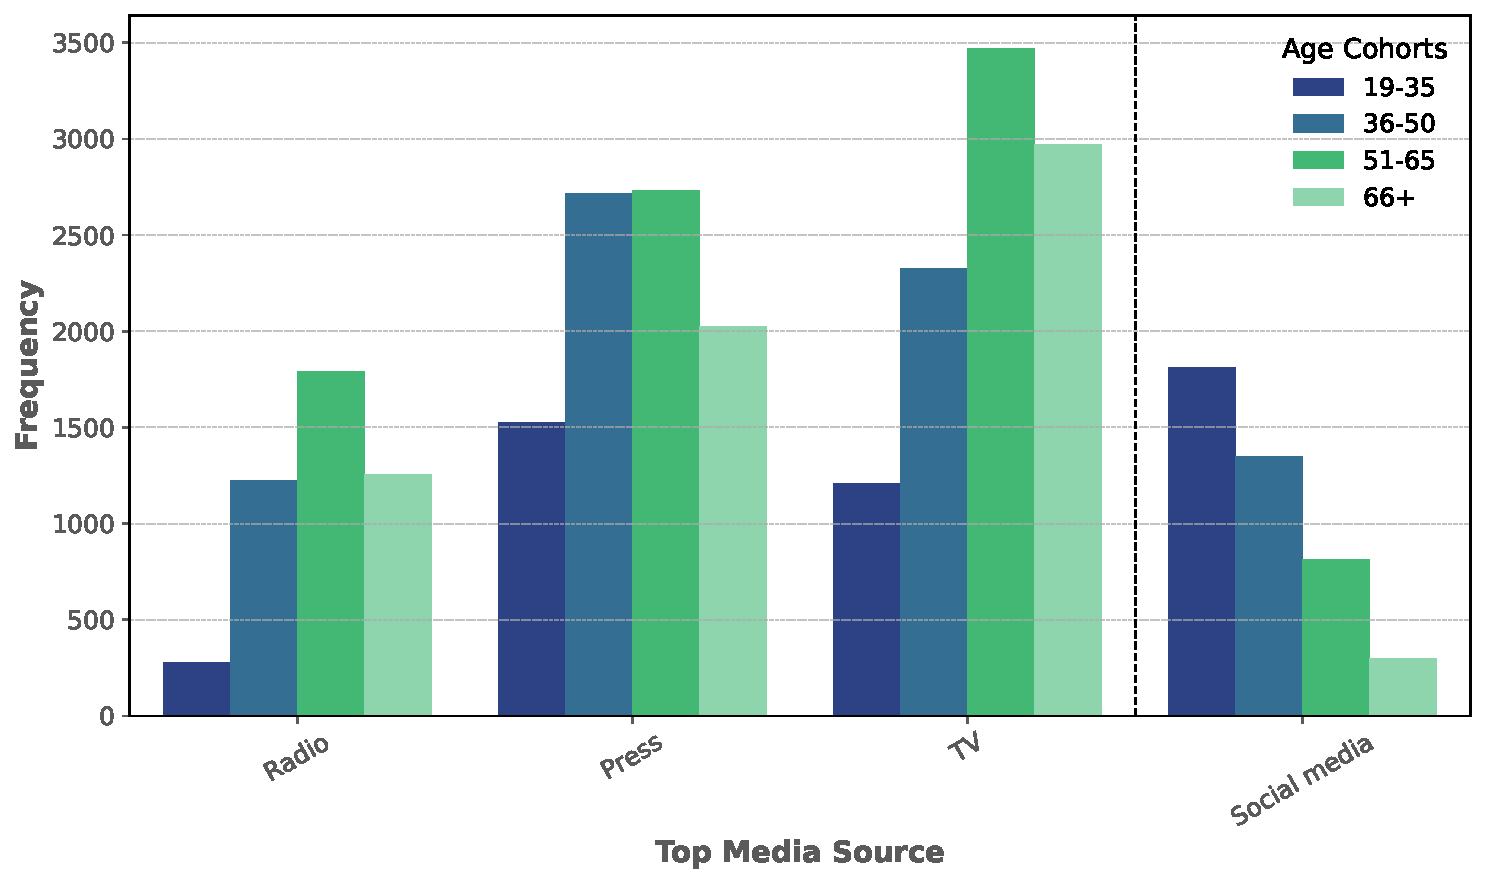
\includegraphics[width=130mm]{figures/age_cohorts}
		\caption*{\small \textit{Note:} Histogram on the preferred media used for political information by age cohorts in Spain.  
			Source: Barómetro CIS, 2023. }
		\label{fig:motivation}
	\end{figure}
	

	
	
	
	\begin{figure}[!htb]
		\caption{Tone across Channels and Parties off and during Campaign }
		\centering
		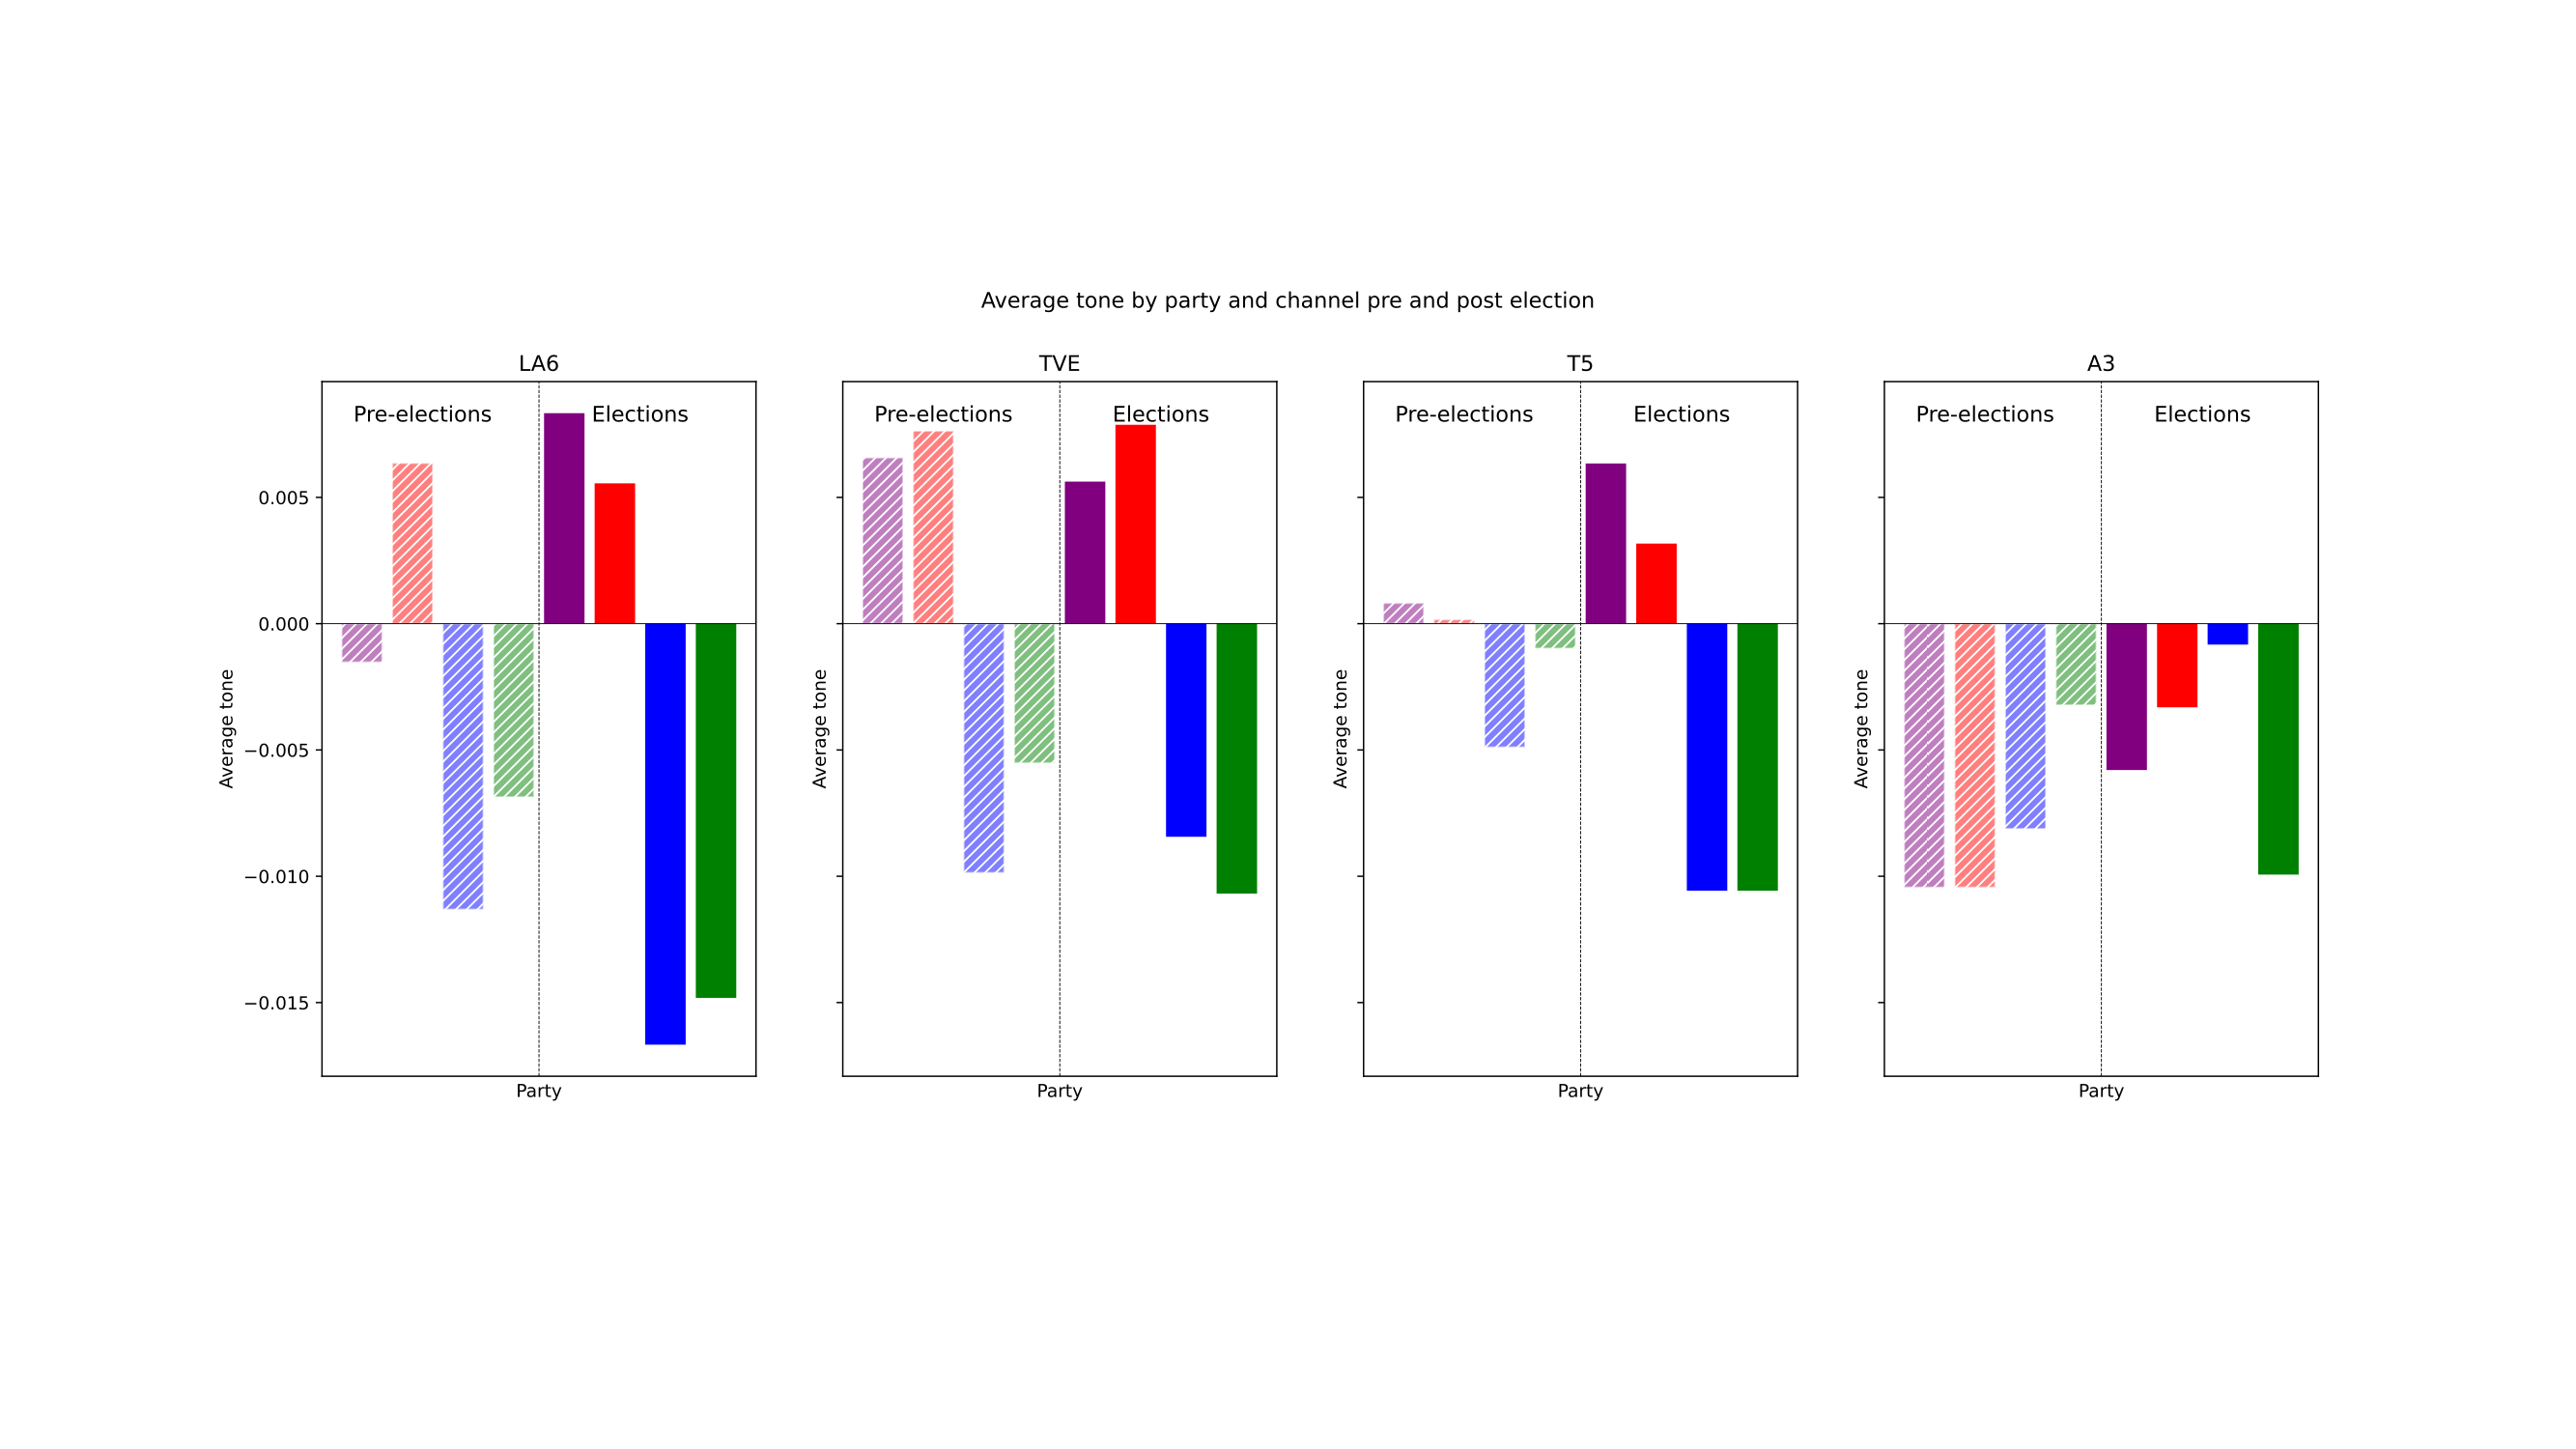
\includegraphics[width=130mm]{figures/average_tone_pre_post_election}
		\caption*{\small \textit{Note:} The figure shows the relative tone calculated as the average sentiment over right and left parties. The vertical dashed line delimits results off and during campaign periods, respectively. }
		\label{fig:tone2}
	\end{figure}
	
	
	
	
	
	\begin{figure}[!htb]
		\caption{Decomposition of Tone across Channels and Parties pre and during Campaign }
		\centering
		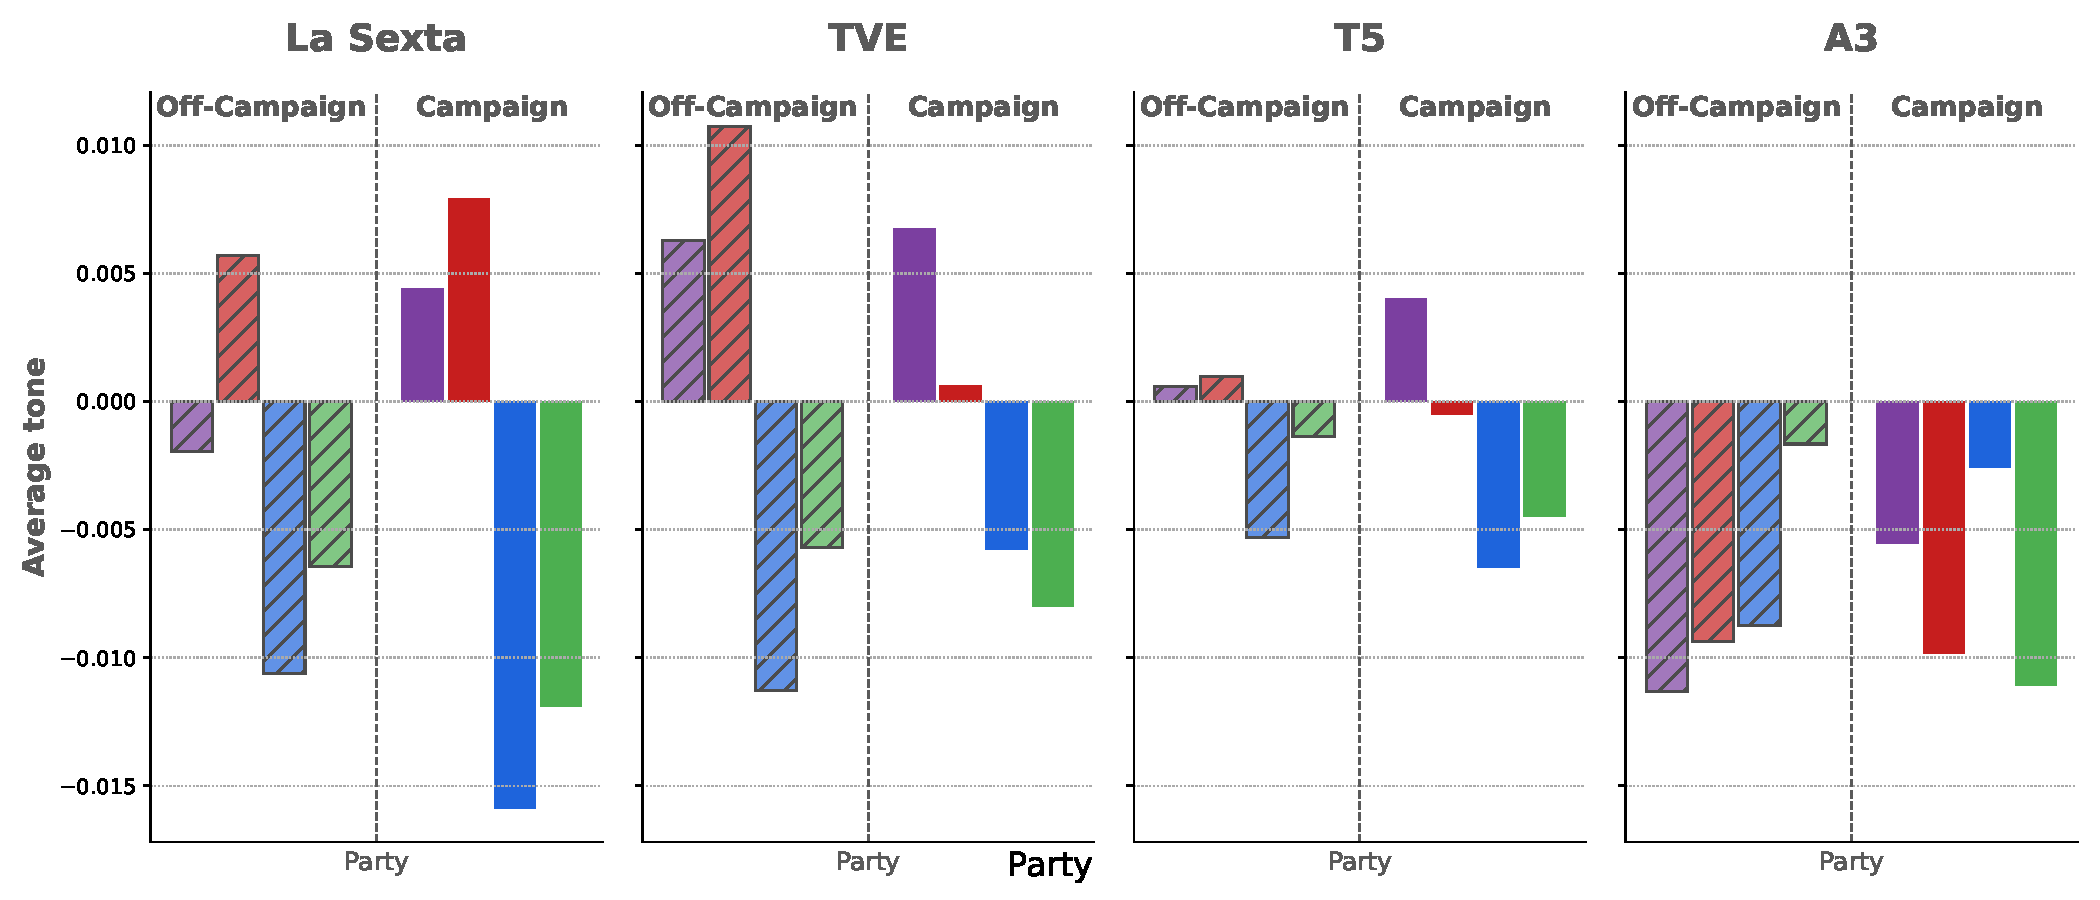
\includegraphics[width=150mm]{figures/average_tone_pre_post_election_party}
		\caption*{\small \textit{Note:} The figure shows the relative tone calculated as the average sentiment over each political party. The vertical dashed line delimits results off and during campaign periods, respectively. }
		\label{fig:tone_by_party}
	\end{figure}
	
	
	\begin{figure}[!htb]
		\caption{Evolution of the Ideological Index by Outlet}
		\centering
		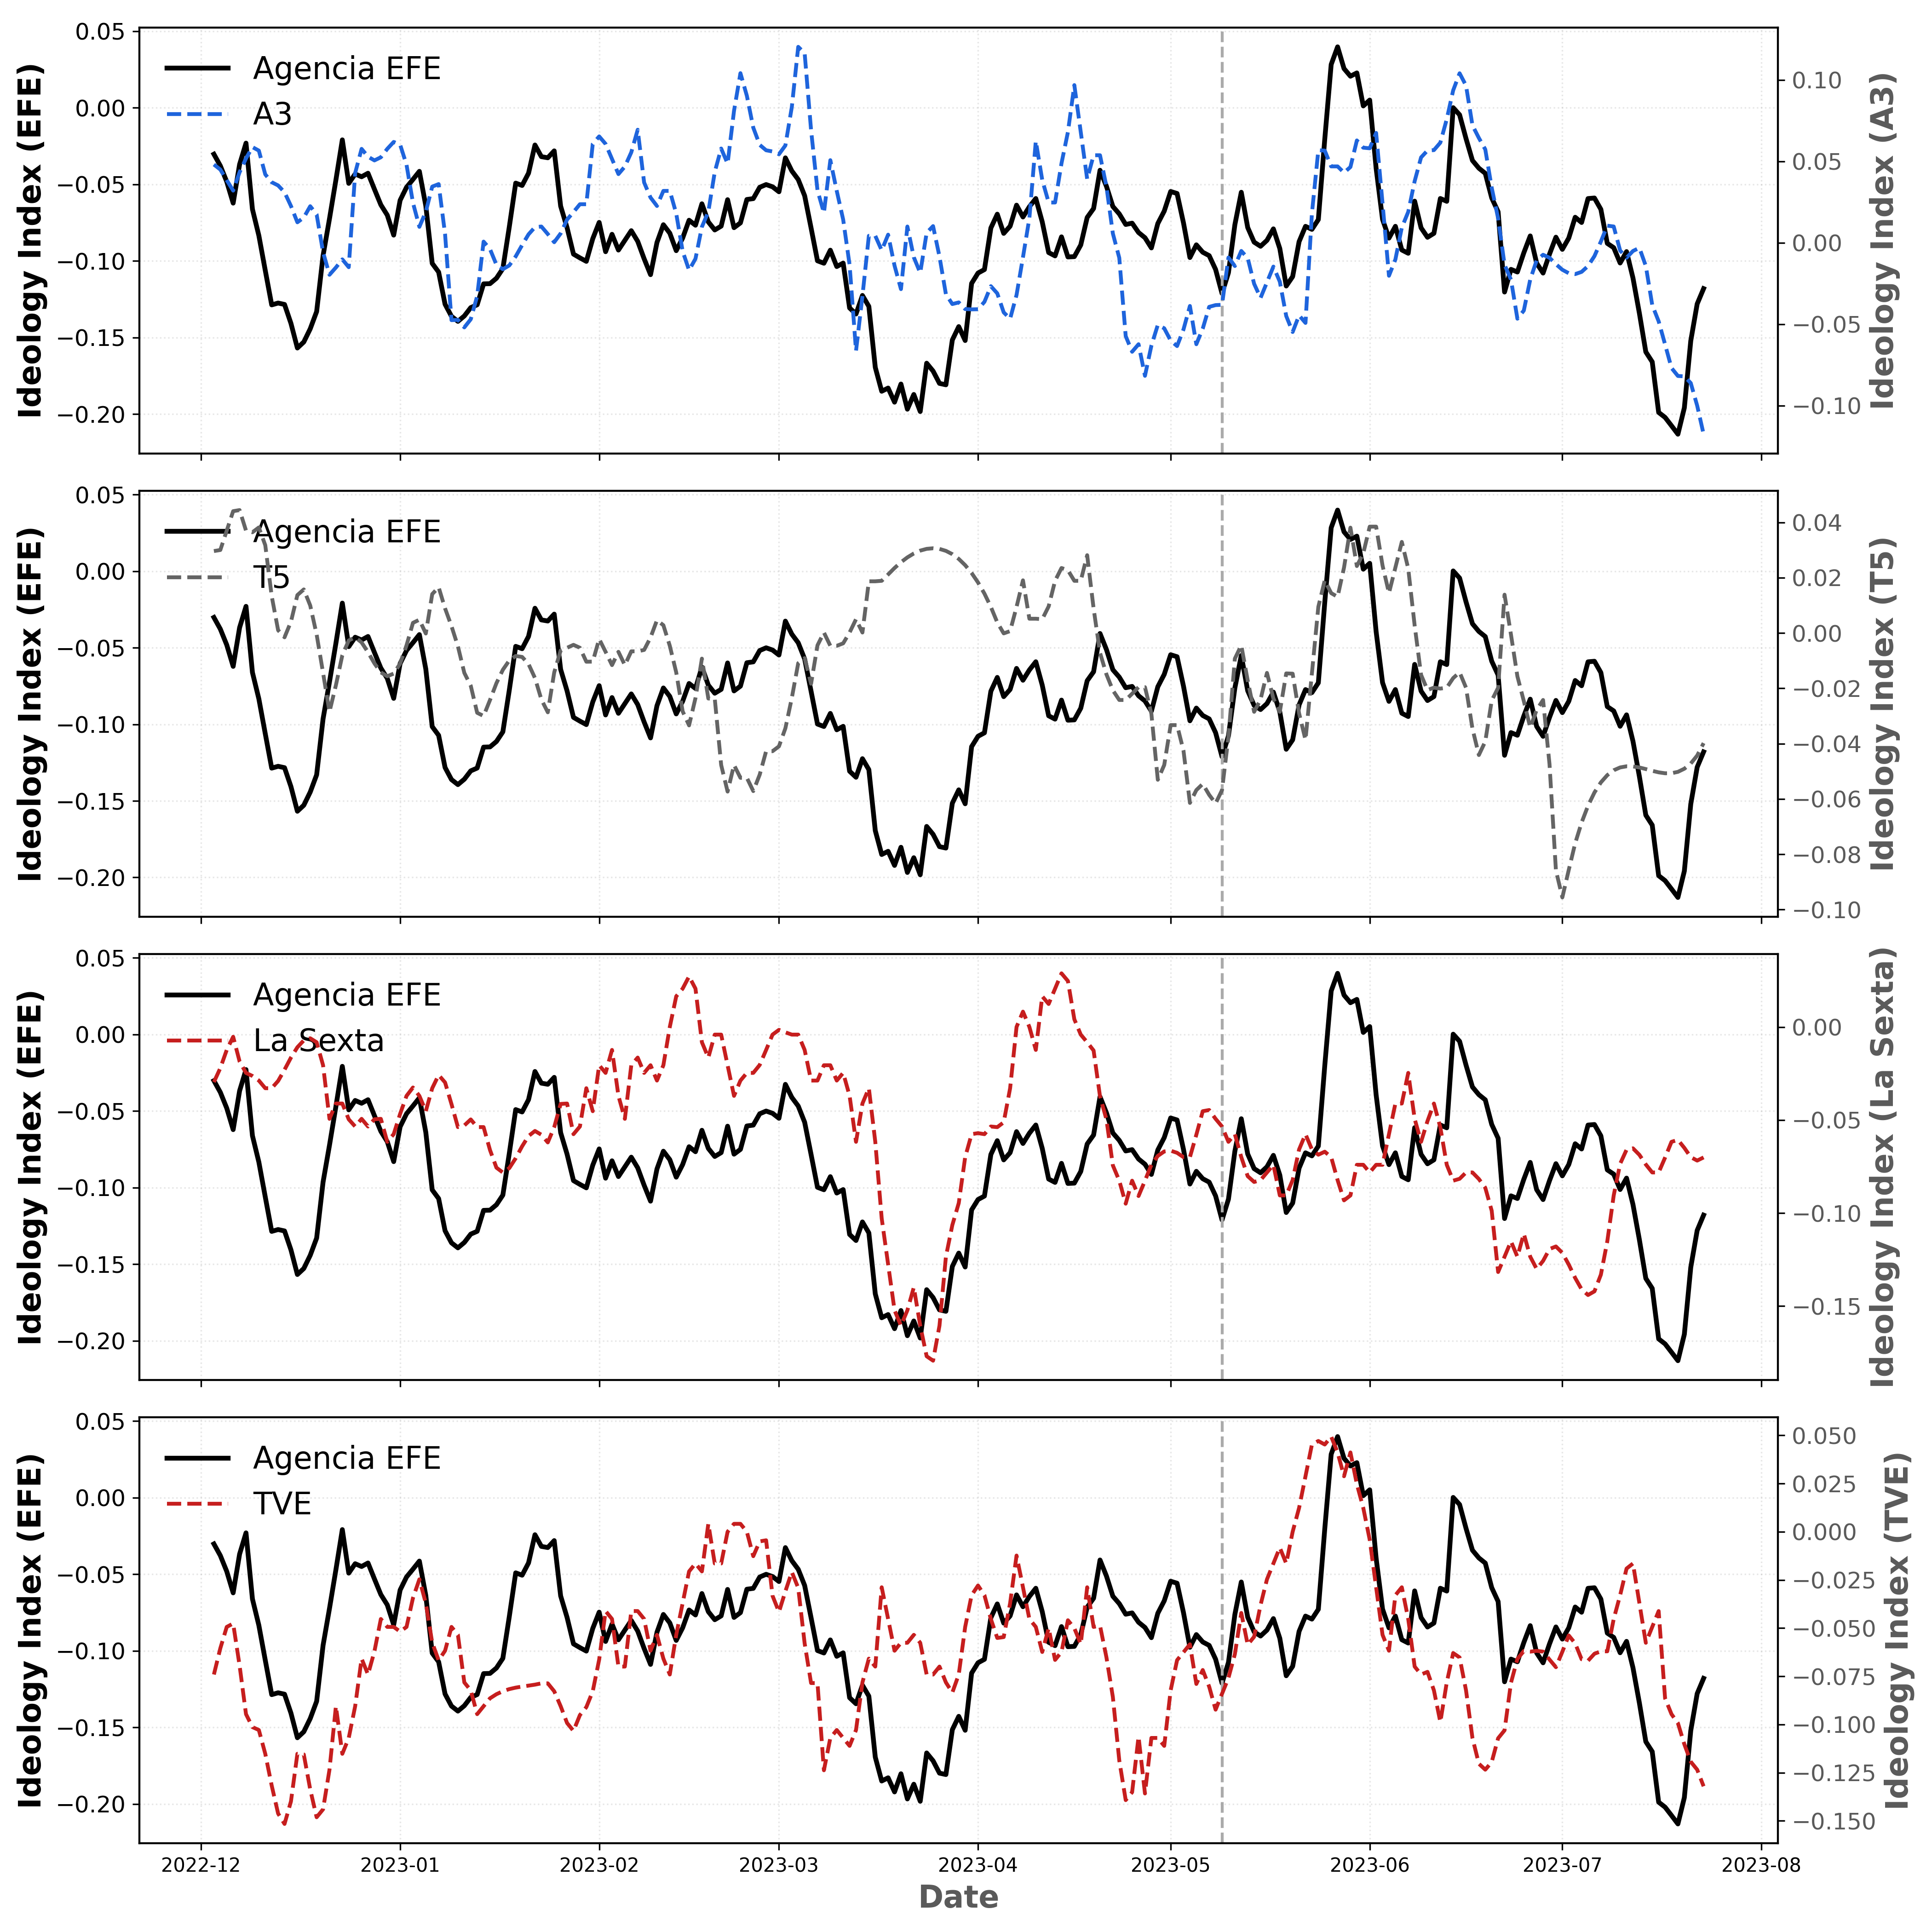
\includegraphics[width=150mm]{figures/tv_vs_efe_net_diff_by_channel}
		\caption*{\small \textit{Note:}The figure represents the smoothed time series of the ideology index in Equation \ref{eq:ideo_index} for TV channels (right y-axis) and the analogous formula for Agencia EFE (solid) on the left axis. The left axis represents the ideological score of the outlets . All series are smoothed using a centered rolling mean with a 9-day window to reduce noise and highlight underlying trends over time.}
		\label{fig:net_tone_by_channel}
	\end{figure}
	
	
	
	
	\begin{comment}
	
	\begin{figure}[H]
		\centering
		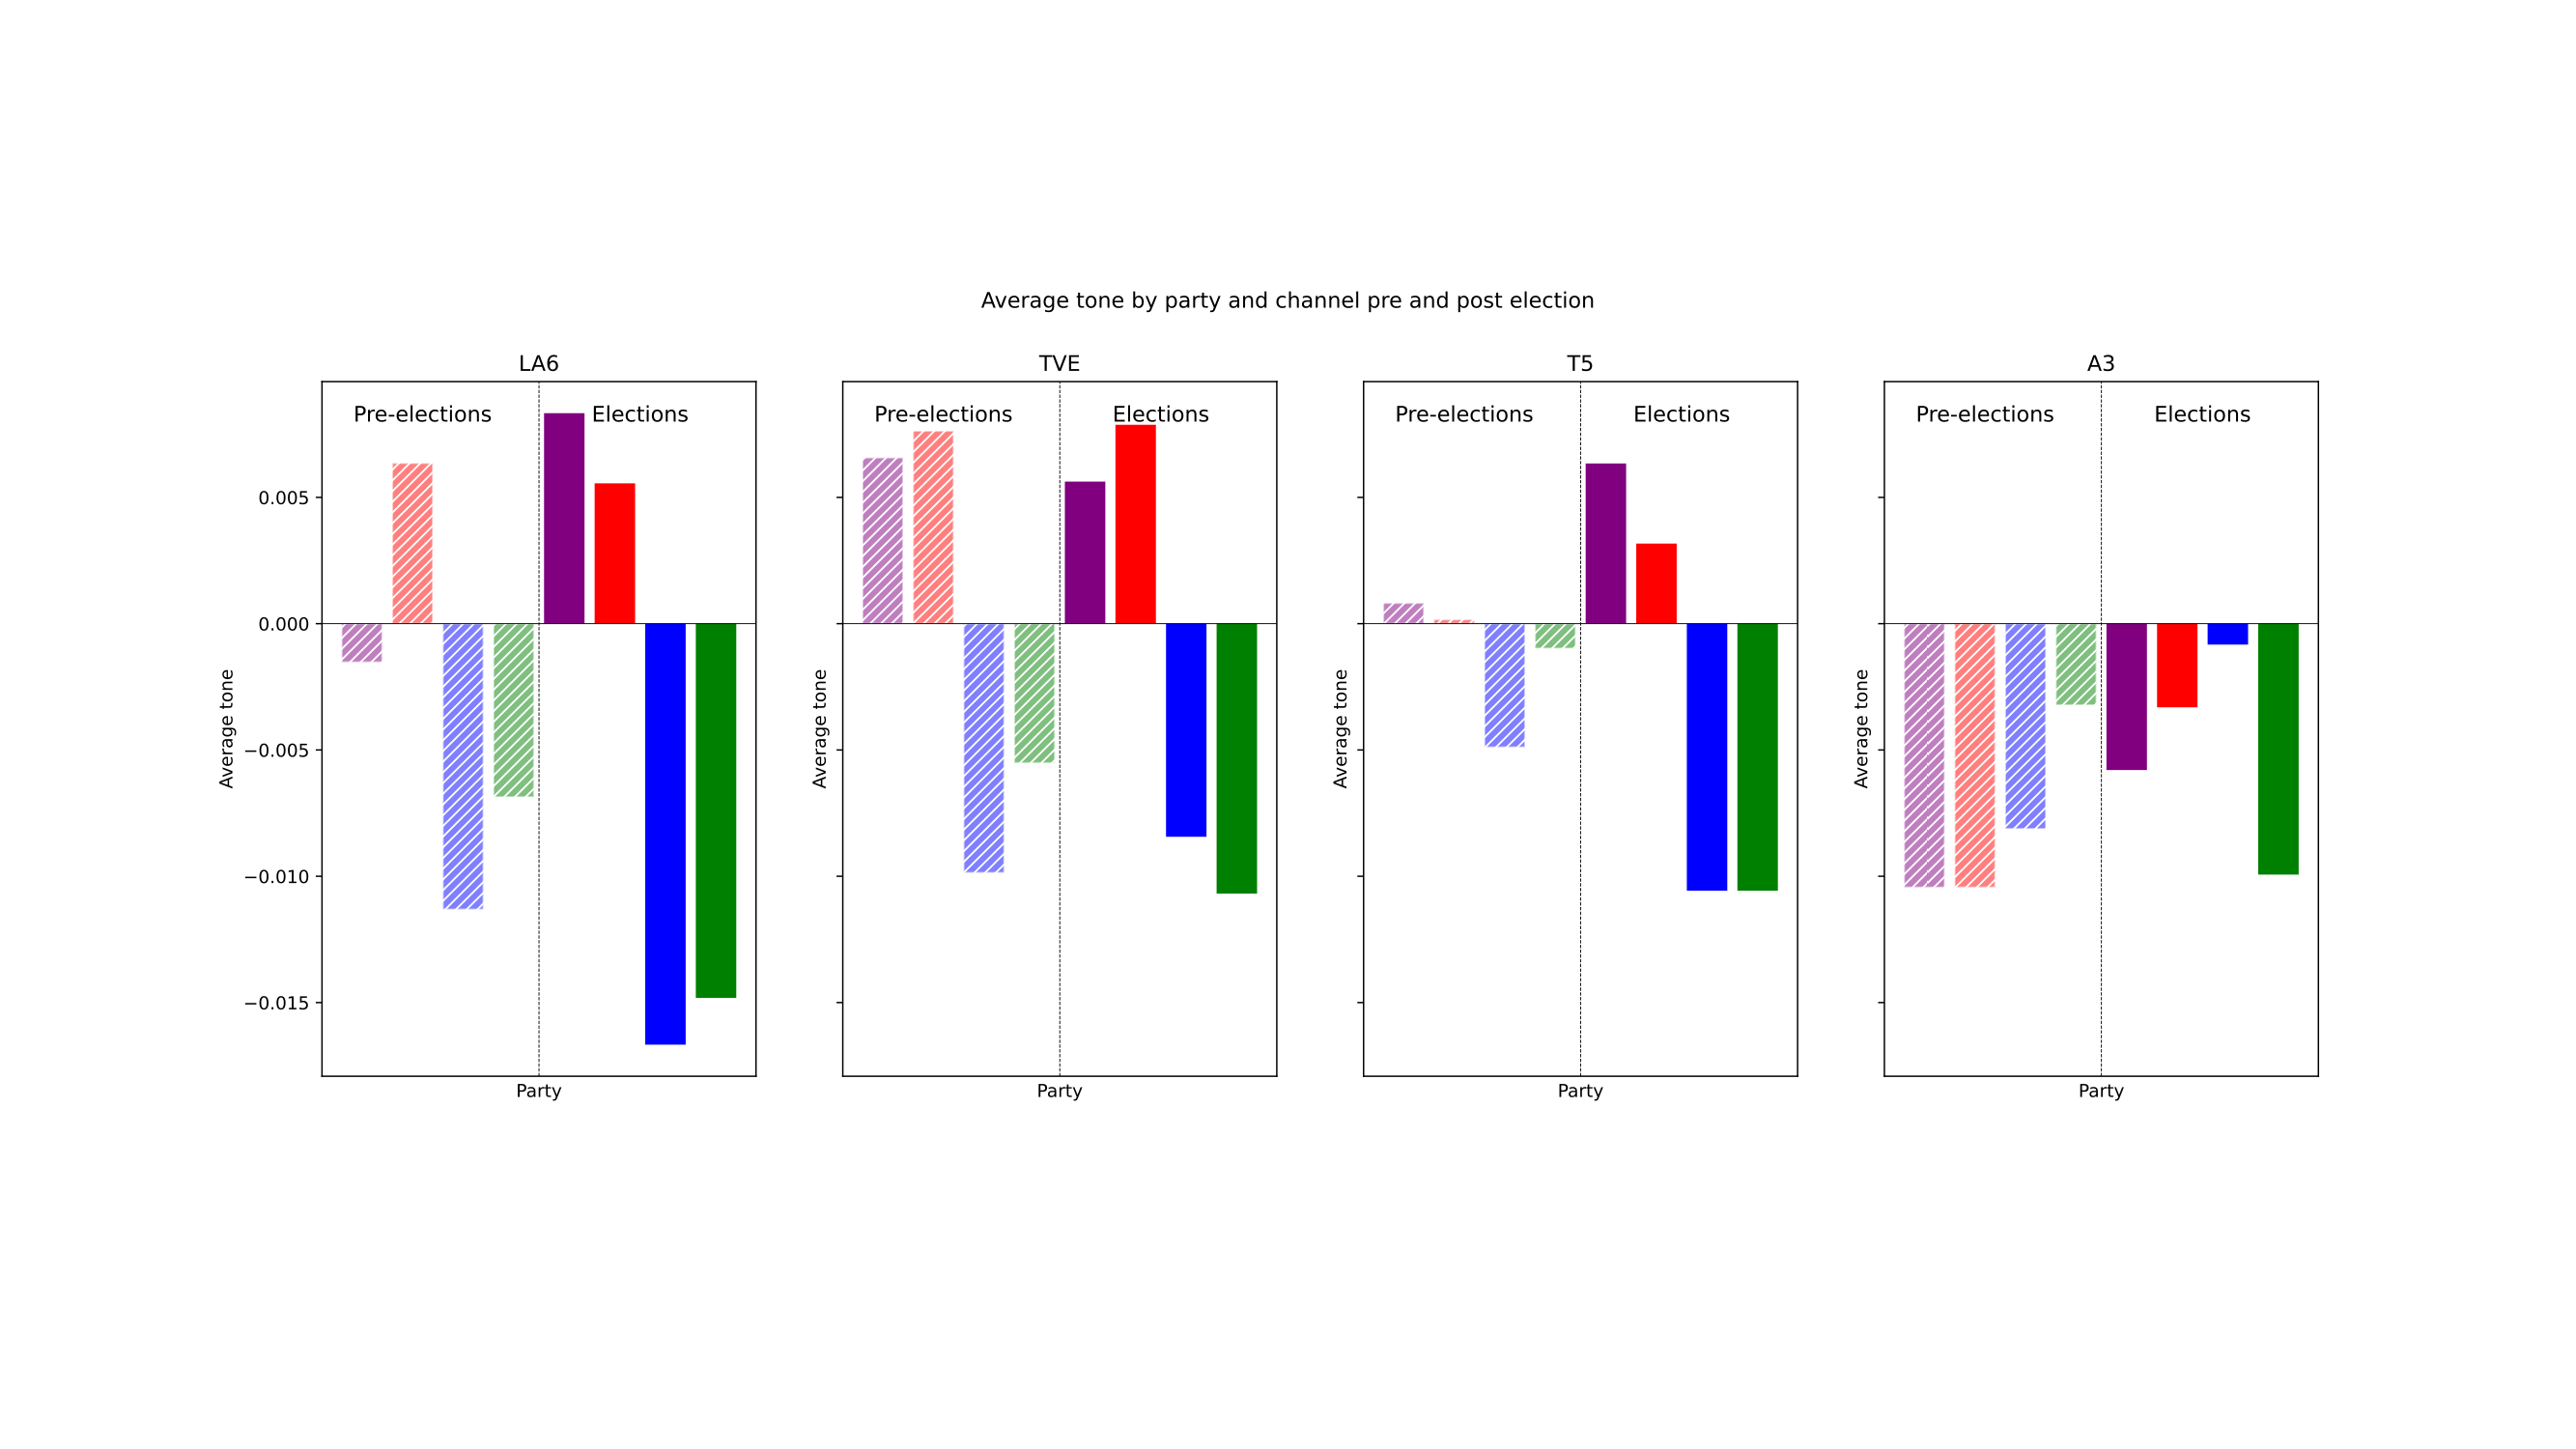
\includegraphics[width=160mm]{figures/average_tone_pre_post_election.png}
		\caption{Average tone for each party and channel pre and during campaign periods}
		\label{fig:party_decomposition}
\end{figure}

		\begin{figure}[h!]
		\caption{Trade-offs in the Model}
		\label{fig:diagram}
		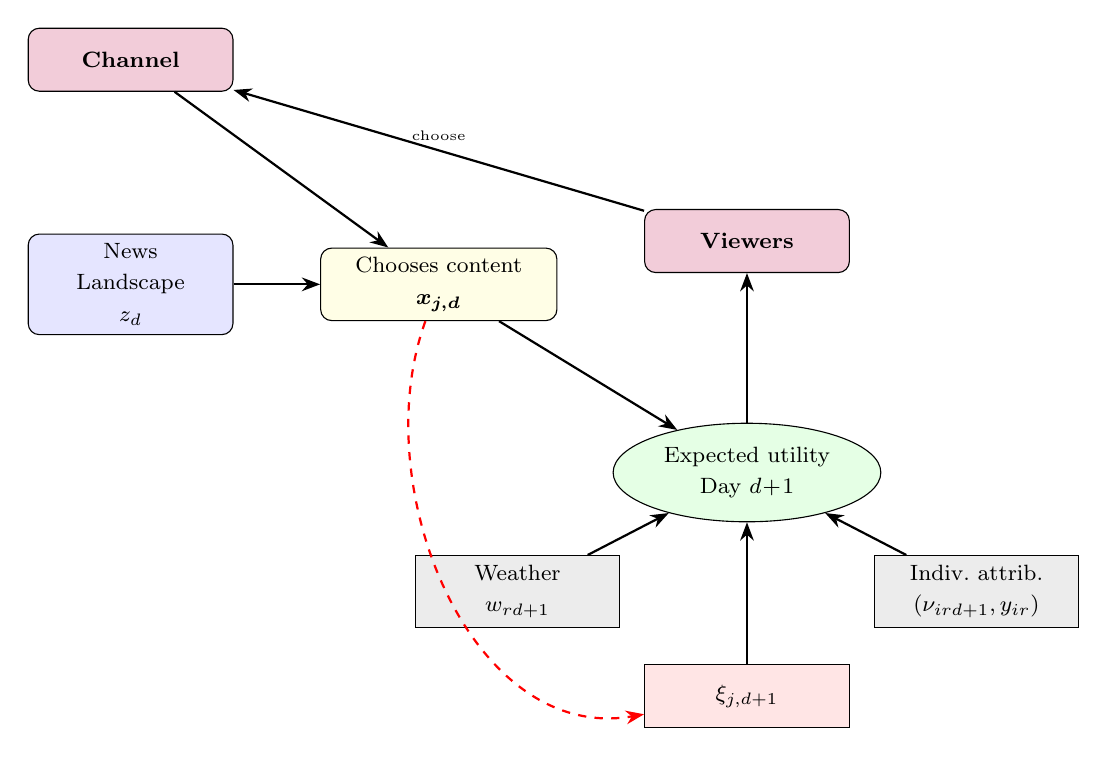
\begin{tikzpicture}[
			inst/.style   ={rectangle, draw, fill=blue!10,  rounded corners, align=center,
				minimum width=2.6cm, minimum height=0.8cm},
			decision/.style={rectangle, draw, fill=yellow!10, rounded corners, align=center,
				minimum width=3.0cm, minimum height=0.9cm},
			util/.style   ={ellipse,   draw, fill=green!10,  align=center,
				minimum width=3.4cm, minimum height=1.0cm},
			shock/.style  ={rectangle, draw, fill=red!10,   align=center,
				minimum width=2.6cm, minimum height=0.8cm},
			exo/.style    ={rectangle, draw, fill=gray!15,  align=center,
				minimum width=2.6cm, minimum height=0.8cm},
			actor/.style  ={rectangle, draw, fill=purple!20, rounded corners, align=center,
				minimum width=2.6cm, minimum height=0.8cm},
			flow/.style   ={-Stealth, thick},
			feed/.style   ={dashed,-Stealth, thick, red},
			node distance = 1.8cm and 1.1cm,
			font=\footnotesize
			]
			% -------- DAY d (supply) ---------
			\node[inst]                    (news)   {News\\Landscape\\$z_{d}$};
			\node[actor, above=of news]    (channel) {\textbf{Channel}};
			
			\node[decision, right=of news] (x)      {Chooses content\\$\bm{x_{j,d}}$};
			
			% -------- DAY d+1 (demand) ------
			\node[actor, right=of x, yshift=0.55cm] (viewer) {\textbf{Viewers}};
			
			\node[util,  below=of viewer, yshift=-0.1cm] (util)
			{Expected utility\\Day $d\!+\!1$};
			\node[shock, below=of util]     (xi)     {$\xi_{j,d+1}$};
			\node[exo,   below left=0.6cm and 0.4cm of util]
			(weather){Weather\\$w_{rd+1}$};
			\node[exo,   below right=0.6cm and 0.4cm of util]
			(prefs)  {Indiv.\ attrib.\\$(\nu_{ird+1},y_{ir})$};
			
			% ---------- flows ---------------
			\draw[flow] (channel) -- (x);
			\draw[flow] (news)    -- (x);
			\draw[flow] (x)       -- (util);
			\draw[flow] (prefs)   -- (util);
			\draw[flow] (weather) -- (util);
			\draw[flow] (xi)      -- (util);
			\draw[flow] (util)    -- (viewer) node[midway,right,font=\tiny]{};
			\draw[flow] (viewer)    -- (channel) node[midway,above,font=\tiny]{choose};
			
			
			% ------ anticipation feedback ---
			\draw[feed] (x) to[out=-110,in=190] node[midway,below,font=\tiny]
			{} (xi);
		\end{tikzpicture}
		\caption*{\small
			\textit{Note:} This diagram illustrates the structure of the model. Solid black arrows indicate causal and temporal dependencies among variables. The red dashed arrow emphasizes the simultaneity problem: content decisions $\bm{x}_{j,d}$ are made with knowledge of the future utility shock $\xi_{j,d+1}$.
		}
		
	\end{figure}
	
		\end{comment}	
	
	\begin{comment}
		content...

	\begin{figure}[ht!]
		\centering
		\caption{Density Estimation for Channels' Ideology (Audience Share)}
		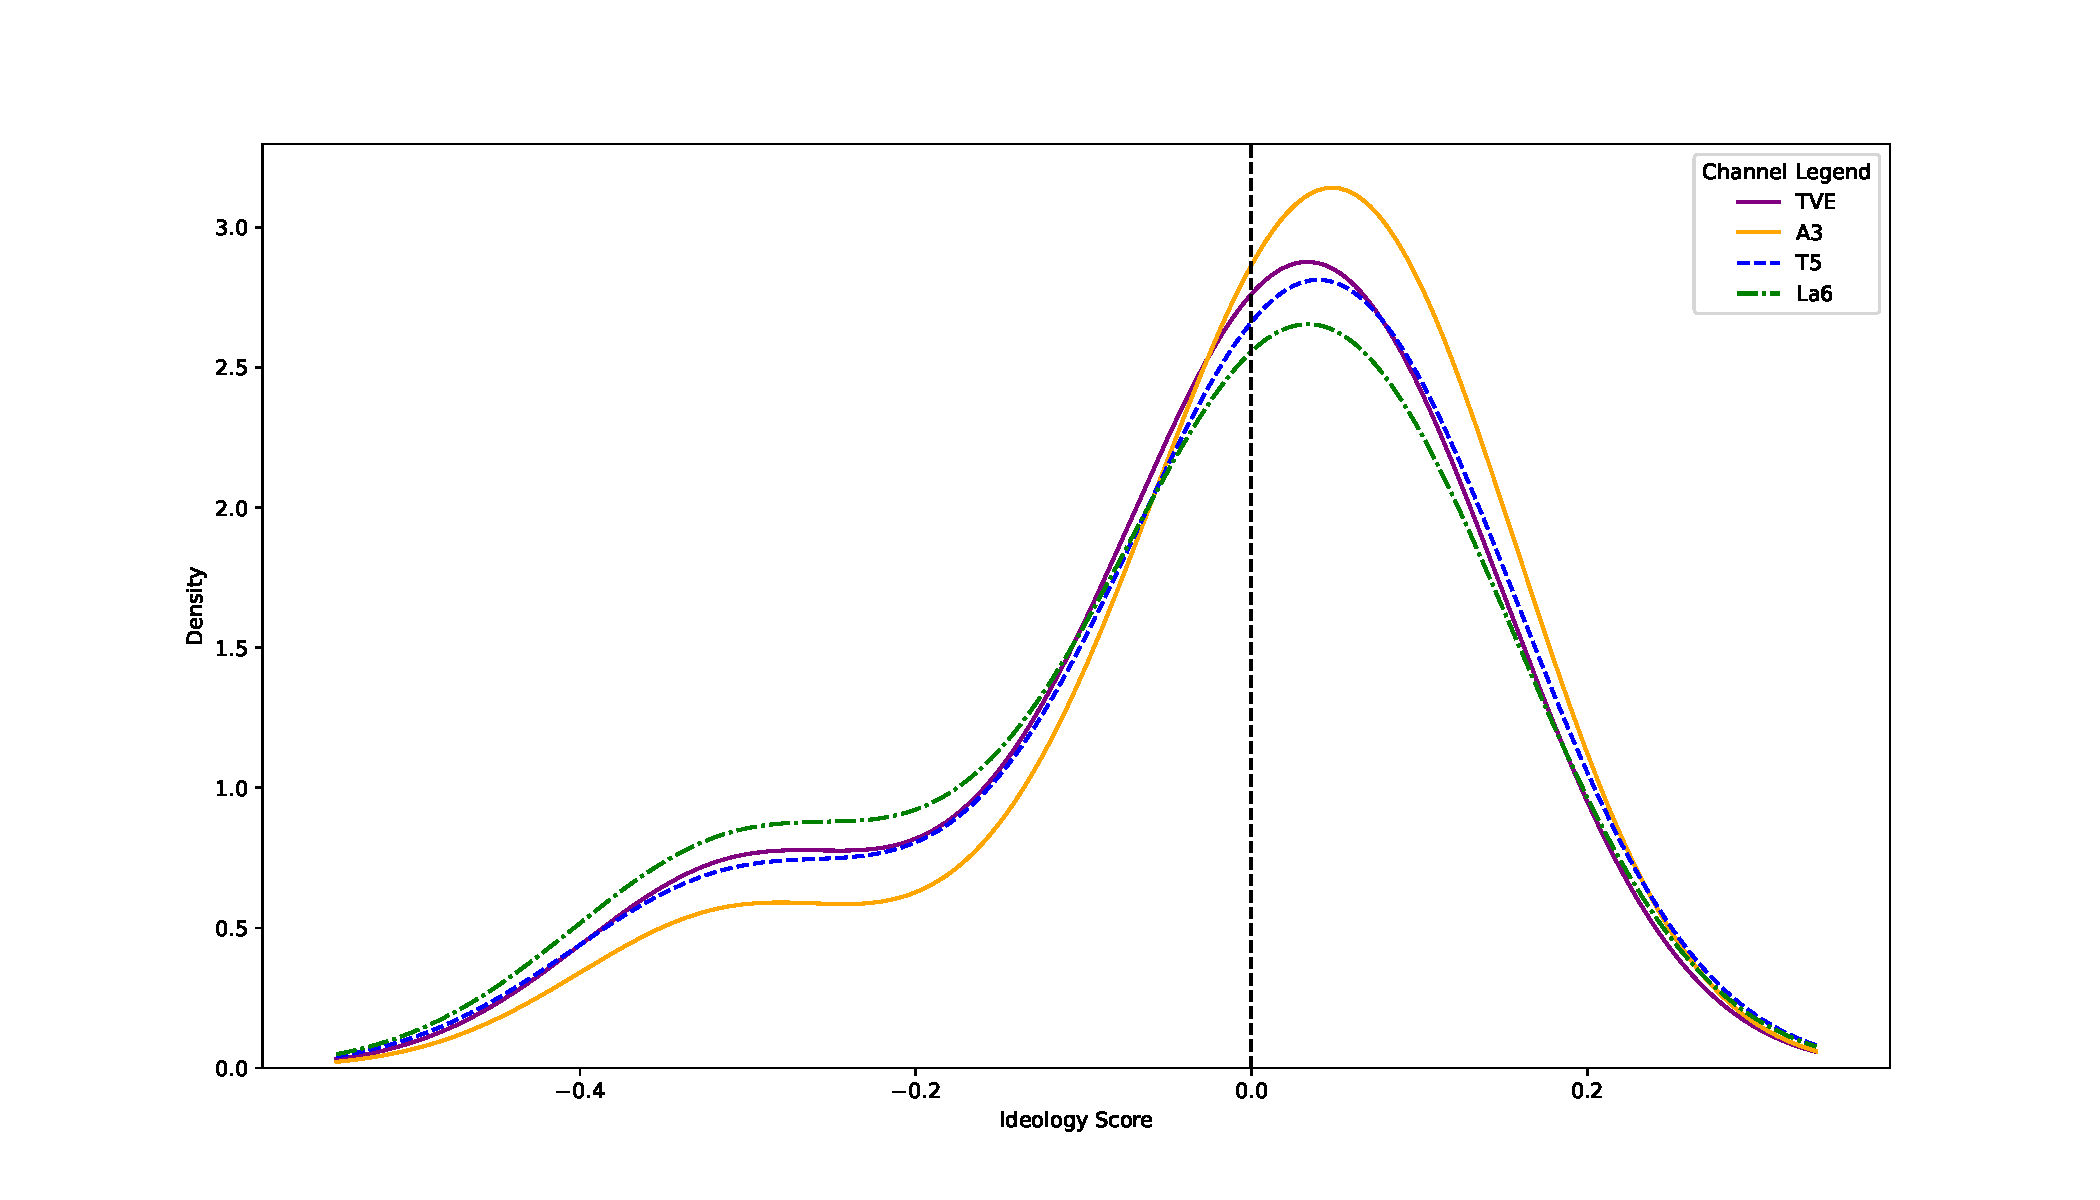
\includegraphics[width=120mm]{figures/channel_ideology_density_python}
		\caption*{\small \textit{Note:} Estimated density of channels' audience ideology. The figure shows a kernel density estimate on the ideology score constructed using survey daa and weighted by channels' share of audience for each autonomous region. }
		\label{fig:density}
	\end{figure}
	
		\end{comment}
		
		\begin{figure}[ht!]
		\centering
		\caption{Added Variable Plots for Production of Political Content (non-parametric fit)}
		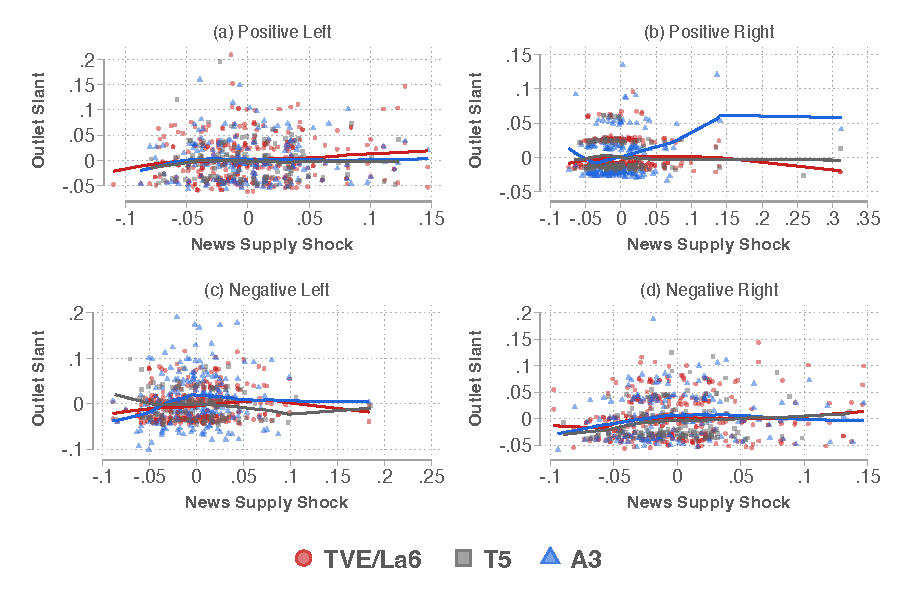
\includegraphics[width=160mm]{figures/fwl_plots_lowess_v2}
		\caption*{\small \textit{Note:} The figure shows the added variable plots from the estimation of equation \ref{eq:first_stage}. The x axis represents $(z_d^{party,+},z_d^{party,-}) $ and the y axis the corresponding  $(x_{jd}^{party,+},x_{jd}^{party,-}) $   . Channels are pooled into left (TVE and La Sexta), middle (Telecinco) and right (A3) for visualization purposes.  }
		\label{fig:fwl_lowess}
	\end{figure}
	

	
	\begin{figure}[!htbp]
		\centering
		\caption{Estimated Elasticities for Left and Right markets off-Campaign}
		\label{fig:elasticities_pre}
		\vspace{0.5em} % space between caption and figures
		
		\begin{minipage}{0.45\textwidth}
			\centering
			\textbf{(a)} Left Markets\\
			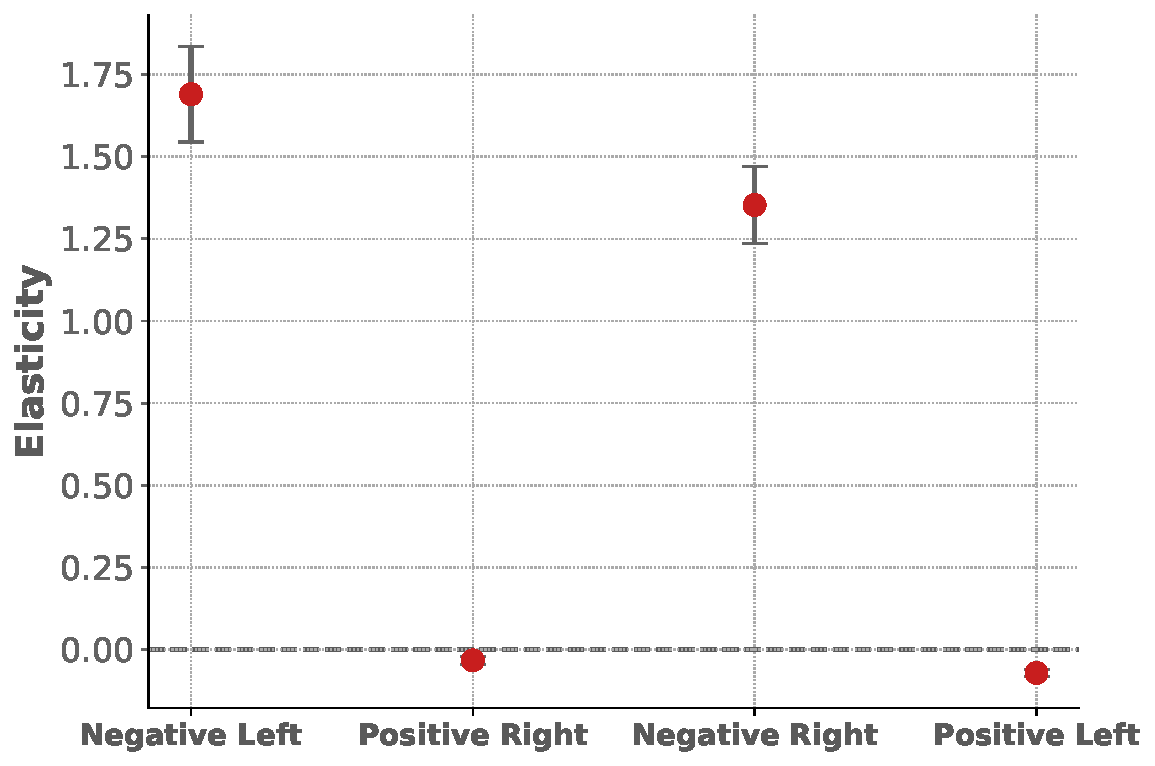
\includegraphics[width=\linewidth]{figures/elasticities_left_pre}
			%		\label{fig:2figsA}
		\end{minipage}
		\hfill
		\begin{minipage}{0.45\textwidth}
			\centering
			\vspace{1.5em}
			\textbf{(b)} Right Markets \\
			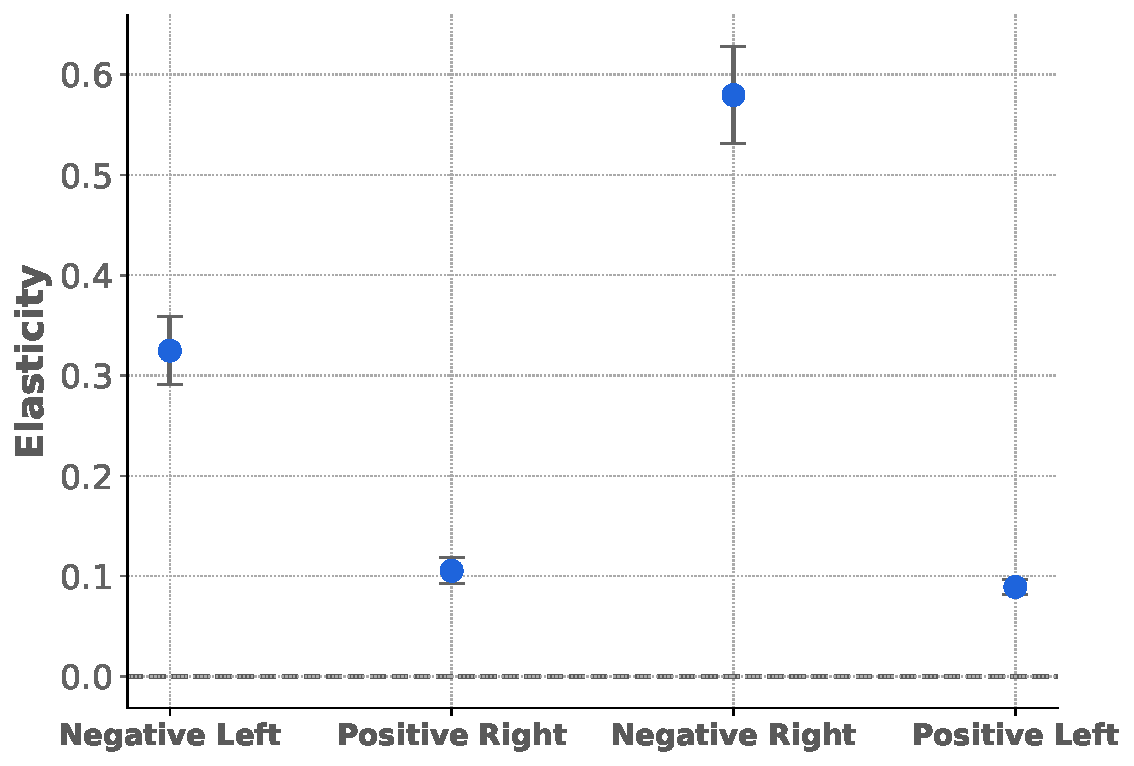
\includegraphics[width=\linewidth]{figures/elasticities_right_pre}
			\label{fig:2figsA}
		\end{minipage}
		
		\vspace{0.5em} % space between figures and note
		
		\captionsetup{justification=justified}
		\caption*{\textit{Note:} \small Each panel shows estimated mean own elasticities for consumer responses  as described in equation \ref{eq:elasticities} for the off-campaign period. Panel (a) reports results for the left-leaning markets, while Panel (b) shows the results for the right-leaning markets. Right markets are defined as regions with proportion of right wing voters above the median. Whiskers represent the $95\%$ confidence intervals of the mean across markets.}
	\end{figure}
	
	
	
	\begin{figure}[ht!]
		\centering
		\caption{Added Variable Plots for Production of Political Content (within day)}
		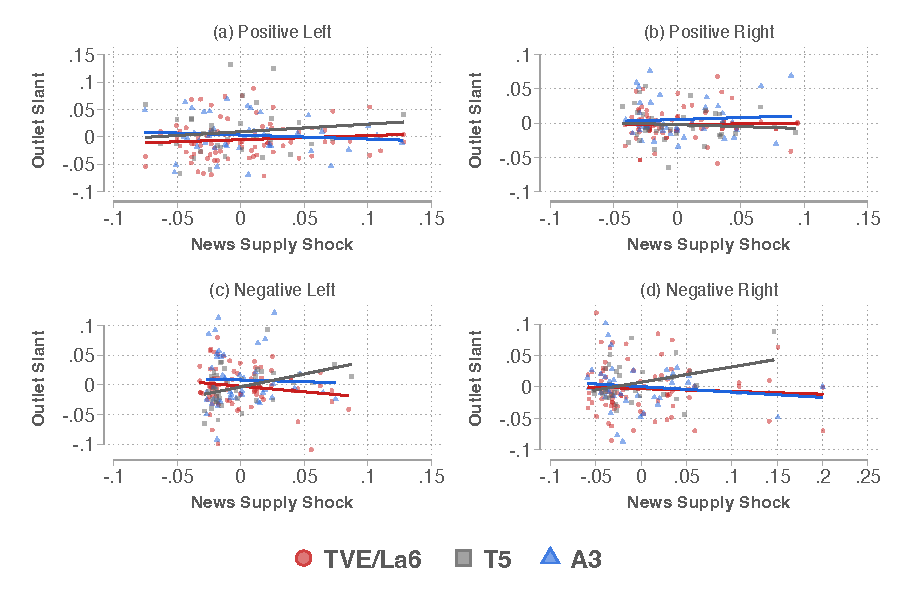
\includegraphics[width=160mm]{figures/fwl_plots_lowess_diff_costs_v2}
		\caption*{\small \textit{Note:} The figure shows the added variable plots from the analogous estimation of equation \ref{eq:first_stage} using within day differences. The x axis represents $\left(\Delta z_d^{party,+},\Delta z_d^{party,-}\right) $ and the y axis the corresponding  $\left(\Delta x_{jd}^{party,+},\Delta x_{jd}^{party,-}\right) $   . Channels are pooled into left (TVE and La Sexta), middle (Telecinco) and right (A3) for visualization purposes.  }
		\label{fig:fwl_diff}
	\end{figure}
	
	
	\begin{comment}
		content...

	\begin{figure}[ht]
		\centering
		\caption{Normalized Ideology Scores by Channel}
		% Panel (a): ChatGPT-based
		\begin{minipage}[t]{0.48\textwidth}
			\centering
			\textit{(a) Demand: Viewers' Elasticities}
			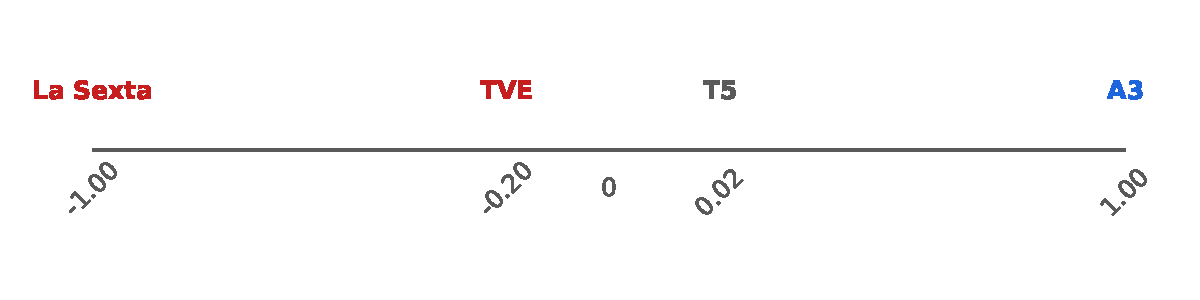
\includegraphics[width=\linewidth]{figures/congress_line_audience_share}
		\end{minipage}
		\hfill
		% Panel (b): CIS-based
		\begin{minipage}[t]{0.48\textwidth}
			\centering
			
			
			\textit{(b) Supply: ChatGPT text classification}
			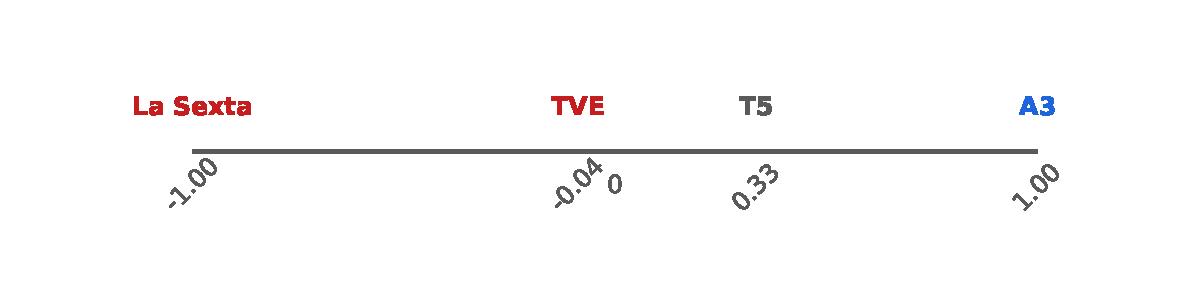
\includegraphics[width=\linewidth]{figures/congress_line_chatgpt_campaign}
			
			
		\end{minipage}
		
		
		\caption*{\small \textit{Notes:} The figure compares normalized left–right audience positions for Spanish television channels. Panel (a) positions channels according to the demand elasticities from the BLP estimation. Panel (b) shows the relative  positions of the slant for the campaign according to the ChatGPT classification. 			Channels are mapped into the $[-1,1]$ scale with the two extreme ones forced into these values to compare across magnitudes.  }
		\label{fig:channel_ideology_lines2}
	\end{figure}
	
		\end{comment}
	
	\begin{figure}[ht!]
		\centering
		\caption{Political and Media Polarization (no-smoothing)}
		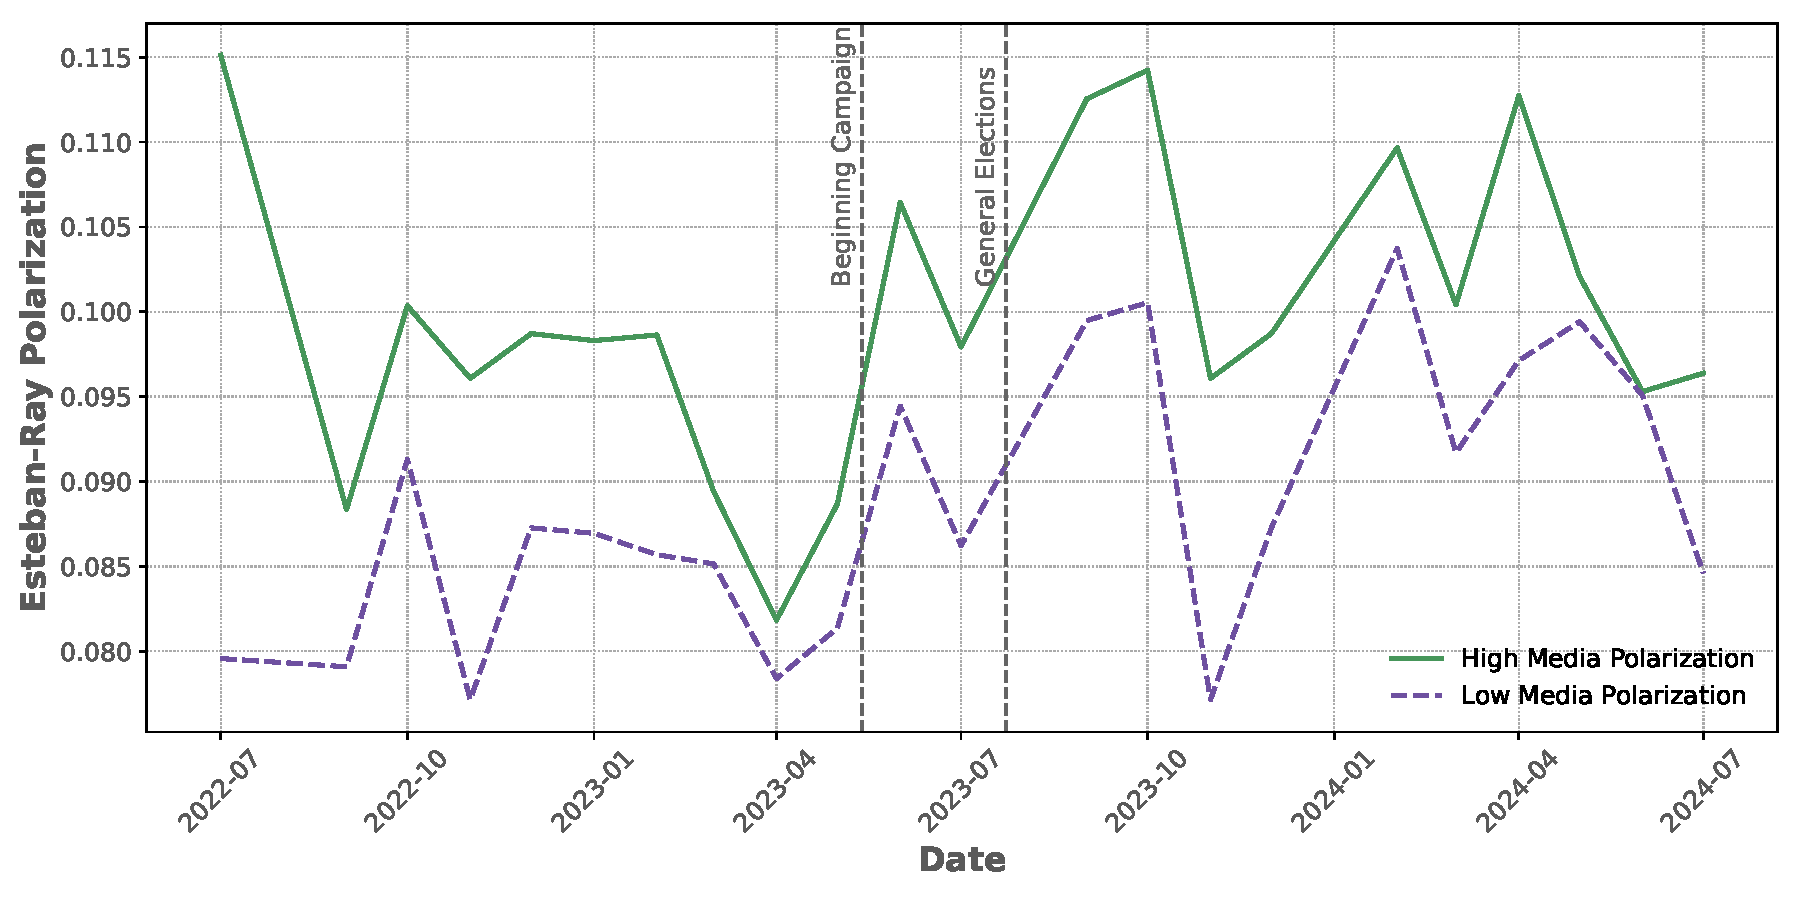
\includegraphics[width=150mm]{figures/er_polarization_stata_group_raw}
		\caption*{\textit{Note:} \small The figure shows the mean Esteban-Ray polarization index  computed as in equation \ref{eq:er}.  Solid (dashed) line represents the regions above (below) the median in terms of their media polarization consumption according to index \ref{eq:mediapol}.   }
		\label{fig:er}
	\end{figure}
	
	
	
	
	\begin{figure}[!htb]
		\centering
		\caption{Change in Positions Factual vs Counterfactual}
		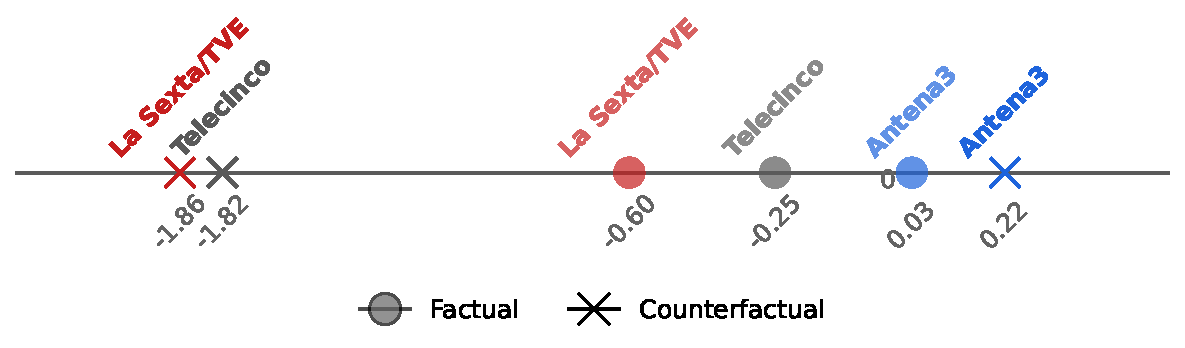
\includegraphics[width=100mm]{figures/congress_line_counter}
		
		\caption*{\small \textit{Note:} The figure shows the relative change in  slant positions  according to the ideological index in Equation \ref{eq:ideo_index} from the factual to the counterfactual during the Campaign period.  }
		\label{fig:change_line_counter}
	\end{figure}
	
	
	
	
	\clearpage

\section{Tables}
	
	
	
	\begin{table}[!htbp]
		\centering
		\caption{Pearson Correlation of Ideology Index  with Agencia EFE}
		\begin{tabular}{lcc}
			\toprule
			\textbf{Channel} & \textbf{Political} & \textbf{Ideology Index} \\
			\midrule
			Antena 3 & 0.666 & 0.364 \\
			T5 & 0.487 & 0.018 \\
			TVE & 0.381 & 0.320 \\
			La Sexta & 0.266 & 0.240 \\
			\bottomrule
		\end{tabular}
		\caption*{\small \textit{Note:} Pearson correlation coefficients ($r$) for the time series of political coverage and the ideology index  in Equation \ref{eq:ideo_index} between each TV channel and Agencia EFE.}
		\label{tab:correlations}
	\end{table}
	
	
	
	\subsection{Descriptive Evidence}
	
	
	
	\begin{table}[!htbp]
		\centering
		\caption{Proportion of Political Content and Sentiment by Channel}
		\begin{tabular}{llcc}
			\toprule
			\textbf{Outlet} & \textbf{Category} & \textbf{Pre-campaign} & \textbf{During campaign} \\
			\midrule
			\midrule
			\multirow{5}{*}{\textbf{A3}}& Negative Left & 0.106 & 0.090 \\
			& Negative Right & 0.043 & 0.066 \\
			& Positive Left & 0.065 & 0.061 \\
			& Positive Right & 0.023 & 0.039 \\
			& Political & 0.277 & 0.387 \\
			\midrule
			\multirow{5}{*}{\textbf{La Sexta}}& Negative Left & 0.041 & 0.032 \\
			& Negative Right & 0.047 & 0.067 \\
			& Positive Left & 0.049 & 0.057 \\
			& Positive Right & 0.013 & 0.012 \\
			& Political & 0.207 & 0.277 \\
			\midrule
			\multirow{5}{*}{\textbf{TVE}}& Negative Left & 0.038 & 0.037 \\
			& Negative Right & 0.045 & 0.046 \\
			& Positive Left & 0.072 & 0.052 \\
			& Positive Right & 0.012 & 0.021 \\
			& Political & 0.175 & 0.212 \\
			\midrule
			\multirow{5}{*}{\textbf{T5}}& Negative Left & 0.043 & 0.039 \\
			& Negative Right & 0.025 & 0.044 \\
			& Positive Left & 0.047 & 0.046 \\
			& Positive Right & 0.012 & 0.026 \\
			& Political & 0.111 & 0.183 \\
			\bottomrule
				\multirow{5}{*}{\textbf{Agencia EFE}} & Negative Left & 0.076 & 0.073 \\
			& Negative Right & 0.058 & 0.094\\
			& Positive Left & 0.138 & 0.145 \\
			& Positive Right & 0.043 & 0.099\\
			& Political & 0.438 & 0.515 \\
			\bottomrule
			
		\end{tabular}
		\caption*{\small \textit{Note:} The table shows the proportion of political minutes and the breakdown by tone/party for each channel, off- and during campaign. For Agencia EFE it shows the proportion of stories of each category. }
		\label{tab:political_sentiment_types}
	\end{table}
	
	
	
	
	\begin{table}[!htbp]
		\centering
		\caption{Proportion of Positive/Negative Minutes by Channel}
		\begin{tabular}{llcc}
			\toprule
			\textbf{Outlet} & \textbf{Category} & \textbf{Pre-campaign} & \textbf{During campaign} \\
			\midrule
			\midrule
			\multirow{4}{*}{\textbf{A3}} & Positive Left & 0.065 & 0.061 \\
			& Positive Right & 0.023 & 0.039 \\
			& Negative Left & 0.106 & 0.090 \\
			& Negative Right & 0.043 & 0.066 \\
			\midrule
			\multirow{4}{*}{\textbf{La Sexta}} & Positive Left & 0.049 & 0.057 \\
			& Positive Right & 0.013 & 0.012 \\
			& Negative Left & 0.041 & 0.032 \\
			& Negative Right & 0.047 & 0.067 \\
			\midrule
			\multirow{4}{*}{\textbf{T5}} & Positive Left & 0.047 & 0.046 \\
			& Positive Right & 0.012 & 0.026 \\
			& Negative Left & 0.043 & 0.039 \\
			& Negative Right & 0.025 & 0.044 \\
			\midrule
			\multirow{4}{*}{\textbf{TVE}} & Positive Left & 0.072 & 0.052 \\
			& Positive Right & 0.012 & 0.021 \\
			& Negative Left & 0.038 & 0.037 \\
			& Negative Right & 0.045 & 0.046 \\
			\midrule
			\bottomrule
		\end{tabular}
		\caption*{\small \textit{Note:} The table shows the proportion of positive and negative minutes for each channel, off- and during campaign.}
		\label{tab:positive_negative_minutes}
	\end{table}
	
	
	
	\subsection{Additional Results}
	

	
	
	
	
	
	\begin{comment}
		
		
		
		\begin{table}[!htb]
			\centering
			
			\caption{Effect of Mentions on Tone toward Party Leaders}
			\label{tab:images2}
			\small
			\setlength{\tabcolsep}{4pt}
			\renewcommand{\arraystretch}{1.0}
			\begin{tabular}{lcccc}
				\toprule
				& \multicolumn{4}{c}{\textit{Outlet Slant} (\(x\))} \\
				\cmidrule(lr){2-5}
				& (1) & (2) & (3) & (4) \\
				\midrule
				
				\multicolumn{5}{l}{\textbf{Feijóo (PP)}}\\
				Text Mentions     &  -1.956         &  -3.038         &   0.364         &   -1.342        \\
				&  (2.063)        &  (2.134)        &  (2.391)        &  (2.584)        \\
				Image Appearances &  -0.065         &   0.003         &  -0.275         &  -0.189         \\
				&  (0.147)        &  (0.151)        &  (0.179)        &  (0.189)        \\
				\addlinespace
				\hline
				\multicolumn{5}{l}{\textbf{Abascal (VOX)}}\\
				Text Mentions     & -42.813\sym{***}& -44.024\sym{***}& -46.659\sym{***}& -49.989\sym{***}\\
				&  (7.855)        &  (7.832)        &  (9.609)        &  (9.471)        \\
				Image Appearances &   0.963\sym{**} &   0.933\sym{**} &   0.565         &   0.437         \\
				&  (0.470)        &  (0.470)        &  (0.600)        &  (0.595)        \\
				\addlinespace
				\hline
				\multicolumn{5}{l}{\textbf{Sánchez (PSOE)}}\\
				Text Mentions     &   4.131         &  11.634\sym{*}  &   2.648         &  13.515\sym{*}  \\
				&  (6.020)        &  (6.992)        &  (6.494)        &  (7.909)        \\
				Image Appearances &   0.023         &  -0.045         &   0.033         &   0.032         \\
				&  (0.239)        &  (0.244)        &  (0.356)        &  (0.377)        \\
				\addlinespace
				\hline
				\multicolumn{5}{l}{\textbf{Díaz (UP)}}\\
				Text Mentions     &  -0.576         &   1.276         &  -0.714         &   3.365         \\
				&  (3.158)        &  (3.280)        &  (4.080)        &  (4.405)        \\
				Image Appearances &   0.473\sym{**} &   0.485\sym{**} &   0.290         &   0.321         \\
				&  (0.197)        &  (0.206)        &  (0.232)        &  (0.247)        \\
				\midrule
				Channel FE        & No              & Yes             & No              & Yes             \\
				Date FE           & No              & No              & Yes             & Yes             \\
				\midrule
				Observations      & 231             & 231             & 231             & 227             \\
				\bottomrule
			\end{tabular}
			
			\vspace{0.5em}
			\begin{flushleft}
				\scriptsize\emph{Note:} Robust standard errors in parentheses;\quad 
				\sym{*} \(p<0.05\), \sym{**} \(p<0.01\), \sym{***} \(p<0.001\).  
				Each block shows coefficients from regressing net tone on text mentions and image appearances of the party leader.
			\end{flushleft}
		\end{table}
		
		
This is the table when i run the regression separatedly without both controls on the same regression ( multicollinearity). 

	\begin{table}[!htb]
		\centering
		\caption{Effect of Mentions on Tone toward Party Leaders}
		\label{tab:images}
		\small
		\setlength{\tabcolsep}{4pt}
		\renewcommand{\arraystretch}{1.0}
		\begin{tabular}{lcccc}
			\toprule
			& \multicolumn{4}{c}{\textit{Outlet Slant} (\(x\))} \\
			\cmidrule(lr){2-5}
			& (1) No FE & (2) Channel FE & (3) Date FE & (4) Both FE \\
			\midrule
			
			\multicolumn{5}{l}{\textbf{Feijóo (PP)}}\\
			Text Mentions     &  -2.583         &  -3.145\sym{*}  &  -1.181         &  -2.112         \\
			&  (1.601)        &  (1.693)        &  (1.988)        &  (2.231)        \\
			Image Appearances &  -0.141         &  -0.109         &  -0.263         &  -0.222         \\
			&  (0.124)        &  (0.129)        &  (0.161)        &  (0.178)        \\
			\addlinespace
			\hline
			
			\multicolumn{5}{l}{\textbf{Abascal (Vox)}}\\
			Text Mentions     & -35.693\sym{***}& -37.210\sym{***}& -43.668\sym{***}& -46.976\sym{***}\\
			&  (6.742)        &  (6.725)        &  (8.891)        &  (8.843)        \\
			Image Appearances &  -0.093         &  -0.149         &  -0.039         &  -0.173         \\
			&  (0.455)        &  (0.457)        &  (0.625)        &  (0.630)        \\
			\addlinespace
			\hline
			
			\multicolumn{5}{l}{\textbf{Sánchez (PSOE)}}\\
			Text Mentions     &   4.359         &  11.306\sym{*}  &   1.957         &  12.359\sym{*}  \\
			&  (5.139)        &  (5.975)        &  (5.460)        &  (6.879)        \\
			Image Appearances &   0.096         &   0.135         &   0.088         &   0.236         \\
			&  (0.214)        &  (0.220)        &  (0.329)        &  (0.360)        \\
			\addlinespace
			\hline
			
			\multicolumn{5}{l}{\textbf{Díaz (UP)}}\\
			Text Mentions     &   2.739         &   4.778\sym{*}  &   0.993         &   5.037         \\
			&  (2.637)        &  (2.730)        &  (3.678)        &  (3.961)        \\
			Image Appearances &   0.456\sym{***}&   0.524\sym{***}&   0.277         &   0.381         \\
			&  (0.172)        &  (0.179)        &  (0.217)        &  (0.234)        \\
			\midrule
			Channel FE        & No              & Yes             & No              & Yes             \\
			Date FE           & No              & No              & Yes             & Yes             \\
			\midrule
			Observations      & 231             & 231             & 231             & 227             \\
			\bottomrule
		\end{tabular}
		
		\vspace{0.5em}
		\begin{flushleft}
			\scriptsize\emph{Note:} Robust standard errors in parentheses;\quad
			\sym{*} \(p<0.05\), \sym{**} \(p<0.01\), \sym{***} \(p<0.001\).  
			Each block reports the text‐only and image‐only coefficients under four FE specifications; Observations are from the image‐only models.
		\end{flushleft}
	\end{table}
	
		\end{comment}
	
	
	\begin{comment}
		content...

	
	
	\begin{table}[!htb]\centering
		\def\sym#1{\ifmmode^{#1}\else\(^{#1}\)\fi}
		\caption{Effect of Mentions on Tone toward Feijóo}
		\begin{tabular}{l*{4}{c}}
			\hline\hline
				\multicolumn{1}{c}{} & \multicolumn{4}{c}{\textit{Outlet Slant $(x)$}} \\ 
			\cline{2-5}
			&\multicolumn{1}{c}{(1)}         &\multicolumn{1}{c}{(2)}         &\multicolumn{1}{c}{(3)}         &\multicolumn{1}{c}{(4)}         \\
			\hline
			Text Mentions   &  -25.763         &  -51.515         &   42.517         &    6.957         \\
			& (50.044)         & (51.028)         & (61.383)         & (64.934)         \\
			Image Appearances  &   -4.373         &   -2.024         &  -12.421\sym{**} &   -9.379\sym{*}  \\
			&  (3.785)         &  (3.852)         &  (4.815)         &  (5.112)         \\
			constant          &   -0.088         &   -0.093         &   -0.049         &   -0.053         \\
			&  (0.076)         &  (0.077)         &  (0.093)         &  (0.101)         \\
			Channel FE      &       No         &      Yes         &       No         &      Yes         \\
			Date FE         &       No         &       No         &      Yes         &      Yes         \\
			\hline
			Observations    &      238         &      238         &      234         &      234         \\
			\hline\hline
		\end{tabular}
		\label{tab:feijoo_images}
		\vspace{0.5em}
		\caption*{\scriptsize\emph{Note:} Robust standard errors in parentheses. The table shows the estimated coefficients for a regression of net tone on the People's Party calculated as in \ref{eq:controls}, on the proportion of image appearances and text mentions of its party leader, Feijoo. Results are for a random sample of 67 days. }
	\end{table}
	
	
	\begin{table}[!htb]\centering
		\def\sym#1{\ifmmode^{#1}\else\(^{#1}\)\fi}
		\caption{Effect of Mentions on Tone toward Abascal}
		\begin{tabular}{l*{4}{c}}
			\hline\hline
				\multicolumn{1}{c}{} & \multicolumn{4}{c}{\textit{Outlet Slant $(x)$}} \\ 
			\cline{2-5}
			&\multicolumn{1}{c}{(1)}         &\multicolumn{1}{c}{(2)}         &\multicolumn{1}{c}{(3)}         &\multicolumn{1}{c}{(4)}         \\
			\hline
			Text Mentions   & -506.623\sym{***}& -534.081\sym{***}& -539.867\sym{***}& -609.038\sym{***}\\
			&(148.973)         &(147.122)         &(161.979)         &(156.866)         \\
			Image Appearances  &   18.013\sym{**} &   15.994\sym{*}  &   22.023\sym{**} &   17.193\sym{*}  \\
			&  (9.077)         &  (8.996)         & (10.119)         &  (9.898)         \\
			constant          &   -0.122\sym{**} &   -0.109\sym{*}  &   -0.130\sym{**} &   -0.099\sym{*}  \\
			&  (0.057)         &  (0.056)         &  (0.057)         &  (0.056)         \\
			Channel FE      &       No         &      Yes         &       No         &      Yes         \\
			Date FE         &       No         &       No         &      Yes         &      Yes         \\
			\hline
			Observations    &      238         &      238         &      234         &      234         \\
			\hline\hline
		\end{tabular}
		\label{tab:abascal_images}
		\vspace{0.5em}
		\caption*{\scriptsize\emph{Note:} Robust standard errors in parentheses. The table shows the estimated coefficients for a regression of net tone on VOX calculated as in \ref{eq:controls}, on the proportion of image appearances and text mentions of its party leader, Abascal. Results are for a random sample of 67 days. }
	\end{table}
	
	
	\begin{table}[!htb]\centering
		\def\sym#1{\ifmmode^{#1}\else\(^{#1}\)\fi}
		\caption{Effect of Mentions on Tone toward Sánchez}
		\begin{tabular}{l*{4}{c}}
			\hline\hline
				\multicolumn{1}{c}{} & \multicolumn{4}{c}{\textit{Outlet Slant $(x)$}} \\ 
			\cline{2-5}
			&\multicolumn{1}{c}{(1)}         &\multicolumn{1}{c}{(2)}         &\multicolumn{1}{c}{(3)}         &\multicolumn{1}{c}{(4)}         \\
			\hline
			Text Mentions   &   61.471         &  196.424         &   27.282         &  193.827         \\
			&(106.565)         &(123.145)         &(119.969)         &(145.161)         \\
			Image Appearances  &   -2.352         &   -4.286         &   -7.639         &  -10.754         \\
			&  (4.253)         &  (4.331)         &  (6.583)         &  (6.971)         \\
			constant          &    0.054         &    0.014         &    0.120         &    0.077         \\
			&  (0.063)         &  (0.067)         &  (0.075)         &  (0.085)         \\
			Channel FE      &       No         &      Yes         &       No         &      Yes         \\
			Date FE         &       No         &       No         &      Yes         &      Yes         \\
			\hline
			Observations    &      238         &      238         &      234         &      234         \\
			\hline\hline
		\end{tabular}
		\label{tab:sanchez_images}
		\vspace{0.5em}
		\caption*{\scriptsize\emph{Note:} Robust standard errors in parentheses. The table shows the estimated coefficients for a regression of net tone on PSOE calculated as in \ref{eq:controls}, on the proportion of image appearances and text mentions of its party leader, Sánchez. Results are for a random sample of 67 days. }
	\end{table}
	
	
	\begin{table}[!htb]\centering
		\def\sym#1{\ifmmode^{#1}\else\(^{#1}\)\fi}
		\caption{Effect of Mentions on Tone toward Díaz}
		\begin{tabular}{l*{4}{c}}
			\hline\hline
				\multicolumn{1}{c}{} & \multicolumn{4}{c}{\textit{Outlet Slant $(x)$}} \\ 
			\cline{2-5}
			&\multicolumn{1}{c}{(1)}         &\multicolumn{1}{c}{(2)}         &\multicolumn{1}{c}{(3)}         &\multicolumn{1}{c}{(4)}         \\
			\hline
			Text Mentions   &  -11.990         &   21.235         &  -78.607         &  -19.353         \\
			& (67.519)         & (69.918)         & (91.794)         & (99.632)         \\
			Image Appearances  &    0.019         &   -0.072         &   -0.861         &   -1.032\sym{*}  \\
			&  (0.512)         &  (0.517)         &  (0.595)         &  (0.603)         \\
			constant          &    0.064         &    0.051         &    0.103\sym{**} &    0.080         \\
			&  (0.044)         &  (0.045)         &  (0.051)         &  (0.054)         \\
			Channel FE      &       No         &      Yes         &       No         &      Yes         \\
			Date FE         &       No         &       No         &      Yes         &      Yes         \\
			\hline
			Observations    &      238         &      238         &      234         &      234         \\
			\hline\hline
		\end{tabular}
		\label{tab:diaz_images}
		\vspace{0.5em}
		\caption*{\scriptsize\emph{Note:} Robust standard errors in parentheses. The table shows the estimated coefficients for a regression of net tone on UP calculated as in \ref{eq:controls}, on the proportion of image appearances and text mentions of its party leader, Díaz. Results are for a random sample of 67 days. }
	\end{table}
	
	

	
	\begin{table}[htbp]
		\centering
		\scriptsize
		\setlength{\tabcolsep}{4pt}
		\renewcommand{\arraystretch}{0.9}
		\caption{First Stage Regressions}
		\label{tab:first_stage}
		\begin{tabular}{lcccc}
		\hline
		% span columns 2–5 (the four slant columns)
		\multicolumn{1}{c}{} & \multicolumn{4}{c}{\textit{Outlet Slant $(x)$}} \\ 
		\cline{2-5}
		& \textbf{(1) Positive Right}
		& \textbf{(2) Negative Right}
		& \textbf{(3) Positive Left}
		& \textbf{(4) Negative Left} \\
		\hline
			
			% Single grouping header
			\multicolumn{5}{l}{\textit{News‐Shock $(z)$}}\\
			\hline
			
			% Now only the short block names
			\multicolumn{5}{l}{\textbf{Positive Right}}\\
			\hline
			TVE            &  0.00342         & -0.00456         & -0.0498         & -0.0916         \\
			&  (0.08)          & (-0.07)          & (-0.71)         & (-1.30)         \\
			A3             &  0.207\sym{***}  & -0.139           & -0.0615         & -0.113          \\
			&  (4.62)          & (-1.89)          & (-0.81)         & (-1.47)         \\
			T5             & -0.0372          & -0.0746          & -0.0943         & -0.166\sym{*}   \\
			& (-0.88)          & (-1.08)          & (-1.31)         & (-2.28)         \\
			La Sexta       &  0.0334          & -0.0129          &  0.0290         & -0.0256         \\
			&  (0.73)          & (-0.17)          &  (0.37)         & (-0.33)         \\
			\hline
			
			\multicolumn{5}{l}{\textbf{Negative Right}}\\
			\hline
			TVE            & -0.0296          &  0.00590         & -0.0707         &  0.0738         \\
			& (-0.74)          &  (0.09)          & (-1.04)         &  (1.08)         \\
			A3             & -0.0333          &  0.0929          & -0.0104         & -0.0440         \\
			& (-0.79)          &  (1.34)          & (-0.14)         & (-0.61)         \\
			T5             & -0.0585          &  0.131           &  0.0327         & -0.0166         \\
			& (-1.05)          &  (1.44)          &  (0.35)         & (-0.17)         \\
			La Sexta       & -0.0185          &  0.143\sym{*}    & -0.0399         & -0.123          \\
			& (-0.42)          &  (1.97)          & (-0.53)         & (-1.63)         \\
			\hline
			
			\multicolumn{5}{l}{\textbf{Positive Left}}\\
			\hline
			TVE            &  0.0261         &  0.0634         &  0.200\sym{**}  & -0.0511         \\
			&  (0.68)         &  (1.01)         &  (3.07)         & (-0.78)         \\
			A3             &  0.00911        & -0.0626         &  0.0154         & -0.0845         \\
			&  (0.22)         & (-0.92)         &  (0.22)         & (-1.19)         \\
			T5             & -0.0712         & -0.159          & -0.00405        & -0.0572         \\
			& (-1.43)         & (-1.95)         & (-0.05)         & (-0.67)         \\
			La Sexta       &  0.00655        & -0.0906         & -0.00875        &  0.0718         \\
			&  (0.16)         & (-1.33)         & (-0.12)         &  (1.01)         \\
			\hline
			
			\multicolumn{5}{l}{\textbf{Negative Left}}\\
			\hline
			TVE            &  0.0144         & -0.0603         & -0.176\sym{*}   &  0.149          \\
			&  (0.32)         & (-0.81)         & (-2.26)         &  (1.90)         \\
			A3             &  0.0446         & -0.133          & -0.173\sym{*}   &  0.184\sym{*}   \\
			&  (0.93)         & (-1.69)         & (-2.11)         &  (2.23)         \\
			T5             & -0.141\sym{**}  &  0.0136         & -0.00461        & -0.0569         \\
			& (-2.66)         &  (0.16)         & (-0.05)         & (-0.63)         \\
			La Sexta       &  0.0262         & -0.141          & -0.139          &  0.111          \\
			&  (0.53)         & (-1.73)         & (-1.65)         &  (1.31)         \\
			\hline\hline
		\end{tabular}
		\caption*{\scriptsize\emph{Note:} Robust standard errors in parentheses; \sym{*} $p<0.05$, \sym{**} $p<0.01$, \sym{***} $p<0.001$. Total observations: $N=687$.}
	\end{table}
	
			\end{comment}
	
	\begin{table}[htbp]
		\centering
		\scriptsize
		\setlength{\tabcolsep}{4pt}
		\renewcommand{\arraystretch}{0.9}
		\caption{First Stage Regressions}
		\label{tab:first_stage}
		\begin{tabular}{lcccc}
			\hline
			\multicolumn{1}{c}{} & \multicolumn{4}{c}{\textit{Outlet Slant $(x)$}} \\ 
			\cline{2-5}
			& \textbf{(1) Positive Right}
			& \textbf{(2) Negative Right}
			& \textbf{(3) Positive Left}
			& \textbf{(4) Negative Left} \\
			\hline
			
			\multicolumn{5}{l}{\textit{News‐Shock $(z)$}}\\
			\hline
			
			\multicolumn{5}{l}{\textbf{Positive Right}}\\
			\hline
			TVE            &  0.00342         & -0.00456         & -0.0498         & -0.0916         \\
			&  (0.08)          & (-0.07)          & (-0.71)         & (-1.30)         \\
			A3             &  0.207\sym{***}  & -0.139           & -0.0615         & -0.113          \\
			&  (4.62)          & (-1.89)          & (-0.81)         & (-1.47)         \\
			T5             & -0.0372          & -0.0746          & -0.0943         & -0.166\sym{*}   \\
			& (-0.88)          & (-1.08)          & (-1.31)         & (-2.28)         \\
			La Sexta       &  0.0334          & -0.0129          &  0.0290         & -0.0256         \\
			&  (0.73)          & (-0.17)          &  (0.37)         & (-0.33)         \\
			\hline
			
			\multicolumn{5}{l}{\textbf{Negative Right}}\\
			\hline
			TVE            & -0.0296          &  0.00590         & -0.0707         &  0.0738         \\
			& (-0.74)          &  (0.09)          & (-1.04)         &  (1.08)         \\
			A3             & -0.0333          &  0.0929          & -0.0104         & -0.0440         \\
			& (-0.79)          &  (1.34)          & (-0.14)         & (-0.61)         \\
			T5             & -0.0585          &  0.131           &  0.0327         & -0.0166         \\
			& (-1.05)          &  (1.44)          &  (0.35)         & (-0.17)         \\
			La Sexta       & -0.0185          &  0.143\sym{*}    & -0.0399         & -0.123          \\
			& (-0.42)          &  (1.97)          & (-0.53)         & (-1.63)         \\
			\hline
			
			\multicolumn{5}{l}{\textbf{Positive Left}}\\
			\hline
			TVE            &  0.0261         &  0.0634         &  0.200\sym{**}  & -0.0511         \\
			&  (0.68)         &  (1.01)         &  (3.07)         & (-0.78)         \\
			A3             &  0.00911        & -0.0626         &  0.0154         & -0.0845         \\
			&  (0.22)         & (-0.92)         &  (0.22)         & (-1.19)         \\
			T5             & -0.0712         & -0.159          & -0.00405        & -0.0572         \\
			& (-1.43)         & (-1.95)         & (-0.05)         & (-0.67)         \\
			La Sexta       &  0.00655        & -0.0906         & -0.00875        &  0.0718         \\
			&  (0.16)         & (-1.33)         & (-0.12)         &  (1.01)         \\
			\hline
			
			\multicolumn{5}{l}{\textbf{Negative Left}}\\
			\hline
			TVE            &  0.0144         & -0.0603         & -0.176\sym{*}   &  0.149          \\
			&  (0.32)         & (-0.81)         & (-2.26)         &  (1.90)         \\
			A3             &  0.0446         & -0.133          & -0.173\sym{*}   &  0.184\sym{*}   \\
			&  (0.93)         & (-1.69)         & (-2.11)         &  (2.23)         \\
			T5             & -0.141\sym{**}  &  0.0136         & -0.00461        & -0.0569         \\
			& (-2.66)         &  (0.16)         & (-0.05)         & (-0.63)         \\
			La Sexta       &  0.0262         & -0.141          & -0.139          &  0.111          \\
			&  (0.53)         & (-1.73)         & (-1.65)         &  (1.31)         \\
			\hline
			
			\multicolumn{5}{l}{\textbf{Political}}\\
			\hline
			TVE            &  0.0167         &  0.0680\sym{*}   &  0.0828\sym{*}  &  0.0494         \\
			&  (0.82)         &  (2.03)         &  (2.38)         &  (1.41)         \\
			A3             &  0.0187         &  0.145\sym{***}  &  0.137\sym{***} &  0.175\sym{***} \\
			&  (0.84)         &  (3.98)         &  (3.62)         &  (4.59)         \\
			T5             &  0.0975\sym{***}&  0.0981\sym{*}   &  0.0837 &  0.125\sym{**}  \\
			&  (3.69)         &  (2.26)         &  (1.86)         &  (2.77)         \\
			La Sexta       &  0.0145         &  0.132\sym{***}  &  0.123\sym{**}  &  0.0393         \\
			&  (0.63)         &  (3.47)         &  (3.12)         &  (0.99)         \\
			\hline\hline
		\end{tabular}
		\caption*{\scriptsize\emph{Note:} Robust standard errors in parentheses; 
			 $p<0.1$, \sym{*} $p<0.05$, \sym{**} $p<0.01$, \sym{***} $p<0.001$. 
			Total observations: $N=687$.}
	\end{table}
	
	
	
	
	
	
	
	
	
	
\begin{comment}


\begin{table}[htbp]
	\centering
	\scriptsize
	\setlength{\tabcolsep}{4pt}
	\renewcommand{\arraystretch}{0.9}
	\def\sym#1{\ifmmode^{#1}\else\(^{#1}\)\fi}
	\caption{First Stage Regressions}
	\label{tab:first_stage}
	\begin{tabular}{lcccc}
		\hline\hline
		& \multicolumn{1}{c}{(1) Positive Right}
		& \multicolumn{1}{c}{(2) Negative Right}
		& \multicolumn{1}{c}{(3) Positive Left}
		& \multicolumn{1}{c}{(4) Negative Left} \\
		\hline
		\multicolumn{5}{l}{\textbf{Positive Right (All)}}\\
				\hline
		TVE            &  0.00342         & -0.00456         & -0.0498         & -0.0916         \\
		&  (0.08)          & (-0.07)          & (-0.71)         & (-1.30)         \\
		A3             &  0.207\sym{***}  & -0.139           & -0.0615         & -0.113          \\
		&  (4.62)          & (-1.89)          & (-0.81)         & (-1.47)         \\
		T5             & -0.0372          & -0.0746          & -0.0943         & -0.166\sym{*}   \\
		& (-0.88)          & (-1.08)          & (-1.31)         & (-2.28)         \\
		La Sexta       &  0.0334          & -0.0129          &  0.0290         & -0.0256         \\
		&  (0.73)          & (-0.17)          &  (0.37)         & (-0.33)         \\
		\hline
		\multicolumn{5}{l}{\textbf{Negative Right (All)}}\\
				\hline
		TVE            & -0.0296          &  0.00590         & -0.0707         &  0.0738         \\
		& (-0.74)          &  (0.09)          & (-1.04)         &  (1.08)         \\
		A3             & -0.0333          &  0.0929          & -0.0104         & -0.0440         \\
		& (-0.79)          &  (1.34)          & (-0.14)         & (-0.61)         \\
		T5             & -0.0585          &  0.131           &  0.0327         & -0.0166         \\
		& (-1.05)          &  (1.44)          &  (0.35)         & (-0.17)         \\
		La Sexta       & -0.0185          &  0.143\sym{*}    & -0.0399         & -0.123          \\
		& (-0.42)          &  (1.97)          & (-0.53)         & (-1.63)         \\
		\hline
		\multicolumn{5}{l}{\textbf{Positive Left (All)}}\\
				\hline
		TVE            &  0.0261         &  0.0634         &  0.200\sym{**}  & -0.0511         \\
		&  (0.68)         &  (1.01)         &  (3.07)         & (-0.78)         \\
		A3             &  0.00911        & -0.0626         &  0.0154         & -0.0845         \\
		&  (0.22)         & (-0.92)         &  (0.22)         & (-1.19)         \\
		T5             & -0.0712         & -0.159          & -0.00405        & -0.0572         \\
		& (-1.43)         & (-1.95)         & (-0.05)         & (-0.67)         \\
		La Sexta       &  0.00655        & -0.0906         & -0.00875        &  0.0718         \\
		&  (0.16)         & (-1.33)         & (-0.12)         &  (1.01)         \\
		\hline
		\multicolumn{5}{l}{\textbf{Negative Left (All)}}\\
				\hline
		TVE            &  0.0144         & -0.0603         & -0.176\sym{*}   &  0.149          \\
		&  (0.32)         & (-0.81)         & (-2.26)         &  (1.90)         \\
		A3             &  0.0446         & -0.133          & -0.173\sym{*}   &  0.184\sym{*}   \\
		&  (0.93)         & (-1.69)         & (-2.11)         &  (2.23)         \\
		T5             & -0.141\sym{**}  &  0.0136         & -0.00461        & -0.0569         \\
		& (-2.66)         &  (0.16)         & (-0.05)         & (-0.63)         \\
		La Sexta       &  0.0262         & -0.141          & -0.139          &  0.111          \\
		&  (0.53)         & (-1.73)         & (-1.65)         &  (1.31)         \\
		\hline
		\multicolumn{5}{l}{\textbf{Political (All)}}\\
				\hline
		TVE            &  0.0167         &  0.0680\sym{*}  &  0.0828\sym{*}  &  0.0494         \\
		&  (0.82)         &  (2.03)         &  (2.38)         &  (1.41)         \\
		A3             &  0.0187         &  0.145\sym{***}&  0.137\sym{***}&  0.175\sym{***}\\
		&  (0.84)         &  (3.98)         &  (3.62)         &  (4.59)         \\
		T5             &  0.0975\sym{***}&  0.0981\sym{*}  &  0.0837         &  0.125\sym{**}  \\
		&  (3.69)         &  (2.26)         &  (1.86)         &  (2.77)         \\
		La Sexta       &  0.0145         &  0.132\sym{***}&  0.123\sym{**} &  0.0393         \\
		&  (0.63)         &  (3.47)         &  (3.12)         &  (0.99)         \\
		\hline\hline
	\end{tabular}
	
	\caption*{\scriptsize\emph{Note:} Robust standard errors in  parentheses;\quad \sym{*} $p<0.05$, \sym{**} $p<0.01$, \sym{***} $p<0.001$. The table shows the results of the first stage regressions in equation \ref{eq:first_stage}. The total number of observations is $N=687$ }
	

\end{table}

\end{comment}
	
	
	
	
	
	\begin{table}[!htb]
			\caption{Logit Estimation Results with Standard Errors}
		\label{tab:logit}
		\centering
		\begin{threeparttable}
			\begin{tabular}{lccc}
				\hline
				\textbf{Coefficient} & \textbf{Parameter} & \textbf{Estimate} & \textbf{Std.\ Error} \\
				\hline
				\hline
				\multicolumn{4}{c}{\textbf{Pre-campaign}} \\
				\hline
				Positive Left & $\beta^{L+}$ & -17.62 & (14.344) \\
				Positive Right & $\beta^{R+}$ & -41.16** & (18.718) \\
				Negative Left & $\beta^{L-}$ & 27.24 & (20.268) \\
				Negative Right & $\beta^{R-}$ & 66.04* & (34.668) \\
				Political & $\beta^{political}$ & 14.28* & (7.465) \\
				Weather & $\gamma$ & 0.01 & (0.655) \\
				Positive Left $\times$ Right-Mean & $\phi^{L+}$ & 47.67 & (36.262) \\
				Positive Right $\times$ Right-Mean & $\phi^{R+}$ & 111.13** & (50.798) \\
				Negative Left $\times$ Right-Mean & $\phi^{L-}$ & -81.40 & (51.195) \\
				Negative Right $\times$ Right-Mean & $\phi^{R-}$ & -151.24* & (89.249) \\
				Political $\times$ Right-Mean & $\phi^{political}$ & -30.80 & (18.952) \\
				\hline
				\hline
				\multicolumn{4}{c}{\textbf{Campaign}} \\
				\hline
				Positive Left & $\beta^{L+}$ & 222.18** & (110.419) \\
				Positive Right & $\beta^{R+}$ & -177.76** & (88.006) \\
				Negative Left & $\beta^{L-}$ & -153.39** & (76.074) \\
				Negative Right & $\beta^{R-}$ & 147.85** & (69.428) \\
				Political & $\beta^{political}$ & -10.37** & (5.107) \\
				Weather & $\gamma$ & 0.80*** & (0.287) \\
				Positive Left $\times$ Right-Mean & $\phi^{L+}$ & -619.77** & (303.679) \\
				Positive Right $\times$ Right-Mean & $\phi^{R+}$ & 461.19* & (242.882) \\
				Negative Left $\times$ Right-Mean & $\phi^{L-}$ & 398.26* & (211.132) \\
				Negative Right $\times$ Right-Mean & $\phi^{R-}$ & -413.87** & (187.584) \\
				Political $\times$ Right-Mean & $\phi^{political}$ & 28.91** & (14.181) \\
				\hline
			\end{tabular}

				\begin{tablenotes}
				\small
				\item \footnotesize{The table shows the results of the logit estimation of model \ref{eq:logit}. The estimations are divided into the off-campaign and campaign period. Both day-of-the-week and outlet fixed effects are included. Standard errors are clustered at the region level. The total number of observations are $N_{campaign}=2307$ and  $N_{pre\_campaign}=6604$.}
			\end{tablenotes}
		\end{threeparttable}
	\end{table}
	
	\begin{comment}
		content...

	
\begin{table}[!htb]
	\centering
	\caption{Top 5 Topics by Party-Tone Category on Agencia EFE after BERTopic. }
	\begin{tabular}{|l|c|}
		\hline
				\multicolumn{1}{|c|}{\textbf{Topic Words}}& \textbf{Count} \\
		\hline
		\hline
		\multicolumn{2}{|c|}{\textbf{Positive Right}} \\
		\hline
		vox, motion, abascal, censure, pp, tamames, santiago, garriga, parties, party & 312 \\
		feijóo, núñez, alberto, pp, leader, gamarra, parties, party, general, cuca & 113 \\
		guardiola, extremadura, mérida, maría, vara, extremeño, council, assembly, candidate & 68 \\
		mazón, valencian, president, corts, valencian, valencians, government, carlos & 64 \\
		electoral, elections, general, jec, board, campaign, 28m, 23j, vote & 63 \\
		\hline
		\multicolumn{2}{|c|}{\textbf{Negative Right}} \\
		\hline
		vox, motion, abascal, censure, pp, tamames, santiago, garriga, parties, party & 369 \\
		abortion, castilla, healthcare, anti-abortion,pregnancy, abortions, law, mañueco & 112 \\
		code, criminal, sedition, embezzlement, reform, crime, penalties, amendments & 81 \\
		electoral, elections, general, jec, board, campaign, 28m, 23j, vote & 71 \\
		sánchez, pedro, feijóo, president, government, núñez, leader, alberto, pp, executive & 69 \\
		\hline
		\multicolumn{2}{|c|}{\textbf{Positive Left}} \\
		\hline
		yes, only, reform, sexual, law, is, violence, reform, just, podemos & 200 \\
		sánchez, pedro, feijóo, president, government, núñez, leader, alberto, pp, executive & 183 \\
		yolanda, díaz, vice president, sumar, second, podemos, labor, leader, minister & 179 \\
		sumar, podemos, errejón, iu, íñigo, yolanda, parties, coalition, díaz, left-wing & 142 \\
		psoe, socialists, federal, secretary, parties, socialist, lobato, espadas, congress & 129 \\
		\hline
		\multicolumn{2}{|c|}{\textbf{Negative Left}} \\
		\hline
		yes, only, reform, sexual, law, is, violence, reform, just, podemos & 182 \\
		sánchez, pedro, feijóo, president, government, núñez, leader, alberto, pp, executive & 153 \\
		vox, motion, abascal, censure, pp, tamames, santiago, garriga, parties, party & 129 \\
		sexual, assault, sexually, sexual, minor, violence, assault, convicted, abuse & 108 \\
		psoe, socialists, federal, secretary, parties, socialist, lobato, espadas, congress & 72 \\
		\hline
	\end{tabular}
	\caption{Table shows the top 5 topics associated with the top stories that provided more positive/negative coverage for each party in the Agencia EFE corpus. words were translated to English with the help of ChatGPT. }
\end{table}

		\end{comment}
	
	
	
	\begin{table}[!htb]
		\centering
			\caption{Estimated Elasticities}
\begin{tabular}{lcc}
	\toprule
	Characteristic & \textbf{Pre-campaign}& \textbf{Campaign} \\
	\midrule
	Positive Right & 0.036 & -0.531 \\
	Negative Right & 1.012 & 0.070 \\
	Net Right (Positive - Negative) & -0.976 & -0.601 \\
	\hline
	Positive Left & 0.006 & -0.062 \\
	Negative Left & 1.009 & -0.150 \\
	Net Left (Positive - Negative) & -1.003 & 0.088 \\
	\bottomrule
\end{tabular}
	\caption*{\textit{Note:} \small The table shows the average elasticities for each characteristic in Equation \ref{eq:elasticities}. }
\label{tab:elasticities0}
	\end{table}

	
	
	\begin{comment}
		content...

	
	\begin{table}[!htb]
				\centering
			\caption{Estimated Elasticities for Right and Left Markets}
		\begin{tabular}{l|cc|cc}
			\toprule
			& \multicolumn{2}{c|}{\textbf{Pre-campaign}} & \multicolumn{2}{c}{\textbf{Campaign}} \\
			Characteristic & Left Market & Right Market & Left Market & Right Market \\
			\midrule
			Negative Left & 1.481 & 0.136 & -0.681 & 0.380 \\
			Positive Left & -0.011 & 0.129 & 0.754 & -0.716 \\
			Negative Right & 1.358 & 0.469 & 0.462 & -0.182 \\
			Positive Right & -0.029 & 0.152 & -1.371 & 0.133 \\
			\bottomrule
		\end{tabular}
		\caption*{\textit{Note:} \small The table shows the average elasticities for each characteristic by right and left markets as defined in Equation \ref{eq:elasticities}. Right markets are defined as regions with proportion of right wing voters above the median. }
		\label{tab:elasticities}
	\end{table}
	
		\end{comment}
	
	
	\begin{table}[!htb]
		\centering
		\caption{Estimated Elasticities for Right and Left Markets}
		\begin{tabular}{l|cc|cc}
			\toprule
			& \multicolumn{2}{c|}{Pre-campaign} & \multicolumn{2}{c}{Campaign} \\
			Characteristic & Left Market & Right Market & Left Market & Right Market \\
			\midrule
			Negative Left & 1.705 & 0.313 & -0.747 & 0.333 \\
			& (0.022) & (0.005) & (0.093) & (0.044) \\
			Positive Left & -0.073 & 0.085 & 0.666 & -0.819 \\
			& (0.002) & (0.001) & (0.102) & (0.099) \\
			Negative Right & 1.443 & 0.580 & 0.277 & -0.164 \\
			& (0.019) & (0.008) & (0.065) & (0.032) \\
			Positive Right & -0.036 & 0.108 & -1.388 & 0.204 \\
			& (0.002) & (0.002) & (0.182) & (0.052) \\
			\bottomrule
		\end{tabular}
			\caption*{\textit{Note:} \small The table shows the average elasticities for each characteristic by right and left markets as defined in Equation \ref{eq:elasticities}. Right markets are defined as regions with proportion of right wing voters above the median. Standard errors in parentheses are calculated as the standard error of the mean across markets.}
					\label{tab:elasticities}
	\end{table}
	
	
	
\clearpage
	\subsection{Text Examples}
	
	
	
		\begin{table}[!htb]
								\caption{Top Stories for Negative Left and Outlet's Production}
		\centering
		\begin{tabular}{p{0.8\textwidth}}
			\toprule
			\textbf{Stories}  \\
			\midrule
			-Reduction of a convicted rapist’s sentence in Salamanca under the "Solo sí es sí" law  \\
			-Seville Court reduces a murder and sexual assault sentence by 5 years due to the "Solo sí es sí" law  \\
			-VOX formally submits a motion of no confidence against Prime Minister Pedro Sánchez  \\
			-Madrid’s regional president, Isabel Díaz Ayuso, predicts that the "Mediator Case" will bring down the government  \\
			\bottomrule
		\end{tabular}
		\begin{tabular}{l c}
			\toprule
			\textbf{Channel} & \textbf{Proportion of Negative Left} \\
			\midrule
			TVE & 0.037 \\
			A3  & 0.184 \\
			T5  & 0.037 \\
			La Sexta  & 0.01 \\
			\bottomrule
		\end{tabular}
			\begin{tablenotes}
			\small
			\item \textit{Notes:} Top table shows the main stories contributing to negative left content on 2023-02-27, the highest day with negative left content,  summarized and translated to English by ChatGPT. Bottom table shows the proportion of minutes devoted to negative left content per channel on the same date.
		\end{tablenotes}
		\label{tab:neg_left_channels}
	\end{table}
	
	
		\begin{table}[!htb]
								\caption{Top Stories for Negative Right and Outlet's Production}
		\centering
		\begin{tabular}{p{0.8\textwidth}}
			\toprule
			\textbf{Stories}  \\
			\midrule
			-Congress declarations against Ayuso over alleged "bribes" to her brother  \\
			-Marinaleda criticizes the "abusive" arrest of two residents during a protest against Vox  \\
			-The Senate rejects a PP motion on the government's alleged partisan use of the Falcon jet  \\
			\bottomrule
		\end{tabular}
		\begin{tabular}{l c}
			\toprule
			\textbf{Channel} & \textbf{Proportion of Negative Right} \\
			\midrule
			TVE & 0.074 \\
			A3  & 0.038 \\
			T5 & 0.067 \\
			La Sexta  & 0.148 \\
			\bottomrule
		\end{tabular}
			\begin{tablenotes}
			\small
			\item \textit{Notes:} Top table shows the main stories contributing to negative right content on 2023-05-17, the highest day with negative right content,  summarized and translated to English by ChatGPT. Bottom table shows the proportion of minutes devoted to negative right content per channel on the same date. 
		\end{tablenotes}

		\label{tab:neg_right_channels}
	\end{table}
	
	
	\begin{comment}
	
	\begin{table}[!htb]
		\caption{Top trigrams for Positive Right and Negative Right in the Agencia EFE}
		\centering
		\begin{tabular}{|l|l|}
			\hline
			Positive Right & Negative Right \\
			\hline
			vox secretary general & gürtel national service \\
			vox ignacio garriga & gürtel trial service \\
			general vox ignacio & valencia francisco camps \\
			núñez feijóo called & gürtel trial gürtel \\
			pp candidate elections & former president valencian government \\
			vox parties madrid & valencian government francisco \\
			josé sáenz buruaga & psoe deputy secretary general \\
			núñez feijóo requested & gürtel trial madrid \\
			maría josé sáenz & abortion law reform \\
			may pp president & former valencian president francisco \\
			\hline
		\end{tabular}
		\caption*{The table shows the top trigrams for Positive Right and Negative Right in the Agencia EFE dataset using ChatGPT-based classification.}
		\label{tab:top_words_pos_right_neg_right}
	\end{table}
	
	\begin{table}[!htb]
		\caption{Top trigrams for Positive Left and Negative LEft in the Agencia EFE}
		\centering
		\begin{tabular}{|l|l|}
			\hline
			Positive Left & Negative Left \\
			\hline
			agriculture fisheries food & ere court sevilla \\
			minister agriculture fisheries & social rights ione \\
			dec gov president & social ione belarra \\
			fisheries food luis & andalusian government josé \\
			food luis planas & andalusia josé antonio \\
			jan gov president & enforcement only yes law \\
			psoe deputy secretary general & former president andalusian gov \\
			council ministers approved & mediator case las palmas \\
			minister economic affairs & mediator las palmas gran \\
			first vice president minister & núñez feijóo accused \\
			\hline
		\end{tabular}
		\caption*{The table shows the top trigrams for Positive Left and Negative Left in the Agencia EFE dataset using ChatGPT-based classification.}
		\label{tab:top_words_pos_left_neg_left}
	\end{table}
	
\end{comment}
	
	
	\begin{table}[!htb]
		\centering
		\scriptsize
		\caption{Top trigrams by sentiment and ideology in the Agencia EFE dataset}
		\label{tab:top_trigrams_combined}
		\begin{tabular}{|l|l|l|l|}
			\hline
			\textbf{Pos.\ Right} & \textbf{Neg.\ Right} & \textbf{Pos.\ Left} & \textbf{Neg.\ Left} \\
			\hline
			vox secretary general          & gürtel national service        & agriculture fisheries food   & ere court sevilla                \\
			vox ignacio garriga            & gürtel trial service           & minister agriculture fisheries & social rights ione              \\
			general vox ignacio            & valencia francisco camps       & dec gov president            & social ione belarra             \\
			núñez feijóo called            & gürtel trial gürtel            & fisheries food luis          & andalusian government josé      \\
			pp candidate elections         & former president valencian government & food luis planas         & andalusia josé antonio          \\
			vox parties madrid             & valencian government francisco & jan gov president            & enforcement only yes law        \\
			josé sáenz buruaga             & psoe deputy secretary general  & psoe deputy secretary general & former president andalusian gov \\
			núñez feijóo requested         & gürtel trial madrid            & council ministers approved   & mediator case las palmas        \\
			maría josé sáenz               & abortion law reform            & minister economic affairs    & mediator las palmas gran        \\
			may pp president               & former valencian president francisco & first vice president minister & núñez feijóo accused      \\
			\hline
		\end{tabular}
		\caption*{\scriptsize The table shows the top trigrams for Positive and Negative sentiment by ideology in the Agencia EFE dataset using ChatGPT-based classification.}
				\label{tab:top_trigrams}
	\end{table}
	
	
	
	
	
	
	
	
	
	
	
	
	
	
	
	
	
	
	
	
	
	
	
\clearpage






















\begin{longtable}{|p{8cm}|c|c|c|}
	\caption{Examples of Stories and Party–Tone} \\
	\hline
	\textbf{Story} & \textbf{Channel} & \textbf{Date} & \textbf{Tone–Party}\\
	\hline
	\textbf{Teen Survey Shows Growing LGBT Identity}\newline
	{\scriptsize
		“26\% of Madrid-area teenagers now identify outside the heterosexual label. 3\% identify as trans.  
		Equality Minister Irene Montero warns that hate-speech ‘normalisation’ at school is making many hide their identity and calls on teachers and parents to defend new anti-bullying protocols…”}
	& TVE & 2023-04-14 & positive UP (Left)\\
	\hline
	\textbf{Podemos Frames Vote as Housing Referendum}\newline
	{\scriptsize
		“On Mallorca, Podemos declares 28-M a ‘referendum on the right to housing’.  
		Party leaders claim credit for Spain’s first rent-control law, accuse coalition partners of stalling passage, and promise faster social-housing construction next term…”}
	& A3 & 2023-05-15 & positive UP (Left)\\
	\hline
	\textbf{Sánchez Pauses Campaign for NATO Summit}\newline
	{\scriptsize
		“Fresh from taking over the EU Council, PM Pedro Sánchez suspends rallies to join NATO leaders in Vilnius.  
		He will brief allies on Ukraine and Spain’s defence boost; the White House confirms President Biden will attend after a stop in London with King Charles III…”}
	& A3 & 2023-07-09 & positive PSOE (Left)\\
	\hline
	\textbf{Sánchez Visits Wildfire Zone, Reshuffles Cabinet}\newline
	{\scriptsize
		“Touring the Teruel command centre, the PM links the massive blaze to climate change and urges ‘serious adaptation’.  
		Minutes later La Moncloa announces a mini-reshuffle: José Miñones to Health and Héctor Gómez to Industry, Commerce”}
	& TVE & 2023-03-27 & positive PSOE (Left)\\
	\hline
	\textbf{PP Demands Return of Sedition Charges}\newline
	{\scriptsize
		“Opposition leader Feijóo brands the Penal Code reform ‘ridiculous’, calls for full reinstatement of sedition, and accuses Sánchez of weakening Spain to buy separatist votes.  
		PP deputies will table their own text next week…”}
	& TVE & 2023-02-14 & positive PP (Right)\\
	\hline
	\textbf{Feijóo Criticizes Government Size and Alliances}\newline
	{\scriptsize
		“In Zaragoza Feijóo says Spain ‘doesn’t need 22 ministries and three vice-presidencies’, proposes 13–14 portfolios, and likens PSOE’s fiscal plan to Podemos.  
		Sánchez counters that PP votes in Brussels match Vox on women’s rights…”}
	& A3 & 2023-06-01 & positive PP (Right)\\
	\hline
	\textbf{PP Lowers Taxes in Balearic Islands}\newline
	{\scriptsize
		“First bill of the new PP-led Balearic cabinet scraps inheritance and donation tax for close relatives, cuts transfer tax to 2\% for first-time buyers under 30, and extends credits for green renovations.  
		Regional PSOE says the move ‘starves’ public services…”}
	& A3 & 2023-07-18 & positive PP (Right)\\
	\hline
	\textbf{Vox Holds Key Role in Regional Talks}\newline
	{\scriptsize
		“After 28-M gains, Vox negotiators press PP for cabinet seats in Valladolid and Burgos.  
		In Aragón, Santiago Abascal meets Jorge Azcón to discuss immigration and farm policy in exchange for a coalition vote of confidence…”}
	& LA6 & 2023-06-13 & positive Vox (Right)\\
	\hline
	\textbf{Vox Launches Second No-Confidence Motion}\newline
	{\scriptsize
		“Vox registers a fresh censure motion against Sánchez – this time fronted by 89-year-old economist Ramón Tamames rather than Abascal.  
		PP says it will abstain, calling the move ‘electoral theatre’; socialists predict easy defeat…”}
	& A3 & 2023-02-27 & positive Vox (Right)\\
	\hline
	\textbf{Vox and PP May Enter Extremadura Parliament}\newline
	{\scriptsize
		“Latest Extremadura poll shows PSOE at 32\%, short of a majority, while PP and Vox together could secure an absolute 34 seats.  
		Socialist premier Fernández Vara warns a ‘reactionary pact’ would end rural-health rollout…”}
	& T5 & 2023-05-23 & positive Vox (Right)\\
	\hline
	\textbf{Podemos Faces Coalition Tensions with Díaz}\newline
	{\scriptsize
		“In Madrid, Podemos brands Sumar talks ‘frozen’ and urges Vice-PM Yolanda Díaz to join its 28-M campaign rallies or risk splitting the left.  
		Spokeswoman Ione Belarra says voters ‘deserve clarity’ on joint lists before June…”}
	& A3 & 2023-04-09 & negative UP (Left)\\
	\hline
	\textbf{Díaz–Podemos Division Widens Post-Launch}\newline
	{\scriptsize
		“One day after Díaz launched Sumar without Podemos ministers on stage, both sides trade barbs.  
		Podemos keeps open the door to running alone; Díaz insists a Sumar without Podemos ‘would not be a failure but a pity’…”}
	& T5 & 2023-04-03 & negative UP (Left)\\
	\hline
	\textbf{PSOE Suspends Deputy in Corruption Case}\newline
	{\scriptsize
		“Socialists suspend Canary Islands MP Juan B. Fuentes and force him to relinquish his seat after police allege he led a livestock-subsidy racket.  
		PSOE spokesman Patxi López demands swift judicial clarification to ‘protect the institution’…”}
	& TVE & 2023-02-27 & negative PSOE (Left)\\
	\hline
	\textbf{Coalition Fractures over ‘Only Yes is Yes’ Law}\newline
	{\scriptsize
		“Podemos accuses PSOE of ‘rolling back feminism’ by rewriting consent law with PP votes.  
		After a week of insults across the aisle, both parties pivot to 28-M agendas, downplaying talk of an early split…”}
	& A3 & 2023-04-21 & negative PSOE (Left)\\
	\hline
	\textbf{Residents Protest Metro Damage in Madrid}\newline
	{\scriptsize
		“Evacuated families in San Fernando de Henares block cement-injection works they blame for subsidence cracks.  
		They chant ‘Ayuso, listen!’ and demand full buy-outs; regional officials say repairs are safe and urge calm…”}
	& LA6 & 2023-01-05 & negative PP (Right)\\
	\hline
	\textbf{Gürtel Scheme Sentences Upheld by Court}\newline
	{\scriptsize
		“Supreme Court confirms 13-year term for Francisco Correa and 15 for Pablo Crespo over rigged contracts for Pope Benedict’s 2006 Valencia visit, rejecting all appeals.  
		PP says it ‘respects the ruling’ and notes offences pre-dated Rajoy…”}
	& A3 & 2023-04-10 & negative PP (Right)\\
	\hline
	\textbf{Ayuso Strategy Aims to Outflank Vox}\newline
	{\scriptsize
		“Leaked memo shows Madrid PP will ‘turn up the volume’ on culture-war issues to lure Vox voters and secure an outright majority for Isabel Díaz Ayuso.  
		Critics warn rhetoric could deepen polarisation…”}
	& A3 & 2023-05-18 & negative VOX (Right)\\
	\hline
	\textbf{Díaz Warns of Right-Wing Coalition Risks}\newline
	{\scriptsize
		“Campaigning in Gijón, Díaz tells women a Feijóo–Abascal government would bring austerity ‘back to black-and-white Spain’.  
		She urges progressives to unite under Sumar to stop Vox entering La Moncloa…”}
	& LA6 & 2023-07-15 & negative VOX (Right)\\
	\hline
	\caption*{\textit{Note:}  The table shows examples of story summaries by political sentiment. The header has been produced by ChatGPT as a summary of the story and stories have been translated to English with the help of ChatGPT.}
\end{longtable}


\begin{center}


\begin{longtable}{|p{8cm}|c|c|c|}
\caption{Examples International News with Party Tone}\\
	\hline
	\textbf{Story} & \textbf{Channel} & \textbf{Date} & \textbf{Tone-party} \\
	\hline
	\endfirsthead
	\hline
	\textbf{Story} & \textbf{Channel} & \textbf{Date} & \textbf{Sentiment} \\
	\hline
	\endhead
	
	\textbf{Justice Officials Lock In Courts}\newline
	{\scriptsize“After a month of fruitless negotiations, court clerks barricade themselves inside dozens of courthouses for 24 h, demanding the same one-off pay rise recently granted to judges and prosecutors.  The unions warn of massive case backlogs if talks do not resume.  Strasbourg will monitor whether Spain abides by any future judgement on the dispute…”}
	& TVE & 2023-06-22 & negative Left\\
	\hline
	
	\textbf{Prices Rise, but Economy Outperforms EU}\newline
	{\scriptsize“Headline inflation ticks up to 4.1 percent in April, yet quarterly GDP expands by 0.5 percent—double the euro-area pace—thanks to booming exports and a rebound in machinery investment.  Core inflation eases to 6.6 percent, prompting the government to claim its ‘targeted’ anti-price measures are working…”}
	& La 6 & 2023-04-28 & positive Left\\
	\hline
	
	\textbf{Opening of a New Gigafactory }\newline
	{\scriptsize“King Felipe VI and Prime Minister Sánchez lay the first stone of Volkswagen’s battery plant in Sagunto.  The three-billion-euro project is slated to create three thousand direct and thirty thousand indirect jobs and anchor a full electric-vehicle supply chain on the Mediterranean corridor by 2026…”}
	& La 6 & 2023-03-17 & positive Left\\
	\hline
	
	\textbf{Ukraine War Triggers Fuel Price Surge}\newline
	{\scriptsize“Russia’s blockade of Black Sea corridors and soaring gas prices push petrol above two euros per litre during the summer peak.  Madrid extends a twenty-cent per litre rebate, caps basic energy tariffs and opens talks with Brussels on a broader Iberian price exception…”}
	& A3 & 2023-02-24 & positive Left\\
	\hline
	
	\textbf{Gov’t Approves Student Housing Aid}\newline
	{\scriptsize“Cabinet earmarks two-point-five billion euros for grants and scholarships; rural students forced to leave home will now receive up to two thousand five hundred euros per academic year.  Education Minister Alegría says the measure tackles both depopulation and unequal access to university…”}
	& TVE & 2023-02-21 & positive Left\\
	\hline
	
	\textbf{Spain Secures EU Recovery Funds}\newline
	{\scriptsize“European Commission releases a further six billion euros after Madrid meets forty milestones on labour, pension and digital reforms.  Vice-President Calviño hails the country as the ‘frontrunner’ of Next Generation EU implementation and vows to accelerate project selection in the regions…”}
	& La 6 & 2023-02-17 & positive Left\\
	\hline
	
	\textbf{Spain Pushes Green Tax in EU}\newline
	{\scriptsize“During an informal Ecofin in Stockholm, Spain floats a climate levy on private jets and luxury yachts, arguing that the richest one percent emit far more than the poorest fifty percent.  The plan will be tabled formally once Spain assumes the rotating Council presidency in July…”}
	& La 6 & 2023-02-01 & positive Left\\
	\hline
	
	\textbf{Spain Proposes Tax on Ultra-Rich}\newline
	{\scriptsize“Environment Minister Ribera outlines a two-percent wealth tax on fortunes above one hundred million euros to finance a permanent EU climate-adaptation fund.  Analysts say the levy could raise eight billion euros annually across the bloc if adopted…”}
	& La 6 & 2023-02-01 & positive Left\\
	\hline
	
	\textbf{Spain Asks US to Remove Plutonium}\newline
	{\scriptsize“Foreign Affairs sends an official note to Washington urging removal of fifty thousand cubic metres of soil still contaminated by the 1966 Palomares nuclear accident.  Local mayors say the clean-up would revive agriculture and tourism; the US has yet to reply…”}
	& La 6 & 2023-03-06 & positive Left\\
	\hline
	
	\textbf{Spain Leads in EU Recovery Program}\newline
	{\scriptsize“Another six billion euros disbursed as Spain confirms ninety-nine of one hundred and two commitments under Next Generation EU.  A ten-member European Parliament mission will audit project rollout in Madrid, Andalusia and Catalonia next week…”}
	& TVE & 2023-02-17 & positive Left\\
	\hline
	
	\textbf{Justice Protests as EU Ministers Meet}\newline
	{\scriptsize“Hundreds of justice-office clerks rally outside Logroño’s conference hall, accusing the government of ‘stonewalling’.  Inside, EU ministers debate cyber-crime, organised crime and victim protection under Spain’s rotating presidency…”}
	& TVE & 2023-07-21 & negative Left\\
	\hline
	
	\textbf{Self-Employed Hit by Rising Costs}\newline
	{\scriptsize“New survey finds sixty-seven percent of freelancers have raised their prices after business expenses jumped almost twenty percent in a year.  Trade groups call for lower advance tax withholdings and more flexible social-security contributions…”}
	& TVE & 2023-07-10 & negative Left\\
	\hline
	
	\textbf{Bank of Spain Cuts Forecasts}\newline
	{\scriptsize“The central bank trims 2023 growth to 1.3 percent as household spending weakens and interest rates stay high.  It warns inflation will remain elevated ‘longer than anticipated’ but sees a rebound to 1.7 percent in 2024 if anti-inflation measures expire…”}
	& TVE & 2022-12-20 & positive Left\\
	\hline
	
	\caption*{\textit{Note:} International and economic stories whose framing implies a partisan slant even without explicit party names.  Texts shortened, translated to English, and headlines created for display.}
	\label{tab:international}
\end{longtable}
\label{tab:examples_stories}
\end{center}

	
	\begin{center}
		\small
		\begin{longtable}{lll p{10cm}}
			\caption{Agencia EFE case studies} \\[2pt]
			\toprule
			Date & Characteristic & $\Delta x$ & Top 3 Stories \\
			\midrule
			\endfirsthead
			\toprule
			Date & Characteristic & $\Delta x$ & Top 3 Stories \\
			\midrule
			\endhead
			\bottomrule
			\endfoot
			\endlastfoot
			
			2023-05-29 & Negative Left & 0.412 &
			\textbf{Overseas votes Count gives victory to PP}\newline
			{\scriptsize“Final overseas ballots leave the Partido Popular only nine-hundred-and-thirty-four votes short of wresting a seat from the PSOE in Asturias, which would hand a PP–Vox–Foro bloc an outright majority in the regional assembly; the definitive recount on Wednesday could tip the balance…”}\par\noindent\rule{\linewidth}{0.4pt}\par
			\textbf{Abascal(VOX) Urges Pact to Oust Sánchez}\newline
			{\scriptsize“Cheered by the snap-election call, Vox leader Santiago Abascal appeals to Alberto Núñez Feijóo to show ‘statesmanship’, seal postelection pacts and ‘repeal sanchismo’—labelling the PSOE’s record on crime and the economy ‘disastrous’…”}\par\noindent\rule{\linewidth}{0.4pt}\par
			\textbf{PP's regional president criticizes Sanchez}\newline
			{\scriptsize“Andalusian premier Juanma Moreno calls the early vote ‘an act of political survival’, adding that the PM feels cornered by Sunday’s heavy losses and hopes to reset the narrative before Spain takes over the EU Council presidency.”} \\ \hline
			
			2023-05-31 & Negative Right & 0.226 &
			\textbf{IMF Chief denounces Corruption on PP}\newline
			{\scriptsize“Ex–IMF chief Rodrigo Rato denounces the ‘impunity’ of the prosecutor’s office after fresh money-laundering indictments and says he is confident the Supreme Court will keep him out of prison pending appeal…”}\par\noindent\rule{\linewidth}{0.4pt}\par
			\textbf{PSOE Minister defends economic policies}\newline
			{\scriptsize“First Vice-President Nadia Calviño touts a ‘centrally balanced’ economic policy that lifted jobs and wages, rebutting Feijóo’s claim that Spain faces rising uncertainty and fiscal drift under the coalition…”}\par\noindent\rule{\linewidth}{0.4pt}\par
			\textbf{Sanchez Rallies against the Right}\newline
			{\scriptsize“In a closed-door call, the PM urges the party machine to mobilise against ‘an emboldened PP backed by the far right’ and warns of a campaign based on ‘smears and fake data’ ahead of the twenty-three-July vote.”} \\ \hline
			
			2023-05-31 & Positive Left & 0.282 &
			\textbf{PSOE New Legislation on Education}\newline
			{\scriptsize“Universities Minister Joan Subirats says the early election is ‘the only sensible path’ and pledges to clear decrees on accreditation and staff tenure before the parliamentary freeze later this month…”}\par\noindent\rule{\linewidth}{0.4pt}\par
			\textbf{PSOE obtains millions in subsidies}\newline
			{\scriptsize“Interior Ministry figures show the Partido Popular will receive six-point-three-million euros for its twenty-three-thousand councillors elected on 28 May, while the PSOE will draw five-point-six million euros for its twenty-thousand local officials…”}\par\noindent\rule{\linewidth}{0.4pt}\par
			\textbf{PSOE gains votes in Basque Country}\newline
			{\scriptsize“Basque PP chairman Iturgaiz says his party will support PNV–PSE mayoral nominees ‘gratis et amore’ to deny EH Bildu key councils but will demand policy input and committee seats for day-to-day governing.”} \\ \hline
			
			2023-05-29 & Positive Right & 0.276 &
			\textbf{PP Close to Win regional elections}\newline
			{\scriptsize“Expatriate ballots, to be counted Wednesday, could swing the last seat in Asturias and allow a PP–Vox–Foro coalition to unseat the Socialists after thirty-eight years of left-wing dominance…”}\par\noindent\rule{\linewidth}{0.4pt}\par
			\textbf{VOX starts coalition with PP}\newline
			{\scriptsize“‘We must agree as we did on 28 May,’ Abascal says, vowing to dismantle ‘gender ideology’ laws and roll back tax hikes if Vox enters a national coalition with the PP after July’s general election…”}\par\noindent\rule{\linewidth}{0.4pt}\par
			\textbf{PP Questions Election Timing}\newline
			{\scriptsize“Andalusian president Moreno describes the PM’s dissolution of parliament as ‘a sign of weakness’, insisting that regional governments now need clarity on the next state budget before autumn.”} \\
			\hline
				\caption*{\textit{Notes:} The table shows days with highest increase in news production between midday and night editions for each content type together with the stories of that type that appeared on Agencia EFE between the two editions.}
			\label{tab:within}
		\end{longtable}
	\end{center}
	
	
	
	\begin{table}[!htb]
				\caption{Political Terms}
		\centering
		{\scriptsize
			\begin{longtable}{|l|l|l|l|}
				\hline
				\textbf{PP (Right)} & \textbf{PSOE (Left)} & \textbf{SUMAR/UP (Left)} & \textbf{VOX (Right)} \\
				\hline
				\endfirsthead
				\multicolumn{4}{c}%
				{{\bfseries \tablename\ \thetable{} -- continued from previous page}} \\
				\hline
				\textbf{PP (Right)} & \textbf{PSOE (Left)} & \textbf{SUMAR/UP (Left)} & \textbf{VOX (Right)} \\
				\hline
				\endhead
				\hline \multicolumn{4}{r}{{Continued on next page}} \\ 
				\endfoot
				\hline
				\multicolumn{4}{r}{{End of table}} \\
				\endlastfoot
				
				pp                       & psoe                       & unidas podemos     & vox               \\
				partido popular          & partido socialista         & podemos             & abascal           \\
				feijoo                   & sanchez                    & ione belarra        & de los monteros   \\
				alberto nunez feijoo     & federico buyolo garcia     & pablo iglesias      & macarena olona    \\
				ayuso                    & maria jesus montero        & yolanda diaz        & ortega smith      \\
				cuca gamarra             & carmen calvo               & irene montero       & rocio monasterio  \\
				pablo casado             & jose luis abalos           & alberto garzon      & ignacio garriga   \\
				esperanza aguirre        & felix bolanos              & iona errejon        & jose alcaraz      \\
				ana pastor               & francina armengol          & monica garcia       & herminio campillo \\
				pilar barreiro           & sanchez mato               & jaume asens         & zambrano garcia   \\
				rafael hernando          & margarita robles           & noelia vera         & luis gestoso      \\
				alvarez de toledo        & marlaska                   & raul camargo        &                   \\
				javier maroto            & jose manuel albares        & lopez de uralde     &                   \\
				& isabel rodriguez           & rosa martinez       &                   \\
				\hline
				\multicolumn{4}{|l|}{\textbf{General political terms}}\\
				\hline
				\multicolumn{4}{|p{.95\linewidth}|}{%
					política, democracia, partido político, gobierno, elecciones, votación, constitución, legislación, senado, congreso, dictadura, soberanía, estado, ciudadanía, derechos, libertades, campaña, debate, reforma, corrupción, transparencia, poder judicial, poder ejecutivo, poder legislativo, demagogia, burocracia, ideología, socialismo, capitalismo, anarquismo, populismo, liberalismo, conservadorismo, totalitarismo, autoritarismo, nacionalismo, federalismo, municipalismo, diplomacia, alianza, tratado, cumbre, embajada, consulado, acuerdo, plebiscito, referéndum, presidente, ministro, formación, votar, candidato, candidatura, programa electoral, propuesta, ley, oposición, mayoría%
				}\\
				\hline
			\end{longtable}
		}
			\begin{tablenotes}
			\small
			\item \textit{Note:} The table shows the political words included to filter the stories into national politics. The bottom section lists all the general political terms used for filtering.
		\end{tablenotes}
		\label{table:politics}
	\end{table}
	
	


\newpage



\section{Isolation Index }
\label{sec:isolation}


For a medium $m\in \{TV,Radio,Press\}$, the isolation index is computed as:


\begin{equation}\label{eq:isolation}
	\begin{aligned}
		& \mathrm{Isolation}_m=%
		\sum_{j}
		\Bigl(\tfrac{\mathrm{Right}_j}{\mathrm{Right_m}}\Bigr)
		\Bigl(\tfrac{\mathrm{Right}_j}{\mathrm{Audience}_j}\Bigr)
		-
		\sum_{j}
		\Bigl(\tfrac{\mathrm{Left}_j}{\mathrm{Left_m}}\Bigr)
		\Bigl(\tfrac{\mathrm{Right}_j}{\mathrm{Audience}_j}\Bigr),
	\end{aligned}
\end{equation} 


%
where $\mathrm{Right}_j$ and $\mathrm{Left}_j$ denote the numbers of right- and left-leaning viewers of outlet $j$, $\text{Audience}_j=Right_j + Left_j$ is its total audience of that outlet and $R_m$ are the total right-wing viewers in that medium. 

The isolation index takes value of 1 iff, for every outlet that right people visit ($\frac{Right_j}>0$), then all other visitors are also right wing, $\frac{Right_j}{Audience_j}=1$ and the analogous for outlets consumed by left-wing users. This reflects an scenario of perfect segregation. 

%	\caption{The table shows isolation index for different types of media consumption built using CIS data. .}



	
	
	
	\begin{table}[!htb]
		\caption{Ideological Segregation by Medium (CIS Survey)}
		\label{tab:isolation_table}
		
		\centering
		\begin{tabular}{lccc}
			\hline
			& \multicolumn{2}{c}{Right exposure to } & \\
			\cline{2-3}
			& Right & Left & Isolation index \\
			\hline
			TV    & 0.414 & 0.299 & 0.115 \\
			Radio & 0.527 & 0.240 & 0.287 \\
			Press & 0.437 & 0.251 & 0.186 \\
			\hline
		\end{tabular}
		
		\begin{tablenotes}
			\small
			\item \textit{Note:} The table reports the isolation index from Equation \ref{eq:isolation}  using the CIS survey (Spain). “Right exposure” for Right (Left) is the average share of Right users on outlets visited by Right (Left) respondents. The isolation index is the difference.
		\end{tablenotes}
	\end{table}
	
	
	
	
	\begin{table}[!htb]
		\caption{Comparison of Isolation Indices}
		\label{tab:isolation_table_compare}
		\centering
		\begin{tabular}{lccc}
			\hline
 & \textbf{CIS Survey} & \textbf{Dejean et al.} & \textbf{Gentzkow \& Shapiro} \\
			&  (Spain,2023) & (France, 2022) &  (U.S., 2008) \\
			\hline
			TV & 0.115 & 0.035 & 0.033 \scriptsize{(Cable)}\\
						 &  &  & \hspace{0.45cm} 0.018 \scriptsize{(Broadcast)} \\
			Radio & 0.287 & 0.039 & — \\
			Press / Newspapers & 0.186 & 0.072 & 0.104\\
			\hline
		\end{tabular}
		\begin{tablenotes}
			\small
			\item \textit{Note:} The table reports the isolation index from Equation \ref{eq:isolation} and comparisons with previous results. 
			The first column reports the isolation-style index computed from my data using the CIS survey (Spain).
			The second column reproduces the offline (traditional-media) partisan selective exposure measures from \cite{Dejean2022PartisanSE} on French data. 
			The third column shows the replicated isolation index from \cite{gentzkow_isolation} for offline TV and newspapers (radio was not reported).
		\end{tablenotes}
	\end{table}
	
	
	
	\begin{comment}
		content...


\section{Chat GPT Ideology Classification}\label{sec:chat_gpt}
	
	In this section I summarize the usage of ChatGPT as a text classifier for political tone. I detail the prompt and specification details used for the text classification together with final results. 
	
	The prompt used in the classifier is: 
	
	
	\begin{tcolorbox}[colback=blue!5!white, colframe=blue!75!black, title=Prompt]
		Analyze the sentiment of the following news article with respect to the political parties (and their members) in Spain: PP, Podemos/Sumar, PSOE, VOX. Only use numeric values from the set [-1, -0.5, 0, 0.5, 1].
		
		Evaluate the sentiment towards each party with a number between -1 and 1, where -1 indicates an extremely negative perception, 0 indicates neutrality or irrelevance for the party, and 1 indicates an extremely positive perception.
		
		Consider only the values -1, -0.5, 0, 0.5, and 1.
		
		Base your evaluation solely on the explicit content of the news article. If the article does not mention or imply any sentiment towards a party, assign a 0 to that party.
		
		The format must always be a list \texttt{[PP
			, PSOE
			, UP
			, VOX
			]} where \texttt{X} represents the numeric sentiment value.
		
		
	\end{tcolorbox}
	Note: 	Prompt used under \textit{gpt-4-0125-preview}.
	
	
	
	
	To reduce both computational and monetary costs, I first filter our split stories using a simple dictionary based approach into those that might contain any relevant political information. Table \ref{table:politics} shows the key terms used to filter the political stories. After the match, I obtain a final number of 15406 political stories that I feed into the chat GPT classifier.
		\end{comment}
	
	






	
	
	

	


	
	
	
	
	\begin{comment}
	
	\subsection{Alternative methods for segment splitting in unstructured text}
	
	I explain here different unsupervised text splitting methods that were tried to split the segments of the day. To the best of my knowledge, these methods have not been applied before and can be easily extended to any TV news set up. The advantage of these techniques is that they provide an unsupervised way to split unstructured text into stories that is precise up to the second level, thus overcoming the problem of the manually annotated labels which goes at the minute level. There is, however, computational or financial costs in some of them that impeded me to use them for the whole dataset.
	
	\textbf{Image recognition}
	
	Outlets typically segment their sections by means of captions where they introduce headers for the upcoming story. Exploiting our video dataset, I designed an unsupervised image recognition algorithm that tracks the appearance of those new segments and produces a set of times that serve as text splitters. Although precise, the disadvantage of this method is that it remains computationally intensive as videos need to be segmented and then processed into the algorithm. Computational cost can be reduced by focusing on the lower bottom of the screen  only (figure \ref{figure:image_rec}), which is the area where the output is expected to appear.
	
	\begin{figure}[H]
		\centering
		\caption{Example of  image story delimiter}
		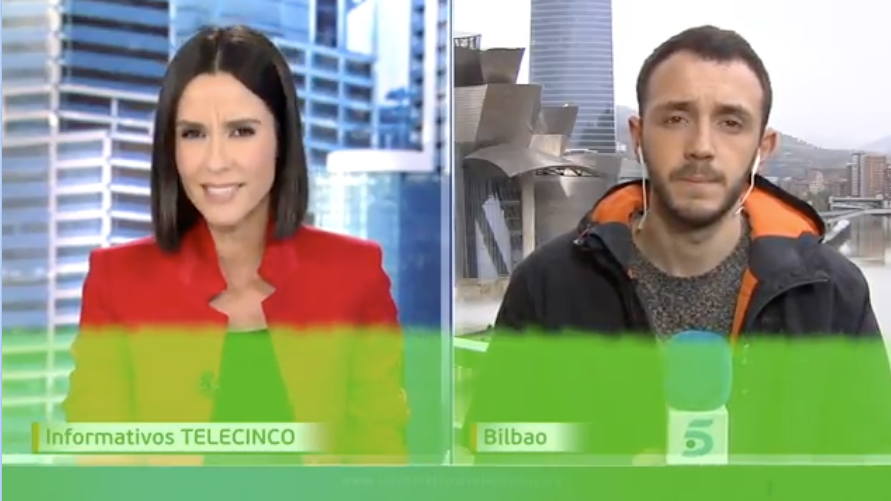
\includegraphics[width=100mm]{figures/image_recog}
		
		\caption*{\small Notes: Example of a image with a caption that delimits the beginning of a new section. The highlighted area shows the bottom of the image where image recognition can be applied to find such appearances.}
			\label{figure:image_rec}
	\end{figure} 
	
	
	
	
	\textbf{Speaker diarization}
	
	
	A less computationally expensive alternative consist on using \textit{speaker diarization} on the wav files. After transforming the mp4 file to audio using \textit{ffmpeg}, I use Google Cloud diarization tool to find the different speakers in an audio file. The most common (or most two common if it is a weekend) speakers overall corresponds to the presenter of the news. After allowing a flexible specification, one can identify break points by cheeking the seconds where the presenter comes back into scene making sure she is speaking long enough so that a new segment is being introduced. Figure \ref{fig:diarization} illustrates this procedure and the comparison with the manually annotated labels for an example day-channel.
	
	
	\begin{figure}[H]
		\centering
		\caption{Comparison audio splitting with annotated section splits}
		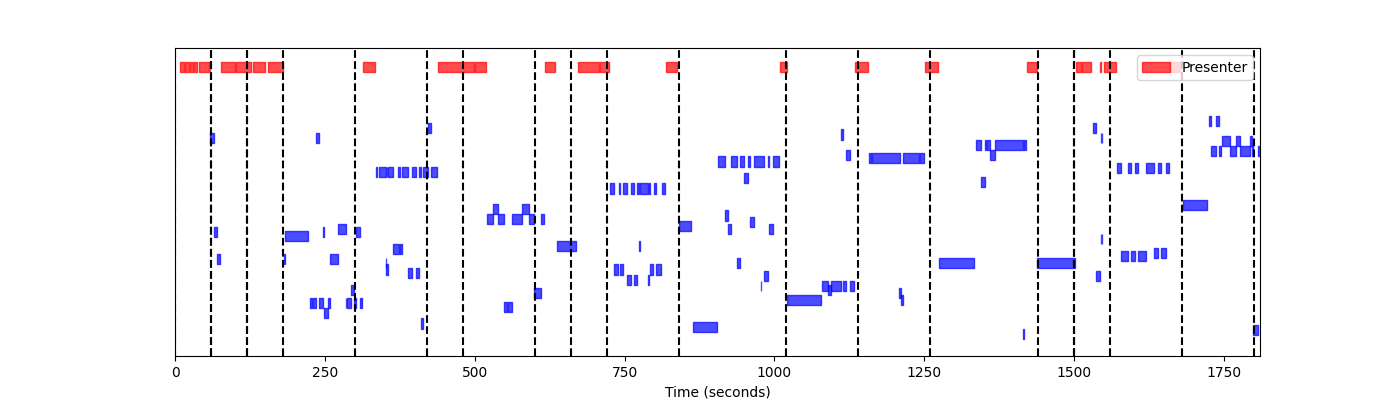
\includegraphics[width=120mm]{figures/speakers_all}
		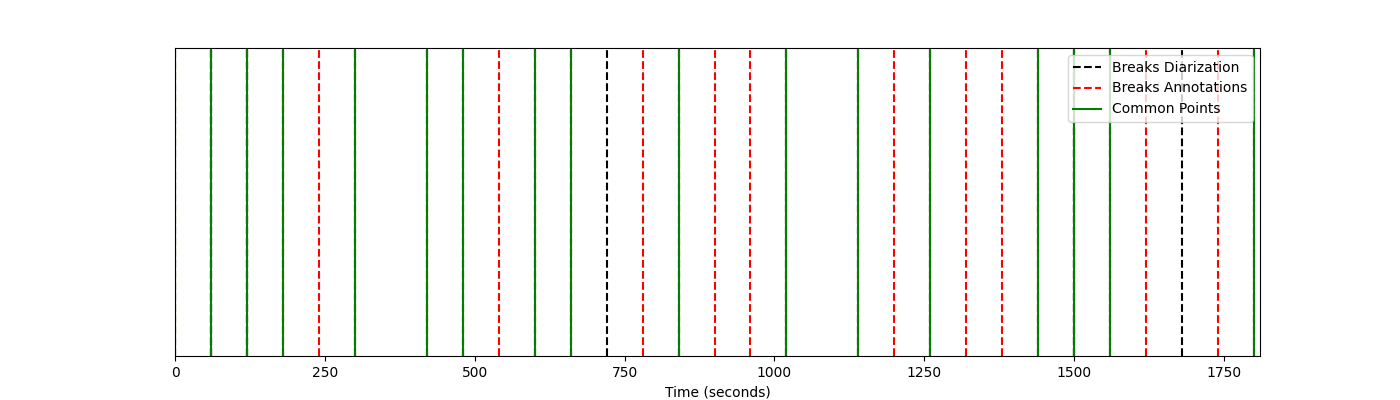
\includegraphics[width=120mm]{figures/speaker_timeline}
		\caption*{\small Notes: The top figure shows the timeline for the presenter audio (red) vs other audios recognized by \textit{speech2text} in a wav file for the 15th January 2023 in La Sexta. Vertical, black, dashed lines represent the predicted splits based on the diarization. The bottom figure combines these splits with the ones that come from the manually annotated figures. Red, dashed bars correspond to the breaks that come from the manually annotated GECA dataset. Green bars represent breaks where both the speaker diarization and the manual annotation coincide on a break. }
		\label{fig:diarization}
	\end{figure}
	
	
	
	
	\end{comment}
	
	
	
	
	
	
	
	
	
	
	

	
	
\end{document}